\documentclass[twoside]{book}

% Packages required by doxygen
\usepackage{calc}
\usepackage{doxygen}
\usepackage{graphicx}
\usepackage[utf8]{inputenc}
\usepackage{makeidx}
\usepackage{multicol}
\usepackage{multirow}
\usepackage{fixltx2e}
\PassOptionsToPackage{warn}{textcomp}
\usepackage{textcomp}
\usepackage[nointegrals]{wasysym}
\usepackage[table]{xcolor}

% Font selection
\usepackage[T1]{fontenc}
\usepackage{mathptmx}
\usepackage[scaled=.90]{helvet}
\usepackage{courier}
\usepackage{amssymb}
\usepackage{sectsty}
\renewcommand{\familydefault}{\sfdefault}
\allsectionsfont{%
  \fontseries{bc}\selectfont%
  \color{darkgray}%
}
\renewcommand{\DoxyLabelFont}{%
  \fontseries{bc}\selectfont%
  \color{darkgray}%
}
\newcommand{\+}{\discretionary{\mbox{\scriptsize$\hookleftarrow$}}{}{}}

% Page & text layout
\usepackage{geometry}
\geometry{%
  a4paper,%
  top=2.5cm,%
  bottom=2.5cm,%
  left=2.5cm,%
  right=2.5cm%
}
\tolerance=750
\hfuzz=15pt
\hbadness=750
\setlength{\emergencystretch}{15pt}
\setlength{\parindent}{0cm}
\setlength{\parskip}{0.2cm}
\makeatletter
\renewcommand{\paragraph}{%
  \@startsection{paragraph}{4}{0ex}{-1.0ex}{1.0ex}{%
    \normalfont\normalsize\bfseries\SS@parafont%
  }%
}
\renewcommand{\subparagraph}{%
  \@startsection{subparagraph}{5}{0ex}{-1.0ex}{1.0ex}{%
    \normalfont\normalsize\bfseries\SS@subparafont%
  }%
}
\makeatother

% Headers & footers
\usepackage{fancyhdr}
\pagestyle{fancyplain}
\fancyhead[LE]{\fancyplain{}{\bfseries\thepage}}
\fancyhead[CE]{\fancyplain{}{}}
\fancyhead[RE]{\fancyplain{}{\bfseries\leftmark}}
\fancyhead[LO]{\fancyplain{}{\bfseries\rightmark}}
\fancyhead[CO]{\fancyplain{}{}}
\fancyhead[RO]{\fancyplain{}{\bfseries\thepage}}
\fancyfoot[LE]{\fancyplain{}{}}
\fancyfoot[CE]{\fancyplain{}{}}
\fancyfoot[RE]{\fancyplain{}{\bfseries\scriptsize Generated on Wed Nov 2 2016 12\+:50\+:23 for Interface to D\+J\+A\+N\+G\+O\+H by Doxygen }}
\fancyfoot[LO]{\fancyplain{}{\bfseries\scriptsize Generated on Wed Nov 2 2016 12\+:50\+:23 for Interface to D\+J\+A\+N\+G\+O\+H by Doxygen }}
\fancyfoot[CO]{\fancyplain{}{}}
\fancyfoot[RO]{\fancyplain{}{}}
\renewcommand{\footrulewidth}{0.4pt}
\renewcommand{\chaptermark}[1]{%
  \markboth{#1}{}%
}
\renewcommand{\sectionmark}[1]{%
  \markright{\thesection\ #1}%
}

% Indices & bibliography
\usepackage{natbib}
\usepackage[titles]{tocloft}
\setcounter{tocdepth}{3}
\setcounter{secnumdepth}{5}
\makeindex

% Hyperlinks (required, but should be loaded last)
\usepackage{ifpdf}
\ifpdf
  \usepackage[pdftex,pagebackref=true]{hyperref}
\else
  \usepackage[ps2pdf,pagebackref=true]{hyperref}
\fi
\hypersetup{%
  colorlinks=true,%
  linkcolor=blue,%
  citecolor=blue,%
  unicode%
}

% Custom commands
\newcommand{\clearemptydoublepage}{%
  \newpage{\pagestyle{empty}\cleardoublepage}%
}


%===== C O N T E N T S =====

\begin{document}

% Titlepage & ToC
\hypersetup{pageanchor=false,
             bookmarks=true,
             bookmarksnumbered=true,
             pdfencoding=unicode
            }
\pagenumbering{roman}
\begin{titlepage}
\vspace*{7cm}
\begin{center}%
{\Large Interface to D\+J\+A\+N\+G\+O\+H \\[1ex]\large 0.\+1 }\\
\vspace*{1cm}
{\large Generated by Doxygen 1.8.7}\\
\vspace*{0.5cm}
{\small Wed Nov 2 2016 12:50:23}\\
\end{center}
\end{titlepage}
\clearemptydoublepage
\tableofcontents
\clearemptydoublepage
\pagenumbering{arabic}
\hypersetup{pageanchor=true}

%--- Begin generated contents ---
\chapter{Hierarchical Index}
\section{Class Hierarchy}
This inheritance list is sorted roughly, but not completely, alphabetically\+:\begin{DoxyCompactList}
\item \contentsline{section}{Djkin\+\_\+t}{\pageref{struct_djkin__t}}{}
\item \contentsline{section}{hsalfs}{\pageref{structhsalfs}}{}
\item \contentsline{section}{hselab}{\pageref{structhselab}}{}
\item \contentsline{section}{hselep}{\pageref{structhselep}}{}
\item \contentsline{section}{hsgrid}{\pageref{structhsgrid}}{}
\item \contentsline{section}{hsintcc}{\pageref{structhsintcc}}{}
\item \contentsline{section}{hsintnc}{\pageref{structhsintnc}}{}
\item \contentsline{section}{hsirct}{\pageref{structhsirct}}{}
\item \contentsline{section}{hsisgm}{\pageref{structhsisgm}}{}
\item \contentsline{section}{hslptu}{\pageref{structhslptu}}{}
\item \contentsline{section}{hsnucl}{\pageref{structhsnucl}}{}
\item \contentsline{section}{hsnume}{\pageref{structhsnume}}{}
\item \contentsline{section}{hsoptn}{\pageref{structhsoptn}}{}
\item \contentsline{section}{hsoutf}{\pageref{structhsoutf}}{}
\item \contentsline{section}{hsparl}{\pageref{structhsparl}}{}
\item \contentsline{section}{hsparm}{\pageref{structhsparm}}{}
\item \contentsline{section}{hspcut}{\pageref{structhspcut}}{}
\item \contentsline{section}{hspdfo}{\pageref{structhspdfo}}{}
\item \contentsline{section}{hsrdio}{\pageref{structhsrdio}}{}
\item \contentsline{section}{hssamcc}{\pageref{structhssamcc}}{}
\item \contentsline{section}{hssamnc}{\pageref{structhssamnc}}{}
\item \contentsline{section}{hsstrp}{\pageref{structhsstrp}}{}
\item \contentsline{section}{hstcut}{\pageref{structhstcut}}{}
\item \contentsline{section}{hsvglp}{\pageref{structhsvglp}}{}
\item \contentsline{section}{hsvrbz}{\pageref{structhsvrbz}}{}
\item \contentsline{section}{hswgtc}{\pageref{structhswgtc}}{}
\item \contentsline{section}{hystfu}{\pageref{structhystfu}}{}
\item \contentsline{section}{ihscut}{\pageref{structihscut}}{}
\item \contentsline{section}{ihscw}{\pageref{structihscw}}{}
\item \contentsline{section}{lhapdfc}{\pageref{structlhapdfc}}{}
\item \contentsline{section}{Ludat1\+\_\+t}{\pageref{struct_ludat1__t}}{}
\item \contentsline{section}{Ludat2\+\_\+t}{\pageref{struct_ludat2__t}}{}
\item \contentsline{section}{Lujets\+\_\+t}{\pageref{struct_lujets__t}}{}
\item \contentsline{section}{sophct}{\pageref{structsophct}}{}
\item \contentsline{section}{T\+Djangoh\+:\+:T\+Djangoh\+Cleaner}{\pageref{class_t_djangoh_1_1_t_djangoh_cleaner}}{}
\item T\+Generator\begin{DoxyCompactList}
\item \contentsline{section}{T\+Djangoh}{\pageref{class_t_djangoh}}{}
\end{DoxyCompactList}
\item \contentsline{section}{T\+M\+C\+Particle}{\pageref{class_t_m_c_particle}}{}
\item \contentsline{section}{xsectionmodule\+:\+:xsection2}{\pageref{structxsectionmodule_1_1xsection2}}{}
\item \contentsline{section}{xsectionmodule\+:\+:xsection2c}{\pageref{structxsectionmodule_1_1xsection2c}}{}
\item \contentsline{section}{xsectionmodule\+:\+:xsection2e}{\pageref{structxsectionmodule_1_1xsection2e}}{}
\item \contentsline{section}{xsectionmodule\+:\+:xsection31}{\pageref{structxsectionmodule_1_1xsection31}}{}
\item \contentsline{section}{xsectionmodule\+:\+:xsection31c}{\pageref{structxsectionmodule_1_1xsection31c}}{}
\item \contentsline{section}{xsectionmodule\+:\+:xsection31e}{\pageref{structxsectionmodule_1_1xsection31e}}{}
\item \contentsline{section}{xsectionmodule\+:\+:xsection32}{\pageref{structxsectionmodule_1_1xsection32}}{}
\item \contentsline{section}{xsectionmodule\+:\+:xsection32c}{\pageref{structxsectionmodule_1_1xsection32c}}{}
\item \contentsline{section}{xsectionmodule\+:\+:xsection32e}{\pageref{structxsectionmodule_1_1xsection32e}}{}
\item \contentsline{section}{xsectionmodule\+:\+:xsection33}{\pageref{structxsectionmodule_1_1xsection33}}{}
\item \contentsline{section}{xsectionmodule\+:\+:xsection33c}{\pageref{structxsectionmodule_1_1xsection33c}}{}
\item \contentsline{section}{xsectionmodule\+:\+:xsection33e}{\pageref{structxsectionmodule_1_1xsection33e}}{}
\item \contentsline{section}{xsectionmodule\+:\+:xsection34}{\pageref{structxsectionmodule_1_1xsection34}}{}
\end{DoxyCompactList}

\chapter{Class Index}
\section{Class List}
Here are the classes, structs, unions and interfaces with brief descriptions\+:\begin{DoxyCompactList}
\item\contentsline{section}{\hyperlink{struct_ludat1__t}{Ludat1\+\_\+t} \\*Djangoh common block Ludat1 }{\pageref{struct_ludat1__t}}{}
\item\contentsline{section}{\hyperlink{struct_ludat2__t}{Ludat2\+\_\+t} \\*Djangoh common block Ludat2 }{\pageref{struct_ludat2__t}}{}
\item\contentsline{section}{\hyperlink{struct_lujets__t}{Lujets\+\_\+t} \\*Djangoh common block Lujets }{\pageref{struct_lujets__t}}{}
\item\contentsline{section}{\hyperlink{class_t_djangoh}{T\+Djangoh} \\*C/\+C++ Interface to Djangoh }{\pageref{class_t_djangoh}}{}
\item\contentsline{section}{\hyperlink{class_t_djangoh_1_1_t_djangoh_cleaner}{T\+Djangoh\+::\+T\+Djangoh\+Cleaner} \\*A cleaner for \hyperlink{class_t_djangoh}{T\+Djangoh} }{\pageref{class_t_djangoh_1_1_t_djangoh_cleaner}}{}
\item\contentsline{section}{\hyperlink{class_t_m_c_particle}{T\+M\+C\+Particle} }{\pageref{class_t_m_c_particle}}{}
\end{DoxyCompactList}

\chapter{File Index}
\section{File List}
Here is a list of all files with brief descriptions\+:\begin{DoxyCompactList}
\item\contentsline{section}{include/\hyperlink{_t_djangoh_8h}{T\+Djangoh.\+h} \\*Interface class to Djangoh generator }{\pageref{_t_djangoh_8h}}{}
\item\contentsline{section}{include/\hyperlink{_t_djangoh_calls_8h}{T\+Djangoh\+Calls.\+h} \\*Storage of C++ structure mimicking F\+O\+R\+T\+R\+AN common blocks }{\pageref{_t_djangoh_calls_8h}}{}
\item\contentsline{section}{src/\hyperlink{djangoh__h_8f}{djangoh\+\_\+h.\+f} }{\pageref{djangoh__h_8f}}{}
\item\contentsline{section}{src/\hyperlink{djangoh__l_8f}{djangoh\+\_\+l.\+f} }{\pageref{djangoh__l_8f}}{}
\item\contentsline{section}{src/\hyperlink{djangoh__t_8f}{djangoh\+\_\+t.\+f} }{\pageref{djangoh__t_8f}}{}
\item\contentsline{section}{src/\hyperlink{djangoh__u_8f}{djangoh\+\_\+u.\+f} }{\pageref{djangoh__u_8f}}{}
\item\contentsline{section}{src/\hyperlink{_t_djangoh_8cc}{T\+Djangoh.\+cc} \\*Interface class to Djangoh generator }{\pageref{_t_djangoh_8cc}}{}
\item\contentsline{section}{src/\hyperlink{_t_m_c_particle_8cc}{T\+M\+C\+Particle.\+cc} }{\pageref{_t_m_c_particle_8cc}}{}
\item\contentsline{section}{src/\hyperlink{x_section_module_8f90}{x\+Section\+Module.\+f90} }{\pageref{x_section_module_8f90}}{}
\end{DoxyCompactList}

\chapter{Class Documentation}
\hypertarget{struct_ludat1__t}{\section{Ludat1\+\_\+t Struct Reference}
\label{struct_ludat1__t}\index{Ludat1\+\_\+t@{Ludat1\+\_\+t}}
}


Djangoh common block Ludat1.  




{\ttfamily \#include $<$T\+Djangoh\+Calls.\+h$>$}

\subsection*{Public Attributes}
\begin{DoxyCompactItemize}
\item 
int \hyperlink{struct_ludat1__t_ae01a3aee4bb22a760e8ea252207e2cd4}{M\+S\+T\+U} \mbox{[}200\mbox{]}
\item 
double \hyperlink{struct_ludat1__t_acde27cfd0ebacc6b76cdcb339044c627}{P\+A\+R\+U} \mbox{[}200\mbox{]}
\item 
int \hyperlink{struct_ludat1__t_ab47d0cbcea897c1d7f6993c63d8fb1d8}{M\+S\+T\+J} \mbox{[}200\mbox{]}
\item 
double \hyperlink{struct_ludat1__t_a3c1647b2c9d49467b84324857e22daaf}{P\+A\+R\+J} \mbox{[}200\mbox{]}
\end{DoxyCompactItemize}


\subsection{Detailed Description}
Djangoh common block Ludat1. 

\subsection{Member Data Documentation}
\hypertarget{struct_ludat1__t_ab47d0cbcea897c1d7f6993c63d8fb1d8}{\index{Ludat1\+\_\+t@{Ludat1\+\_\+t}!M\+S\+T\+J@{M\+S\+T\+J}}
\index{M\+S\+T\+J@{M\+S\+T\+J}!Ludat1\+\_\+t@{Ludat1\+\_\+t}}
\subsubsection[{M\+S\+T\+J}]{\setlength{\rightskip}{0pt plus 5cm}int Ludat1\+\_\+t\+::\+M\+S\+T\+J\mbox{[}200\mbox{]}}}\label{struct_ludat1__t_ab47d0cbcea897c1d7f6993c63d8fb1d8}
\hypertarget{struct_ludat1__t_ae01a3aee4bb22a760e8ea252207e2cd4}{\index{Ludat1\+\_\+t@{Ludat1\+\_\+t}!M\+S\+T\+U@{M\+S\+T\+U}}
\index{M\+S\+T\+U@{M\+S\+T\+U}!Ludat1\+\_\+t@{Ludat1\+\_\+t}}
\subsubsection[{M\+S\+T\+U}]{\setlength{\rightskip}{0pt plus 5cm}int Ludat1\+\_\+t\+::\+M\+S\+T\+U\mbox{[}200\mbox{]}}}\label{struct_ludat1__t_ae01a3aee4bb22a760e8ea252207e2cd4}
\hypertarget{struct_ludat1__t_a3c1647b2c9d49467b84324857e22daaf}{\index{Ludat1\+\_\+t@{Ludat1\+\_\+t}!P\+A\+R\+J@{P\+A\+R\+J}}
\index{P\+A\+R\+J@{P\+A\+R\+J}!Ludat1\+\_\+t@{Ludat1\+\_\+t}}
\subsubsection[{P\+A\+R\+J}]{\setlength{\rightskip}{0pt plus 5cm}double Ludat1\+\_\+t\+::\+P\+A\+R\+J\mbox{[}200\mbox{]}}}\label{struct_ludat1__t_a3c1647b2c9d49467b84324857e22daaf}
\hypertarget{struct_ludat1__t_acde27cfd0ebacc6b76cdcb339044c627}{\index{Ludat1\+\_\+t@{Ludat1\+\_\+t}!P\+A\+R\+U@{P\+A\+R\+U}}
\index{P\+A\+R\+U@{P\+A\+R\+U}!Ludat1\+\_\+t@{Ludat1\+\_\+t}}
\subsubsection[{P\+A\+R\+U}]{\setlength{\rightskip}{0pt plus 5cm}double Ludat1\+\_\+t\+::\+P\+A\+R\+U\mbox{[}200\mbox{]}}}\label{struct_ludat1__t_acde27cfd0ebacc6b76cdcb339044c627}


The documentation for this struct was generated from the following file\+:\begin{DoxyCompactItemize}
\item 
T\+Djangoh/\hyperlink{_t_djangoh_calls_8h}{T\+Djangoh\+Calls.\+h}\end{DoxyCompactItemize}

\hypertarget{struct_ludat2__t}{}\section{Ludat2\+\_\+t Struct Reference}
\label{struct_ludat2__t}\index{Ludat2\+\_\+t@{Ludat2\+\_\+t}}


Djangoh common block Ludat2.  




{\ttfamily \#include $<$T\+Djangoh\+Calls.\+h$>$}

\subsection*{Public Attributes}
\begin{DoxyCompactItemize}
\item 
int \hyperlink{struct_ludat2__t_ae7ac5c356f6954159345aa9043cde094}{K\+C\+HG} \mbox{[}4\mbox{]}\mbox{[}500\mbox{]}
\item 
double \hyperlink{struct_ludat2__t_a3ba40c50d21f9c3e2a9f27a1630e9199}{P\+M\+AS} \mbox{[}4\mbox{]}\mbox{[}500\mbox{]}
\item 
double \hyperlink{struct_ludat2__t_a1691485f7138c4707132de64991719e5}{P\+A\+RF} \mbox{[}2000\mbox{]}
\item 
double \hyperlink{struct_ludat2__t_a20d157be63ce36f91641642e81bb7334}{V\+C\+KM} \mbox{[}4\mbox{]}\mbox{[}4\mbox{]}
\end{DoxyCompactItemize}


\subsection{Detailed Description}
Djangoh common block Ludat2. 

\subsection{Member Data Documentation}
\mbox{\Hypertarget{struct_ludat2__t_ae7ac5c356f6954159345aa9043cde094}\label{struct_ludat2__t_ae7ac5c356f6954159345aa9043cde094}} 
\index{Ludat2\+\_\+t@{Ludat2\+\_\+t}!K\+C\+HG@{K\+C\+HG}}
\index{K\+C\+HG@{K\+C\+HG}!Ludat2\+\_\+t@{Ludat2\+\_\+t}}
\subsubsection{\texorpdfstring{K\+C\+HG}{KCHG}}
{\footnotesize\ttfamily int Ludat2\+\_\+t\+::\+K\+C\+HG\mbox{[}4\mbox{]}\mbox{[}500\mbox{]}}

\mbox{\Hypertarget{struct_ludat2__t_a1691485f7138c4707132de64991719e5}\label{struct_ludat2__t_a1691485f7138c4707132de64991719e5}} 
\index{Ludat2\+\_\+t@{Ludat2\+\_\+t}!P\+A\+RF@{P\+A\+RF}}
\index{P\+A\+RF@{P\+A\+RF}!Ludat2\+\_\+t@{Ludat2\+\_\+t}}
\subsubsection{\texorpdfstring{P\+A\+RF}{PARF}}
{\footnotesize\ttfamily double Ludat2\+\_\+t\+::\+P\+A\+RF\mbox{[}2000\mbox{]}}

\mbox{\Hypertarget{struct_ludat2__t_a3ba40c50d21f9c3e2a9f27a1630e9199}\label{struct_ludat2__t_a3ba40c50d21f9c3e2a9f27a1630e9199}} 
\index{Ludat2\+\_\+t@{Ludat2\+\_\+t}!P\+M\+AS@{P\+M\+AS}}
\index{P\+M\+AS@{P\+M\+AS}!Ludat2\+\_\+t@{Ludat2\+\_\+t}}
\subsubsection{\texorpdfstring{P\+M\+AS}{PMAS}}
{\footnotesize\ttfamily double Ludat2\+\_\+t\+::\+P\+M\+AS\mbox{[}4\mbox{]}\mbox{[}500\mbox{]}}

\mbox{\Hypertarget{struct_ludat2__t_a20d157be63ce36f91641642e81bb7334}\label{struct_ludat2__t_a20d157be63ce36f91641642e81bb7334}} 
\index{Ludat2\+\_\+t@{Ludat2\+\_\+t}!V\+C\+KM@{V\+C\+KM}}
\index{V\+C\+KM@{V\+C\+KM}!Ludat2\+\_\+t@{Ludat2\+\_\+t}}
\subsubsection{\texorpdfstring{V\+C\+KM}{VCKM}}
{\footnotesize\ttfamily double Ludat2\+\_\+t\+::\+V\+C\+KM\mbox{[}4\mbox{]}\mbox{[}4\mbox{]}}



The documentation for this struct was generated from the following file\+:\begin{DoxyCompactItemize}
\item 
include/\hyperlink{_t_djangoh_calls_8h}{T\+Djangoh\+Calls.\+h}\end{DoxyCompactItemize}

\hypertarget{struct_lujets__t}{\section{Lujets\+\_\+t Struct Reference}
\label{struct_lujets__t}\index{Lujets\+\_\+t@{Lujets\+\_\+t}}
}


Djangoh common block Lujets.  




{\ttfamily \#include $<$T\+Djangoh\+Calls.\+h$>$}

\subsection*{Public Attributes}
\begin{DoxyCompactItemize}
\item 
int \hyperlink{struct_lujets__t_a17571954fa27f93e7a5bdaf763057547}{N}
\item 
int \hyperlink{struct_lujets__t_a9bfadb28d8093e469dfed54f7df5b80e}{N\+P\+A\+D}
\item 
int \hyperlink{struct_lujets__t_ad8aaaaff1a45805c18b56154446bdf16}{K} \mbox{[}5\mbox{]}\mbox{[}4000\mbox{]}
\item 
double \hyperlink{struct_lujets__t_aec85d7058f39ff74657d6d7f8ef54d21}{P} \mbox{[}5\mbox{]}\mbox{[}4000\mbox{]}
\item 
double \hyperlink{struct_lujets__t_a0a2bde586f224cda7072d27ed5df78f5}{V} \mbox{[}5\mbox{]}\mbox{[}4000\mbox{]}
\end{DoxyCompactItemize}


\subsection{Detailed Description}
Djangoh common block Lujets. 

\subsection{Member Data Documentation}
\hypertarget{struct_lujets__t_ad8aaaaff1a45805c18b56154446bdf16}{\index{Lujets\+\_\+t@{Lujets\+\_\+t}!K@{K}}
\index{K@{K}!Lujets\+\_\+t@{Lujets\+\_\+t}}
\subsubsection[{K}]{\setlength{\rightskip}{0pt plus 5cm}int Lujets\+\_\+t\+::\+K\mbox{[}5\mbox{]}\mbox{[}4000\mbox{]}}}\label{struct_lujets__t_ad8aaaaff1a45805c18b56154446bdf16}
\hypertarget{struct_lujets__t_a17571954fa27f93e7a5bdaf763057547}{\index{Lujets\+\_\+t@{Lujets\+\_\+t}!N@{N}}
\index{N@{N}!Lujets\+\_\+t@{Lujets\+\_\+t}}
\subsubsection[{N}]{\setlength{\rightskip}{0pt plus 5cm}int Lujets\+\_\+t\+::\+N}}\label{struct_lujets__t_a17571954fa27f93e7a5bdaf763057547}
\hypertarget{struct_lujets__t_a9bfadb28d8093e469dfed54f7df5b80e}{\index{Lujets\+\_\+t@{Lujets\+\_\+t}!N\+P\+A\+D@{N\+P\+A\+D}}
\index{N\+P\+A\+D@{N\+P\+A\+D}!Lujets\+\_\+t@{Lujets\+\_\+t}}
\subsubsection[{N\+P\+A\+D}]{\setlength{\rightskip}{0pt plus 5cm}int Lujets\+\_\+t\+::\+N\+P\+A\+D}}\label{struct_lujets__t_a9bfadb28d8093e469dfed54f7df5b80e}
\hypertarget{struct_lujets__t_aec85d7058f39ff74657d6d7f8ef54d21}{\index{Lujets\+\_\+t@{Lujets\+\_\+t}!P@{P}}
\index{P@{P}!Lujets\+\_\+t@{Lujets\+\_\+t}}
\subsubsection[{P}]{\setlength{\rightskip}{0pt plus 5cm}double Lujets\+\_\+t\+::\+P\mbox{[}5\mbox{]}\mbox{[}4000\mbox{]}}}\label{struct_lujets__t_aec85d7058f39ff74657d6d7f8ef54d21}
\hypertarget{struct_lujets__t_a0a2bde586f224cda7072d27ed5df78f5}{\index{Lujets\+\_\+t@{Lujets\+\_\+t}!V@{V}}
\index{V@{V}!Lujets\+\_\+t@{Lujets\+\_\+t}}
\subsubsection[{V}]{\setlength{\rightskip}{0pt plus 5cm}double Lujets\+\_\+t\+::\+V\mbox{[}5\mbox{]}\mbox{[}4000\mbox{]}}}\label{struct_lujets__t_a0a2bde586f224cda7072d27ed5df78f5}


The documentation for this struct was generated from the following file\+:\begin{DoxyCompactItemize}
\item 
T\+Djangoh/\hyperlink{_t_djangoh_calls_8h}{T\+Djangoh\+Calls.\+h}\end{DoxyCompactItemize}

\hypertarget{class_t_djangoh}{}\section{T\+Djangoh Class Reference}
\label{class_t_djangoh}\index{T\+Djangoh@{T\+Djangoh}}


C/\+C++ Interface to Djangoh.  




{\ttfamily \#include $<$T\+Djangoh.\+h$>$}

Inheritance diagram for T\+Djangoh\+:\begin{figure}[H]
\begin{center}
\leavevmode
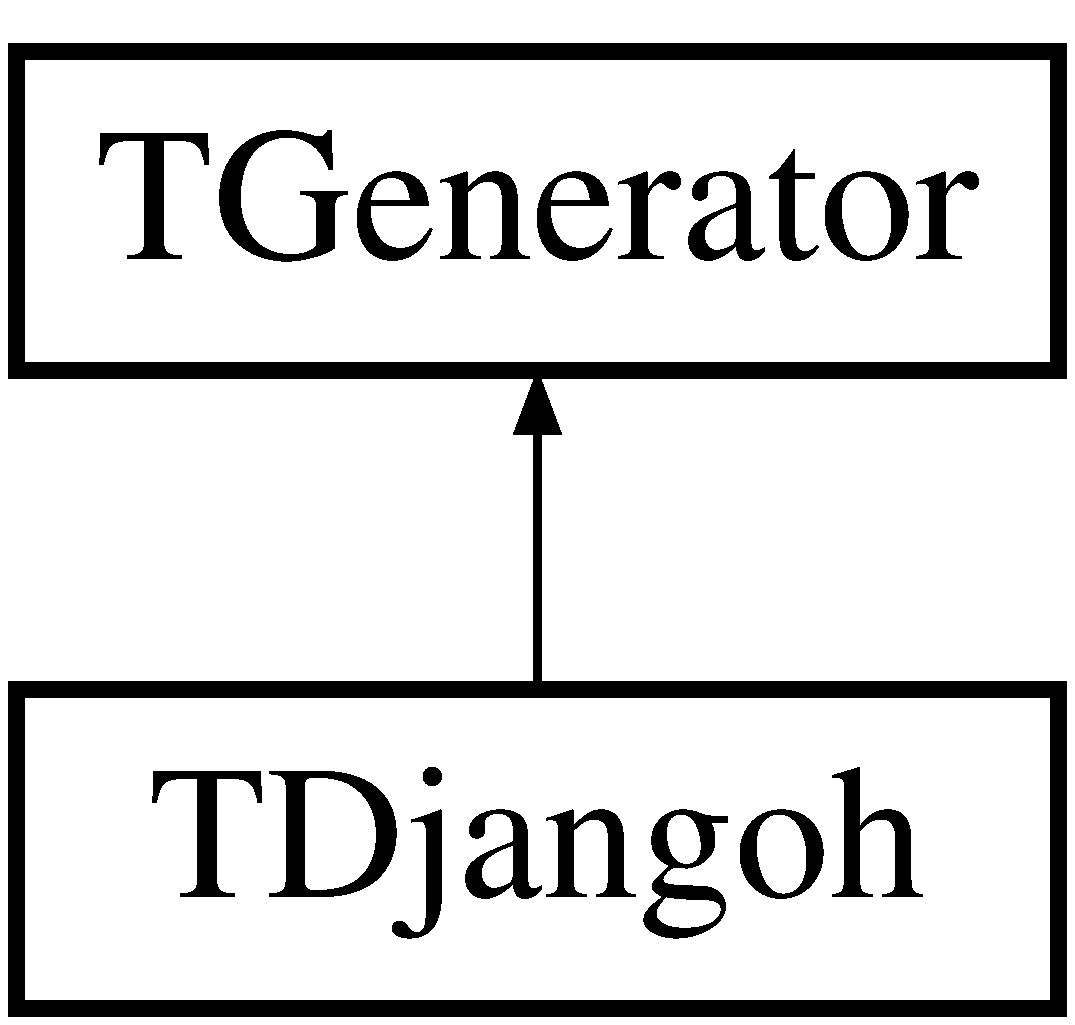
\includegraphics[height=2.000000cm]{class_t_djangoh}
\end{center}
\end{figure}
\subsection*{Classes}
\begin{DoxyCompactItemize}
\item 
class \hyperlink{class_t_djangoh_1_1_t_djangoh_cleaner}{T\+Djangoh\+Cleaner}
\begin{DoxyCompactList}\small\item\em A cleaner for \hyperlink{class_t_djangoh}{T\+Djangoh}. \end{DoxyCompactList}\end{DoxyCompactItemize}
\subsection*{Public Member Functions}
\begin{DoxyCompactItemize}
\item 
\hyperlink{class_t_djangoh_a7cbbb76ddc4fe82e25bb1e58078e45bc}{T\+Djangoh} ()
\begin{DoxyCompactList}\small\item\em Constructor of the \hyperlink{class_t_djangoh}{T\+Djangoh} class. \end{DoxyCompactList}\item 
virtual \hyperlink{class_t_djangoh_abee806f1e4536b30624590e34869f0e0}{$\sim$\+T\+Djangoh} ()
\begin{DoxyCompactList}\small\item\em Destructor of the \hyperlink{class_t_djangoh}{T\+Djangoh} class. \end{DoxyCompactList}\item 
void \hyperlink{class_t_djangoh_a121effe35c3f3ac168a4663bcd5eef5c}{Generate\+Event} ()
\begin{DoxyCompactList}\small\item\em Generation of an event. \end{DoxyCompactList}\item 
void \hyperlink{class_t_djangoh_a763cae78834404166df26ccd059bb301}{Initialize} ()
\begin{DoxyCompactList}\small\item\em Initialization of D\+J\+A\+N\+G\+OH. \end{DoxyCompactList}\item 
void \hyperlink{class_t_djangoh_af6954bed103bc5adc60822f16268c12d}{Read\+X\+M\+L\+File} (const string p\+Filename)
\begin{DoxyCompactList}\small\item\em Reading of parameters in X\+ML file. \end{DoxyCompactList}\item 
void \hyperlink{class_t_djangoh_ade135fa317b5678c048d417fcef573ae}{Write\+X\+M\+L\+File} (const string p\+Filename)
\item 
void \hyperlink{class_t_djangoh_a20fbc4c9736f639e6211333c6113421a}{Mod\+Kine\+Cuts} (int pcut, double pxmin, double pxmax, double pymin, double pymax, double pq2min, double pq2max, double pwmin)
\begin{DoxyCompactList}\small\item\em Modification of kinematical cuts. \end{DoxyCompactList}\item 
void \hyperlink{class_t_djangoh_acbf402e049af75c65f28589178eb1487}{Born\+W\+Oqel\+NC} ()
\begin{DoxyCompactList}\small\item\em Configuration for Born w/o quasielastic contribution generation. \end{DoxyCompactList}\item 
void \hyperlink{class_t_djangoh_a283b09ffc625a6a14af2f301ae957c92}{R\+Clep\+W\+Oqel\+NC} ()
\begin{DoxyCompactList}\small\item\em Configuration for leptonic RC w/o quasielastic contribution generation. \end{DoxyCompactList}\item 
void \hyperlink{class_t_djangoh_af58a4c6bb944a4ce79cc538829e490e8}{Configure} (float beam\+\_\+e, float pol)
\begin{DoxyCompactList}\small\item\em Configuration of D\+J\+A\+N\+G\+OH. \end{DoxyCompactList}\item 
void \hyperlink{class_t_djangoh_a076cac82063ed8740ac0a32e77c02c94}{End\+Recap} ()
\begin{DoxyCompactList}\small\item\em Print a recap of the generation made. \end{DoxyCompactList}\item 
Int\+\_\+t \hyperlink{class_t_djangoh_a69e5ebe63faa2dd00d9bcd217ecdf825}{Import\+Particles} (T\+Clones\+Array $\ast$particles, Option\+\_\+t $\ast$option=\char`\"{}\char`\"{})
\begin{DoxyCompactList}\small\item\em Import particles from lujets\+\_\+ subroutine and copy it in T\+Clones\+Array$\ast$. \end{DoxyCompactList}\item 
T\+Obj\+Array $\ast$ \hyperlink{class_t_djangoh_ac63f2c463b6a2fff98f256952aaf945f}{Import\+Particles} (Option\+\_\+t $\ast$option=\char`\"{}\char`\"{})
\begin{DoxyCompactList}\small\item\em Import particles from lujets\+\_\+ subroutine and copy it in T\+Clones\+Array$\ast$. \end{DoxyCompactList}\item 
double \hyperlink{class_t_djangoh_a6c3ac520ed9c8c8eb0e80f3dda7eb146}{Get\+Sigtot} ()
\begin{DoxyCompactList}\small\item\em Access total Cross-\/\+Section. \end{DoxyCompactList}\item 
double \hyperlink{class_t_djangoh_af888193a486499c7b019b0da80eae760}{Get\+Sigtrr} ()
\begin{DoxyCompactList}\small\item\em Access error on Cross-\/\+Section. \end{DoxyCompactList}\item 
int \hyperlink{class_t_djangoh_a2ed9a38fa1593d5a6a6e2c33b2912d1b}{Get\+Beam\+Type} ()
\begin{DoxyCompactList}\small\item\em Access beam particle type. \end{DoxyCompactList}\item 
void \hyperlink{class_t_djangoh_af93ae6412c07af22bca887cbcbba5082}{Set\+Beam\+Type} (int pvalue)
\begin{DoxyCompactList}\small\item\em Set beam particle type. \end{DoxyCompactList}\item 
void \hyperlink{class_t_djangoh_a37c2f8994175d3181a7f6f5aae5797f1}{Set\+Beam\+Type} (const char $\ast$pvalue)
\begin{DoxyCompactList}\small\item\em Set beam particle type. \end{DoxyCompactList}\item 
void \hyperlink{class_t_djangoh_a6995df5cd413a9e998fe8c0836004363}{Set\+Beam} (double p\+BeamE, double p\+Pol)
\begin{DoxyCompactList}\small\item\em Set beam energy and polarization. \end{DoxyCompactList}\item 
double \hyperlink{class_t_djangoh_a62b52fce9e36c0c7296fc1e519b1b902}{Get\+Beam\+Polar} ()
\begin{DoxyCompactList}\small\item\em Access beam polarization. \end{DoxyCompactList}\item 
double \hyperlink{class_t_djangoh_a34a0415a20f61670164665904eeca25b}{Set\+Beam\+Polar} (double pvalue)
\begin{DoxyCompactList}\small\item\em Set beam polarization. \end{DoxyCompactList}\item 
double \hyperlink{class_t_djangoh_a6baf26c760e0fc2f7bfc802fe7b14093}{Get\+Kinem\+Cut} (int i)
\begin{DoxyCompactList}\small\item\em Access kinematical cuts. \end{DoxyCompactList}\item 
void \hyperlink{class_t_djangoh_acb1c8c1ead16a0fbadd733b117cc0445}{Set\+Kinem\+Cut} (double pvalue, int i)
\begin{DoxyCompactList}\small\item\em Set kinematical cuts. \end{DoxyCompactList}\item 
double \hyperlink{class_t_djangoh_a74a77949c408cc303ec5e90482b1e639}{Get\+Gd\+Opt} (int i)
\begin{DoxyCompactList}\small\item\em Access cross-\/section grid values. \end{DoxyCompactList}\item 
void \hyperlink{class_t_djangoh_abbbe8452bf4a894e8757e096fb104d90}{Set\+Gd\+Opt} (double pvalue, int i)
\begin{DoxyCompactList}\small\item\em Set cross-\/section grid values. \end{DoxyCompactList}\item 
int \hyperlink{class_t_djangoh_ac58587b988731552d41321364c30748d}{Get\+Gsw} (int i)
\begin{DoxyCompactList}\small\item\em Access EW parameters values. \end{DoxyCompactList}\item 
void \hyperlink{class_t_djangoh_acbd9827496878eed7768c97031a1c1d7}{Set\+Gsw} (int pvalue, int i)
\begin{DoxyCompactList}\small\item\em Set EW parameters values. \end{DoxyCompactList}\item 
double \hyperlink{class_t_djangoh_a47b4a219c93cbcad58a82bfab9649a42}{Get\+Egam\+Min} ()
\begin{DoxyCompactList}\small\item\em Access cutoff energy value. \end{DoxyCompactList}\item 
void \hyperlink{class_t_djangoh_ac296a00fee7971d387aa5127f726a649}{Set\+Egam\+Min} (double pvalue)
\begin{DoxyCompactList}\small\item\em Set cutoff energy value. \end{DoxyCompactList}\item 
int \hyperlink{class_t_djangoh_aea74b082287a6870a27b07217832768f}{Get\+Int\+Opt\+NC} (int i)
\begin{DoxyCompactList}\small\item\em Access contribution to NC interactions values. \end{DoxyCompactList}\item 
void \hyperlink{class_t_djangoh_a867c7f0d6deb79773b4529e496a2ee23}{Set\+Int\+Opt\+NC} (int pvalue, int i)
\begin{DoxyCompactList}\small\item\em Set contribution to NC interactions values. \end{DoxyCompactList}\item 
void \hyperlink{class_t_djangoh_a6e6fa7e1826bd4e86be44d80a6bd6854}{Set\+Sam\+Opt\+NC} (int pvalue, int i)
\begin{DoxyCompactList}\small\item\em Set inclusion of NC cross-\/section to sampling values. \end{DoxyCompactList}\item 
int \hyperlink{class_t_djangoh_a58e1925539d208ca8e00533b5ae52074}{Get\+Struct\+Func} (int i)
\begin{DoxyCompactList}\small\item\em Access parametrization of structure functions values. \end{DoxyCompactList}\item 
void \hyperlink{class_t_djangoh_aa8331885aeb7880a63ebdfcf32919f9b}{Set\+Struct\+Func} (int pvalue, int i)
\begin{DoxyCompactList}\small\item\em Set parametrization of structure functions values. \end{DoxyCompactList}\item 
double \hyperlink{class_t_djangoh_a31acc70811ad58a8986f7d04547e9213}{Get\+Sophia} ()
\begin{DoxyCompactList}\small\item\em Access low W limit for Sophia value. \end{DoxyCompactList}\item 
void \hyperlink{class_t_djangoh_a12bd5515ab5db50b147810e06e98a0b8}{Set\+Sophia} (double pvalue)
\begin{DoxyCompactList}\small\item\em Set low W limit for Sophia value. \end{DoxyCompactList}\item 
int \hyperlink{class_t_djangoh_a1caf80b8f7228dbc7818ac047de9b8b7}{Get\+Verbose} ()
\begin{DoxyCompactList}\small\item\em Get verbose value. \end{DoxyCompactList}\item 
void \hyperlink{class_t_djangoh_a5129257c110777c1625049fb74f33e4b}{Set\+Verbose} (int pvalue)
\begin{DoxyCompactList}\small\item\em Set verbose value. \end{DoxyCompactList}\item 
int \hyperlink{class_t_djangoh_a39b356c5689222e6c82172e9b4954fe1}{Get\+Int\+Opt\+CC} (int i)
\begin{DoxyCompactList}\small\item\em Access contribution to CC interactions values. \end{DoxyCompactList}\item 
void \hyperlink{class_t_djangoh_a7e37a7afc5c112a2bd061f5e73973f78}{Set\+Int\+Opt\+CC} (int pvalue, int i)
\begin{DoxyCompactList}\small\item\em Set contribution to CC interactions values. \end{DoxyCompactList}\item 
void \hyperlink{class_t_djangoh_acc7a3124293fe30c297fb7702bade781}{Set\+Sam\+Opt\+CC} (int pvalue, int i)
\begin{DoxyCompactList}\small\item\em Set inclusion of CC cross-\/section to sampling values. \end{DoxyCompactList}\item 
void \hyperlink{class_t_djangoh_ae37cb56d62427ac672155e0817f6849e}{Set\+Nucleus} (double p\+Hpolar, int p\+Hna, int p\+Hnz, double p\+Epro=0)
\begin{DoxyCompactList}\small\item\em Set nucleus properties values. \end{DoxyCompactList}\item 
void \hyperlink{class_t_djangoh_aa78f3a43ed71499a9efe9e87cc22d668}{Write\+F\+S\+In\+File} ()
\begin{DoxyCompactList}\small\item\em Save final state infos in file. \end{DoxyCompactList}\item 
void \hyperlink{class_t_djangoh_ade1e9ff8b29d2b95d24a22c3474a7ba6}{Clean\+F\+S\+File} ()
\begin{DoxyCompactList}\small\item\em Remove final state file. \end{DoxyCompactList}\item 
double \hyperlink{class_t_djangoh_acf17f3e8d6a10ebe25f57f75662a1817}{Get\+P\+H\+EP} (int ip, int i)
\begin{DoxyCompactList}\small\item\em Access P\+H\+EP content of event. \end{DoxyCompactList}\item 
double \hyperlink{class_t_djangoh_ab8bbab97c50a6a9f296fbd0d78e98e17}{Get\+V\+H\+KK} (int ip, int i)
\begin{DoxyCompactList}\small\item\em Access V\+H\+KK content of event. \end{DoxyCompactList}\item 
int \hyperlink{class_t_djangoh_aaa275337568bcd47d87a63f1de688d27}{Get\+I\+D\+P\+H\+EP} (int i)
\begin{DoxyCompactList}\small\item\em Access I\+D\+P\+H\+EP content of event. \end{DoxyCompactList}\item 
int \hyperlink{class_t_djangoh_a381b6da1d6ef7145d9b4e49afb44a654}{Get\+Channel} ()
\begin{DoxyCompactList}\small\item\em Access sampling channel from Djangoh. \end{DoxyCompactList}\item 
void \hyperlink{class_t_djangoh_adf5acc5294013735f2475d4ce8ccf012}{Clean\+\_\+\+File} ()
\begin{DoxyCompactList}\small\item\em Clean files created by djangoh. \end{DoxyCompactList}\item 
\hyperlink{struct_lujets__t}{Lujets\+\_\+t} $\ast$ \hyperlink{class_t_djangoh_a2572e682379a304f84f21840d488fa0c}{Get\+Lujets} ()
\begin{DoxyCompactList}\small\item\em Recover the actual \hyperlink{struct_lujets__t}{Lujets\+\_\+t} structure. \end{DoxyCompactList}\item 
int \hyperlink{class_t_djangoh_a501e50bbb1ad6a75014fd7c555313b74}{GetN} ()
\begin{DoxyCompactList}\small\item\em Recover the number of particles. \end{DoxyCompactList}\item 
int \hyperlink{class_t_djangoh_afb58be11a10e8a6a4b442ea0fe4e16f5}{Get\+N\+P\+AD} ()
\begin{DoxyCompactList}\small\item\em Recover. \end{DoxyCompactList}\item 
int \hyperlink{class_t_djangoh_aaf2c94dbb8382bbd3b7ed1530a8ac878}{GetK} (int ip, int i)
\begin{DoxyCompactList}\small\item\em Access K content of event. \end{DoxyCompactList}\item 
double \hyperlink{class_t_djangoh_a2bc14d05d493e604f9f7fef847c19c9b}{GetP} (int ip, int i)
\begin{DoxyCompactList}\small\item\em Access P content of event. \end{DoxyCompactList}\item 
double \hyperlink{class_t_djangoh_a4993a87fef8917b9ed8a55811aa2daf6}{GetV} (int ip, int i)
\begin{DoxyCompactList}\small\item\em Access V content of event. \end{DoxyCompactList}\item 
void \hyperlink{class_t_djangoh_ac15b9862e954349fd9f0911c71e0e664}{SetN} (int n)
\begin{DoxyCompactList}\small\item\em Set the number of particles. \end{DoxyCompactList}\item 
void \hyperlink{class_t_djangoh_a0ed7bb7e7433a6385b5838ce519168a2}{Set\+N\+P\+AD} (int n)
\begin{DoxyCompactList}\small\item\em Set N\+P\+AD. \end{DoxyCompactList}\item 
void \hyperlink{class_t_djangoh_a045a7fabe350589453e240bff98ca54b}{SetK} (int ip, int i, int k)
\begin{DoxyCompactList}\small\item\em Set K content of event. \end{DoxyCompactList}\item 
void \hyperlink{class_t_djangoh_aa9cfa62ac6bf01a7f5214cc62cdae34c}{SetP} (int ip, int i, double p)
\begin{DoxyCompactList}\small\item\em Set P content of event. \end{DoxyCompactList}\item 
void \hyperlink{class_t_djangoh_a472e228f316f1473c940dfa37c22637c}{SetV} (int ip, int i, double v)
\begin{DoxyCompactList}\small\item\em Set V content of event. \end{DoxyCompactList}\item 
\hyperlink{struct_djkin__t}{Djkin\+\_\+t} $\ast$ \hyperlink{class_t_djangoh_a4f5a22f9af97e7c84660c94cd354f780}{Get\+Djkin} ()
\item 
double \hyperlink{class_t_djangoh_aa2d4a28a97826cf32b9d623c581da9de}{GetX} ()
\item 
double \hyperlink{class_t_djangoh_aee089d5536e8acb68236f9546e4f06e2}{GetY} ()
\item 
double \hyperlink{class_t_djangoh_a94c252e7c5375e9641ad5ea048098c06}{Get\+W2} ()
\item 
double \hyperlink{class_t_djangoh_afce6f0bfed90b20eb0f9310ae107291d}{Get\+Q2} ()
\item 
double \hyperlink{class_t_djangoh_a6e69090ac8581a1be96cac889cf5292b}{GetU} ()
\item 
double \hyperlink{class_t_djangoh_a64b580157191cf32f0b3ba4047b69bdf}{Get\+X\+H\+AD} ()
\item 
double \hyperlink{class_t_djangoh_a4cfb37ad76ec038f6e05b90341befb7f}{Get\+Y\+H\+AD} ()
\item 
double \hyperlink{class_t_djangoh_a969e748da53637a3732a27cfe23a34d2}{Get\+Q2\+H\+AD} ()
\item 
void \hyperlink{class_t_djangoh_a1ef3828a15dfd67a5e5c902bd584fd8b}{SetX} (double x)
\item 
void \hyperlink{class_t_djangoh_a91061fe2a386a9ddb7c7398c9443fa74}{SetY} (double y)
\item 
void \hyperlink{class_t_djangoh_aea9a499dfc8cbca480f228b79a05d99a}{Set\+W2} (double w)
\item 
void \hyperlink{class_t_djangoh_abecf2835ceecd72f0847544b72fd837e}{Set\+Q2} (double q)
\item 
void \hyperlink{class_t_djangoh_a69cebdc5dc26bfd0def872a996da0650}{SetU} (double u)
\item 
void \hyperlink{class_t_djangoh_a13173ef3490a98d8488ce7421905284c}{Set\+X\+H\+AD} (double x)
\item 
void \hyperlink{class_t_djangoh_a2dc4b62cd66dd41e8ae3d62965e36617}{Set\+Y\+H\+AD} (double y)
\item 
void \hyperlink{class_t_djangoh_a0066b103b2f779d8ed302fd77f42ee5e}{Set\+Q2\+H\+AD} (double q)
\end{DoxyCompactItemize}
\subsection*{Static Public Member Functions}
\begin{DoxyCompactItemize}
\item 
static \hyperlink{class_t_djangoh}{T\+Djangoh} $\ast$ \hyperlink{class_t_djangoh_a2e9871b8bec6326bb518f218dc87402c}{Instance} ()
\begin{DoxyCompactList}\small\item\em Instance creation. \end{DoxyCompactList}\end{DoxyCompactItemize}
\subsection*{Protected Member Functions}
\begin{DoxyCompactItemize}
\item 
\hyperlink{class_t_djangoh_a7b47ea508e2047b99b6f3efd6ba37278}{T\+Djangoh} (const \hyperlink{class_t_djangoh}{T\+Djangoh} \&)
\begin{DoxyCompactList}\small\item\em Copy Constructor of the \hyperlink{class_t_djangoh}{T\+Djangoh} class. \end{DoxyCompactList}\item 
\hyperlink{class_t_djangoh}{T\+Djangoh} \& \hyperlink{class_t_djangoh_a987204dc283979db28c83e5a35177b7c}{operator=} (const \hyperlink{class_t_djangoh}{T\+Djangoh} \&)
\begin{DoxyCompactList}\small\item\em = operator overload \end{DoxyCompactList}\end{DoxyCompactItemize}
\subsection*{Protected Attributes}
\begin{DoxyCompactItemize}
\item 
\hyperlink{struct_lujets__t}{Lujets\+\_\+t} $\ast$ \hyperlink{class_t_djangoh_a844cd27abcd743028fb98b3fba0c0fa9}{f\+Lujets}
\item 
\hyperlink{struct_djkin__t}{Djkin\+\_\+t} $\ast$ \hyperlink{class_t_djangoh_a870f9e5b91afdae5f21c10daae7c5d7e}{f\+Djkin}
\end{DoxyCompactItemize}
\subsection*{Static Protected Attributes}
\begin{DoxyCompactItemize}
\item 
static \hyperlink{class_t_djangoh}{T\+Djangoh} $\ast$ \hyperlink{class_t_djangoh_ad154e9fce28f84ab490dc6508db58fb8}{fg\+Instance} = 0
\end{DoxyCompactItemize}


\subsection{Detailed Description}
C/\+C++ Interface to Djangoh. 

\subsection{Constructor \& Destructor Documentation}
\mbox{\Hypertarget{class_t_djangoh_a7b47ea508e2047b99b6f3efd6ba37278}\label{class_t_djangoh_a7b47ea508e2047b99b6f3efd6ba37278}} 
\index{T\+Djangoh@{T\+Djangoh}!T\+Djangoh@{T\+Djangoh}}
\index{T\+Djangoh@{T\+Djangoh}!T\+Djangoh@{T\+Djangoh}}
\subsubsection{\texorpdfstring{T\+Djangoh()}{TDjangoh()}\hspace{0.1cm}{\footnotesize\ttfamily [1/2]}}
{\footnotesize\ttfamily T\+Djangoh\+::\+T\+Djangoh (\begin{DoxyParamCaption}\item[{const \hyperlink{class_t_djangoh}{T\+Djangoh} \&}]{dj }\end{DoxyParamCaption})\hspace{0.3cm}{\ttfamily [protected]}}



Copy Constructor of the \hyperlink{class_t_djangoh}{T\+Djangoh} class. 


\begin{DoxyParams}{Parameters}
{\em \hyperlink{class_t_djangoh}{T\+Djangoh}} & \+: \hyperlink{class_t_djangoh}{T\+Djangoh} object \\
\hline
\end{DoxyParams}
\mbox{\Hypertarget{class_t_djangoh_a7cbbb76ddc4fe82e25bb1e58078e45bc}\label{class_t_djangoh_a7cbbb76ddc4fe82e25bb1e58078e45bc}} 
\index{T\+Djangoh@{T\+Djangoh}!T\+Djangoh@{T\+Djangoh}}
\index{T\+Djangoh@{T\+Djangoh}!T\+Djangoh@{T\+Djangoh}}
\subsubsection{\texorpdfstring{T\+Djangoh()}{TDjangoh()}\hspace{0.1cm}{\footnotesize\ttfamily [2/2]}}
{\footnotesize\ttfamily T\+Djangoh\+::\+T\+Djangoh (\begin{DoxyParamCaption}{ }\end{DoxyParamCaption})}



Constructor of the \hyperlink{class_t_djangoh}{T\+Djangoh} class. 

\mbox{\Hypertarget{class_t_djangoh_abee806f1e4536b30624590e34869f0e0}\label{class_t_djangoh_abee806f1e4536b30624590e34869f0e0}} 
\index{T\+Djangoh@{T\+Djangoh}!````~T\+Djangoh@{$\sim$\+T\+Djangoh}}
\index{````~T\+Djangoh@{$\sim$\+T\+Djangoh}!T\+Djangoh@{T\+Djangoh}}
\subsubsection{\texorpdfstring{$\sim$\+T\+Djangoh()}{~TDjangoh()}}
{\footnotesize\ttfamily T\+Djangoh\+::$\sim$\+T\+Djangoh (\begin{DoxyParamCaption}{ }\end{DoxyParamCaption})\hspace{0.3cm}{\ttfamily [virtual]}}



Destructor of the \hyperlink{class_t_djangoh}{T\+Djangoh} class. 



\subsection{Member Function Documentation}
\mbox{\Hypertarget{class_t_djangoh_acbf402e049af75c65f28589178eb1487}\label{class_t_djangoh_acbf402e049af75c65f28589178eb1487}} 
\index{T\+Djangoh@{T\+Djangoh}!Born\+W\+Oqel\+NC@{Born\+W\+Oqel\+NC}}
\index{Born\+W\+Oqel\+NC@{Born\+W\+Oqel\+NC}!T\+Djangoh@{T\+Djangoh}}
\subsubsection{\texorpdfstring{Born\+W\+Oqel\+N\+C()}{BornWOqelNC()}}
{\footnotesize\ttfamily void T\+Djangoh\+::\+Born\+W\+Oqel\+NC (\begin{DoxyParamCaption}{ }\end{DoxyParamCaption})}



Configuration for Born w/o quasielastic contribution generation. 

\mbox{\Hypertarget{class_t_djangoh_adf5acc5294013735f2475d4ce8ccf012}\label{class_t_djangoh_adf5acc5294013735f2475d4ce8ccf012}} 
\index{T\+Djangoh@{T\+Djangoh}!Clean\+\_\+\+File@{Clean\+\_\+\+File}}
\index{Clean\+\_\+\+File@{Clean\+\_\+\+File}!T\+Djangoh@{T\+Djangoh}}
\subsubsection{\texorpdfstring{Clean\+\_\+\+File()}{Clean\_File()}}
{\footnotesize\ttfamily void T\+Djangoh\+::\+Clean\+\_\+\+File (\begin{DoxyParamCaption}{ }\end{DoxyParamCaption})}



Clean files created by djangoh. 

\mbox{\Hypertarget{class_t_djangoh_ade1e9ff8b29d2b95d24a22c3474a7ba6}\label{class_t_djangoh_ade1e9ff8b29d2b95d24a22c3474a7ba6}} 
\index{T\+Djangoh@{T\+Djangoh}!Clean\+F\+S\+File@{Clean\+F\+S\+File}}
\index{Clean\+F\+S\+File@{Clean\+F\+S\+File}!T\+Djangoh@{T\+Djangoh}}
\subsubsection{\texorpdfstring{Clean\+F\+S\+File()}{CleanFSFile()}}
{\footnotesize\ttfamily void T\+Djangoh\+::\+Clean\+F\+S\+File (\begin{DoxyParamCaption}{ }\end{DoxyParamCaption})\hspace{0.3cm}{\ttfamily [inline]}}



Remove final state file. 

\mbox{\Hypertarget{class_t_djangoh_af58a4c6bb944a4ce79cc538829e490e8}\label{class_t_djangoh_af58a4c6bb944a4ce79cc538829e490e8}} 
\index{T\+Djangoh@{T\+Djangoh}!Configure@{Configure}}
\index{Configure@{Configure}!T\+Djangoh@{T\+Djangoh}}
\subsubsection{\texorpdfstring{Configure()}{Configure()}}
{\footnotesize\ttfamily void T\+Djangoh\+::\+Configure (\begin{DoxyParamCaption}\item[{float}]{beam\+\_\+e,  }\item[{float}]{pol }\end{DoxyParamCaption})}



Configuration of D\+J\+A\+N\+G\+OH. 


\begin{DoxyParams}{Parameters}
{\em beam\+\_\+e} & \+: Energy of the beam (in GeV) \\
\hline
\end{DoxyParams}
\mbox{\Hypertarget{class_t_djangoh_a076cac82063ed8740ac0a32e77c02c94}\label{class_t_djangoh_a076cac82063ed8740ac0a32e77c02c94}} 
\index{T\+Djangoh@{T\+Djangoh}!End\+Recap@{End\+Recap}}
\index{End\+Recap@{End\+Recap}!T\+Djangoh@{T\+Djangoh}}
\subsubsection{\texorpdfstring{End\+Recap()}{EndRecap()}}
{\footnotesize\ttfamily void T\+Djangoh\+::\+End\+Recap (\begin{DoxyParamCaption}{ }\end{DoxyParamCaption})}



Print a recap of the generation made. 

\mbox{\Hypertarget{class_t_djangoh_a121effe35c3f3ac168a4663bcd5eef5c}\label{class_t_djangoh_a121effe35c3f3ac168a4663bcd5eef5c}} 
\index{T\+Djangoh@{T\+Djangoh}!Generate\+Event@{Generate\+Event}}
\index{Generate\+Event@{Generate\+Event}!T\+Djangoh@{T\+Djangoh}}
\subsubsection{\texorpdfstring{Generate\+Event()}{GenerateEvent()}}
{\footnotesize\ttfamily void T\+Djangoh\+::\+Generate\+Event (\begin{DoxyParamCaption}{ }\end{DoxyParamCaption})}



Generation of an event. 

\mbox{\Hypertarget{class_t_djangoh_a62b52fce9e36c0c7296fc1e519b1b902}\label{class_t_djangoh_a62b52fce9e36c0c7296fc1e519b1b902}} 
\index{T\+Djangoh@{T\+Djangoh}!Get\+Beam\+Polar@{Get\+Beam\+Polar}}
\index{Get\+Beam\+Polar@{Get\+Beam\+Polar}!T\+Djangoh@{T\+Djangoh}}
\subsubsection{\texorpdfstring{Get\+Beam\+Polar()}{GetBeamPolar()}}
{\footnotesize\ttfamily double T\+Djangoh\+::\+Get\+Beam\+Polar (\begin{DoxyParamCaption}{ }\end{DoxyParamCaption})}



Access beam polarization. 

\begin{DoxyReturn}{Returns}
Beam polarization 
\end{DoxyReturn}
\mbox{\Hypertarget{class_t_djangoh_a2ed9a38fa1593d5a6a6e2c33b2912d1b}\label{class_t_djangoh_a2ed9a38fa1593d5a6a6e2c33b2912d1b}} 
\index{T\+Djangoh@{T\+Djangoh}!Get\+Beam\+Type@{Get\+Beam\+Type}}
\index{Get\+Beam\+Type@{Get\+Beam\+Type}!T\+Djangoh@{T\+Djangoh}}
\subsubsection{\texorpdfstring{Get\+Beam\+Type()}{GetBeamType()}}
{\footnotesize\ttfamily int T\+Djangoh\+::\+Get\+Beam\+Type (\begin{DoxyParamCaption}{ }\end{DoxyParamCaption})}



Access beam particle type. 

\begin{DoxyReturn}{Returns}
Beam particle type 
\end{DoxyReturn}
\mbox{\Hypertarget{class_t_djangoh_a381b6da1d6ef7145d9b4e49afb44a654}\label{class_t_djangoh_a381b6da1d6ef7145d9b4e49afb44a654}} 
\index{T\+Djangoh@{T\+Djangoh}!Get\+Channel@{Get\+Channel}}
\index{Get\+Channel@{Get\+Channel}!T\+Djangoh@{T\+Djangoh}}
\subsubsection{\texorpdfstring{Get\+Channel()}{GetChannel()}}
{\footnotesize\ttfamily int T\+Djangoh\+::\+Get\+Channel (\begin{DoxyParamCaption}{ }\end{DoxyParamCaption})}



Access sampling channel from Djangoh. 

\begin{DoxyReturn}{Returns}
Sampling channel number 
\end{DoxyReturn}
\mbox{\Hypertarget{class_t_djangoh_a4f5a22f9af97e7c84660c94cd354f780}\label{class_t_djangoh_a4f5a22f9af97e7c84660c94cd354f780}} 
\index{T\+Djangoh@{T\+Djangoh}!Get\+Djkin@{Get\+Djkin}}
\index{Get\+Djkin@{Get\+Djkin}!T\+Djangoh@{T\+Djangoh}}
\subsubsection{\texorpdfstring{Get\+Djkin()}{GetDjkin()}}
{\footnotesize\ttfamily \hyperlink{struct_djkin__t}{Djkin\+\_\+t}$\ast$ T\+Djangoh\+::\+Get\+Djkin (\begin{DoxyParamCaption}{ }\end{DoxyParamCaption})\hspace{0.3cm}{\ttfamily [inline]}}

\mbox{\Hypertarget{class_t_djangoh_a47b4a219c93cbcad58a82bfab9649a42}\label{class_t_djangoh_a47b4a219c93cbcad58a82bfab9649a42}} 
\index{T\+Djangoh@{T\+Djangoh}!Get\+Egam\+Min@{Get\+Egam\+Min}}
\index{Get\+Egam\+Min@{Get\+Egam\+Min}!T\+Djangoh@{T\+Djangoh}}
\subsubsection{\texorpdfstring{Get\+Egam\+Min()}{GetEgamMin()}}
{\footnotesize\ttfamily double T\+Djangoh\+::\+Get\+Egam\+Min (\begin{DoxyParamCaption}{ }\end{DoxyParamCaption})}



Access cutoff energy value. 

\begin{DoxyReturn}{Returns}
Cutoff energy value 
\end{DoxyReturn}
\mbox{\Hypertarget{class_t_djangoh_a74a77949c408cc303ec5e90482b1e639}\label{class_t_djangoh_a74a77949c408cc303ec5e90482b1e639}} 
\index{T\+Djangoh@{T\+Djangoh}!Get\+Gd\+Opt@{Get\+Gd\+Opt}}
\index{Get\+Gd\+Opt@{Get\+Gd\+Opt}!T\+Djangoh@{T\+Djangoh}}
\subsubsection{\texorpdfstring{Get\+Gd\+Opt()}{GetGdOpt()}}
{\footnotesize\ttfamily double T\+Djangoh\+::\+Get\+Gd\+Opt (\begin{DoxyParamCaption}\item[{int}]{i }\end{DoxyParamCaption})}



Access cross-\/section grid values. 


\begin{DoxyParams}{Parameters}
{\em i} & \+: Cross-\/section grid value number (in the order as in the manual) \\
\hline
\end{DoxyParams}
\begin{DoxyReturn}{Returns}
Cross-\/section grid value 
\end{DoxyReturn}
\mbox{\Hypertarget{class_t_djangoh_ac58587b988731552d41321364c30748d}\label{class_t_djangoh_ac58587b988731552d41321364c30748d}} 
\index{T\+Djangoh@{T\+Djangoh}!Get\+Gsw@{Get\+Gsw}}
\index{Get\+Gsw@{Get\+Gsw}!T\+Djangoh@{T\+Djangoh}}
\subsubsection{\texorpdfstring{Get\+Gsw()}{GetGsw()}}
{\footnotesize\ttfamily int T\+Djangoh\+::\+Get\+Gsw (\begin{DoxyParamCaption}\item[{int}]{i }\end{DoxyParamCaption})}



Access EW parameters values. 


\begin{DoxyParams}{Parameters}
{\em i} & \+: EW parameter value number (in the order as in the manual) \\
\hline
\end{DoxyParams}
\begin{DoxyReturn}{Returns}
EW parameter value 
\end{DoxyReturn}
\mbox{\Hypertarget{class_t_djangoh_aaa275337568bcd47d87a63f1de688d27}\label{class_t_djangoh_aaa275337568bcd47d87a63f1de688d27}} 
\index{T\+Djangoh@{T\+Djangoh}!Get\+I\+D\+P\+H\+EP@{Get\+I\+D\+P\+H\+EP}}
\index{Get\+I\+D\+P\+H\+EP@{Get\+I\+D\+P\+H\+EP}!T\+Djangoh@{T\+Djangoh}}
\subsubsection{\texorpdfstring{Get\+I\+D\+P\+H\+E\+P()}{GetIDPHEP()}}
{\footnotesize\ttfamily int T\+Djangoh\+::\+Get\+I\+D\+P\+H\+EP (\begin{DoxyParamCaption}\item[{int}]{i }\end{DoxyParamCaption})}



Access I\+D\+P\+H\+EP content of event. 


\begin{DoxyParams}{Parameters}
{\em i} & \+: index \\
\hline
\end{DoxyParams}
\begin{DoxyReturn}{Returns}
I\+D\+P\+H\+E\+P(i) 
\end{DoxyReturn}
\mbox{\Hypertarget{class_t_djangoh_a39b356c5689222e6c82172e9b4954fe1}\label{class_t_djangoh_a39b356c5689222e6c82172e9b4954fe1}} 
\index{T\+Djangoh@{T\+Djangoh}!Get\+Int\+Opt\+CC@{Get\+Int\+Opt\+CC}}
\index{Get\+Int\+Opt\+CC@{Get\+Int\+Opt\+CC}!T\+Djangoh@{T\+Djangoh}}
\subsubsection{\texorpdfstring{Get\+Int\+Opt\+C\+C()}{GetIntOptCC()}}
{\footnotesize\ttfamily int T\+Djangoh\+::\+Get\+Int\+Opt\+CC (\begin{DoxyParamCaption}\item[{int}]{i }\end{DoxyParamCaption})}



Access contribution to CC interactions values. 


\begin{DoxyParams}{Parameters}
{\em i} & \+: Contribution value number (in the order as in the manual) \\
\hline
\end{DoxyParams}
\begin{DoxyReturn}{Returns}
Contribution value 
\end{DoxyReturn}
\mbox{\Hypertarget{class_t_djangoh_aea74b082287a6870a27b07217832768f}\label{class_t_djangoh_aea74b082287a6870a27b07217832768f}} 
\index{T\+Djangoh@{T\+Djangoh}!Get\+Int\+Opt\+NC@{Get\+Int\+Opt\+NC}}
\index{Get\+Int\+Opt\+NC@{Get\+Int\+Opt\+NC}!T\+Djangoh@{T\+Djangoh}}
\subsubsection{\texorpdfstring{Get\+Int\+Opt\+N\+C()}{GetIntOptNC()}}
{\footnotesize\ttfamily int T\+Djangoh\+::\+Get\+Int\+Opt\+NC (\begin{DoxyParamCaption}\item[{int}]{i }\end{DoxyParamCaption})}



Access contribution to NC interactions values. 


\begin{DoxyParams}{Parameters}
{\em i} & \+: Contribution value number (in the order as in the manual) \\
\hline
\end{DoxyParams}
\begin{DoxyReturn}{Returns}
Contribution value 
\end{DoxyReturn}
\mbox{\Hypertarget{class_t_djangoh_aaf2c94dbb8382bbd3b7ed1530a8ac878}\label{class_t_djangoh_aaf2c94dbb8382bbd3b7ed1530a8ac878}} 
\index{T\+Djangoh@{T\+Djangoh}!GetK@{GetK}}
\index{GetK@{GetK}!T\+Djangoh@{T\+Djangoh}}
\subsubsection{\texorpdfstring{Get\+K()}{GetK()}}
{\footnotesize\ttfamily int T\+Djangoh\+::\+GetK (\begin{DoxyParamCaption}\item[{int}]{ip,  }\item[{int}]{i }\end{DoxyParamCaption})\hspace{0.3cm}{\ttfamily [inline]}}



Access K content of event. 


\begin{DoxyParams}{Parameters}
{\em ip} & \+: column index \\
\hline
{\em i} & \+: row index \\
\hline
\end{DoxyParams}
\begin{DoxyReturn}{Returns}
K(ip,i) 
\end{DoxyReturn}
\mbox{\Hypertarget{class_t_djangoh_a6baf26c760e0fc2f7bfc802fe7b14093}\label{class_t_djangoh_a6baf26c760e0fc2f7bfc802fe7b14093}} 
\index{T\+Djangoh@{T\+Djangoh}!Get\+Kinem\+Cut@{Get\+Kinem\+Cut}}
\index{Get\+Kinem\+Cut@{Get\+Kinem\+Cut}!T\+Djangoh@{T\+Djangoh}}
\subsubsection{\texorpdfstring{Get\+Kinem\+Cut()}{GetKinemCut()}}
{\footnotesize\ttfamily double T\+Djangoh\+::\+Get\+Kinem\+Cut (\begin{DoxyParamCaption}\item[{int}]{i }\end{DoxyParamCaption})}



Access kinematical cuts. 


\begin{DoxyParams}{Parameters}
{\em i} & \+: Kinematical cut number (in the order as in the manual) \\
\hline
\end{DoxyParams}
\begin{DoxyReturn}{Returns}
Cut value 
\end{DoxyReturn}
\mbox{\Hypertarget{class_t_djangoh_a2572e682379a304f84f21840d488fa0c}\label{class_t_djangoh_a2572e682379a304f84f21840d488fa0c}} 
\index{T\+Djangoh@{T\+Djangoh}!Get\+Lujets@{Get\+Lujets}}
\index{Get\+Lujets@{Get\+Lujets}!T\+Djangoh@{T\+Djangoh}}
\subsubsection{\texorpdfstring{Get\+Lujets()}{GetLujets()}}
{\footnotesize\ttfamily \hyperlink{struct_lujets__t}{Lujets\+\_\+t}$\ast$ T\+Djangoh\+::\+Get\+Lujets (\begin{DoxyParamCaption}{ }\end{DoxyParamCaption})\hspace{0.3cm}{\ttfamily [inline]}}



Recover the actual \hyperlink{struct_lujets__t}{Lujets\+\_\+t} structure. 

\begin{DoxyReturn}{Returns}
f\+Lujets 
\end{DoxyReturn}
\mbox{\Hypertarget{class_t_djangoh_a501e50bbb1ad6a75014fd7c555313b74}\label{class_t_djangoh_a501e50bbb1ad6a75014fd7c555313b74}} 
\index{T\+Djangoh@{T\+Djangoh}!GetN@{GetN}}
\index{GetN@{GetN}!T\+Djangoh@{T\+Djangoh}}
\subsubsection{\texorpdfstring{Get\+N()}{GetN()}}
{\footnotesize\ttfamily int T\+Djangoh\+::\+GetN (\begin{DoxyParamCaption}{ }\end{DoxyParamCaption})\hspace{0.3cm}{\ttfamily [inline]}}



Recover the number of particles. 

\begin{DoxyReturn}{Returns}
N 
\end{DoxyReturn}
\mbox{\Hypertarget{class_t_djangoh_afb58be11a10e8a6a4b442ea0fe4e16f5}\label{class_t_djangoh_afb58be11a10e8a6a4b442ea0fe4e16f5}} 
\index{T\+Djangoh@{T\+Djangoh}!Get\+N\+P\+AD@{Get\+N\+P\+AD}}
\index{Get\+N\+P\+AD@{Get\+N\+P\+AD}!T\+Djangoh@{T\+Djangoh}}
\subsubsection{\texorpdfstring{Get\+N\+P\+A\+D()}{GetNPAD()}}
{\footnotesize\ttfamily int T\+Djangoh\+::\+Get\+N\+P\+AD (\begin{DoxyParamCaption}{ }\end{DoxyParamCaption})\hspace{0.3cm}{\ttfamily [inline]}}



Recover. 

\begin{DoxyReturn}{Returns}
N\+P\+AD 
\end{DoxyReturn}
\mbox{\Hypertarget{class_t_djangoh_a2bc14d05d493e604f9f7fef847c19c9b}\label{class_t_djangoh_a2bc14d05d493e604f9f7fef847c19c9b}} 
\index{T\+Djangoh@{T\+Djangoh}!GetP@{GetP}}
\index{GetP@{GetP}!T\+Djangoh@{T\+Djangoh}}
\subsubsection{\texorpdfstring{Get\+P()}{GetP()}}
{\footnotesize\ttfamily double T\+Djangoh\+::\+GetP (\begin{DoxyParamCaption}\item[{int}]{ip,  }\item[{int}]{i }\end{DoxyParamCaption})\hspace{0.3cm}{\ttfamily [inline]}}



Access P content of event. 


\begin{DoxyParams}{Parameters}
{\em ip} & \+: column index \\
\hline
{\em i} & \+: row index \\
\hline
\end{DoxyParams}
\begin{DoxyReturn}{Returns}
P(ip,i) 
\end{DoxyReturn}
\mbox{\Hypertarget{class_t_djangoh_acf17f3e8d6a10ebe25f57f75662a1817}\label{class_t_djangoh_acf17f3e8d6a10ebe25f57f75662a1817}} 
\index{T\+Djangoh@{T\+Djangoh}!Get\+P\+H\+EP@{Get\+P\+H\+EP}}
\index{Get\+P\+H\+EP@{Get\+P\+H\+EP}!T\+Djangoh@{T\+Djangoh}}
\subsubsection{\texorpdfstring{Get\+P\+H\+E\+P()}{GetPHEP()}}
{\footnotesize\ttfamily double T\+Djangoh\+::\+Get\+P\+H\+EP (\begin{DoxyParamCaption}\item[{int}]{ip,  }\item[{int}]{i }\end{DoxyParamCaption})}



Access P\+H\+EP content of event. 


\begin{DoxyParams}{Parameters}
{\em ip} & \+: Column index \\
\hline
{\em i} & \+: row index \\
\hline
\end{DoxyParams}
\begin{DoxyReturn}{Returns}
P\+H\+E\+P(ip,i) 
\end{DoxyReturn}
\mbox{\Hypertarget{class_t_djangoh_afce6f0bfed90b20eb0f9310ae107291d}\label{class_t_djangoh_afce6f0bfed90b20eb0f9310ae107291d}} 
\index{T\+Djangoh@{T\+Djangoh}!Get\+Q2@{Get\+Q2}}
\index{Get\+Q2@{Get\+Q2}!T\+Djangoh@{T\+Djangoh}}
\subsubsection{\texorpdfstring{Get\+Q2()}{GetQ2()}}
{\footnotesize\ttfamily double T\+Djangoh\+::\+Get\+Q2 (\begin{DoxyParamCaption}{ }\end{DoxyParamCaption})\hspace{0.3cm}{\ttfamily [inline]}}

\mbox{\Hypertarget{class_t_djangoh_a969e748da53637a3732a27cfe23a34d2}\label{class_t_djangoh_a969e748da53637a3732a27cfe23a34d2}} 
\index{T\+Djangoh@{T\+Djangoh}!Get\+Q2\+H\+AD@{Get\+Q2\+H\+AD}}
\index{Get\+Q2\+H\+AD@{Get\+Q2\+H\+AD}!T\+Djangoh@{T\+Djangoh}}
\subsubsection{\texorpdfstring{Get\+Q2\+H\+A\+D()}{GetQ2HAD()}}
{\footnotesize\ttfamily double T\+Djangoh\+::\+Get\+Q2\+H\+AD (\begin{DoxyParamCaption}{ }\end{DoxyParamCaption})\hspace{0.3cm}{\ttfamily [inline]}}

\mbox{\Hypertarget{class_t_djangoh_a6c3ac520ed9c8c8eb0e80f3dda7eb146}\label{class_t_djangoh_a6c3ac520ed9c8c8eb0e80f3dda7eb146}} 
\index{T\+Djangoh@{T\+Djangoh}!Get\+Sigtot@{Get\+Sigtot}}
\index{Get\+Sigtot@{Get\+Sigtot}!T\+Djangoh@{T\+Djangoh}}
\subsubsection{\texorpdfstring{Get\+Sigtot()}{GetSigtot()}}
{\footnotesize\ttfamily double T\+Djangoh\+::\+Get\+Sigtot (\begin{DoxyParamCaption}{ }\end{DoxyParamCaption})}



Access total Cross-\/\+Section. 

\begin{DoxyReturn}{Returns}
Total Cross-\/\+Section 
\end{DoxyReturn}
\mbox{\Hypertarget{class_t_djangoh_af888193a486499c7b019b0da80eae760}\label{class_t_djangoh_af888193a486499c7b019b0da80eae760}} 
\index{T\+Djangoh@{T\+Djangoh}!Get\+Sigtrr@{Get\+Sigtrr}}
\index{Get\+Sigtrr@{Get\+Sigtrr}!T\+Djangoh@{T\+Djangoh}}
\subsubsection{\texorpdfstring{Get\+Sigtrr()}{GetSigtrr()}}
{\footnotesize\ttfamily double T\+Djangoh\+::\+Get\+Sigtrr (\begin{DoxyParamCaption}{ }\end{DoxyParamCaption})}



Access error on Cross-\/\+Section. 

\begin{DoxyReturn}{Returns}
Error on Cross-\/\+Section 
\end{DoxyReturn}
\mbox{\Hypertarget{class_t_djangoh_a31acc70811ad58a8986f7d04547e9213}\label{class_t_djangoh_a31acc70811ad58a8986f7d04547e9213}} 
\index{T\+Djangoh@{T\+Djangoh}!Get\+Sophia@{Get\+Sophia}}
\index{Get\+Sophia@{Get\+Sophia}!T\+Djangoh@{T\+Djangoh}}
\subsubsection{\texorpdfstring{Get\+Sophia()}{GetSophia()}}
{\footnotesize\ttfamily double T\+Djangoh\+::\+Get\+Sophia (\begin{DoxyParamCaption}{ }\end{DoxyParamCaption})}



Access low W limit for Sophia value. 

\begin{DoxyReturn}{Returns}
Low W limit value 
\end{DoxyReturn}
\mbox{\Hypertarget{class_t_djangoh_a58e1925539d208ca8e00533b5ae52074}\label{class_t_djangoh_a58e1925539d208ca8e00533b5ae52074}} 
\index{T\+Djangoh@{T\+Djangoh}!Get\+Struct\+Func@{Get\+Struct\+Func}}
\index{Get\+Struct\+Func@{Get\+Struct\+Func}!T\+Djangoh@{T\+Djangoh}}
\subsubsection{\texorpdfstring{Get\+Struct\+Func()}{GetStructFunc()}}
{\footnotesize\ttfamily int T\+Djangoh\+::\+Get\+Struct\+Func (\begin{DoxyParamCaption}\item[{int}]{i }\end{DoxyParamCaption})}



Access parametrization of structure functions values. 


\begin{DoxyParams}{Parameters}
{\em i} & \+: Parameter value number (in the order as in the manual) \\
\hline
\end{DoxyParams}
\begin{DoxyReturn}{Returns}
Parameter value 
\end{DoxyReturn}
\mbox{\Hypertarget{class_t_djangoh_a6e69090ac8581a1be96cac889cf5292b}\label{class_t_djangoh_a6e69090ac8581a1be96cac889cf5292b}} 
\index{T\+Djangoh@{T\+Djangoh}!GetU@{GetU}}
\index{GetU@{GetU}!T\+Djangoh@{T\+Djangoh}}
\subsubsection{\texorpdfstring{Get\+U()}{GetU()}}
{\footnotesize\ttfamily double T\+Djangoh\+::\+GetU (\begin{DoxyParamCaption}{ }\end{DoxyParamCaption})\hspace{0.3cm}{\ttfamily [inline]}}

\mbox{\Hypertarget{class_t_djangoh_a4993a87fef8917b9ed8a55811aa2daf6}\label{class_t_djangoh_a4993a87fef8917b9ed8a55811aa2daf6}} 
\index{T\+Djangoh@{T\+Djangoh}!GetV@{GetV}}
\index{GetV@{GetV}!T\+Djangoh@{T\+Djangoh}}
\subsubsection{\texorpdfstring{Get\+V()}{GetV()}}
{\footnotesize\ttfamily double T\+Djangoh\+::\+GetV (\begin{DoxyParamCaption}\item[{int}]{ip,  }\item[{int}]{i }\end{DoxyParamCaption})\hspace{0.3cm}{\ttfamily [inline]}}



Access V content of event. 


\begin{DoxyParams}{Parameters}
{\em ip} & \+: column index \\
\hline
{\em i} & \+: row index \\
\hline
\end{DoxyParams}
\begin{DoxyReturn}{Returns}
V(ip,i) 
\end{DoxyReturn}
\mbox{\Hypertarget{class_t_djangoh_a1caf80b8f7228dbc7818ac047de9b8b7}\label{class_t_djangoh_a1caf80b8f7228dbc7818ac047de9b8b7}} 
\index{T\+Djangoh@{T\+Djangoh}!Get\+Verbose@{Get\+Verbose}}
\index{Get\+Verbose@{Get\+Verbose}!T\+Djangoh@{T\+Djangoh}}
\subsubsection{\texorpdfstring{Get\+Verbose()}{GetVerbose()}}
{\footnotesize\ttfamily int T\+Djangoh\+::\+Get\+Verbose (\begin{DoxyParamCaption}{ }\end{DoxyParamCaption})}



Get verbose value. 

\begin{DoxyReturn}{Returns}
Verbose value 
\end{DoxyReturn}
\mbox{\Hypertarget{class_t_djangoh_ab8bbab97c50a6a9f296fbd0d78e98e17}\label{class_t_djangoh_ab8bbab97c50a6a9f296fbd0d78e98e17}} 
\index{T\+Djangoh@{T\+Djangoh}!Get\+V\+H\+KK@{Get\+V\+H\+KK}}
\index{Get\+V\+H\+KK@{Get\+V\+H\+KK}!T\+Djangoh@{T\+Djangoh}}
\subsubsection{\texorpdfstring{Get\+V\+H\+K\+K()}{GetVHKK()}}
{\footnotesize\ttfamily double T\+Djangoh\+::\+Get\+V\+H\+KK (\begin{DoxyParamCaption}\item[{int}]{ip,  }\item[{int}]{i }\end{DoxyParamCaption})}



Access V\+H\+KK content of event. 


\begin{DoxyParams}{Parameters}
{\em ip} & \+: Column index \\
\hline
{\em i} & \+: row index \\
\hline
\end{DoxyParams}
\begin{DoxyReturn}{Returns}
V\+H\+K\+K(ip,i) 
\end{DoxyReturn}
\mbox{\Hypertarget{class_t_djangoh_a94c252e7c5375e9641ad5ea048098c06}\label{class_t_djangoh_a94c252e7c5375e9641ad5ea048098c06}} 
\index{T\+Djangoh@{T\+Djangoh}!Get\+W2@{Get\+W2}}
\index{Get\+W2@{Get\+W2}!T\+Djangoh@{T\+Djangoh}}
\subsubsection{\texorpdfstring{Get\+W2()}{GetW2()}}
{\footnotesize\ttfamily double T\+Djangoh\+::\+Get\+W2 (\begin{DoxyParamCaption}{ }\end{DoxyParamCaption})\hspace{0.3cm}{\ttfamily [inline]}}

\mbox{\Hypertarget{class_t_djangoh_aa2d4a28a97826cf32b9d623c581da9de}\label{class_t_djangoh_aa2d4a28a97826cf32b9d623c581da9de}} 
\index{T\+Djangoh@{T\+Djangoh}!GetX@{GetX}}
\index{GetX@{GetX}!T\+Djangoh@{T\+Djangoh}}
\subsubsection{\texorpdfstring{Get\+X()}{GetX()}}
{\footnotesize\ttfamily double T\+Djangoh\+::\+GetX (\begin{DoxyParamCaption}{ }\end{DoxyParamCaption})\hspace{0.3cm}{\ttfamily [inline]}}

\mbox{\Hypertarget{class_t_djangoh_a64b580157191cf32f0b3ba4047b69bdf}\label{class_t_djangoh_a64b580157191cf32f0b3ba4047b69bdf}} 
\index{T\+Djangoh@{T\+Djangoh}!Get\+X\+H\+AD@{Get\+X\+H\+AD}}
\index{Get\+X\+H\+AD@{Get\+X\+H\+AD}!T\+Djangoh@{T\+Djangoh}}
\subsubsection{\texorpdfstring{Get\+X\+H\+A\+D()}{GetXHAD()}}
{\footnotesize\ttfamily double T\+Djangoh\+::\+Get\+X\+H\+AD (\begin{DoxyParamCaption}{ }\end{DoxyParamCaption})\hspace{0.3cm}{\ttfamily [inline]}}

\mbox{\Hypertarget{class_t_djangoh_aee089d5536e8acb68236f9546e4f06e2}\label{class_t_djangoh_aee089d5536e8acb68236f9546e4f06e2}} 
\index{T\+Djangoh@{T\+Djangoh}!GetY@{GetY}}
\index{GetY@{GetY}!T\+Djangoh@{T\+Djangoh}}
\subsubsection{\texorpdfstring{Get\+Y()}{GetY()}}
{\footnotesize\ttfamily double T\+Djangoh\+::\+GetY (\begin{DoxyParamCaption}{ }\end{DoxyParamCaption})\hspace{0.3cm}{\ttfamily [inline]}}

\mbox{\Hypertarget{class_t_djangoh_a4cfb37ad76ec038f6e05b90341befb7f}\label{class_t_djangoh_a4cfb37ad76ec038f6e05b90341befb7f}} 
\index{T\+Djangoh@{T\+Djangoh}!Get\+Y\+H\+AD@{Get\+Y\+H\+AD}}
\index{Get\+Y\+H\+AD@{Get\+Y\+H\+AD}!T\+Djangoh@{T\+Djangoh}}
\subsubsection{\texorpdfstring{Get\+Y\+H\+A\+D()}{GetYHAD()}}
{\footnotesize\ttfamily double T\+Djangoh\+::\+Get\+Y\+H\+AD (\begin{DoxyParamCaption}{ }\end{DoxyParamCaption})\hspace{0.3cm}{\ttfamily [inline]}}

\mbox{\Hypertarget{class_t_djangoh_a69e5ebe63faa2dd00d9bcd217ecdf825}\label{class_t_djangoh_a69e5ebe63faa2dd00d9bcd217ecdf825}} 
\index{T\+Djangoh@{T\+Djangoh}!Import\+Particles@{Import\+Particles}}
\index{Import\+Particles@{Import\+Particles}!T\+Djangoh@{T\+Djangoh}}
\subsubsection{\texorpdfstring{Import\+Particles()}{ImportParticles()}\hspace{0.1cm}{\footnotesize\ttfamily [1/2]}}
{\footnotesize\ttfamily Int\+\_\+t T\+Djangoh\+::\+Import\+Particles (\begin{DoxyParamCaption}\item[{T\+Clones\+Array $\ast$}]{particles,  }\item[{Option\+\_\+t $\ast$}]{option = {\ttfamily \char`\"{}\char`\"{}} }\end{DoxyParamCaption})}



Import particles from lujets\+\_\+ subroutine and copy it in T\+Clones\+Array$\ast$. 


\begin{DoxyParams}{Parameters}
{\em particles} & \+: Array of particles \\
\hline
{\em option} & \+: \\
\hline
\end{DoxyParams}
\begin{DoxyReturn}{Returns}
Number of particles 
\end{DoxyReturn}
\mbox{\Hypertarget{class_t_djangoh_ac63f2c463b6a2fff98f256952aaf945f}\label{class_t_djangoh_ac63f2c463b6a2fff98f256952aaf945f}} 
\index{T\+Djangoh@{T\+Djangoh}!Import\+Particles@{Import\+Particles}}
\index{Import\+Particles@{Import\+Particles}!T\+Djangoh@{T\+Djangoh}}
\subsubsection{\texorpdfstring{Import\+Particles()}{ImportParticles()}\hspace{0.1cm}{\footnotesize\ttfamily [2/2]}}
{\footnotesize\ttfamily T\+Obj\+Array $\ast$ T\+Djangoh\+::\+Import\+Particles (\begin{DoxyParamCaption}\item[{Option\+\_\+t $\ast$}]{option = {\ttfamily \char`\"{}\char`\"{}} }\end{DoxyParamCaption})}



Import particles from lujets\+\_\+ subroutine and copy it in T\+Clones\+Array$\ast$. 


\begin{DoxyParams}{Parameters}
{\em option} & \+: \\
\hline
\end{DoxyParams}
\begin{DoxyReturn}{Returns}
T\+Obj\+Array w/ particles 
\end{DoxyReturn}
\mbox{\Hypertarget{class_t_djangoh_a763cae78834404166df26ccd059bb301}\label{class_t_djangoh_a763cae78834404166df26ccd059bb301}} 
\index{T\+Djangoh@{T\+Djangoh}!Initialize@{Initialize}}
\index{Initialize@{Initialize}!T\+Djangoh@{T\+Djangoh}}
\subsubsection{\texorpdfstring{Initialize()}{Initialize()}}
{\footnotesize\ttfamily void T\+Djangoh\+::\+Initialize (\begin{DoxyParamCaption}{ }\end{DoxyParamCaption})}



Initialization of D\+J\+A\+N\+G\+OH. 

\mbox{\Hypertarget{class_t_djangoh_a2e9871b8bec6326bb518f218dc87402c}\label{class_t_djangoh_a2e9871b8bec6326bb518f218dc87402c}} 
\index{T\+Djangoh@{T\+Djangoh}!Instance@{Instance}}
\index{Instance@{Instance}!T\+Djangoh@{T\+Djangoh}}
\subsubsection{\texorpdfstring{Instance()}{Instance()}}
{\footnotesize\ttfamily \hyperlink{class_t_djangoh}{T\+Djangoh} $\ast$ T\+Djangoh\+::\+Instance (\begin{DoxyParamCaption}{ }\end{DoxyParamCaption})\hspace{0.3cm}{\ttfamily [static]}}



Instance creation. 

\mbox{\Hypertarget{class_t_djangoh_a20fbc4c9736f639e6211333c6113421a}\label{class_t_djangoh_a20fbc4c9736f639e6211333c6113421a}} 
\index{T\+Djangoh@{T\+Djangoh}!Mod\+Kine\+Cuts@{Mod\+Kine\+Cuts}}
\index{Mod\+Kine\+Cuts@{Mod\+Kine\+Cuts}!T\+Djangoh@{T\+Djangoh}}
\subsubsection{\texorpdfstring{Mod\+Kine\+Cuts()}{ModKineCuts()}}
{\footnotesize\ttfamily void T\+Djangoh\+::\+Mod\+Kine\+Cuts (\begin{DoxyParamCaption}\item[{int}]{pcut,  }\item[{double}]{pxmin,  }\item[{double}]{pxmax,  }\item[{double}]{pymin,  }\item[{double}]{pymax,  }\item[{double}]{pq2min,  }\item[{double}]{pq2max,  }\item[{double}]{pwmin }\end{DoxyParamCaption})}



Modification of kinematical cuts. 


\begin{DoxyParams}{Parameters}
{\em pcut} & \+: types of cut (see djangoh manual for further infos) \\
\hline
{\em pxmin} & \+: x lower cut \\
\hline
{\em pxmax} & \+: x higher cut \\
\hline
{\em pymin} & \+: y lower cut \\
\hline
{\em pymax} & \+: y higher cut \\
\hline
{\em pq2min} & \+: Q2 lower cut \\
\hline
{\em pq2max} & \+: Q2 higher cut \\
\hline
{\em pwmin} & \+: W lower cut \\
\hline
\end{DoxyParams}
\mbox{\Hypertarget{class_t_djangoh_a987204dc283979db28c83e5a35177b7c}\label{class_t_djangoh_a987204dc283979db28c83e5a35177b7c}} 
\index{T\+Djangoh@{T\+Djangoh}!operator=@{operator=}}
\index{operator=@{operator=}!T\+Djangoh@{T\+Djangoh}}
\subsubsection{\texorpdfstring{operator=()}{operator=()}}
{\footnotesize\ttfamily \hyperlink{class_t_djangoh}{T\+Djangoh}\& T\+Djangoh\+::operator= (\begin{DoxyParamCaption}\item[{const \hyperlink{class_t_djangoh}{T\+Djangoh} \&}]{ }\end{DoxyParamCaption})\hspace{0.3cm}{\ttfamily [protected]}}



= operator overload 


\begin{DoxyParams}{Parameters}
{\em \hyperlink{class_t_djangoh}{T\+Djangoh}} & \+: \hyperlink{class_t_djangoh}{T\+Djangoh} object \\
\hline
\end{DoxyParams}
\mbox{\Hypertarget{class_t_djangoh_a283b09ffc625a6a14af2f301ae957c92}\label{class_t_djangoh_a283b09ffc625a6a14af2f301ae957c92}} 
\index{T\+Djangoh@{T\+Djangoh}!R\+Clep\+W\+Oqel\+NC@{R\+Clep\+W\+Oqel\+NC}}
\index{R\+Clep\+W\+Oqel\+NC@{R\+Clep\+W\+Oqel\+NC}!T\+Djangoh@{T\+Djangoh}}
\subsubsection{\texorpdfstring{R\+Clep\+W\+Oqel\+N\+C()}{RClepWOqelNC()}}
{\footnotesize\ttfamily void T\+Djangoh\+::\+R\+Clep\+W\+Oqel\+NC (\begin{DoxyParamCaption}{ }\end{DoxyParamCaption})}



Configuration for leptonic RC w/o quasielastic contribution generation. 

\mbox{\Hypertarget{class_t_djangoh_af6954bed103bc5adc60822f16268c12d}\label{class_t_djangoh_af6954bed103bc5adc60822f16268c12d}} 
\index{T\+Djangoh@{T\+Djangoh}!Read\+X\+M\+L\+File@{Read\+X\+M\+L\+File}}
\index{Read\+X\+M\+L\+File@{Read\+X\+M\+L\+File}!T\+Djangoh@{T\+Djangoh}}
\subsubsection{\texorpdfstring{Read\+X\+M\+L\+File()}{ReadXMLFile()}}
{\footnotesize\ttfamily void T\+Djangoh\+::\+Read\+X\+M\+L\+File (\begin{DoxyParamCaption}\item[{const string}]{p\+Filename }\end{DoxyParamCaption})}



Reading of parameters in X\+ML file. 


\begin{DoxyParams}{Parameters}
{\em p\+Filename} & \+: X\+ML file path \\
\hline
\end{DoxyParams}
\mbox{\Hypertarget{class_t_djangoh_a6995df5cd413a9e998fe8c0836004363}\label{class_t_djangoh_a6995df5cd413a9e998fe8c0836004363}} 
\index{T\+Djangoh@{T\+Djangoh}!Set\+Beam@{Set\+Beam}}
\index{Set\+Beam@{Set\+Beam}!T\+Djangoh@{T\+Djangoh}}
\subsubsection{\texorpdfstring{Set\+Beam()}{SetBeam()}}
{\footnotesize\ttfamily void T\+Djangoh\+::\+Set\+Beam (\begin{DoxyParamCaption}\item[{double}]{p\+BeamE,  }\item[{double}]{p\+Pol }\end{DoxyParamCaption})}



Set beam energy and polarization. 


\begin{DoxyParams}{Parameters}
{\em pvalue} & \+: Beam energy \\
\hline
{\em pvalue} & \+: Beam polarization \\
\hline
\end{DoxyParams}
\mbox{\Hypertarget{class_t_djangoh_a34a0415a20f61670164665904eeca25b}\label{class_t_djangoh_a34a0415a20f61670164665904eeca25b}} 
\index{T\+Djangoh@{T\+Djangoh}!Set\+Beam\+Polar@{Set\+Beam\+Polar}}
\index{Set\+Beam\+Polar@{Set\+Beam\+Polar}!T\+Djangoh@{T\+Djangoh}}
\subsubsection{\texorpdfstring{Set\+Beam\+Polar()}{SetBeamPolar()}}
{\footnotesize\ttfamily double T\+Djangoh\+::\+Set\+Beam\+Polar (\begin{DoxyParamCaption}\item[{double}]{pvalue }\end{DoxyParamCaption})}



Set beam polarization. 


\begin{DoxyParams}{Parameters}
{\em pvalue} & \+: Beam polarization \\
\hline
\end{DoxyParams}
\mbox{\Hypertarget{class_t_djangoh_af93ae6412c07af22bca887cbcbba5082}\label{class_t_djangoh_af93ae6412c07af22bca887cbcbba5082}} 
\index{T\+Djangoh@{T\+Djangoh}!Set\+Beam\+Type@{Set\+Beam\+Type}}
\index{Set\+Beam\+Type@{Set\+Beam\+Type}!T\+Djangoh@{T\+Djangoh}}
\subsubsection{\texorpdfstring{Set\+Beam\+Type()}{SetBeamType()}\hspace{0.1cm}{\footnotesize\ttfamily [1/2]}}
{\footnotesize\ttfamily void T\+Djangoh\+::\+Set\+Beam\+Type (\begin{DoxyParamCaption}\item[{int}]{pvalue }\end{DoxyParamCaption})}



Set beam particle type. 


\begin{DoxyParams}{Parameters}
{\em pvalue} & \+: Particle ID \\
\hline
\end{DoxyParams}
\mbox{\Hypertarget{class_t_djangoh_a37c2f8994175d3181a7f6f5aae5797f1}\label{class_t_djangoh_a37c2f8994175d3181a7f6f5aae5797f1}} 
\index{T\+Djangoh@{T\+Djangoh}!Set\+Beam\+Type@{Set\+Beam\+Type}}
\index{Set\+Beam\+Type@{Set\+Beam\+Type}!T\+Djangoh@{T\+Djangoh}}
\subsubsection{\texorpdfstring{Set\+Beam\+Type()}{SetBeamType()}\hspace{0.1cm}{\footnotesize\ttfamily [2/2]}}
{\footnotesize\ttfamily void T\+Djangoh\+::\+Set\+Beam\+Type (\begin{DoxyParamCaption}\item[{const char $\ast$}]{pvalue }\end{DoxyParamCaption})}



Set beam particle type. 


\begin{DoxyParams}{Parameters}
{\em pvalue} & \+: Particle name (eg. e-\/) \\
\hline
\end{DoxyParams}
\mbox{\Hypertarget{class_t_djangoh_ac296a00fee7971d387aa5127f726a649}\label{class_t_djangoh_ac296a00fee7971d387aa5127f726a649}} 
\index{T\+Djangoh@{T\+Djangoh}!Set\+Egam\+Min@{Set\+Egam\+Min}}
\index{Set\+Egam\+Min@{Set\+Egam\+Min}!T\+Djangoh@{T\+Djangoh}}
\subsubsection{\texorpdfstring{Set\+Egam\+Min()}{SetEgamMin()}}
{\footnotesize\ttfamily void T\+Djangoh\+::\+Set\+Egam\+Min (\begin{DoxyParamCaption}\item[{double}]{pvalue }\end{DoxyParamCaption})}



Set cutoff energy value. 


\begin{DoxyParams}{Parameters}
{\em pvalue} & \+: Cutoff energy value \\
\hline
\end{DoxyParams}
\mbox{\Hypertarget{class_t_djangoh_abbbe8452bf4a894e8757e096fb104d90}\label{class_t_djangoh_abbbe8452bf4a894e8757e096fb104d90}} 
\index{T\+Djangoh@{T\+Djangoh}!Set\+Gd\+Opt@{Set\+Gd\+Opt}}
\index{Set\+Gd\+Opt@{Set\+Gd\+Opt}!T\+Djangoh@{T\+Djangoh}}
\subsubsection{\texorpdfstring{Set\+Gd\+Opt()}{SetGdOpt()}}
{\footnotesize\ttfamily void T\+Djangoh\+::\+Set\+Gd\+Opt (\begin{DoxyParamCaption}\item[{double}]{pvalue,  }\item[{int}]{i }\end{DoxyParamCaption})}



Set cross-\/section grid values. 


\begin{DoxyParams}{Parameters}
{\em pvalue} & \+: Cross-\/section grid value \\
\hline
{\em i} & \+: Cross-\/section grid value number (in the order as in the manual) \\
\hline
\end{DoxyParams}
\mbox{\Hypertarget{class_t_djangoh_acbd9827496878eed7768c97031a1c1d7}\label{class_t_djangoh_acbd9827496878eed7768c97031a1c1d7}} 
\index{T\+Djangoh@{T\+Djangoh}!Set\+Gsw@{Set\+Gsw}}
\index{Set\+Gsw@{Set\+Gsw}!T\+Djangoh@{T\+Djangoh}}
\subsubsection{\texorpdfstring{Set\+Gsw()}{SetGsw()}}
{\footnotesize\ttfamily void T\+Djangoh\+::\+Set\+Gsw (\begin{DoxyParamCaption}\item[{int}]{pvalue,  }\item[{int}]{i }\end{DoxyParamCaption})}



Set EW parameters values. 


\begin{DoxyParams}{Parameters}
{\em pvalue} & \+: EW parameter value \\
\hline
{\em i} & \+: EW parameter value number (in the order as in the manual) \\
\hline
\end{DoxyParams}
\mbox{\Hypertarget{class_t_djangoh_a7e37a7afc5c112a2bd061f5e73973f78}\label{class_t_djangoh_a7e37a7afc5c112a2bd061f5e73973f78}} 
\index{T\+Djangoh@{T\+Djangoh}!Set\+Int\+Opt\+CC@{Set\+Int\+Opt\+CC}}
\index{Set\+Int\+Opt\+CC@{Set\+Int\+Opt\+CC}!T\+Djangoh@{T\+Djangoh}}
\subsubsection{\texorpdfstring{Set\+Int\+Opt\+C\+C()}{SetIntOptCC()}}
{\footnotesize\ttfamily void T\+Djangoh\+::\+Set\+Int\+Opt\+CC (\begin{DoxyParamCaption}\item[{int}]{pvalue,  }\item[{int}]{i }\end{DoxyParamCaption})}



Set contribution to CC interactions values. 


\begin{DoxyParams}{Parameters}
{\em pvalue} & \+: Contribution value \\
\hline
{\em i} & \+: Contribution value number (in the order as in the manual) \\
\hline
\end{DoxyParams}
\mbox{\Hypertarget{class_t_djangoh_a867c7f0d6deb79773b4529e496a2ee23}\label{class_t_djangoh_a867c7f0d6deb79773b4529e496a2ee23}} 
\index{T\+Djangoh@{T\+Djangoh}!Set\+Int\+Opt\+NC@{Set\+Int\+Opt\+NC}}
\index{Set\+Int\+Opt\+NC@{Set\+Int\+Opt\+NC}!T\+Djangoh@{T\+Djangoh}}
\subsubsection{\texorpdfstring{Set\+Int\+Opt\+N\+C()}{SetIntOptNC()}}
{\footnotesize\ttfamily void T\+Djangoh\+::\+Set\+Int\+Opt\+NC (\begin{DoxyParamCaption}\item[{int}]{pvalue,  }\item[{int}]{i }\end{DoxyParamCaption})}



Set contribution to NC interactions values. 


\begin{DoxyParams}{Parameters}
{\em pvalue} & \+: Contribution value \\
\hline
{\em i} & \+: Contribution value number (in the order as in the manual) \\
\hline
\end{DoxyParams}
\mbox{\Hypertarget{class_t_djangoh_a045a7fabe350589453e240bff98ca54b}\label{class_t_djangoh_a045a7fabe350589453e240bff98ca54b}} 
\index{T\+Djangoh@{T\+Djangoh}!SetK@{SetK}}
\index{SetK@{SetK}!T\+Djangoh@{T\+Djangoh}}
\subsubsection{\texorpdfstring{Set\+K()}{SetK()}}
{\footnotesize\ttfamily void T\+Djangoh\+::\+SetK (\begin{DoxyParamCaption}\item[{int}]{ip,  }\item[{int}]{i,  }\item[{int}]{k }\end{DoxyParamCaption})\hspace{0.3cm}{\ttfamily [inline]}}



Set K content of event. 


\begin{DoxyParams}{Parameters}
{\em ip} & \+: column index \\
\hline
{\em i} & \+: row index \\
\hline
{\em k} & \+: value of K(ip,i) \\
\hline
\end{DoxyParams}
\mbox{\Hypertarget{class_t_djangoh_acb1c8c1ead16a0fbadd733b117cc0445}\label{class_t_djangoh_acb1c8c1ead16a0fbadd733b117cc0445}} 
\index{T\+Djangoh@{T\+Djangoh}!Set\+Kinem\+Cut@{Set\+Kinem\+Cut}}
\index{Set\+Kinem\+Cut@{Set\+Kinem\+Cut}!T\+Djangoh@{T\+Djangoh}}
\subsubsection{\texorpdfstring{Set\+Kinem\+Cut()}{SetKinemCut()}}
{\footnotesize\ttfamily void T\+Djangoh\+::\+Set\+Kinem\+Cut (\begin{DoxyParamCaption}\item[{double}]{pvalue,  }\item[{int}]{i }\end{DoxyParamCaption})}



Set kinematical cuts. 


\begin{DoxyParams}{Parameters}
{\em pvalue} & \+: Cut value \\
\hline
{\em i} & \+: Kinematical cut number (in the order as in the manual) \\
\hline
\end{DoxyParams}
\mbox{\Hypertarget{class_t_djangoh_ac15b9862e954349fd9f0911c71e0e664}\label{class_t_djangoh_ac15b9862e954349fd9f0911c71e0e664}} 
\index{T\+Djangoh@{T\+Djangoh}!SetN@{SetN}}
\index{SetN@{SetN}!T\+Djangoh@{T\+Djangoh}}
\subsubsection{\texorpdfstring{Set\+N()}{SetN()}}
{\footnotesize\ttfamily void T\+Djangoh\+::\+SetN (\begin{DoxyParamCaption}\item[{int}]{n }\end{DoxyParamCaption})\hspace{0.3cm}{\ttfamily [inline]}}



Set the number of particles. 


\begin{DoxyParams}{Parameters}
{\em n} & \+: number of particles \\
\hline
\end{DoxyParams}
\mbox{\Hypertarget{class_t_djangoh_a0ed7bb7e7433a6385b5838ce519168a2}\label{class_t_djangoh_a0ed7bb7e7433a6385b5838ce519168a2}} 
\index{T\+Djangoh@{T\+Djangoh}!Set\+N\+P\+AD@{Set\+N\+P\+AD}}
\index{Set\+N\+P\+AD@{Set\+N\+P\+AD}!T\+Djangoh@{T\+Djangoh}}
\subsubsection{\texorpdfstring{Set\+N\+P\+A\+D()}{SetNPAD()}}
{\footnotesize\ttfamily void T\+Djangoh\+::\+Set\+N\+P\+AD (\begin{DoxyParamCaption}\item[{int}]{n }\end{DoxyParamCaption})\hspace{0.3cm}{\ttfamily [inline]}}



Set N\+P\+AD. 


\begin{DoxyParams}{Parameters}
{\em n} & \+: N\+P\+AD \\
\hline
\end{DoxyParams}
\mbox{\Hypertarget{class_t_djangoh_ae37cb56d62427ac672155e0817f6849e}\label{class_t_djangoh_ae37cb56d62427ac672155e0817f6849e}} 
\index{T\+Djangoh@{T\+Djangoh}!Set\+Nucleus@{Set\+Nucleus}}
\index{Set\+Nucleus@{Set\+Nucleus}!T\+Djangoh@{T\+Djangoh}}
\subsubsection{\texorpdfstring{Set\+Nucleus()}{SetNucleus()}}
{\footnotesize\ttfamily void T\+Djangoh\+::\+Set\+Nucleus (\begin{DoxyParamCaption}\item[{double}]{p\+Hpolar,  }\item[{int}]{p\+Hna,  }\item[{int}]{p\+Hnz,  }\item[{double}]{p\+Epro = {\ttfamily 0} }\end{DoxyParamCaption})}



Set nucleus properties values. 


\begin{DoxyParams}{Parameters}
{\em p\+Hpolar} & \+: Polarisation of the nucleus \\
\hline
{\em p\+Hna} & \+: A of the nucleus \\
\hline
{\em p\+Hnz} & \+: Z of the nucleus \\
\hline
{\em p\+Epro} & \+: Energy of the nucleus \\
\hline
\end{DoxyParams}
\mbox{\Hypertarget{class_t_djangoh_aa9cfa62ac6bf01a7f5214cc62cdae34c}\label{class_t_djangoh_aa9cfa62ac6bf01a7f5214cc62cdae34c}} 
\index{T\+Djangoh@{T\+Djangoh}!SetP@{SetP}}
\index{SetP@{SetP}!T\+Djangoh@{T\+Djangoh}}
\subsubsection{\texorpdfstring{Set\+P()}{SetP()}}
{\footnotesize\ttfamily void T\+Djangoh\+::\+SetP (\begin{DoxyParamCaption}\item[{int}]{ip,  }\item[{int}]{i,  }\item[{double}]{p }\end{DoxyParamCaption})\hspace{0.3cm}{\ttfamily [inline]}}



Set P content of event. 


\begin{DoxyParams}{Parameters}
{\em ip} & \+: column index \\
\hline
{\em i} & \+: row index \\
\hline
{\em p} & \+: value of P(ip,i) \\
\hline
\end{DoxyParams}
\mbox{\Hypertarget{class_t_djangoh_abecf2835ceecd72f0847544b72fd837e}\label{class_t_djangoh_abecf2835ceecd72f0847544b72fd837e}} 
\index{T\+Djangoh@{T\+Djangoh}!Set\+Q2@{Set\+Q2}}
\index{Set\+Q2@{Set\+Q2}!T\+Djangoh@{T\+Djangoh}}
\subsubsection{\texorpdfstring{Set\+Q2()}{SetQ2()}}
{\footnotesize\ttfamily void T\+Djangoh\+::\+Set\+Q2 (\begin{DoxyParamCaption}\item[{double}]{q }\end{DoxyParamCaption})\hspace{0.3cm}{\ttfamily [inline]}}

\mbox{\Hypertarget{class_t_djangoh_a0066b103b2f779d8ed302fd77f42ee5e}\label{class_t_djangoh_a0066b103b2f779d8ed302fd77f42ee5e}} 
\index{T\+Djangoh@{T\+Djangoh}!Set\+Q2\+H\+AD@{Set\+Q2\+H\+AD}}
\index{Set\+Q2\+H\+AD@{Set\+Q2\+H\+AD}!T\+Djangoh@{T\+Djangoh}}
\subsubsection{\texorpdfstring{Set\+Q2\+H\+A\+D()}{SetQ2HAD()}}
{\footnotesize\ttfamily void T\+Djangoh\+::\+Set\+Q2\+H\+AD (\begin{DoxyParamCaption}\item[{double}]{q }\end{DoxyParamCaption})\hspace{0.3cm}{\ttfamily [inline]}}

\mbox{\Hypertarget{class_t_djangoh_acc7a3124293fe30c297fb7702bade781}\label{class_t_djangoh_acc7a3124293fe30c297fb7702bade781}} 
\index{T\+Djangoh@{T\+Djangoh}!Set\+Sam\+Opt\+CC@{Set\+Sam\+Opt\+CC}}
\index{Set\+Sam\+Opt\+CC@{Set\+Sam\+Opt\+CC}!T\+Djangoh@{T\+Djangoh}}
\subsubsection{\texorpdfstring{Set\+Sam\+Opt\+C\+C()}{SetSamOptCC()}}
{\footnotesize\ttfamily void T\+Djangoh\+::\+Set\+Sam\+Opt\+CC (\begin{DoxyParamCaption}\item[{int}]{pvalue,  }\item[{int}]{i }\end{DoxyParamCaption})}



Set inclusion of CC cross-\/section to sampling values. 


\begin{DoxyParams}{Parameters}
{\em pvalue} & \+: Inclusion value \\
\hline
{\em i} & \+: Inclusion value number (in the order as in the manual) \\
\hline
\end{DoxyParams}
\mbox{\Hypertarget{class_t_djangoh_a6e6fa7e1826bd4e86be44d80a6bd6854}\label{class_t_djangoh_a6e6fa7e1826bd4e86be44d80a6bd6854}} 
\index{T\+Djangoh@{T\+Djangoh}!Set\+Sam\+Opt\+NC@{Set\+Sam\+Opt\+NC}}
\index{Set\+Sam\+Opt\+NC@{Set\+Sam\+Opt\+NC}!T\+Djangoh@{T\+Djangoh}}
\subsubsection{\texorpdfstring{Set\+Sam\+Opt\+N\+C()}{SetSamOptNC()}}
{\footnotesize\ttfamily void T\+Djangoh\+::\+Set\+Sam\+Opt\+NC (\begin{DoxyParamCaption}\item[{int}]{pvalue,  }\item[{int}]{i }\end{DoxyParamCaption})}



Set inclusion of NC cross-\/section to sampling values. 


\begin{DoxyParams}{Parameters}
{\em pvalue} & \+: Inclusion value \\
\hline
{\em i} & \+: Inclusion value number (in the order as in the manual) \\
\hline
\end{DoxyParams}
\mbox{\Hypertarget{class_t_djangoh_a12bd5515ab5db50b147810e06e98a0b8}\label{class_t_djangoh_a12bd5515ab5db50b147810e06e98a0b8}} 
\index{T\+Djangoh@{T\+Djangoh}!Set\+Sophia@{Set\+Sophia}}
\index{Set\+Sophia@{Set\+Sophia}!T\+Djangoh@{T\+Djangoh}}
\subsubsection{\texorpdfstring{Set\+Sophia()}{SetSophia()}}
{\footnotesize\ttfamily void T\+Djangoh\+::\+Set\+Sophia (\begin{DoxyParamCaption}\item[{double}]{pvalue }\end{DoxyParamCaption})}



Set low W limit for Sophia value. 


\begin{DoxyParams}{Parameters}
{\em pvalue} & \+: Low W limit value \\
\hline
\end{DoxyParams}
\mbox{\Hypertarget{class_t_djangoh_aa8331885aeb7880a63ebdfcf32919f9b}\label{class_t_djangoh_aa8331885aeb7880a63ebdfcf32919f9b}} 
\index{T\+Djangoh@{T\+Djangoh}!Set\+Struct\+Func@{Set\+Struct\+Func}}
\index{Set\+Struct\+Func@{Set\+Struct\+Func}!T\+Djangoh@{T\+Djangoh}}
\subsubsection{\texorpdfstring{Set\+Struct\+Func()}{SetStructFunc()}}
{\footnotesize\ttfamily void T\+Djangoh\+::\+Set\+Struct\+Func (\begin{DoxyParamCaption}\item[{int}]{pvalue,  }\item[{int}]{i }\end{DoxyParamCaption})}



Set parametrization of structure functions values. 


\begin{DoxyParams}{Parameters}
{\em pvalue} & \+: Parameter value \\
\hline
{\em i} & \+: Parameter value number (in the order as in the manual) \\
\hline
\end{DoxyParams}
\mbox{\Hypertarget{class_t_djangoh_a69cebdc5dc26bfd0def872a996da0650}\label{class_t_djangoh_a69cebdc5dc26bfd0def872a996da0650}} 
\index{T\+Djangoh@{T\+Djangoh}!SetU@{SetU}}
\index{SetU@{SetU}!T\+Djangoh@{T\+Djangoh}}
\subsubsection{\texorpdfstring{Set\+U()}{SetU()}}
{\footnotesize\ttfamily void T\+Djangoh\+::\+SetU (\begin{DoxyParamCaption}\item[{double}]{u }\end{DoxyParamCaption})\hspace{0.3cm}{\ttfamily [inline]}}

\mbox{\Hypertarget{class_t_djangoh_a472e228f316f1473c940dfa37c22637c}\label{class_t_djangoh_a472e228f316f1473c940dfa37c22637c}} 
\index{T\+Djangoh@{T\+Djangoh}!SetV@{SetV}}
\index{SetV@{SetV}!T\+Djangoh@{T\+Djangoh}}
\subsubsection{\texorpdfstring{Set\+V()}{SetV()}}
{\footnotesize\ttfamily void T\+Djangoh\+::\+SetV (\begin{DoxyParamCaption}\item[{int}]{ip,  }\item[{int}]{i,  }\item[{double}]{v }\end{DoxyParamCaption})\hspace{0.3cm}{\ttfamily [inline]}}



Set V content of event. 


\begin{DoxyParams}{Parameters}
{\em ip} & \+: column index \\
\hline
{\em i} & \+: row index \\
\hline
{\em v} & \+: value of V(ip,i) \\
\hline
\end{DoxyParams}
\mbox{\Hypertarget{class_t_djangoh_a5129257c110777c1625049fb74f33e4b}\label{class_t_djangoh_a5129257c110777c1625049fb74f33e4b}} 
\index{T\+Djangoh@{T\+Djangoh}!Set\+Verbose@{Set\+Verbose}}
\index{Set\+Verbose@{Set\+Verbose}!T\+Djangoh@{T\+Djangoh}}
\subsubsection{\texorpdfstring{Set\+Verbose()}{SetVerbose()}}
{\footnotesize\ttfamily void T\+Djangoh\+::\+Set\+Verbose (\begin{DoxyParamCaption}\item[{int}]{pvalue }\end{DoxyParamCaption})}



Set verbose value. 


\begin{DoxyParams}{Parameters}
{\em pvalue} & \+: Verbose value \\
\hline
\end{DoxyParams}
\mbox{\Hypertarget{class_t_djangoh_aea9a499dfc8cbca480f228b79a05d99a}\label{class_t_djangoh_aea9a499dfc8cbca480f228b79a05d99a}} 
\index{T\+Djangoh@{T\+Djangoh}!Set\+W2@{Set\+W2}}
\index{Set\+W2@{Set\+W2}!T\+Djangoh@{T\+Djangoh}}
\subsubsection{\texorpdfstring{Set\+W2()}{SetW2()}}
{\footnotesize\ttfamily void T\+Djangoh\+::\+Set\+W2 (\begin{DoxyParamCaption}\item[{double}]{w }\end{DoxyParamCaption})\hspace{0.3cm}{\ttfamily [inline]}}

\mbox{\Hypertarget{class_t_djangoh_a1ef3828a15dfd67a5e5c902bd584fd8b}\label{class_t_djangoh_a1ef3828a15dfd67a5e5c902bd584fd8b}} 
\index{T\+Djangoh@{T\+Djangoh}!SetX@{SetX}}
\index{SetX@{SetX}!T\+Djangoh@{T\+Djangoh}}
\subsubsection{\texorpdfstring{Set\+X()}{SetX()}}
{\footnotesize\ttfamily void T\+Djangoh\+::\+SetX (\begin{DoxyParamCaption}\item[{double}]{x }\end{DoxyParamCaption})\hspace{0.3cm}{\ttfamily [inline]}}

\mbox{\Hypertarget{class_t_djangoh_a13173ef3490a98d8488ce7421905284c}\label{class_t_djangoh_a13173ef3490a98d8488ce7421905284c}} 
\index{T\+Djangoh@{T\+Djangoh}!Set\+X\+H\+AD@{Set\+X\+H\+AD}}
\index{Set\+X\+H\+AD@{Set\+X\+H\+AD}!T\+Djangoh@{T\+Djangoh}}
\subsubsection{\texorpdfstring{Set\+X\+H\+A\+D()}{SetXHAD()}}
{\footnotesize\ttfamily void T\+Djangoh\+::\+Set\+X\+H\+AD (\begin{DoxyParamCaption}\item[{double}]{x }\end{DoxyParamCaption})\hspace{0.3cm}{\ttfamily [inline]}}

\mbox{\Hypertarget{class_t_djangoh_a91061fe2a386a9ddb7c7398c9443fa74}\label{class_t_djangoh_a91061fe2a386a9ddb7c7398c9443fa74}} 
\index{T\+Djangoh@{T\+Djangoh}!SetY@{SetY}}
\index{SetY@{SetY}!T\+Djangoh@{T\+Djangoh}}
\subsubsection{\texorpdfstring{Set\+Y()}{SetY()}}
{\footnotesize\ttfamily void T\+Djangoh\+::\+SetY (\begin{DoxyParamCaption}\item[{double}]{y }\end{DoxyParamCaption})\hspace{0.3cm}{\ttfamily [inline]}}

\mbox{\Hypertarget{class_t_djangoh_a2dc4b62cd66dd41e8ae3d62965e36617}\label{class_t_djangoh_a2dc4b62cd66dd41e8ae3d62965e36617}} 
\index{T\+Djangoh@{T\+Djangoh}!Set\+Y\+H\+AD@{Set\+Y\+H\+AD}}
\index{Set\+Y\+H\+AD@{Set\+Y\+H\+AD}!T\+Djangoh@{T\+Djangoh}}
\subsubsection{\texorpdfstring{Set\+Y\+H\+A\+D()}{SetYHAD()}}
{\footnotesize\ttfamily void T\+Djangoh\+::\+Set\+Y\+H\+AD (\begin{DoxyParamCaption}\item[{double}]{y }\end{DoxyParamCaption})\hspace{0.3cm}{\ttfamily [inline]}}

\mbox{\Hypertarget{class_t_djangoh_aa78f3a43ed71499a9efe9e87cc22d668}\label{class_t_djangoh_aa78f3a43ed71499a9efe9e87cc22d668}} 
\index{T\+Djangoh@{T\+Djangoh}!Write\+F\+S\+In\+File@{Write\+F\+S\+In\+File}}
\index{Write\+F\+S\+In\+File@{Write\+F\+S\+In\+File}!T\+Djangoh@{T\+Djangoh}}
\subsubsection{\texorpdfstring{Write\+F\+S\+In\+File()}{WriteFSInFile()}}
{\footnotesize\ttfamily void T\+Djangoh\+::\+Write\+F\+S\+In\+File (\begin{DoxyParamCaption}{ }\end{DoxyParamCaption})}



Save final state infos in file. 

\mbox{\Hypertarget{class_t_djangoh_ade135fa317b5678c048d417fcef573ae}\label{class_t_djangoh_ade135fa317b5678c048d417fcef573ae}} 
\index{T\+Djangoh@{T\+Djangoh}!Write\+X\+M\+L\+File@{Write\+X\+M\+L\+File}}
\index{Write\+X\+M\+L\+File@{Write\+X\+M\+L\+File}!T\+Djangoh@{T\+Djangoh}}
\subsubsection{\texorpdfstring{Write\+X\+M\+L\+File()}{WriteXMLFile()}}
{\footnotesize\ttfamily void T\+Djangoh\+::\+Write\+X\+M\+L\+File (\begin{DoxyParamCaption}\item[{const string}]{p\+Filename }\end{DoxyParamCaption})}



\subsection{Member Data Documentation}
\mbox{\Hypertarget{class_t_djangoh_a870f9e5b91afdae5f21c10daae7c5d7e}\label{class_t_djangoh_a870f9e5b91afdae5f21c10daae7c5d7e}} 
\index{T\+Djangoh@{T\+Djangoh}!f\+Djkin@{f\+Djkin}}
\index{f\+Djkin@{f\+Djkin}!T\+Djangoh@{T\+Djangoh}}
\subsubsection{\texorpdfstring{f\+Djkin}{fDjkin}}
{\footnotesize\ttfamily \hyperlink{struct_djkin__t}{Djkin\+\_\+t}$\ast$ T\+Djangoh\+::f\+Djkin\hspace{0.3cm}{\ttfamily [protected]}}

Container of the djkin\+\_\+ common block \mbox{\Hypertarget{class_t_djangoh_ad154e9fce28f84ab490dc6508db58fb8}\label{class_t_djangoh_ad154e9fce28f84ab490dc6508db58fb8}} 
\index{T\+Djangoh@{T\+Djangoh}!fg\+Instance@{fg\+Instance}}
\index{fg\+Instance@{fg\+Instance}!T\+Djangoh@{T\+Djangoh}}
\subsubsection{\texorpdfstring{fg\+Instance}{fgInstance}}
{\footnotesize\ttfamily \hyperlink{class_t_djangoh}{T\+Djangoh} $\ast$ T\+Djangoh\+::fg\+Instance = 0\hspace{0.3cm}{\ttfamily [static]}, {\ttfamily [protected]}}

Instance of \hyperlink{class_t_djangoh}{T\+Djangoh}. Only one at a time permitted \mbox{\Hypertarget{class_t_djangoh_a844cd27abcd743028fb98b3fba0c0fa9}\label{class_t_djangoh_a844cd27abcd743028fb98b3fba0c0fa9}} 
\index{T\+Djangoh@{T\+Djangoh}!f\+Lujets@{f\+Lujets}}
\index{f\+Lujets@{f\+Lujets}!T\+Djangoh@{T\+Djangoh}}
\subsubsection{\texorpdfstring{f\+Lujets}{fLujets}}
{\footnotesize\ttfamily \hyperlink{struct_lujets__t}{Lujets\+\_\+t}$\ast$ T\+Djangoh\+::f\+Lujets\hspace{0.3cm}{\ttfamily [protected]}}

Container of the lujets\+\_\+ common block 

The documentation for this class was generated from the following files\+:\begin{DoxyCompactItemize}
\item 
include/\hyperlink{_t_djangoh_8h}{T\+Djangoh.\+h}\item 
src/\hyperlink{_t_djangoh_8cc}{T\+Djangoh.\+cc}\end{DoxyCompactItemize}

\hypertarget{class_t_djangoh_1_1_t_djangoh_cleaner}{}\section{T\+Djangoh\+:\+:T\+Djangoh\+Cleaner Class Reference}
\label{class_t_djangoh_1_1_t_djangoh_cleaner}\index{T\+Djangoh\+::\+T\+Djangoh\+Cleaner@{T\+Djangoh\+::\+T\+Djangoh\+Cleaner}}


A cleaner for \hyperlink{class_t_djangoh}{T\+Djangoh}.  




{\ttfamily \#include $<$T\+Djangoh.\+h$>$}

\subsection*{Public Member Functions}
\begin{DoxyCompactItemize}
\item 
\hyperlink{class_t_djangoh_1_1_t_djangoh_cleaner_ac730a2e29815e3dc967900c0e1eaf189}{T\+Djangoh\+Cleaner} ()
\begin{DoxyCompactList}\small\item\em Constructor of the \hyperlink{class_t_djangoh_1_1_t_djangoh_cleaner}{T\+Djangoh\+Cleaner} class. \end{DoxyCompactList}\item 
\hyperlink{class_t_djangoh_1_1_t_djangoh_cleaner_a0eee987a431011c09a263c8eaf85db5c}{$\sim$\+T\+Djangoh\+Cleaner} ()
\begin{DoxyCompactList}\small\item\em Destructor of the \hyperlink{class_t_djangoh_1_1_t_djangoh_cleaner}{T\+Djangoh\+Cleaner} class. \end{DoxyCompactList}\end{DoxyCompactItemize}


\subsection{Detailed Description}
A cleaner for \hyperlink{class_t_djangoh}{T\+Djangoh}. 

\subsection{Constructor \& Destructor Documentation}
\mbox{\Hypertarget{class_t_djangoh_1_1_t_djangoh_cleaner_ac730a2e29815e3dc967900c0e1eaf189}\label{class_t_djangoh_1_1_t_djangoh_cleaner_ac730a2e29815e3dc967900c0e1eaf189}} 
\index{T\+Djangoh\+::\+T\+Djangoh\+Cleaner@{T\+Djangoh\+::\+T\+Djangoh\+Cleaner}!T\+Djangoh\+Cleaner@{T\+Djangoh\+Cleaner}}
\index{T\+Djangoh\+Cleaner@{T\+Djangoh\+Cleaner}!T\+Djangoh\+::\+T\+Djangoh\+Cleaner@{T\+Djangoh\+::\+T\+Djangoh\+Cleaner}}
\subsubsection{\texorpdfstring{T\+Djangoh\+Cleaner()}{TDjangohCleaner()}}
{\footnotesize\ttfamily T\+Djangoh\+::\+T\+Djangoh\+Cleaner\+::\+T\+Djangoh\+Cleaner (\begin{DoxyParamCaption}{ }\end{DoxyParamCaption})}



Constructor of the \hyperlink{class_t_djangoh_1_1_t_djangoh_cleaner}{T\+Djangoh\+Cleaner} class. 

\mbox{\Hypertarget{class_t_djangoh_1_1_t_djangoh_cleaner_a0eee987a431011c09a263c8eaf85db5c}\label{class_t_djangoh_1_1_t_djangoh_cleaner_a0eee987a431011c09a263c8eaf85db5c}} 
\index{T\+Djangoh\+::\+T\+Djangoh\+Cleaner@{T\+Djangoh\+::\+T\+Djangoh\+Cleaner}!````~T\+Djangoh\+Cleaner@{$\sim$\+T\+Djangoh\+Cleaner}}
\index{````~T\+Djangoh\+Cleaner@{$\sim$\+T\+Djangoh\+Cleaner}!T\+Djangoh\+::\+T\+Djangoh\+Cleaner@{T\+Djangoh\+::\+T\+Djangoh\+Cleaner}}
\subsubsection{\texorpdfstring{$\sim$\+T\+Djangoh\+Cleaner()}{~TDjangohCleaner()}}
{\footnotesize\ttfamily T\+Djangoh\+::\+T\+Djangoh\+Cleaner\+::$\sim$\+T\+Djangoh\+Cleaner (\begin{DoxyParamCaption}{ }\end{DoxyParamCaption})}



Destructor of the \hyperlink{class_t_djangoh_1_1_t_djangoh_cleaner}{T\+Djangoh\+Cleaner} class. 



The documentation for this class was generated from the following files\+:\begin{DoxyCompactItemize}
\item 
include/\hyperlink{_t_djangoh_8h}{T\+Djangoh.\+h}\item 
src/\hyperlink{_t_djangoh_8cc}{T\+Djangoh.\+cc}\end{DoxyCompactItemize}

\hypertarget{class_t_m_c_particle}{}\section{T\+M\+C\+Particle Class Reference}
\label{class_t_m_c_particle}\index{T\+M\+C\+Particle@{T\+M\+C\+Particle}}


\subsection{Detailed Description}
This class serves as a data storage for description of one particle.

It is especially convenient to store information taken from L\+U\+J\+E\+TS common, which is done by interface class \hyperlink{class_t_djangoh}{T\+Djangoh}. 

The documentation for this class was generated from the following file\+:\begin{DoxyCompactItemize}
\item 
src/\hyperlink{_t_m_c_particle_8cc}{T\+M\+C\+Particle.\+cc}\end{DoxyCompactItemize}

\chapter{File Documentation}
\hypertarget{test_8cc}{}\section{test/test.cc File Reference}
\label{test_8cc}\index{test/test.\+cc@{test/test.\+cc}}
{\ttfamily \#include $<$iostream$>$}\newline
{\ttfamily \#include $<$fstream$>$}\newline
{\ttfamily \#include $<$cstring$>$}\newline
{\ttfamily \#include \char`\"{}T\+Djangoh.\+h\char`\"{}}\newline
\subsection*{Macros}
\begin{DoxyCompactItemize}
\item 
\#define \hyperlink{test_8cc_ac5d957e4fd3dc11cd97a54cf9ca057a4}{R\+ST}~\char`\"{}\textbackslash{}x1B\mbox{[}0m\char`\"{}
\item 
\#define \hyperlink{test_8cc_a66290957baed5df3930ada4cb8caccf1}{K\+R\+ED}~\char`\"{}\textbackslash{}x1B\mbox{[}31m\char`\"{}
\item 
\#define \hyperlink{test_8cc_ac081c83b067273757f7a2e54a5957d41}{K\+G\+RN}~\char`\"{}\textbackslash{}x1B\mbox{[}32m\char`\"{}
\item 
\#define \hyperlink{test_8cc_a897b10d246533c95ba86cb79f92e465a}{K\+Y\+EL}~\char`\"{}\textbackslash{}x1B\mbox{[}33m\char`\"{}
\item 
\#define \hyperlink{test_8cc_a3f838f2fc3a9a3b434be606fc908964b}{K\+B\+LU}~\char`\"{}\textbackslash{}x1B\mbox{[}34m\char`\"{}
\item 
\#define \hyperlink{test_8cc_a6825f05d3b9d619d91d79d0ef18bb8b2}{K\+M\+AG}~\char`\"{}\textbackslash{}x1B\mbox{[}35m\char`\"{}
\item 
\#define \hyperlink{test_8cc_a32036c94dbb166a3f874b7efc169841f}{K\+C\+YN}~\char`\"{}\textbackslash{}x1B\mbox{[}36m\char`\"{}
\item 
\#define \hyperlink{test_8cc_af0036c8022c9980079ab17e5c87fd478}{K\+W\+HT}~\char`\"{}\textbackslash{}x1B\mbox{[}37m\char`\"{}
\item 
\#define \hyperlink{test_8cc_ae5b789f4a8f720ec20a544c58f9c204d}{F\+R\+ED}(x)~\hyperlink{rc__calc_8cc_a66290957baed5df3930ada4cb8caccf1}{K\+R\+ED} x \hyperlink{rc__calc_8cc_ac5d957e4fd3dc11cd97a54cf9ca057a4}{R\+ST}
\item 
\#define \hyperlink{test_8cc_ab3968f7b5009845811dc102a5b53d898}{F\+G\+RN}(x)~\hyperlink{rc__calc_8cc_ac081c83b067273757f7a2e54a5957d41}{K\+G\+RN} x \hyperlink{rc__calc_8cc_ac5d957e4fd3dc11cd97a54cf9ca057a4}{R\+ST}
\item 
\#define \hyperlink{test_8cc_a4bae6c5147cf3957a90c9c6f5b37faac}{F\+Y\+EL}(x)~\hyperlink{rc__calc_8cc_a897b10d246533c95ba86cb79f92e465a}{K\+Y\+EL} x \hyperlink{rc__calc_8cc_ac5d957e4fd3dc11cd97a54cf9ca057a4}{R\+ST}
\item 
\#define \hyperlink{test_8cc_a7efc4f68a50a41c6a93ece87dd6c7dec}{F\+B\+LU}(x)~\hyperlink{rc__calc_8cc_a3f838f2fc3a9a3b434be606fc908964b}{K\+B\+LU} x \hyperlink{rc__calc_8cc_ac5d957e4fd3dc11cd97a54cf9ca057a4}{R\+ST}
\item 
\#define \hyperlink{test_8cc_a957ecba768167bfb215a4bf97e7a0533}{F\+M\+AG}(x)~\hyperlink{rc__calc_8cc_a6825f05d3b9d619d91d79d0ef18bb8b2}{K\+M\+AG} x \hyperlink{rc__calc_8cc_ac5d957e4fd3dc11cd97a54cf9ca057a4}{R\+ST}
\item 
\#define \hyperlink{test_8cc_a707fab975ef99b4f89ff740f55d14602}{F\+C\+YN}(x)~\hyperlink{rc__calc_8cc_a32036c94dbb166a3f874b7efc169841f}{K\+C\+YN} x \hyperlink{rc__calc_8cc_ac5d957e4fd3dc11cd97a54cf9ca057a4}{R\+ST}
\item 
\#define \hyperlink{test_8cc_a312c671f34e0d7a772e43cd63bc0f31b}{F\+W\+HT}(x)~\hyperlink{rc__calc_8cc_af0036c8022c9980079ab17e5c87fd478}{K\+W\+HT} x \hyperlink{rc__calc_8cc_ac5d957e4fd3dc11cd97a54cf9ca057a4}{R\+ST}
\item 
\#define \hyperlink{test_8cc_a8d6c06f3e6f93ac985b046d40b63ae43}{B\+O\+LD}(x)~\char`\"{}\textbackslash{}x1B\mbox{[}1m\char`\"{} x R\+ST
\item 
\#define \hyperlink{test_8cc_a83010912e47c70954b461dd1013b2d4e}{U\+N\+DL}(x)~\char`\"{}\textbackslash{}x1B\mbox{[}4m\char`\"{} x R\+ST
\item 
\#define \hyperlink{test_8cc_a93f03159397f25c687840129b18c972d}{P\+B\+S\+TR}~\char`\"{}$\vert$$\vert$$\vert$$\vert$$\vert$$\vert$$\vert$$\vert$$\vert$$\vert$$\vert$$\vert$$\vert$$\vert$$\vert$$\vert$$\vert$$\vert$$\vert$$\vert$$\vert$$\vert$$\vert$$\vert$$\vert$$\vert$$\vert$$\vert$$\vert$$\vert$$\vert$$\vert$$\vert$$\vert$$\vert$$\vert$$\vert$$\vert$$\vert$$\vert$$\vert$$\vert$$\vert$$\vert$$\vert$$\vert$$\vert$$\vert$$\vert$$\vert$$\vert$$\vert$$\vert$$\vert$$\vert$$\vert$$\vert$$\vert$$\vert$$\vert$\char`\"{}
\item 
\#define \hyperlink{test_8cc_a69793e71975c25754a8236df29896e15}{P\+B\+W\+I\+D\+TH}~60
\end{DoxyCompactItemize}
\subsection*{Functions}
\begin{DoxyCompactItemize}
\item 
void \hyperlink{test_8cc_a3af59cb8d0ce70431b79697ce6a6ad53}{print\+Progress} (int event, int total)
\item 
int \hyperlink{test_8cc_a0ddf1224851353fc92bfbff6f499fa97}{main} (int argc, char $\ast$argv\mbox{[}$\,$\mbox{]})
\end{DoxyCompactItemize}


\subsection{Macro Definition Documentation}
\mbox{\Hypertarget{test_8cc_a8d6c06f3e6f93ac985b046d40b63ae43}\label{test_8cc_a8d6c06f3e6f93ac985b046d40b63ae43}} 
\index{test.\+cc@{test.\+cc}!B\+O\+LD@{B\+O\+LD}}
\index{B\+O\+LD@{B\+O\+LD}!test.\+cc@{test.\+cc}}
\subsubsection{\texorpdfstring{B\+O\+LD}{BOLD}}
{\footnotesize\ttfamily \#define B\+O\+LD(\begin{DoxyParamCaption}\item[{}]{x }\end{DoxyParamCaption})~\char`\"{}\textbackslash{}x1B\mbox{[}1m\char`\"{} x R\+ST}

\mbox{\Hypertarget{test_8cc_a7efc4f68a50a41c6a93ece87dd6c7dec}\label{test_8cc_a7efc4f68a50a41c6a93ece87dd6c7dec}} 
\index{test.\+cc@{test.\+cc}!F\+B\+LU@{F\+B\+LU}}
\index{F\+B\+LU@{F\+B\+LU}!test.\+cc@{test.\+cc}}
\subsubsection{\texorpdfstring{F\+B\+LU}{FBLU}}
{\footnotesize\ttfamily \#define F\+B\+LU(\begin{DoxyParamCaption}\item[{}]{x }\end{DoxyParamCaption})~\hyperlink{rc__calc_8cc_a3f838f2fc3a9a3b434be606fc908964b}{K\+B\+LU} x \hyperlink{rc__calc_8cc_ac5d957e4fd3dc11cd97a54cf9ca057a4}{R\+ST}}

\mbox{\Hypertarget{test_8cc_a707fab975ef99b4f89ff740f55d14602}\label{test_8cc_a707fab975ef99b4f89ff740f55d14602}} 
\index{test.\+cc@{test.\+cc}!F\+C\+YN@{F\+C\+YN}}
\index{F\+C\+YN@{F\+C\+YN}!test.\+cc@{test.\+cc}}
\subsubsection{\texorpdfstring{F\+C\+YN}{FCYN}}
{\footnotesize\ttfamily \#define F\+C\+YN(\begin{DoxyParamCaption}\item[{}]{x }\end{DoxyParamCaption})~\hyperlink{rc__calc_8cc_a32036c94dbb166a3f874b7efc169841f}{K\+C\+YN} x \hyperlink{rc__calc_8cc_ac5d957e4fd3dc11cd97a54cf9ca057a4}{R\+ST}}

\mbox{\Hypertarget{test_8cc_ab3968f7b5009845811dc102a5b53d898}\label{test_8cc_ab3968f7b5009845811dc102a5b53d898}} 
\index{test.\+cc@{test.\+cc}!F\+G\+RN@{F\+G\+RN}}
\index{F\+G\+RN@{F\+G\+RN}!test.\+cc@{test.\+cc}}
\subsubsection{\texorpdfstring{F\+G\+RN}{FGRN}}
{\footnotesize\ttfamily \#define F\+G\+RN(\begin{DoxyParamCaption}\item[{}]{x }\end{DoxyParamCaption})~\hyperlink{rc__calc_8cc_ac081c83b067273757f7a2e54a5957d41}{K\+G\+RN} x \hyperlink{rc__calc_8cc_ac5d957e4fd3dc11cd97a54cf9ca057a4}{R\+ST}}

\mbox{\Hypertarget{test_8cc_a957ecba768167bfb215a4bf97e7a0533}\label{test_8cc_a957ecba768167bfb215a4bf97e7a0533}} 
\index{test.\+cc@{test.\+cc}!F\+M\+AG@{F\+M\+AG}}
\index{F\+M\+AG@{F\+M\+AG}!test.\+cc@{test.\+cc}}
\subsubsection{\texorpdfstring{F\+M\+AG}{FMAG}}
{\footnotesize\ttfamily \#define F\+M\+AG(\begin{DoxyParamCaption}\item[{}]{x }\end{DoxyParamCaption})~\hyperlink{rc__calc_8cc_a6825f05d3b9d619d91d79d0ef18bb8b2}{K\+M\+AG} x \hyperlink{rc__calc_8cc_ac5d957e4fd3dc11cd97a54cf9ca057a4}{R\+ST}}

\mbox{\Hypertarget{test_8cc_ae5b789f4a8f720ec20a544c58f9c204d}\label{test_8cc_ae5b789f4a8f720ec20a544c58f9c204d}} 
\index{test.\+cc@{test.\+cc}!F\+R\+ED@{F\+R\+ED}}
\index{F\+R\+ED@{F\+R\+ED}!test.\+cc@{test.\+cc}}
\subsubsection{\texorpdfstring{F\+R\+ED}{FRED}}
{\footnotesize\ttfamily \#define F\+R\+ED(\begin{DoxyParamCaption}\item[{}]{x }\end{DoxyParamCaption})~\hyperlink{rc__calc_8cc_a66290957baed5df3930ada4cb8caccf1}{K\+R\+ED} x \hyperlink{rc__calc_8cc_ac5d957e4fd3dc11cd97a54cf9ca057a4}{R\+ST}}

\mbox{\Hypertarget{test_8cc_a312c671f34e0d7a772e43cd63bc0f31b}\label{test_8cc_a312c671f34e0d7a772e43cd63bc0f31b}} 
\index{test.\+cc@{test.\+cc}!F\+W\+HT@{F\+W\+HT}}
\index{F\+W\+HT@{F\+W\+HT}!test.\+cc@{test.\+cc}}
\subsubsection{\texorpdfstring{F\+W\+HT}{FWHT}}
{\footnotesize\ttfamily \#define F\+W\+HT(\begin{DoxyParamCaption}\item[{}]{x }\end{DoxyParamCaption})~\hyperlink{rc__calc_8cc_af0036c8022c9980079ab17e5c87fd478}{K\+W\+HT} x \hyperlink{rc__calc_8cc_ac5d957e4fd3dc11cd97a54cf9ca057a4}{R\+ST}}

\mbox{\Hypertarget{test_8cc_a4bae6c5147cf3957a90c9c6f5b37faac}\label{test_8cc_a4bae6c5147cf3957a90c9c6f5b37faac}} 
\index{test.\+cc@{test.\+cc}!F\+Y\+EL@{F\+Y\+EL}}
\index{F\+Y\+EL@{F\+Y\+EL}!test.\+cc@{test.\+cc}}
\subsubsection{\texorpdfstring{F\+Y\+EL}{FYEL}}
{\footnotesize\ttfamily \#define F\+Y\+EL(\begin{DoxyParamCaption}\item[{}]{x }\end{DoxyParamCaption})~\hyperlink{rc__calc_8cc_a897b10d246533c95ba86cb79f92e465a}{K\+Y\+EL} x \hyperlink{rc__calc_8cc_ac5d957e4fd3dc11cd97a54cf9ca057a4}{R\+ST}}

\mbox{\Hypertarget{test_8cc_a3f838f2fc3a9a3b434be606fc908964b}\label{test_8cc_a3f838f2fc3a9a3b434be606fc908964b}} 
\index{test.\+cc@{test.\+cc}!K\+B\+LU@{K\+B\+LU}}
\index{K\+B\+LU@{K\+B\+LU}!test.\+cc@{test.\+cc}}
\subsubsection{\texorpdfstring{K\+B\+LU}{KBLU}}
{\footnotesize\ttfamily \#define K\+B\+LU~\char`\"{}\textbackslash{}x1B\mbox{[}34m\char`\"{}}

\mbox{\Hypertarget{test_8cc_a32036c94dbb166a3f874b7efc169841f}\label{test_8cc_a32036c94dbb166a3f874b7efc169841f}} 
\index{test.\+cc@{test.\+cc}!K\+C\+YN@{K\+C\+YN}}
\index{K\+C\+YN@{K\+C\+YN}!test.\+cc@{test.\+cc}}
\subsubsection{\texorpdfstring{K\+C\+YN}{KCYN}}
{\footnotesize\ttfamily \#define K\+C\+YN~\char`\"{}\textbackslash{}x1B\mbox{[}36m\char`\"{}}

\mbox{\Hypertarget{test_8cc_ac081c83b067273757f7a2e54a5957d41}\label{test_8cc_ac081c83b067273757f7a2e54a5957d41}} 
\index{test.\+cc@{test.\+cc}!K\+G\+RN@{K\+G\+RN}}
\index{K\+G\+RN@{K\+G\+RN}!test.\+cc@{test.\+cc}}
\subsubsection{\texorpdfstring{K\+G\+RN}{KGRN}}
{\footnotesize\ttfamily \#define K\+G\+RN~\char`\"{}\textbackslash{}x1B\mbox{[}32m\char`\"{}}

\mbox{\Hypertarget{test_8cc_a6825f05d3b9d619d91d79d0ef18bb8b2}\label{test_8cc_a6825f05d3b9d619d91d79d0ef18bb8b2}} 
\index{test.\+cc@{test.\+cc}!K\+M\+AG@{K\+M\+AG}}
\index{K\+M\+AG@{K\+M\+AG}!test.\+cc@{test.\+cc}}
\subsubsection{\texorpdfstring{K\+M\+AG}{KMAG}}
{\footnotesize\ttfamily \#define K\+M\+AG~\char`\"{}\textbackslash{}x1B\mbox{[}35m\char`\"{}}

\mbox{\Hypertarget{test_8cc_a66290957baed5df3930ada4cb8caccf1}\label{test_8cc_a66290957baed5df3930ada4cb8caccf1}} 
\index{test.\+cc@{test.\+cc}!K\+R\+ED@{K\+R\+ED}}
\index{K\+R\+ED@{K\+R\+ED}!test.\+cc@{test.\+cc}}
\subsubsection{\texorpdfstring{K\+R\+ED}{KRED}}
{\footnotesize\ttfamily \#define K\+R\+ED~\char`\"{}\textbackslash{}x1B\mbox{[}31m\char`\"{}}

\mbox{\Hypertarget{test_8cc_af0036c8022c9980079ab17e5c87fd478}\label{test_8cc_af0036c8022c9980079ab17e5c87fd478}} 
\index{test.\+cc@{test.\+cc}!K\+W\+HT@{K\+W\+HT}}
\index{K\+W\+HT@{K\+W\+HT}!test.\+cc@{test.\+cc}}
\subsubsection{\texorpdfstring{K\+W\+HT}{KWHT}}
{\footnotesize\ttfamily \#define K\+W\+HT~\char`\"{}\textbackslash{}x1B\mbox{[}37m\char`\"{}}

\mbox{\Hypertarget{test_8cc_a897b10d246533c95ba86cb79f92e465a}\label{test_8cc_a897b10d246533c95ba86cb79f92e465a}} 
\index{test.\+cc@{test.\+cc}!K\+Y\+EL@{K\+Y\+EL}}
\index{K\+Y\+EL@{K\+Y\+EL}!test.\+cc@{test.\+cc}}
\subsubsection{\texorpdfstring{K\+Y\+EL}{KYEL}}
{\footnotesize\ttfamily \#define K\+Y\+EL~\char`\"{}\textbackslash{}x1B\mbox{[}33m\char`\"{}}

\mbox{\Hypertarget{test_8cc_a93f03159397f25c687840129b18c972d}\label{test_8cc_a93f03159397f25c687840129b18c972d}} 
\index{test.\+cc@{test.\+cc}!P\+B\+S\+TR@{P\+B\+S\+TR}}
\index{P\+B\+S\+TR@{P\+B\+S\+TR}!test.\+cc@{test.\+cc}}
\subsubsection{\texorpdfstring{P\+B\+S\+TR}{PBSTR}}
{\footnotesize\ttfamily \#define P\+B\+S\+TR~\char`\"{}$\vert$$\vert$$\vert$$\vert$$\vert$$\vert$$\vert$$\vert$$\vert$$\vert$$\vert$$\vert$$\vert$$\vert$$\vert$$\vert$$\vert$$\vert$$\vert$$\vert$$\vert$$\vert$$\vert$$\vert$$\vert$$\vert$$\vert$$\vert$$\vert$$\vert$$\vert$$\vert$$\vert$$\vert$$\vert$$\vert$$\vert$$\vert$$\vert$$\vert$$\vert$$\vert$$\vert$$\vert$$\vert$$\vert$$\vert$$\vert$$\vert$$\vert$$\vert$$\vert$$\vert$$\vert$$\vert$$\vert$$\vert$$\vert$$\vert$$\vert$\char`\"{}}

\mbox{\Hypertarget{test_8cc_a69793e71975c25754a8236df29896e15}\label{test_8cc_a69793e71975c25754a8236df29896e15}} 
\index{test.\+cc@{test.\+cc}!P\+B\+W\+I\+D\+TH@{P\+B\+W\+I\+D\+TH}}
\index{P\+B\+W\+I\+D\+TH@{P\+B\+W\+I\+D\+TH}!test.\+cc@{test.\+cc}}
\subsubsection{\texorpdfstring{P\+B\+W\+I\+D\+TH}{PBWIDTH}}
{\footnotesize\ttfamily \#define P\+B\+W\+I\+D\+TH~60}

\mbox{\Hypertarget{test_8cc_ac5d957e4fd3dc11cd97a54cf9ca057a4}\label{test_8cc_ac5d957e4fd3dc11cd97a54cf9ca057a4}} 
\index{test.\+cc@{test.\+cc}!R\+ST@{R\+ST}}
\index{R\+ST@{R\+ST}!test.\+cc@{test.\+cc}}
\subsubsection{\texorpdfstring{R\+ST}{RST}}
{\footnotesize\ttfamily \#define R\+ST~\char`\"{}\textbackslash{}x1B\mbox{[}0m\char`\"{}}

\mbox{\Hypertarget{test_8cc_a83010912e47c70954b461dd1013b2d4e}\label{test_8cc_a83010912e47c70954b461dd1013b2d4e}} 
\index{test.\+cc@{test.\+cc}!U\+N\+DL@{U\+N\+DL}}
\index{U\+N\+DL@{U\+N\+DL}!test.\+cc@{test.\+cc}}
\subsubsection{\texorpdfstring{U\+N\+DL}{UNDL}}
{\footnotesize\ttfamily \#define U\+N\+DL(\begin{DoxyParamCaption}\item[{}]{x }\end{DoxyParamCaption})~\char`\"{}\textbackslash{}x1B\mbox{[}4m\char`\"{} x R\+ST}



\subsection{Function Documentation}
\mbox{\Hypertarget{test_8cc_a0ddf1224851353fc92bfbff6f499fa97}\label{test_8cc_a0ddf1224851353fc92bfbff6f499fa97}} 
\index{test.\+cc@{test.\+cc}!main@{main}}
\index{main@{main}!test.\+cc@{test.\+cc}}
\subsubsection{\texorpdfstring{main()}{main()}}
{\footnotesize\ttfamily int main (\begin{DoxyParamCaption}\item[{int}]{argc,  }\item[{char $\ast$}]{argv\mbox{[}$\,$\mbox{]} }\end{DoxyParamCaption})}

\mbox{\Hypertarget{test_8cc_a3af59cb8d0ce70431b79697ce6a6ad53}\label{test_8cc_a3af59cb8d0ce70431b79697ce6a6ad53}} 
\index{test.\+cc@{test.\+cc}!print\+Progress@{print\+Progress}}
\index{print\+Progress@{print\+Progress}!test.\+cc@{test.\+cc}}
\subsubsection{\texorpdfstring{print\+Progress()}{printProgress()}}
{\footnotesize\ttfamily void print\+Progress (\begin{DoxyParamCaption}\item[{int}]{event,  }\item[{int}]{total }\end{DoxyParamCaption})}


\hypertarget{_t4_djangoh_process_8cc}{\section{T4\+Djangoh\+Process.\+cc File Reference}
\label{_t4_djangoh_process_8cc}\index{T4\+Djangoh\+Process.\+cc@{T4\+Djangoh\+Process.\+cc}}
}
{\ttfamily \#include \char`\"{}T4\+Pythia\+Process.\+hh\char`\"{}}\\*

\hypertarget{_t4_djangoh_process_8h}{\section{T4\+Djangoh\+Process.\+h File Reference}
\label{_t4_djangoh_process_8h}\index{T4\+Djangoh\+Process.\+h@{T4\+Djangoh\+Process.\+h}}
}
{\ttfamily \#include \char`\"{}config.\+hh\char`\"{}}\\*

\hypertarget{commonlhacontrol_8inc}{\section{T\+Djangoh/commonlhacontrol.inc File Reference}
\label{commonlhacontrol_8inc}\index{T\+Djangoh/commonlhacontrol.\+inc@{T\+Djangoh/commonlhacontrol.\+inc}}
}

\hypertarget{commonlhaglsta_8inc}{}\section{src/commonlhaglsta.inc File Reference}
\label{commonlhaglsta_8inc}\index{src/commonlhaglsta.\+inc@{src/commonlhaglsta.\+inc}}

\hypertarget{commonlhapdf_8inc}{\section{T\+Djangoh/commonlhapdf.inc File Reference}
\label{commonlhapdf_8inc}\index{T\+Djangoh/commonlhapdf.\+inc@{T\+Djangoh/commonlhapdf.\+inc}}
}

\hypertarget{commonlhapdfc_8inc}{\section{T\+Djangoh/commonlhapdfc.inc File Reference}
\label{commonlhapdfc_8inc}\index{T\+Djangoh/commonlhapdfc.\+inc@{T\+Djangoh/commonlhapdfc.\+inc}}
}

\hypertarget{commonlhasets_8inc}{\section{T\+Djangoh/commonlhasets.inc File Reference}
\label{commonlhasets_8inc}\index{T\+Djangoh/commonlhasets.\+inc@{T\+Djangoh/commonlhasets.\+inc}}
}

\hypertarget{djangoh__h_8f}{\section{T\+Djangoh/djangoh\+\_\+h.f File Reference}
\label{djangoh__h_8f}\index{T\+Djangoh/djangoh\+\_\+h.\+f@{T\+Djangoh/djangoh\+\_\+h.\+f}}
}
\subsection*{Functions/\+Subroutines}
\begin{DoxyCompactItemize}
\item 
subroutine \hyperlink{djangoh__h_8f_a5cbb776920602741af10008871753e20}{hsmain} (I\+N\+P\+U\+T\+F\+I\+L\+E, L\+E\+N)
\item 
subroutine \hyperlink{djangoh__h_8f_ae64899b0086d84846f527740cfcea200}{hsprlg}
\item 
subroutine \hyperlink{djangoh__h_8f_a478ee949c7cec470871f14198ba84b60}{hssetp}
\item 
function \hyperlink{djangoh__h_8f_ae4f7d7eafc157933f20c44984bdac615}{hspgfx} ()
\item 
subroutine \hyperlink{djangoh__h_8f_a13f8e2a9bca26ea6b144d7f7c2c77683}{hsdelo} (X, Y)
\item 
subroutine \hyperlink{djangoh__h_8f_a6f85840f87285710e2f6ce6566e79581}{hsevtg}
\item 
subroutine \hyperlink{djangoh__h_8f_a75408b439858c48c653d5b2cbaf2f099}{hsdtin}
\item 
subroutine \hyperlink{djangoh__h_8f_a6faac2947913d13362a869376a417962}{hsdout}
\item 
subroutine \hyperlink{djangoh__h_8f_a0b0d674a4b4aea309c251c4a07d61bb1}{hstpar}
\item 
subroutine \hyperlink{djangoh__h_8f_a2aa234e8b8498626a453541dbf82ffcd}{hswrpa}
\item 
subroutine \hyperlink{djangoh__h_8f_ac80c50c923abd35fd307b7ee21c09406}{hswrsa} (I\+S\+E\+T, N\+R\+E\+G\+X, N\+D\+I\+M\+X, S\+I\+G, S\+I\+G\+E, T\+G\+M\+A\+X, N\+D\+O\+X, T\+L\+M\+A\+X, N\+M, X\+X, F\+F\+G\+O\+X, D\+N\+C\+G\+X, F\+F\+L\+O\+X, D\+N\+C\+L\+X, G\+O\+L\+D\+X, N\+T\+O\+T\+X, N\+C\+A\+L\+X, N\+C\+A1\+X, N\+C\+A2\+X, I\+B\+I\+M\+X, J\+C\+O\+R\+X, L\+G\+L\+O\+X, L\+L\+O\+C\+X, I\+T, S\+I, S\+I2, S\+W\+G\+T, S\+C\+H\+I)
\item 
subroutine \hyperlink{djangoh__h_8f_afa43b203c023b0f6b66302ebcdb277f9}{hsinit} (I\+F\+U\+N, E\+P\+S\+O, N\+B\+I\+N2, N\+D\+O2, S\+I\+G2, S\+I\+G2\+E, X\+X2)
\item 
function \hyperlink{djangoh__h_8f_ac1f8273b0185f0cb19a65eb54d54e898}{hsglow} (X)
\item 
function \hyperlink{djangoh__h_8f_a19674849abba63343ab6a1a42dccc95d}{hsgupp} (X)
\item 
double precision function \hyperlink{djangoh__h_8f_a23c10718fac8e43559d484a8630f63e1}{hsncg1} (N\+D\+I\+M\+E\+N, A\+R\+G\+U\+M)
\item 
double precision function \hyperlink{djangoh__h_8f_aec9f4d2739afacc2c32f3f9540ae100f}{hsncg2} (X\+A\+R\+G)
\item 
function \hyperlink{djangoh__h_8f_ad7d53866766435b499ef5948b8d30693}{hsnc22} (X, Q2)
\item 
subroutine \hyperlink{djangoh__h_8f_a750c00ba56a362780036ea85c5cac118}{vegas} (F\+X\+N, A\+C\+C, N\+D\+I\+M, N\+C\+A\+L\+L, I\+T\+M\+X, N\+P\+R\+N, I\+G\+R\+A\+P\+H, N\+D\+O, I\+T, S\+I, S\+I2, S\+W\+G\+T, S\+C\+H\+I, X\+I)
\item 
double precision function \hyperlink{djangoh__h_8f_a190b7128662078959f32a6f61d17ef7f}{hstrit} (F, X, N\+D\+I\+M, N\+C\+O\+N\+T, X\+I, N\+D\+O)
\item 
subroutine \hyperlink{djangoh__h_8f_a3f4574292ce416a17cece3e33361f485}{hsestm} (F, N\+C\+O\+N\+T, N\+D\+I\+M, N\+P\+O\+I\+N, N\+D\+O, M\+B\+I\+N, F\+F\+M\+A\+X, F\+M\+A\+X, X\+I, I\+B\+I\+M\+A\+X, N\+R\+E\+G\+X)
\item 
subroutine \hyperlink{djangoh__h_8f_a88b74428eb7112a650a7b7444915bdbc}{hsgenm} (F, N\+C\+O\+N\+T, N\+D\+I\+M, N\+E\+V\+E\+N\+T, I\+C\+O\+N\+T\+I, F\+F\+M\+A\+X, F\+M\+A\+X, G\+L\+A\+S\+T, F\+F\+M\+O\+L\+D, F\+M\+L\+O\+L\+D, D\+N\+C\+G\+L\+O, D\+N\+C\+L\+O\+C, L\+L\+O\+C\+A\+L, L\+G\+L\+O\+B, N\+T\+O\+T, N\+M, N\+C\+A\+L\+L, M\+C\+A\+L\+L1, M\+C\+A\+L\+L2, I\+B\+I\+M\+A\+X, J\+C\+O\+R, X\+I, N\+D\+O, M\+B\+I\+N, N\+R\+E\+G)
\item 
function \hyperlink{djangoh__h_8f_a895b8de31614861bceb4dbcfb33bee8e}{hsrndm} (I\+D\+U\+M\+M\+Y)
\item 
subroutine \hyperlink{djangoh__h_8f_a54e057d1ece2367e4e29d6b22165af73}{hsrnst} (N\+A1, N\+A2, N\+A3, N\+B1)
\item 
subroutine \hyperlink{djangoh__h_8f_aee80afbe7295985ce737632fea55347a}{hsrnin} (U\+I\+N, C\+I\+N, C\+D\+I\+N, C\+M\+I\+N, I\+I\+N, J\+I\+N)
\item 
subroutine \hyperlink{djangoh__h_8f_a0c8e4208bf8844ec9fe1475008626308}{hsrnou} (U\+O\+U\+T, C\+O\+U\+T, C\+D\+O\+U\+T, C\+M\+O\+U\+T, I\+O\+U\+T, J\+O\+U\+T)
\item 
subroutine \hyperlink{djangoh__h_8f_ad8ebc1d3ae04868815774ec2eda89a8a}{hsrnte} (I\+O)
\item 
subroutine \hyperlink{djangoh__h_8f_a5a653b32b78fa07a92fcdd6c69c0f68d}{sfecfe} (S\+F\+E, C\+F\+E)
\item 
subroutine \hyperlink{djangoh__h_8f_a55436ff7e1bd788550629bf01295b2ca}{hsacpt} (I\+C\+O\+N\+T)
\item 
subroutine \hyperlink{djangoh__h_8f_adec95817ae41b557fdd99a7dd3d415fb}{hswgtx} (X, Y, I\+A\+C\+P\+T)
\item 
subroutine \hyperlink{djangoh__h_8f_a42edf242e7e178839f71084e9df90f74}{hsflav} (W2, I\+F\+L, I\+F\+L\+R)
\item 
function \hyperlink{djangoh__h_8f_a1e2d7b195c4234ca54ca731ba1bd5220}{hsomax} (X, Y, X\+S)
\item 
function \hyperlink{djangoh__h_8f_a1f1037841cdf7240f24c90a08e9e7c32}{hsckmx} (X, Y, X\+S)
\item 
function \hyperlink{djangoh__h_8f_a43a606f9cb0b8dd04c51c7a254d37865}{hsomin} (X, Y, X\+S)
\item 
function \hyperlink{djangoh__h_8f_a01f5ab9fb6612cc6091152aa7ecdb730}{hsxsmn} (X, Y)
\item 
function \hyperlink{djangoh__h_8f_a29a47e021209c36a2cbad8581294922e}{hscxsm} (X, Y)
\item 
function \hyperlink{djangoh__h_8f_a437457ea8295156dc0b2bed60e628c57}{hsxsct} (X, Y)
\item 
subroutine \hyperlink{djangoh__h_8f_a9b4f42a37858a1836e8a5353d37b84a4}{hsflab} (X, Y, X\+S)
\item 
subroutine \hyperlink{djangoh__h_8f_a0f167b5c7522899e009979f4317b7a24}{hsclab} (X, Y, X\+S)
\item 
subroutine \hyperlink{djangoh__h_8f_aca93deed45eb2f3e098f49a98e41a213}{hsfcms} (X, Y, X\+S)
\item 
subroutine \hyperlink{djangoh__h_8f_a2766b8193d774f9b208a7c39e48e2953}{hsccms} (X, Y, X\+S)
\item 
subroutine \hyperlink{djangoh__h_8f_aff94430da824540e2ef916d64fbabe04}{hsfiv1} (X, Y, X\+S, A1, T\+T\+S)
\item 
subroutine \hyperlink{djangoh__h_8f_ab9ff484ceb4fac27e8d018d8c9e1e948}{hsfiv2} (X, Y, X\+S, A2, T\+T\+S)
\item 
subroutine \hyperlink{djangoh__h_8f_ab499d5121f5e51b92ea25dc130ecc954}{hsfiv3} (X, Y, X\+S, A1, A3)
\item 
subroutine \hyperlink{djangoh__h_8f_ac2ab613f5f604e067429f62b9fcd2e1f}{hsfivm} (X, Y, X\+S)
\item 
subroutine \hyperlink{djangoh__h_8f_a23b8c9868ae8791b60c787b7c9d8f6c2}{hsfivc} (X, Y)
\item 
function \hyperlink{djangoh__h_8f_ad0b2c59952700c259f58d2541555ac65}{hstsk1} (X)
\item 
subroutine \hyperlink{djangoh__h_8f_aa2758c7c67c101829423ac8239b00e62}{hslzk1} (Z\+M\+I\+N, Z\+M\+A\+X)
\item 
subroutine \hyperlink{djangoh__h_8f_ae4db38c1fc3b0a5dc77baf9d22e21aee}{hslts1} (A1, X\+X, Y, X\+S, T\+S\+M\+I\+N, T\+S\+M\+A\+X, T\+S\+M, T\+S\+P, C\+F\+K\+P)
\item 
function \hyperlink{djangoh__h_8f_adc1cb09f2687cf5b9932be168cea4fb2}{hstsk2} (X)
\item 
subroutine \hyperlink{djangoh__h_8f_ac76dab3307c7242c03f4c84e184655b4}{hslzk2} (Z\+M\+I\+N, Z\+M\+A\+X)
\item 
subroutine \hyperlink{djangoh__h_8f_a1c48c9d9f00ce080540e6074ae6f2464}{hslts2} (A2, X\+X, Y, X\+S, T\+S\+M\+I\+N, T\+S\+M\+A\+X, T\+S\+M, T\+S\+P, C\+F\+K\+P\+S)
\item 
function \hyperlink{djangoh__h_8f_a692a9648fb9a7a3fb31ce19d43f93320}{hsk1ts} (X)
\item 
subroutine \hyperlink{djangoh__h_8f_a7b2ae9bd269d18a4870a966f53575c8f}{hslzts} (Z\+M\+I\+N, Z\+M\+A\+X)
\item 
subroutine \hyperlink{djangoh__h_8f_ace5a98ed477cad1bb311954ce4a0ad57}{hsl1ts} (T\+T\+S, X\+X, Y, X\+S, A1\+M\+I\+N, A1\+M\+A\+X, A1\+M, A1\+P, C\+F\+K\+P)
\item 
function \hyperlink{djangoh__h_8f_a53c5a7b73ac0147b97ff74b75f5ae5bb}{hsk1k3} (X)
\item 
subroutine \hyperlink{djangoh__h_8f_a2857c36abf6cf55c0980cfaa59a9f348}{hslzk3} (Z\+M\+I\+N, Z\+M\+A\+X)
\item 
subroutine \hyperlink{djangoh__h_8f_a3a4516117594d1ccca1c03af99d73875}{hsl1k3} (A3, X\+X, Y, X\+S, A1\+M\+I\+N, A1\+M\+A\+X, A1\+M, A1\+P, C\+F\+K\+P)
\item 
function \hyperlink{djangoh__h_8f_a8df1ca1337492f14b9737435536efb25}{hssgnc} (X, Y, L\+L, P\+O\+L, H\+P\+O\+L, L\+Q)
\item 
subroutine \hyperlink{djangoh__h_8f_aa4a5469528c1a861aede141deda31ef9}{hssab0} (X, Y, P\+O\+L, H\+P\+O\+L, L\+Q, A1, A3, B1, B3)
\item 
subroutine \hyperlink{djangoh__h_8f_a56a21f2f4c8f198faf695976bb121eb2}{hssetf} (T)
\item 
subroutine \hyperlink{djangoh__h_8f_ae79d168be183460bb3a8f1ba4f6f983c}{hssab1} (X, Y, L\+L, P\+O\+L, H\+P\+O\+L, L\+Q, R\+A1, R\+A3, R\+B1, R\+B3)
\item 
complex $\ast$16 function \hyperlink{djangoh__h_8f_aad43c59ee9357789a332bbb961d55a34}{hsbrnc} (X, Y, L\+L, L\+Q\+F)
\item 
complex $\ast$16 function \hyperlink{djangoh__h_8f_aa5192bede58469d1b57ed2aa1ee4b27b}{hsfone} (Q2, R\+M, R\+N)
\item 
complex $\ast$16 function \hyperlink{djangoh__h_8f_a58a60617eda31856420c23f87d10fbeb}{hssfzz} (Q2)
\item 
complex $\ast$16 function \hyperlink{djangoh__h_8f_a7c6d4a59bfe41cfcb95989acaddf651c}{hssfww} (Q2)
\item 
complex $\ast$16 function \hyperlink{djangoh__h_8f_a079f3d821e8ec479336f1a89dc20a8e0}{hssfgz} (Q2)
\item 
complex $\ast$16 function \hyperlink{djangoh__h_8f_a8fbe59003676acd8b388d3965e585a66}{hssrgg} (Q2)
\item 
function \hyperlink{djangoh__h_8f_a3f00399e4ac825fb1b7dbeb982380960}{hshadq} (S)
\item 
function \hyperlink{djangoh__h_8f_a9cd17c523f49f61903b0d778ec11a2f3}{hsdsgq} (Q2)
\item 
complex $\ast$16 function \hyperlink{djangoh__h_8f_ab8dc6ec1b48539fafef87e1abf84d1ac}{hssrgz} (Q2)
\item 
complex $\ast$16 function \hyperlink{djangoh__h_8f_a55e3921f77e29078352fea7906002fba}{hssrzz} (Q2)
\item 
complex $\ast$16 function \hyperlink{djangoh__h_8f_a75f51f829e7f7cf9133330bad9a42ac5}{hssrww} (Q2)
\item 
complex $\ast$16 function \hyperlink{djangoh__h_8f_a592dda9797bd5057f53f7e3955c16ab9}{hscln} (Z)
\item 
double precision function \hyperlink{djangoh__h_8f_aa20f442acbbf3733b98be0aa1050a531}{hssign} (X, Y)
\item 
complex $\ast$16 function \hyperlink{djangoh__h_8f_ae7f485154ac96066356885f2e73926ad}{hsspen} (Z)
\item 
complex $\ast$16 function \hyperlink{djangoh__h_8f_aa73a3da66e3805e1c582500aa571bb24}{hsclm1} (Q2, M\+F2)
\item 
complex $\ast$16 function \hyperlink{djangoh__h_8f_a9191e08bf7b1e7691309c6944bc34528}{hsclm2} (Q2, C\+M2)
\item 
complex $\ast$16 function \hyperlink{djangoh__h_8f_a720a93e4f8ea99c1f2266cbbefc41cce}{hsclm3} (Q2, C\+M2)
\item 
complex $\ast$16 function \hyperlink{djangoh__h_8f_adda066980e90daedd90329553f306765}{hsclm4} (Q2, C\+M1, C\+M2, M\+F2)
\item 
complex $\ast$16 function \hyperlink{djangoh__h_8f_a1621d429d11e21c0ae1599f626901aea}{hsbxi5} (G, H, C\+M)
\item 
complex $\ast$16 function \hyperlink{djangoh__h_8f_a492a2e1e1e804fc597f8106ff0f9d32d}{hsbxi0} (G, H, C\+M)
\item 
complex $\ast$16 function \hyperlink{djangoh__h_8f_a8b69a1c6406582be624108c3aeda9778}{hsbxcv} (R\+G, R\+H, C\+M)
\item 
complex $\ast$16 function \hyperlink{djangoh__h_8f_a22ad387aac25047b40cfa42010b03f18}{hsbxca} (R\+G, R\+H, C\+M)
\item 
complex $\ast$16 function \hyperlink{djangoh__h_8f_a781ec07a20463ca988388d2121eb94d5}{hsbcga} (T, S)
\item 
complex $\ast$16 function \hyperlink{djangoh__h_8f_a5d39508d58f522981aa44d59b8d1d957}{hsfhfb} (T, I\+V\+A, L\+F, L\+B, M\+F2)
\item 
function \hyperlink{djangoh__h_8f_aaaf0f64c1121c876322e2ffb671892ca}{hsccg1} (N\+D\+I\+M\+E\+N, A\+R\+G\+U\+M)
\item 
function \hyperlink{djangoh__h_8f_ad782a8300eee4dbbf48f601d5edf7b51}{hsccg2} (X\+A\+R\+G)
\item 
function \hyperlink{djangoh__h_8f_a9316859837231a7b987eafbd324d75eb}{hscc22} (X, Q2)
\item 
function \hyperlink{djangoh__h_8f_aed992d5dc5fb25be3013764283c558c7}{hscckl} (X)
\item 
subroutine \hyperlink{djangoh__h_8f_ac0cdf5845e2bc8c727f04dc6887522ac}{hscphl} (X\+S, Z, P\+H\+P\+M\+I\+N)
\item 
function \hyperlink{djangoh__h_8f_a7f1bc2a8736ba4d6676ee875f2e8e7e9}{hsccqi} (X)
\item 
function \hyperlink{djangoh__h_8f_a32a2e6eec39c323750ec10615a705826}{hsccqf} (X)
\item 
function \hyperlink{djangoh__h_8f_ab69b3a52583e8911c01842f23c7c0657}{hssgcc} (X, Y, L\+L, P\+O\+L, H\+P\+O\+L, L\+Q)
\item 
function \hyperlink{djangoh__h_8f_af7cd27b63b8c68073aeb69bba07489f6}{hsccsq} (X, Y)
\item 
function \hyperlink{djangoh__h_8f_a538a166b17d02e3d254e563bc9938666}{hsccsa} (X, Y)
\item 
function \hyperlink{djangoh__h_8f_a9af05d67c2a86759ce42c81dbf6dbf63}{hsccbq} (X, Y)
\item 
function \hyperlink{djangoh__h_8f_aa99d913eafcd30df292bf796dbc1fc88}{hsccba} (X, Y)
\item 
complex $\ast$16 function \hyperlink{djangoh__h_8f_abb2458bce9a3b0d42c668e047d2f22ed}{hswg1l} (G\+S, G\+T, C\+M2)
\item 
complex $\ast$16 function \hyperlink{djangoh__h_8f_a140724e9bd330e35b9c31b8de6001edb}{hswg1r} (G\+S, G\+T, C\+M2)
\item 
complex $\ast$16 function \hyperlink{djangoh__h_8f_aed3bff6b346cd0f10035f970652aa814}{hswg2l} (G\+S, G\+T, C\+M2)
\item 
complex $\ast$16 function \hyperlink{djangoh__h_8f_af087ee5df2d895e3826c980f55875348}{hswg2r} (G\+S, G\+T, C\+M2)
\item 
complex $\ast$16 function \hyperlink{djangoh__h_8f_aa0bae3f3986d41ccddbbe729945c2b3d}{hsd13c} (F\+S, F\+T, C\+M2)
\item 
complex $\ast$16 function \hyperlink{djangoh__h_8f_ae2c9b96a23af92b724c02469ce20e760}{hscir} (F\+S, M\+Q2)
\item 
complex $\ast$16 function \hyperlink{djangoh__h_8f_a394d43e9f2d86e852f18e5c0763e65ea}{hscwll} (F\+S, C\+M2)
\item 
complex $\ast$16 function \hyperlink{djangoh__h_8f_aa1ed15a3dc1205d55ee3a8eeb774b5d5}{hscwlr} (F\+S, C\+M2)
\item 
complex $\ast$16 function \hyperlink{djangoh__h_8f_a5bbc131d71e97e7f06c2e867bec24eec}{hscwql} (F\+S, C\+M2, M\+Q2)
\item 
complex $\ast$16 function \hyperlink{djangoh__h_8f_a67a8dbf09bfd8e694c25a01bc0341653}{hscwqr} (F\+S, C\+M2, M\+Q2)
\item 
complex $\ast$16 function \hyperlink{djangoh__h_8f_acfe5dd7a43646e43089a6cd30cb273ce}{hscmw} (F\+S, C\+M2)
\item 
complex $\ast$16 function \hyperlink{djangoh__h_8f_a57c2acc216ca2579ebdaffd3f7250e69}{hsiwz1} (G\+S, G\+T, C\+M1, C\+M2)
\item 
complex $\ast$16 function \hyperlink{djangoh__h_8f_ae089808ec513a8d216f6d1be102aa46a}{hsiwz2} (G\+S, G\+T, C\+M1, C\+M2)
\item 
complex $\ast$16 function \hyperlink{djangoh__h_8f_a785f3d406148e0a234e6f6514b985e81}{hsixy} (X, Y)
\item 
complex $\ast$16 function \hyperlink{djangoh__h_8f_ade989e0ec937cb227223cfbdf763a19d}{hscmwz} (G\+S, C\+M1, C\+M2)
\item 
complex $\ast$16 function \hyperlink{djangoh__h_8f_a41bd52092a8cc07e147442227603457f}{hsd0} (G\+S, G\+T, C\+M1, C\+M2)
\item 
complex $\ast$16 function \hyperlink{djangoh__h_8f_a50aabf7c37bed0881be627fd865176af}{hsenuw} (T)
\item 
complex $\ast$16 function \hyperlink{djangoh__h_8f_a57691fd114f710060efd3c5ef1fc0a45}{hsduwq} (T)
\item 
complex $\ast$16 function \hyperlink{djangoh__h_8f_afe5273222943b51794b89c1840ac6eb3}{hsduwa} (T)
\item 
subroutine \hyperlink{djangoh__h_8f_aa40c6a855b7d29b0a422c53c6f672ea4}{hspver} (X, Q2)
\item 
subroutine \hyperlink{djangoh__h_8f_a036460f40105c386bb59c0ba11b4646b}{hsdpvr} (X, Q2)
\item 
subroutine \hyperlink{djangoh__h_8f_a243cf7ba8798a80242e649f4a13e10ad}{hsirot}
\item 
subroutine \hyperlink{djangoh__h_8f_a889eab824e641752043b6bae2c8aba72}{hslufl} (X\+A, Q2\+A, F2\+E\+M, F\+L)
\item 
subroutine \hyperlink{djangoh__h_8f_a39c10764d264dab5d56cc9fea546fa7e}{dialfs}
\item 
subroutine \hyperlink{djangoh__h_8f_af3db73fbfc8ef656d8b70e305ebf58f2}{diflop}
\item 
subroutine \hyperlink{djangoh__h_8f_adf34c55e43074be390c1c3f2bde92bc3}{fltabl}
\item 
subroutine \hyperlink{djangoh__h_8f_a0226d8583377f82616c48b44ef284119}{flipol} (F\+L\+Q, F\+L\+G, F\+L\+M)
\item 
subroutine \hyperlink{djangoh__h_8f_a6de15161311de51e36c1b5198994fdeb}{flintg} (C\+F\+L\+Q, C\+F\+L\+G, C\+F\+L\+M)
\item 
function \hyperlink{djangoh__h_8f_a3c1cd7a5e1771b2b02f7c1dac1a0e13a}{flqint} (Z)
\item 
function \hyperlink{djangoh__h_8f_a812f71f71628752f444572335a346609}{flgint} (Z)
\item 
function \hyperlink{djangoh__h_8f_a9d7a0e00e9790a84c69fc6e1725267b3}{fltint} (Z)
\item 
subroutine \hyperlink{djangoh__h_8f_ac99ed93f4fc7c7fd1592d1dd4f744888}{gadap} (A0, B0, F, E\+P\+S, S\+U\+M)
\item 
subroutine \hyperlink{djangoh__h_8f_aa9010701221260844673a27f5bbae3b7}{lystfu} (K\+F, X, Q2, X\+P\+Q)
\item 
function \hyperlink{djangoh__h_8f_a60a33b63a3b4ec4bdfaf4a68935b607d}{hsloqs} (Q2, X)
\item 
subroutine \hyperlink{djangoh__h_8f_af5d882064b00cca058771df413ce65d5}{hswpdf}
\item 
subroutine \hyperlink{djangoh__h_8f_a948c29703e0ad618c41e77d47f6b9dcc}{hscpdf} (I\+M\+O\+D)
\item 
subroutine \hyperlink{djangoh__h_8f_a20cb4156b04afea506f1cd18fafff26d}{fiuser} (X, Q2, Z\+F1, Z\+F2, I\+P\+D\+F\+R)
\item 
subroutine \hyperlink{djangoh__h_8f_aec939475b71b9ae0e410cb2a51bfd50a}{hsstrf} (X, Q2)
\item 
subroutine \hyperlink{djangoh__h_8f_a5ea260f0282ee195444dff4b25214298}{hsstr1} (X, Q2)
\item 
function \hyperlink{djangoh__h_8f_a90e6b56cb0363038734c1691a486d526}{hsdqdv} (X, Q2)
\item 
function \hyperlink{djangoh__h_8f_ac5b04e0e69f49199fe393e884e650faf}{hsdqds} (X, Q2)
\item 
subroutine \hyperlink{djangoh__h_8f_ae61727f178ec63c92a8830afc984437e}{strfbs} (X, Q2, A\+F1, A\+F2)
\item 
subroutine \hyperlink{djangoh__h_8f_a4e8ef86cfe2f5d96120574725e66a516}{stein} (Q2, W2, F1, F2)
\item 
subroutine \hyperlink{djangoh__h_8f_a82cd345d495397e5870ba03c6ff3662c}{brasse} (Z\+T, Z\+A\+M\+F2, Z\+F1, Z\+F2)
\item 
subroutine \hyperlink{djangoh__h_8f_adc612a6379fe2bea9d4fc9539ea755fc}{rf12} (T\+B, H\+M, R\+F1, R\+F2)
\item 
function \hyperlink{djangoh__h_8f_a09c6d9f465f6389f731d46e6f94caae9}{svtot} (T\+B, H\+M, V\+E\+P\+S)
\item 
subroutine \hyperlink{djangoh__h_8f_a839e45a495af80840dd32630754982cf}{wabc} (W2)
\item 
subroutine \hyperlink{djangoh__h_8f_a425ded79ad99819b2a6ccace0358a5ef}{parinv} (W, A\+R\+W, A, N, A\+A)
\item 
subroutine \hyperlink{djangoh__h_8f_aee7150f7f29148fca4b6631da45d4ece}{hsstal} (X, Q2, F1\+R, F2\+R)
\item 
function \hyperlink{djangoh__h_8f_a1e585c73c2d45b50e390fbb6017e4668}{f2allm} (x, q2)
\item 
double precision function \hyperlink{djangoh__h_8f_aafdf2f8800c083262ef67339d17cf775}{gdfit10} (dx, d\+Q2, d\+W2, target)
\item 
function \hyperlink{djangoh__h_8f_aec68a28f044866c5570d11fc901c39f0}{rslac} (X, Q2)
\item 
subroutine \hyperlink{djangoh__h_8f_a82484cffd3d01a73064fd4603cfdd465}{hsstbk} (D\+X, D\+Q2, Z\+F1, Z\+F2)
\item 
subroutine \hyperlink{djangoh__h_8f_aca1a6c7455871ef113e38e782a2cb561}{hsf2bk} (M\+O\+D\+E, X, Q2, F2\+P, F2\+D)
\item 
subroutine \hyperlink{djangoh__h_8f_a6b980956c078e121e1a7215a2033efad}{sigvmes} (viu, sigro, sigfi)
\item 
subroutine \hyperlink{djangoh__h_8f_a77d015292013fd43ec8c22102bd3f550}{vmesnuc} (q2, sigro, sigfi, fvmes2)
\item 
subroutine \hyperlink{djangoh__h_8f_a5e61ca26c7b285c1b231be49df0c1fdb}{hsbkin}
\item 
subroutine \hyperlink{djangoh__h_8f_a69a769d947e8150681e184e966997652}{hsstdl} (X, Q2, Z\+F1, Z\+F2)
\item 
function \hyperlink{djangoh__h_8f_a889395a2e5655e2cea59aa3215b56ff8}{hsf2dl} (Q2, X)
\item 
subroutine \hyperlink{djangoh__h_8f_a3b2f69058ed4caa4de9dcd7a354e5a66}{hsinil} (F\+U\+N, E\+P\+S\+O, N\+B\+I\+N2, N\+D\+O2, S\+I\+G2, S\+I\+G2\+E, X\+X2)
\item 
function \hyperlink{djangoh__h_8f_ac3a86192d187044a13047ea990ad9079}{hselg1} (A\+R\+G\+U\+M)
\item 
function \hyperlink{djangoh__h_8f_ae3b7e021ca653222e9704c83c1c62d24}{hselg1a} (A\+R\+G\+U\+M)
\item 
function \hyperlink{djangoh__h_8f_a31c1778a5988cfebe7a8c9fc65d561cf}{hselg2} (X\+A\+R\+G)
\item 
function \hyperlink{djangoh__h_8f_a444405a7ca832443f03f235ab4efea18}{hsel22} (Q2)
\item 
function \hyperlink{djangoh__h_8f_a52675b786d943b4b137f55f92362885f}{hselk1} (X)
\item 
function \hyperlink{djangoh__h_8f_abfd1ed17ed52e9e98daa59db1fdd5593}{hselk2} (X)
\item 
function \hyperlink{djangoh__h_8f_a97c6a1c094567f2b4a4bd8e79ce664eb}{hselco} (X)
\item 
subroutine \hyperlink{djangoh__h_8f_a8c3ca4edf306f5b2b276da4dfee854d7}{hsfie0} (Q2, F1\+E\+L, F2\+E\+L)
\item 
subroutine \hyperlink{djangoh__h_8f_aa7cd38bce4aef6013280e31f71bdc178}{hsfiel} (Q2, F1\+E\+L, F2\+E\+L)
\item 
function \hyperlink{djangoh__h_8f_a918dcf0a3a5bd7f308fc93c75334a9f4}{hssgel} (Q2, L\+L, P\+O\+L, L\+Q)
\item 
subroutine \hyperlink{djangoh__h_8f_ad7162d5427175126bfe004753ea1bd70}{hsdelx} (X\+A, Y)
\item 
function \hyperlink{djangoh__h_8f_ab9eabf4f063a0cd023ce1a85f9bf8032}{hsxmax} (Y)
\item 
function \hyperlink{djangoh__h_8f_aaa4433d273f93a7dc6df818581550188}{hsnrat} (X)
\item 
subroutine \hyperlink{djangoh__h_8f_a4f17d177d9df6c5976dd9b3fba939dec}{dx1fcf} (B\+L\+O\+W, B\+U\+P, I\+F\+U\+N, A\+C\+C\+R\+E\+Q, A\+C\+C\+F\+I\+N, R\+E\+S\+U\+L\+T, I\+F\+A\+I\+L)
\item 
function \hyperlink{djangoh__h_8f_a8423a3e922ac2752697c02850b5e3954}{dfncii} (B1)
\item 
function \hyperlink{djangoh__h_8f_a31e46a579ba814863858c9d93756893d}{dfnc00} (B2)
\item 
subroutine \hyperlink{djangoh__h_8f_a5575d5270ee0e5cede47701657715310}{d01ajf} (F, B\+L\+O\+W, B\+U\+P, A\+C\+C\+R\+E\+L, R\+E\+S\+U\+L\+T, A\+C\+C\+F\+I\+N, I\+F\+A\+I\+L)
\item 
double precision function \hyperlink{djangoh__h_8f_a1aed970120eadb2285e5b9ce8df951bf}{gausk1} (F, A, B, E\+P\+S)
\item 
double precision function \hyperlink{djangoh__h_8f_aaf9cf7dde73f44b854176970c334b11b}{gausk2} (F, A, B, E\+P\+S)
\end{DoxyCompactItemize}


\subsection{Function/\+Subroutine Documentation}
\hypertarget{djangoh__h_8f_a82cd345d495397e5870ba03c6ff3662c}{\index{djangoh\+\_\+h.\+f@{djangoh\+\_\+h.\+f}!brasse@{brasse}}
\index{brasse@{brasse}!djangoh\+\_\+h.\+f@{djangoh\+\_\+h.\+f}}
\subsubsection[{brasse}]{\setlength{\rightskip}{0pt plus 5cm}subroutine brasse (
\begin{DoxyParamCaption}
\item[{}]{Z\+T, }
\item[{}]{Z\+A\+M\+F2, }
\item[{}]{Z\+F1, }
\item[{}]{Z\+F2}
\end{DoxyParamCaption}
)}}\label{djangoh__h_8f_a82cd345d495397e5870ba03c6ff3662c}
\hypertarget{djangoh__h_8f_a5575d5270ee0e5cede47701657715310}{\index{djangoh\+\_\+h.\+f@{djangoh\+\_\+h.\+f}!d01ajf@{d01ajf}}
\index{d01ajf@{d01ajf}!djangoh\+\_\+h.\+f@{djangoh\+\_\+h.\+f}}
\subsubsection[{d01ajf}]{\setlength{\rightskip}{0pt plus 5cm}subroutine d01ajf (
\begin{DoxyParamCaption}
\item[{external}]{F, }
\item[{}]{B\+L\+O\+W, }
\item[{}]{B\+U\+P, }
\item[{}]{A\+C\+C\+R\+E\+L, }
\item[{}]{R\+E\+S\+U\+L\+T, }
\item[{}]{A\+C\+C\+F\+I\+N, }
\item[{}]{I\+F\+A\+I\+L}
\end{DoxyParamCaption}
)}}\label{djangoh__h_8f_a5575d5270ee0e5cede47701657715310}
\hypertarget{djangoh__h_8f_a31e46a579ba814863858c9d93756893d}{\index{djangoh\+\_\+h.\+f@{djangoh\+\_\+h.\+f}!dfnc00@{dfnc00}}
\index{dfnc00@{dfnc00}!djangoh\+\_\+h.\+f@{djangoh\+\_\+h.\+f}}
\subsubsection[{dfnc00}]{\setlength{\rightskip}{0pt plus 5cm}function dfnc00 (
\begin{DoxyParamCaption}
\item[{}]{B2}
\end{DoxyParamCaption}
)}}\label{djangoh__h_8f_a31e46a579ba814863858c9d93756893d}
\hypertarget{djangoh__h_8f_a8423a3e922ac2752697c02850b5e3954}{\index{djangoh\+\_\+h.\+f@{djangoh\+\_\+h.\+f}!dfncii@{dfncii}}
\index{dfncii@{dfncii}!djangoh\+\_\+h.\+f@{djangoh\+\_\+h.\+f}}
\subsubsection[{dfncii}]{\setlength{\rightskip}{0pt plus 5cm}function dfncii (
\begin{DoxyParamCaption}
\item[{}]{B1}
\end{DoxyParamCaption}
)}}\label{djangoh__h_8f_a8423a3e922ac2752697c02850b5e3954}
\hypertarget{djangoh__h_8f_a39c10764d264dab5d56cc9fea546fa7e}{\index{djangoh\+\_\+h.\+f@{djangoh\+\_\+h.\+f}!dialfs@{dialfs}}
\index{dialfs@{dialfs}!djangoh\+\_\+h.\+f@{djangoh\+\_\+h.\+f}}
\subsubsection[{dialfs}]{\setlength{\rightskip}{0pt plus 5cm}subroutine dialfs (
\begin{DoxyParamCaption}
{}
\end{DoxyParamCaption}
)}}\label{djangoh__h_8f_a39c10764d264dab5d56cc9fea546fa7e}
\hypertarget{djangoh__h_8f_af3db73fbfc8ef656d8b70e305ebf58f2}{\index{djangoh\+\_\+h.\+f@{djangoh\+\_\+h.\+f}!diflop@{diflop}}
\index{diflop@{diflop}!djangoh\+\_\+h.\+f@{djangoh\+\_\+h.\+f}}
\subsubsection[{diflop}]{\setlength{\rightskip}{0pt plus 5cm}subroutine diflop (
\begin{DoxyParamCaption}
{}
\end{DoxyParamCaption}
)}}\label{djangoh__h_8f_af3db73fbfc8ef656d8b70e305ebf58f2}
\hypertarget{djangoh__h_8f_a4f17d177d9df6c5976dd9b3fba939dec}{\index{djangoh\+\_\+h.\+f@{djangoh\+\_\+h.\+f}!dx1fcf@{dx1fcf}}
\index{dx1fcf@{dx1fcf}!djangoh\+\_\+h.\+f@{djangoh\+\_\+h.\+f}}
\subsubsection[{dx1fcf}]{\setlength{\rightskip}{0pt plus 5cm}subroutine dx1fcf (
\begin{DoxyParamCaption}
\item[{dimension(2)}]{B\+L\+O\+W, }
\item[{dimension(2)}]{B\+U\+P, }
\item[{}]{I\+F\+U\+N, }
\item[{}]{A\+C\+C\+R\+E\+Q, }
\item[{}]{A\+C\+C\+F\+I\+N, }
\item[{}]{R\+E\+S\+U\+L\+T, }
\item[{}]{I\+F\+A\+I\+L}
\end{DoxyParamCaption}
)}}\label{djangoh__h_8f_a4f17d177d9df6c5976dd9b3fba939dec}
\hypertarget{djangoh__h_8f_a1e585c73c2d45b50e390fbb6017e4668}{\index{djangoh\+\_\+h.\+f@{djangoh\+\_\+h.\+f}!f2allm@{f2allm}}
\index{f2allm@{f2allm}!djangoh\+\_\+h.\+f@{djangoh\+\_\+h.\+f}}
\subsubsection[{f2allm}]{\setlength{\rightskip}{0pt plus 5cm}function f2allm (
\begin{DoxyParamCaption}
\item[{}]{x, }
\item[{}]{q2}
\end{DoxyParamCaption}
)}}\label{djangoh__h_8f_a1e585c73c2d45b50e390fbb6017e4668}
\hypertarget{djangoh__h_8f_a20cb4156b04afea506f1cd18fafff26d}{\index{djangoh\+\_\+h.\+f@{djangoh\+\_\+h.\+f}!fiuser@{fiuser}}
\index{fiuser@{fiuser}!djangoh\+\_\+h.\+f@{djangoh\+\_\+h.\+f}}
\subsubsection[{fiuser}]{\setlength{\rightskip}{0pt plus 5cm}subroutine fiuser (
\begin{DoxyParamCaption}
\item[{}]{X, }
\item[{}]{Q2, }
\item[{}]{Z\+F1, }
\item[{}]{Z\+F2, }
\item[{}]{I\+P\+D\+F\+R}
\end{DoxyParamCaption}
)}}\label{djangoh__h_8f_a20cb4156b04afea506f1cd18fafff26d}
\hypertarget{djangoh__h_8f_a812f71f71628752f444572335a346609}{\index{djangoh\+\_\+h.\+f@{djangoh\+\_\+h.\+f}!flgint@{flgint}}
\index{flgint@{flgint}!djangoh\+\_\+h.\+f@{djangoh\+\_\+h.\+f}}
\subsubsection[{flgint}]{\setlength{\rightskip}{0pt plus 5cm}function flgint (
\begin{DoxyParamCaption}
\item[{}]{Z}
\end{DoxyParamCaption}
)}}\label{djangoh__h_8f_a812f71f71628752f444572335a346609}
\hypertarget{djangoh__h_8f_a6de15161311de51e36c1b5198994fdeb}{\index{djangoh\+\_\+h.\+f@{djangoh\+\_\+h.\+f}!flintg@{flintg}}
\index{flintg@{flintg}!djangoh\+\_\+h.\+f@{djangoh\+\_\+h.\+f}}
\subsubsection[{flintg}]{\setlength{\rightskip}{0pt plus 5cm}subroutine flintg (
\begin{DoxyParamCaption}
\item[{}]{C\+F\+L\+Q, }
\item[{}]{C\+F\+L\+G, }
\item[{}]{C\+F\+L\+M}
\end{DoxyParamCaption}
)}}\label{djangoh__h_8f_a6de15161311de51e36c1b5198994fdeb}
\hypertarget{djangoh__h_8f_a0226d8583377f82616c48b44ef284119}{\index{djangoh\+\_\+h.\+f@{djangoh\+\_\+h.\+f}!flipol@{flipol}}
\index{flipol@{flipol}!djangoh\+\_\+h.\+f@{djangoh\+\_\+h.\+f}}
\subsubsection[{flipol}]{\setlength{\rightskip}{0pt plus 5cm}subroutine flipol (
\begin{DoxyParamCaption}
\item[{}]{F\+L\+Q, }
\item[{}]{F\+L\+G, }
\item[{}]{F\+L\+M}
\end{DoxyParamCaption}
)}}\label{djangoh__h_8f_a0226d8583377f82616c48b44ef284119}
\hypertarget{djangoh__h_8f_a3c1cd7a5e1771b2b02f7c1dac1a0e13a}{\index{djangoh\+\_\+h.\+f@{djangoh\+\_\+h.\+f}!flqint@{flqint}}
\index{flqint@{flqint}!djangoh\+\_\+h.\+f@{djangoh\+\_\+h.\+f}}
\subsubsection[{flqint}]{\setlength{\rightskip}{0pt plus 5cm}function flqint (
\begin{DoxyParamCaption}
\item[{}]{Z}
\end{DoxyParamCaption}
)}}\label{djangoh__h_8f_a3c1cd7a5e1771b2b02f7c1dac1a0e13a}
\hypertarget{djangoh__h_8f_adf34c55e43074be390c1c3f2bde92bc3}{\index{djangoh\+\_\+h.\+f@{djangoh\+\_\+h.\+f}!fltabl@{fltabl}}
\index{fltabl@{fltabl}!djangoh\+\_\+h.\+f@{djangoh\+\_\+h.\+f}}
\subsubsection[{fltabl}]{\setlength{\rightskip}{0pt plus 5cm}subroutine fltabl (
\begin{DoxyParamCaption}
{}
\end{DoxyParamCaption}
)}}\label{djangoh__h_8f_adf34c55e43074be390c1c3f2bde92bc3}
\hypertarget{djangoh__h_8f_a9d7a0e00e9790a84c69fc6e1725267b3}{\index{djangoh\+\_\+h.\+f@{djangoh\+\_\+h.\+f}!fltint@{fltint}}
\index{fltint@{fltint}!djangoh\+\_\+h.\+f@{djangoh\+\_\+h.\+f}}
\subsubsection[{fltint}]{\setlength{\rightskip}{0pt plus 5cm}function fltint (
\begin{DoxyParamCaption}
\item[{}]{Z}
\end{DoxyParamCaption}
)}}\label{djangoh__h_8f_a9d7a0e00e9790a84c69fc6e1725267b3}
\hypertarget{djangoh__h_8f_ac99ed93f4fc7c7fd1592d1dd4f744888}{\index{djangoh\+\_\+h.\+f@{djangoh\+\_\+h.\+f}!gadap@{gadap}}
\index{gadap@{gadap}!djangoh\+\_\+h.\+f@{djangoh\+\_\+h.\+f}}
\subsubsection[{gadap}]{\setlength{\rightskip}{0pt plus 5cm}subroutine gadap (
\begin{DoxyParamCaption}
\item[{}]{A0, }
\item[{}]{B0, }
\item[{external}]{F, }
\item[{}]{E\+P\+S, }
\item[{}]{S\+U\+M}
\end{DoxyParamCaption}
)}}\label{djangoh__h_8f_ac99ed93f4fc7c7fd1592d1dd4f744888}
\hypertarget{djangoh__h_8f_a1aed970120eadb2285e5b9ce8df951bf}{\index{djangoh\+\_\+h.\+f@{djangoh\+\_\+h.\+f}!gausk1@{gausk1}}
\index{gausk1@{gausk1}!djangoh\+\_\+h.\+f@{djangoh\+\_\+h.\+f}}
\subsubsection[{gausk1}]{\setlength{\rightskip}{0pt plus 5cm}double precision function gausk1 (
\begin{DoxyParamCaption}
\item[{double precision, external}]{F, }
\item[{double precision}]{A, }
\item[{double precision}]{B, }
\item[{double precision}]{E\+P\+S}
\end{DoxyParamCaption}
)}}\label{djangoh__h_8f_a1aed970120eadb2285e5b9ce8df951bf}
\hypertarget{djangoh__h_8f_aaf9cf7dde73f44b854176970c334b11b}{\index{djangoh\+\_\+h.\+f@{djangoh\+\_\+h.\+f}!gausk2@{gausk2}}
\index{gausk2@{gausk2}!djangoh\+\_\+h.\+f@{djangoh\+\_\+h.\+f}}
\subsubsection[{gausk2}]{\setlength{\rightskip}{0pt plus 5cm}double precision function gausk2 (
\begin{DoxyParamCaption}
\item[{double precision, external}]{F, }
\item[{double precision}]{A, }
\item[{double precision}]{B, }
\item[{double precision}]{E\+P\+S}
\end{DoxyParamCaption}
)}}\label{djangoh__h_8f_aaf9cf7dde73f44b854176970c334b11b}
\hypertarget{djangoh__h_8f_aafdf2f8800c083262ef67339d17cf775}{\index{djangoh\+\_\+h.\+f@{djangoh\+\_\+h.\+f}!gdfit10@{gdfit10}}
\index{gdfit10@{gdfit10}!djangoh\+\_\+h.\+f@{djangoh\+\_\+h.\+f}}
\subsubsection[{gdfit10}]{\setlength{\rightskip}{0pt plus 5cm}double precision function gdfit10 (
\begin{DoxyParamCaption}
\item[{double precision}]{dx, }
\item[{double precision}]{d\+Q2, }
\item[{double precision}]{d\+W2, }
\item[{character$\ast$1}]{target}
\end{DoxyParamCaption}
)}}\label{djangoh__h_8f_aafdf2f8800c083262ef67339d17cf775}
\hypertarget{djangoh__h_8f_a55436ff7e1bd788550629bf01295b2ca}{\index{djangoh\+\_\+h.\+f@{djangoh\+\_\+h.\+f}!hsacpt@{hsacpt}}
\index{hsacpt@{hsacpt}!djangoh\+\_\+h.\+f@{djangoh\+\_\+h.\+f}}
\subsubsection[{hsacpt}]{\setlength{\rightskip}{0pt plus 5cm}subroutine hsacpt (
\begin{DoxyParamCaption}
\item[{}]{I\+C\+O\+N\+T}
\end{DoxyParamCaption}
)}}\label{djangoh__h_8f_a55436ff7e1bd788550629bf01295b2ca}
\hypertarget{djangoh__h_8f_a781ec07a20463ca988388d2121eb94d5}{\index{djangoh\+\_\+h.\+f@{djangoh\+\_\+h.\+f}!hsbcga@{hsbcga}}
\index{hsbcga@{hsbcga}!djangoh\+\_\+h.\+f@{djangoh\+\_\+h.\+f}}
\subsubsection[{hsbcga}]{\setlength{\rightskip}{0pt plus 5cm}complex$\ast$16 function hsbcga (
\begin{DoxyParamCaption}
\item[{}]{T, }
\item[{}]{S}
\end{DoxyParamCaption}
)}}\label{djangoh__h_8f_a781ec07a20463ca988388d2121eb94d5}
\hypertarget{djangoh__h_8f_a5e61ca26c7b285c1b231be49df0c1fdb}{\index{djangoh\+\_\+h.\+f@{djangoh\+\_\+h.\+f}!hsbkin@{hsbkin}}
\index{hsbkin@{hsbkin}!djangoh\+\_\+h.\+f@{djangoh\+\_\+h.\+f}}
\subsubsection[{hsbkin}]{\setlength{\rightskip}{0pt plus 5cm}subroutine hsbkin (
\begin{DoxyParamCaption}
{}
\end{DoxyParamCaption}
)}}\label{djangoh__h_8f_a5e61ca26c7b285c1b231be49df0c1fdb}
\hypertarget{djangoh__h_8f_aad43c59ee9357789a332bbb961d55a34}{\index{djangoh\+\_\+h.\+f@{djangoh\+\_\+h.\+f}!hsbrnc@{hsbrnc}}
\index{hsbrnc@{hsbrnc}!djangoh\+\_\+h.\+f@{djangoh\+\_\+h.\+f}}
\subsubsection[{hsbrnc}]{\setlength{\rightskip}{0pt plus 5cm}complex$\ast$16 function hsbrnc (
\begin{DoxyParamCaption}
\item[{}]{X, }
\item[{}]{Y, }
\item[{}]{L\+L, }
\item[{}]{L\+Q\+F}
\end{DoxyParamCaption}
)}}\label{djangoh__h_8f_aad43c59ee9357789a332bbb961d55a34}
\hypertarget{djangoh__h_8f_a22ad387aac25047b40cfa42010b03f18}{\index{djangoh\+\_\+h.\+f@{djangoh\+\_\+h.\+f}!hsbxca@{hsbxca}}
\index{hsbxca@{hsbxca}!djangoh\+\_\+h.\+f@{djangoh\+\_\+h.\+f}}
\subsubsection[{hsbxca}]{\setlength{\rightskip}{0pt plus 5cm}complex$\ast$16 function hsbxca (
\begin{DoxyParamCaption}
\item[{double precision}]{R\+G, }
\item[{double precision}]{R\+H, }
\item[{complex$\ast$16}]{C\+M}
\end{DoxyParamCaption}
)}}\label{djangoh__h_8f_a22ad387aac25047b40cfa42010b03f18}
\hypertarget{djangoh__h_8f_a8b69a1c6406582be624108c3aeda9778}{\index{djangoh\+\_\+h.\+f@{djangoh\+\_\+h.\+f}!hsbxcv@{hsbxcv}}
\index{hsbxcv@{hsbxcv}!djangoh\+\_\+h.\+f@{djangoh\+\_\+h.\+f}}
\subsubsection[{hsbxcv}]{\setlength{\rightskip}{0pt plus 5cm}complex$\ast$16 function hsbxcv (
\begin{DoxyParamCaption}
\item[{double precision}]{R\+G, }
\item[{double precision}]{R\+H, }
\item[{complex$\ast$16}]{C\+M}
\end{DoxyParamCaption}
)}}\label{djangoh__h_8f_a8b69a1c6406582be624108c3aeda9778}
\hypertarget{djangoh__h_8f_a492a2e1e1e804fc597f8106ff0f9d32d}{\index{djangoh\+\_\+h.\+f@{djangoh\+\_\+h.\+f}!hsbxi0@{hsbxi0}}
\index{hsbxi0@{hsbxi0}!djangoh\+\_\+h.\+f@{djangoh\+\_\+h.\+f}}
\subsubsection[{hsbxi0}]{\setlength{\rightskip}{0pt plus 5cm}complex$\ast$16 function hsbxi0 (
\begin{DoxyParamCaption}
\item[{double precision}]{G, }
\item[{double precision}]{H, }
\item[{complex$\ast$16}]{C\+M}
\end{DoxyParamCaption}
)}}\label{djangoh__h_8f_a492a2e1e1e804fc597f8106ff0f9d32d}
\hypertarget{djangoh__h_8f_a1621d429d11e21c0ae1599f626901aea}{\index{djangoh\+\_\+h.\+f@{djangoh\+\_\+h.\+f}!hsbxi5@{hsbxi5}}
\index{hsbxi5@{hsbxi5}!djangoh\+\_\+h.\+f@{djangoh\+\_\+h.\+f}}
\subsubsection[{hsbxi5}]{\setlength{\rightskip}{0pt plus 5cm}complex$\ast$16 function hsbxi5 (
\begin{DoxyParamCaption}
\item[{double precision}]{G, }
\item[{double precision}]{H, }
\item[{complex$\ast$16}]{C\+M}
\end{DoxyParamCaption}
)}}\label{djangoh__h_8f_a1621d429d11e21c0ae1599f626901aea}
\hypertarget{djangoh__h_8f_a9316859837231a7b987eafbd324d75eb}{\index{djangoh\+\_\+h.\+f@{djangoh\+\_\+h.\+f}!hscc22@{hscc22}}
\index{hscc22@{hscc22}!djangoh\+\_\+h.\+f@{djangoh\+\_\+h.\+f}}
\subsubsection[{hscc22}]{\setlength{\rightskip}{0pt plus 5cm}function hscc22 (
\begin{DoxyParamCaption}
\item[{}]{X, }
\item[{}]{Q2}
\end{DoxyParamCaption}
)}}\label{djangoh__h_8f_a9316859837231a7b987eafbd324d75eb}
\hypertarget{djangoh__h_8f_aa99d913eafcd30df292bf796dbc1fc88}{\index{djangoh\+\_\+h.\+f@{djangoh\+\_\+h.\+f}!hsccba@{hsccba}}
\index{hsccba@{hsccba}!djangoh\+\_\+h.\+f@{djangoh\+\_\+h.\+f}}
\subsubsection[{hsccba}]{\setlength{\rightskip}{0pt plus 5cm}function hsccba (
\begin{DoxyParamCaption}
\item[{}]{X, }
\item[{}]{Y}
\end{DoxyParamCaption}
)}}\label{djangoh__h_8f_aa99d913eafcd30df292bf796dbc1fc88}
\hypertarget{djangoh__h_8f_a9af05d67c2a86759ce42c81dbf6dbf63}{\index{djangoh\+\_\+h.\+f@{djangoh\+\_\+h.\+f}!hsccbq@{hsccbq}}
\index{hsccbq@{hsccbq}!djangoh\+\_\+h.\+f@{djangoh\+\_\+h.\+f}}
\subsubsection[{hsccbq}]{\setlength{\rightskip}{0pt plus 5cm}function hsccbq (
\begin{DoxyParamCaption}
\item[{}]{X, }
\item[{}]{Y}
\end{DoxyParamCaption}
)}}\label{djangoh__h_8f_a9af05d67c2a86759ce42c81dbf6dbf63}
\hypertarget{djangoh__h_8f_aaaf0f64c1121c876322e2ffb671892ca}{\index{djangoh\+\_\+h.\+f@{djangoh\+\_\+h.\+f}!hsccg1@{hsccg1}}
\index{hsccg1@{hsccg1}!djangoh\+\_\+h.\+f@{djangoh\+\_\+h.\+f}}
\subsubsection[{hsccg1}]{\setlength{\rightskip}{0pt plus 5cm}function hsccg1 (
\begin{DoxyParamCaption}
\item[{}]{N\+D\+I\+M\+E\+N, }
\item[{dimension(ndimen)}]{A\+R\+G\+U\+M}
\end{DoxyParamCaption}
)}}\label{djangoh__h_8f_aaaf0f64c1121c876322e2ffb671892ca}
\hypertarget{djangoh__h_8f_ad782a8300eee4dbbf48f601d5edf7b51}{\index{djangoh\+\_\+h.\+f@{djangoh\+\_\+h.\+f}!hsccg2@{hsccg2}}
\index{hsccg2@{hsccg2}!djangoh\+\_\+h.\+f@{djangoh\+\_\+h.\+f}}
\subsubsection[{hsccg2}]{\setlength{\rightskip}{0pt plus 5cm}function hsccg2 (
\begin{DoxyParamCaption}
\item[{dimension(2)}]{X\+A\+R\+G}
\end{DoxyParamCaption}
)}}\label{djangoh__h_8f_ad782a8300eee4dbbf48f601d5edf7b51}
\hypertarget{djangoh__h_8f_aed992d5dc5fb25be3013764283c558c7}{\index{djangoh\+\_\+h.\+f@{djangoh\+\_\+h.\+f}!hscckl@{hscckl}}
\index{hscckl@{hscckl}!djangoh\+\_\+h.\+f@{djangoh\+\_\+h.\+f}}
\subsubsection[{hscckl}]{\setlength{\rightskip}{0pt plus 5cm}function hscckl (
\begin{DoxyParamCaption}
\item[{dimension(5)}]{X}
\end{DoxyParamCaption}
)}}\label{djangoh__h_8f_aed992d5dc5fb25be3013764283c558c7}
\hypertarget{djangoh__h_8f_a2766b8193d774f9b208a7c39e48e2953}{\index{djangoh\+\_\+h.\+f@{djangoh\+\_\+h.\+f}!hsccms@{hsccms}}
\index{hsccms@{hsccms}!djangoh\+\_\+h.\+f@{djangoh\+\_\+h.\+f}}
\subsubsection[{hsccms}]{\setlength{\rightskip}{0pt plus 5cm}subroutine hsccms (
\begin{DoxyParamCaption}
\item[{}]{X, }
\item[{}]{Y, }
\item[{}]{X\+S}
\end{DoxyParamCaption}
)}}\label{djangoh__h_8f_a2766b8193d774f9b208a7c39e48e2953}
\hypertarget{djangoh__h_8f_a32a2e6eec39c323750ec10615a705826}{\index{djangoh\+\_\+h.\+f@{djangoh\+\_\+h.\+f}!hsccqf@{hsccqf}}
\index{hsccqf@{hsccqf}!djangoh\+\_\+h.\+f@{djangoh\+\_\+h.\+f}}
\subsubsection[{hsccqf}]{\setlength{\rightskip}{0pt plus 5cm}function hsccqf (
\begin{DoxyParamCaption}
\item[{dimension(5)}]{X}
\end{DoxyParamCaption}
)}}\label{djangoh__h_8f_a32a2e6eec39c323750ec10615a705826}
\hypertarget{djangoh__h_8f_a7f1bc2a8736ba4d6676ee875f2e8e7e9}{\index{djangoh\+\_\+h.\+f@{djangoh\+\_\+h.\+f}!hsccqi@{hsccqi}}
\index{hsccqi@{hsccqi}!djangoh\+\_\+h.\+f@{djangoh\+\_\+h.\+f}}
\subsubsection[{hsccqi}]{\setlength{\rightskip}{0pt plus 5cm}function hsccqi (
\begin{DoxyParamCaption}
\item[{dimension(5)}]{X}
\end{DoxyParamCaption}
)}}\label{djangoh__h_8f_a7f1bc2a8736ba4d6676ee875f2e8e7e9}
\hypertarget{djangoh__h_8f_a538a166b17d02e3d254e563bc9938666}{\index{djangoh\+\_\+h.\+f@{djangoh\+\_\+h.\+f}!hsccsa@{hsccsa}}
\index{hsccsa@{hsccsa}!djangoh\+\_\+h.\+f@{djangoh\+\_\+h.\+f}}
\subsubsection[{hsccsa}]{\setlength{\rightskip}{0pt plus 5cm}function hsccsa (
\begin{DoxyParamCaption}
\item[{}]{X, }
\item[{}]{Y}
\end{DoxyParamCaption}
)}}\label{djangoh__h_8f_a538a166b17d02e3d254e563bc9938666}
\hypertarget{djangoh__h_8f_af7cd27b63b8c68073aeb69bba07489f6}{\index{djangoh\+\_\+h.\+f@{djangoh\+\_\+h.\+f}!hsccsq@{hsccsq}}
\index{hsccsq@{hsccsq}!djangoh\+\_\+h.\+f@{djangoh\+\_\+h.\+f}}
\subsubsection[{hsccsq}]{\setlength{\rightskip}{0pt plus 5cm}function hsccsq (
\begin{DoxyParamCaption}
\item[{}]{X, }
\item[{}]{Y}
\end{DoxyParamCaption}
)}}\label{djangoh__h_8f_af7cd27b63b8c68073aeb69bba07489f6}
\hypertarget{djangoh__h_8f_ae2c9b96a23af92b724c02469ce20e760}{\index{djangoh\+\_\+h.\+f@{djangoh\+\_\+h.\+f}!hscir@{hscir}}
\index{hscir@{hscir}!djangoh\+\_\+h.\+f@{djangoh\+\_\+h.\+f}}
\subsubsection[{hscir}]{\setlength{\rightskip}{0pt plus 5cm}complex$\ast$16 function hscir (
\begin{DoxyParamCaption}
\item[{}]{F\+S, }
\item[{}]{M\+Q2}
\end{DoxyParamCaption}
)}}\label{djangoh__h_8f_ae2c9b96a23af92b724c02469ce20e760}
\hypertarget{djangoh__h_8f_a1f1037841cdf7240f24c90a08e9e7c32}{\index{djangoh\+\_\+h.\+f@{djangoh\+\_\+h.\+f}!hsckmx@{hsckmx}}
\index{hsckmx@{hsckmx}!djangoh\+\_\+h.\+f@{djangoh\+\_\+h.\+f}}
\subsubsection[{hsckmx}]{\setlength{\rightskip}{0pt plus 5cm}function hsckmx (
\begin{DoxyParamCaption}
\item[{}]{X, }
\item[{}]{Y, }
\item[{}]{X\+S}
\end{DoxyParamCaption}
)}}\label{djangoh__h_8f_a1f1037841cdf7240f24c90a08e9e7c32}
\hypertarget{djangoh__h_8f_a0f167b5c7522899e009979f4317b7a24}{\index{djangoh\+\_\+h.\+f@{djangoh\+\_\+h.\+f}!hsclab@{hsclab}}
\index{hsclab@{hsclab}!djangoh\+\_\+h.\+f@{djangoh\+\_\+h.\+f}}
\subsubsection[{hsclab}]{\setlength{\rightskip}{0pt plus 5cm}subroutine hsclab (
\begin{DoxyParamCaption}
\item[{}]{X, }
\item[{}]{Y, }
\item[{}]{X\+S}
\end{DoxyParamCaption}
)}}\label{djangoh__h_8f_a0f167b5c7522899e009979f4317b7a24}
\hypertarget{djangoh__h_8f_aa73a3da66e3805e1c582500aa571bb24}{\index{djangoh\+\_\+h.\+f@{djangoh\+\_\+h.\+f}!hsclm1@{hsclm1}}
\index{hsclm1@{hsclm1}!djangoh\+\_\+h.\+f@{djangoh\+\_\+h.\+f}}
\subsubsection[{hsclm1}]{\setlength{\rightskip}{0pt plus 5cm}complex$\ast$16 function hsclm1 (
\begin{DoxyParamCaption}
\item[{}]{Q2, }
\item[{}]{M\+F2}
\end{DoxyParamCaption}
)}}\label{djangoh__h_8f_aa73a3da66e3805e1c582500aa571bb24}
\hypertarget{djangoh__h_8f_a9191e08bf7b1e7691309c6944bc34528}{\index{djangoh\+\_\+h.\+f@{djangoh\+\_\+h.\+f}!hsclm2@{hsclm2}}
\index{hsclm2@{hsclm2}!djangoh\+\_\+h.\+f@{djangoh\+\_\+h.\+f}}
\subsubsection[{hsclm2}]{\setlength{\rightskip}{0pt plus 5cm}complex$\ast$16 function hsclm2 (
\begin{DoxyParamCaption}
\item[{}]{Q2, }
\item[{complex$\ast$16}]{C\+M2}
\end{DoxyParamCaption}
)}}\label{djangoh__h_8f_a9191e08bf7b1e7691309c6944bc34528}
\hypertarget{djangoh__h_8f_a720a93e4f8ea99c1f2266cbbefc41cce}{\index{djangoh\+\_\+h.\+f@{djangoh\+\_\+h.\+f}!hsclm3@{hsclm3}}
\index{hsclm3@{hsclm3}!djangoh\+\_\+h.\+f@{djangoh\+\_\+h.\+f}}
\subsubsection[{hsclm3}]{\setlength{\rightskip}{0pt plus 5cm}complex$\ast$16 function hsclm3 (
\begin{DoxyParamCaption}
\item[{}]{Q2, }
\item[{complex$\ast$16}]{C\+M2}
\end{DoxyParamCaption}
)}}\label{djangoh__h_8f_a720a93e4f8ea99c1f2266cbbefc41cce}
\hypertarget{djangoh__h_8f_adda066980e90daedd90329553f306765}{\index{djangoh\+\_\+h.\+f@{djangoh\+\_\+h.\+f}!hsclm4@{hsclm4}}
\index{hsclm4@{hsclm4}!djangoh\+\_\+h.\+f@{djangoh\+\_\+h.\+f}}
\subsubsection[{hsclm4}]{\setlength{\rightskip}{0pt plus 5cm}complex$\ast$16 function hsclm4 (
\begin{DoxyParamCaption}
\item[{}]{Q2, }
\item[{complex$\ast$16}]{C\+M1, }
\item[{complex$\ast$16}]{C\+M2, }
\item[{}]{M\+F2}
\end{DoxyParamCaption}
)}}\label{djangoh__h_8f_adda066980e90daedd90329553f306765}
\hypertarget{djangoh__h_8f_a592dda9797bd5057f53f7e3955c16ab9}{\index{djangoh\+\_\+h.\+f@{djangoh\+\_\+h.\+f}!hscln@{hscln}}
\index{hscln@{hscln}!djangoh\+\_\+h.\+f@{djangoh\+\_\+h.\+f}}
\subsubsection[{hscln}]{\setlength{\rightskip}{0pt plus 5cm}complex$\ast$16 function hscln (
\begin{DoxyParamCaption}
\item[{complex$\ast$16}]{Z}
\end{DoxyParamCaption}
)}}\label{djangoh__h_8f_a592dda9797bd5057f53f7e3955c16ab9}
\hypertarget{djangoh__h_8f_acfe5dd7a43646e43089a6cd30cb273ce}{\index{djangoh\+\_\+h.\+f@{djangoh\+\_\+h.\+f}!hscmw@{hscmw}}
\index{hscmw@{hscmw}!djangoh\+\_\+h.\+f@{djangoh\+\_\+h.\+f}}
\subsubsection[{hscmw}]{\setlength{\rightskip}{0pt plus 5cm}complex$\ast$16 function hscmw (
\begin{DoxyParamCaption}
\item[{}]{F\+S, }
\item[{complex$\ast$16}]{C\+M2}
\end{DoxyParamCaption}
)}}\label{djangoh__h_8f_acfe5dd7a43646e43089a6cd30cb273ce}
\hypertarget{djangoh__h_8f_ade989e0ec937cb227223cfbdf763a19d}{\index{djangoh\+\_\+h.\+f@{djangoh\+\_\+h.\+f}!hscmwz@{hscmwz}}
\index{hscmwz@{hscmwz}!djangoh\+\_\+h.\+f@{djangoh\+\_\+h.\+f}}
\subsubsection[{hscmwz}]{\setlength{\rightskip}{0pt plus 5cm}complex$\ast$16 function hscmwz (
\begin{DoxyParamCaption}
\item[{double precision}]{G\+S, }
\item[{complex$\ast$16}]{C\+M1, }
\item[{complex$\ast$16}]{C\+M2}
\end{DoxyParamCaption}
)}}\label{djangoh__h_8f_ade989e0ec937cb227223cfbdf763a19d}
\hypertarget{djangoh__h_8f_a948c29703e0ad618c41e77d47f6b9dcc}{\index{djangoh\+\_\+h.\+f@{djangoh\+\_\+h.\+f}!hscpdf@{hscpdf}}
\index{hscpdf@{hscpdf}!djangoh\+\_\+h.\+f@{djangoh\+\_\+h.\+f}}
\subsubsection[{hscpdf}]{\setlength{\rightskip}{0pt plus 5cm}subroutine hscpdf (
\begin{DoxyParamCaption}
\item[{}]{I\+M\+O\+D}
\end{DoxyParamCaption}
)}}\label{djangoh__h_8f_a948c29703e0ad618c41e77d47f6b9dcc}
\hypertarget{djangoh__h_8f_ac0cdf5845e2bc8c727f04dc6887522ac}{\index{djangoh\+\_\+h.\+f@{djangoh\+\_\+h.\+f}!hscphl@{hscphl}}
\index{hscphl@{hscphl}!djangoh\+\_\+h.\+f@{djangoh\+\_\+h.\+f}}
\subsubsection[{hscphl}]{\setlength{\rightskip}{0pt plus 5cm}subroutine hscphl (
\begin{DoxyParamCaption}
\item[{}]{X\+S, }
\item[{}]{Z, }
\item[{}]{P\+H\+P\+M\+I\+N}
\end{DoxyParamCaption}
)}}\label{djangoh__h_8f_ac0cdf5845e2bc8c727f04dc6887522ac}
\hypertarget{djangoh__h_8f_a394d43e9f2d86e852f18e5c0763e65ea}{\index{djangoh\+\_\+h.\+f@{djangoh\+\_\+h.\+f}!hscwll@{hscwll}}
\index{hscwll@{hscwll}!djangoh\+\_\+h.\+f@{djangoh\+\_\+h.\+f}}
\subsubsection[{hscwll}]{\setlength{\rightskip}{0pt plus 5cm}complex$\ast$16 function hscwll (
\begin{DoxyParamCaption}
\item[{}]{F\+S, }
\item[{complex$\ast$16}]{C\+M2}
\end{DoxyParamCaption}
)}}\label{djangoh__h_8f_a394d43e9f2d86e852f18e5c0763e65ea}
\hypertarget{djangoh__h_8f_aa1ed15a3dc1205d55ee3a8eeb774b5d5}{\index{djangoh\+\_\+h.\+f@{djangoh\+\_\+h.\+f}!hscwlr@{hscwlr}}
\index{hscwlr@{hscwlr}!djangoh\+\_\+h.\+f@{djangoh\+\_\+h.\+f}}
\subsubsection[{hscwlr}]{\setlength{\rightskip}{0pt plus 5cm}complex$\ast$16 function hscwlr (
\begin{DoxyParamCaption}
\item[{}]{F\+S, }
\item[{complex$\ast$16}]{C\+M2}
\end{DoxyParamCaption}
)}}\label{djangoh__h_8f_aa1ed15a3dc1205d55ee3a8eeb774b5d5}
\hypertarget{djangoh__h_8f_a5bbc131d71e97e7f06c2e867bec24eec}{\index{djangoh\+\_\+h.\+f@{djangoh\+\_\+h.\+f}!hscwql@{hscwql}}
\index{hscwql@{hscwql}!djangoh\+\_\+h.\+f@{djangoh\+\_\+h.\+f}}
\subsubsection[{hscwql}]{\setlength{\rightskip}{0pt plus 5cm}complex$\ast$16 function hscwql (
\begin{DoxyParamCaption}
\item[{}]{F\+S, }
\item[{complex$\ast$16}]{C\+M2, }
\item[{}]{M\+Q2}
\end{DoxyParamCaption}
)}}\label{djangoh__h_8f_a5bbc131d71e97e7f06c2e867bec24eec}
\hypertarget{djangoh__h_8f_a67a8dbf09bfd8e694c25a01bc0341653}{\index{djangoh\+\_\+h.\+f@{djangoh\+\_\+h.\+f}!hscwqr@{hscwqr}}
\index{hscwqr@{hscwqr}!djangoh\+\_\+h.\+f@{djangoh\+\_\+h.\+f}}
\subsubsection[{hscwqr}]{\setlength{\rightskip}{0pt plus 5cm}complex$\ast$16 function hscwqr (
\begin{DoxyParamCaption}
\item[{}]{F\+S, }
\item[{complex$\ast$16}]{C\+M2, }
\item[{}]{M\+Q2}
\end{DoxyParamCaption}
)}}\label{djangoh__h_8f_a67a8dbf09bfd8e694c25a01bc0341653}
\hypertarget{djangoh__h_8f_a29a47e021209c36a2cbad8581294922e}{\index{djangoh\+\_\+h.\+f@{djangoh\+\_\+h.\+f}!hscxsm@{hscxsm}}
\index{hscxsm@{hscxsm}!djangoh\+\_\+h.\+f@{djangoh\+\_\+h.\+f}}
\subsubsection[{hscxsm}]{\setlength{\rightskip}{0pt plus 5cm}function hscxsm (
\begin{DoxyParamCaption}
\item[{}]{X, }
\item[{}]{Y}
\end{DoxyParamCaption}
)}}\label{djangoh__h_8f_a29a47e021209c36a2cbad8581294922e}
\hypertarget{djangoh__h_8f_a41bd52092a8cc07e147442227603457f}{\index{djangoh\+\_\+h.\+f@{djangoh\+\_\+h.\+f}!hsd0@{hsd0}}
\index{hsd0@{hsd0}!djangoh\+\_\+h.\+f@{djangoh\+\_\+h.\+f}}
\subsubsection[{hsd0}]{\setlength{\rightskip}{0pt plus 5cm}complex$\ast$16 function hsd0 (
\begin{DoxyParamCaption}
\item[{double precision}]{G\+S, }
\item[{double precision}]{G\+T, }
\item[{complex$\ast$16}]{C\+M1, }
\item[{complex$\ast$16}]{C\+M2}
\end{DoxyParamCaption}
)}}\label{djangoh__h_8f_a41bd52092a8cc07e147442227603457f}
\hypertarget{djangoh__h_8f_aa0bae3f3986d41ccddbbe729945c2b3d}{\index{djangoh\+\_\+h.\+f@{djangoh\+\_\+h.\+f}!hsd13c@{hsd13c}}
\index{hsd13c@{hsd13c}!djangoh\+\_\+h.\+f@{djangoh\+\_\+h.\+f}}
\subsubsection[{hsd13c}]{\setlength{\rightskip}{0pt plus 5cm}complex$\ast$16 function hsd13c (
\begin{DoxyParamCaption}
\item[{}]{F\+S, }
\item[{}]{F\+T, }
\item[{complex$\ast$16}]{C\+M2}
\end{DoxyParamCaption}
)}}\label{djangoh__h_8f_aa0bae3f3986d41ccddbbe729945c2b3d}
\hypertarget{djangoh__h_8f_a13f8e2a9bca26ea6b144d7f7c2c77683}{\index{djangoh\+\_\+h.\+f@{djangoh\+\_\+h.\+f}!hsdelo@{hsdelo}}
\index{hsdelo@{hsdelo}!djangoh\+\_\+h.\+f@{djangoh\+\_\+h.\+f}}
\subsubsection[{hsdelo}]{\setlength{\rightskip}{0pt plus 5cm}subroutine hsdelo (
\begin{DoxyParamCaption}
\item[{}]{X, }
\item[{}]{Y}
\end{DoxyParamCaption}
)}}\label{djangoh__h_8f_a13f8e2a9bca26ea6b144d7f7c2c77683}
\hypertarget{djangoh__h_8f_ad7162d5427175126bfe004753ea1bd70}{\index{djangoh\+\_\+h.\+f@{djangoh\+\_\+h.\+f}!hsdelx@{hsdelx}}
\index{hsdelx@{hsdelx}!djangoh\+\_\+h.\+f@{djangoh\+\_\+h.\+f}}
\subsubsection[{hsdelx}]{\setlength{\rightskip}{0pt plus 5cm}subroutine hsdelx (
\begin{DoxyParamCaption}
\item[{}]{X\+A, }
\item[{}]{Y}
\end{DoxyParamCaption}
)}}\label{djangoh__h_8f_ad7162d5427175126bfe004753ea1bd70}
\hypertarget{djangoh__h_8f_a6faac2947913d13362a869376a417962}{\index{djangoh\+\_\+h.\+f@{djangoh\+\_\+h.\+f}!hsdout@{hsdout}}
\index{hsdout@{hsdout}!djangoh\+\_\+h.\+f@{djangoh\+\_\+h.\+f}}
\subsubsection[{hsdout}]{\setlength{\rightskip}{0pt plus 5cm}subroutine hsdout (
\begin{DoxyParamCaption}
{}
\end{DoxyParamCaption}
)}}\label{djangoh__h_8f_a6faac2947913d13362a869376a417962}
\hypertarget{djangoh__h_8f_a036460f40105c386bb59c0ba11b4646b}{\index{djangoh\+\_\+h.\+f@{djangoh\+\_\+h.\+f}!hsdpvr@{hsdpvr}}
\index{hsdpvr@{hsdpvr}!djangoh\+\_\+h.\+f@{djangoh\+\_\+h.\+f}}
\subsubsection[{hsdpvr}]{\setlength{\rightskip}{0pt plus 5cm}subroutine hsdpvr (
\begin{DoxyParamCaption}
\item[{double precision}]{X, }
\item[{double precision}]{Q2}
\end{DoxyParamCaption}
)}}\label{djangoh__h_8f_a036460f40105c386bb59c0ba11b4646b}
\hypertarget{djangoh__h_8f_ac5b04e0e69f49199fe393e884e650faf}{\index{djangoh\+\_\+h.\+f@{djangoh\+\_\+h.\+f}!hsdqds@{hsdqds}}
\index{hsdqds@{hsdqds}!djangoh\+\_\+h.\+f@{djangoh\+\_\+h.\+f}}
\subsubsection[{hsdqds}]{\setlength{\rightskip}{0pt plus 5cm}function hsdqds (
\begin{DoxyParamCaption}
\item[{}]{X, }
\item[{}]{Q2}
\end{DoxyParamCaption}
)}}\label{djangoh__h_8f_ac5b04e0e69f49199fe393e884e650faf}
\hypertarget{djangoh__h_8f_a90e6b56cb0363038734c1691a486d526}{\index{djangoh\+\_\+h.\+f@{djangoh\+\_\+h.\+f}!hsdqdv@{hsdqdv}}
\index{hsdqdv@{hsdqdv}!djangoh\+\_\+h.\+f@{djangoh\+\_\+h.\+f}}
\subsubsection[{hsdqdv}]{\setlength{\rightskip}{0pt plus 5cm}function hsdqdv (
\begin{DoxyParamCaption}
\item[{}]{X, }
\item[{}]{Q2}
\end{DoxyParamCaption}
)}}\label{djangoh__h_8f_a90e6b56cb0363038734c1691a486d526}
\hypertarget{djangoh__h_8f_a9cd17c523f49f61903b0d778ec11a2f3}{\index{djangoh\+\_\+h.\+f@{djangoh\+\_\+h.\+f}!hsdsgq@{hsdsgq}}
\index{hsdsgq@{hsdsgq}!djangoh\+\_\+h.\+f@{djangoh\+\_\+h.\+f}}
\subsubsection[{hsdsgq}]{\setlength{\rightskip}{0pt plus 5cm}function hsdsgq (
\begin{DoxyParamCaption}
\item[{}]{Q2}
\end{DoxyParamCaption}
)}}\label{djangoh__h_8f_a9cd17c523f49f61903b0d778ec11a2f3}
\hypertarget{djangoh__h_8f_a75408b439858c48c653d5b2cbaf2f099}{\index{djangoh\+\_\+h.\+f@{djangoh\+\_\+h.\+f}!hsdtin@{hsdtin}}
\index{hsdtin@{hsdtin}!djangoh\+\_\+h.\+f@{djangoh\+\_\+h.\+f}}
\subsubsection[{hsdtin}]{\setlength{\rightskip}{0pt plus 5cm}subroutine hsdtin (
\begin{DoxyParamCaption}
{}
\end{DoxyParamCaption}
)}}\label{djangoh__h_8f_a75408b439858c48c653d5b2cbaf2f099}
\hypertarget{djangoh__h_8f_afe5273222943b51794b89c1840ac6eb3}{\index{djangoh\+\_\+h.\+f@{djangoh\+\_\+h.\+f}!hsduwa@{hsduwa}}
\index{hsduwa@{hsduwa}!djangoh\+\_\+h.\+f@{djangoh\+\_\+h.\+f}}
\subsubsection[{hsduwa}]{\setlength{\rightskip}{0pt plus 5cm}complex$\ast$16 function hsduwa (
\begin{DoxyParamCaption}
\item[{}]{T}
\end{DoxyParamCaption}
)}}\label{djangoh__h_8f_afe5273222943b51794b89c1840ac6eb3}
\hypertarget{djangoh__h_8f_a57691fd114f710060efd3c5ef1fc0a45}{\index{djangoh\+\_\+h.\+f@{djangoh\+\_\+h.\+f}!hsduwq@{hsduwq}}
\index{hsduwq@{hsduwq}!djangoh\+\_\+h.\+f@{djangoh\+\_\+h.\+f}}
\subsubsection[{hsduwq}]{\setlength{\rightskip}{0pt plus 5cm}complex$\ast$16 function hsduwq (
\begin{DoxyParamCaption}
\item[{}]{T}
\end{DoxyParamCaption}
)}}\label{djangoh__h_8f_a57691fd114f710060efd3c5ef1fc0a45}
\hypertarget{djangoh__h_8f_a444405a7ca832443f03f235ab4efea18}{\index{djangoh\+\_\+h.\+f@{djangoh\+\_\+h.\+f}!hsel22@{hsel22}}
\index{hsel22@{hsel22}!djangoh\+\_\+h.\+f@{djangoh\+\_\+h.\+f}}
\subsubsection[{hsel22}]{\setlength{\rightskip}{0pt plus 5cm}function hsel22 (
\begin{DoxyParamCaption}
\item[{}]{Q2}
\end{DoxyParamCaption}
)}}\label{djangoh__h_8f_a444405a7ca832443f03f235ab4efea18}
\hypertarget{djangoh__h_8f_a97c6a1c094567f2b4a4bd8e79ce664eb}{\index{djangoh\+\_\+h.\+f@{djangoh\+\_\+h.\+f}!hselco@{hselco}}
\index{hselco@{hselco}!djangoh\+\_\+h.\+f@{djangoh\+\_\+h.\+f}}
\subsubsection[{hselco}]{\setlength{\rightskip}{0pt plus 5cm}function hselco (
\begin{DoxyParamCaption}
\item[{dimension(4)}]{X}
\end{DoxyParamCaption}
)}}\label{djangoh__h_8f_a97c6a1c094567f2b4a4bd8e79ce664eb}
\hypertarget{djangoh__h_8f_ac3a86192d187044a13047ea990ad9079}{\index{djangoh\+\_\+h.\+f@{djangoh\+\_\+h.\+f}!hselg1@{hselg1}}
\index{hselg1@{hselg1}!djangoh\+\_\+h.\+f@{djangoh\+\_\+h.\+f}}
\subsubsection[{hselg1}]{\setlength{\rightskip}{0pt plus 5cm}function hselg1 (
\begin{DoxyParamCaption}
\item[{}]{A\+R\+G\+U\+M}
\end{DoxyParamCaption}
)}}\label{djangoh__h_8f_ac3a86192d187044a13047ea990ad9079}
\hypertarget{djangoh__h_8f_ae3b7e021ca653222e9704c83c1c62d24}{\index{djangoh\+\_\+h.\+f@{djangoh\+\_\+h.\+f}!hselg1a@{hselg1a}}
\index{hselg1a@{hselg1a}!djangoh\+\_\+h.\+f@{djangoh\+\_\+h.\+f}}
\subsubsection[{hselg1a}]{\setlength{\rightskip}{0pt plus 5cm}function hselg1a (
\begin{DoxyParamCaption}
\item[{}]{A\+R\+G\+U\+M}
\end{DoxyParamCaption}
)}}\label{djangoh__h_8f_ae3b7e021ca653222e9704c83c1c62d24}
\hypertarget{djangoh__h_8f_a31c1778a5988cfebe7a8c9fc65d561cf}{\index{djangoh\+\_\+h.\+f@{djangoh\+\_\+h.\+f}!hselg2@{hselg2}}
\index{hselg2@{hselg2}!djangoh\+\_\+h.\+f@{djangoh\+\_\+h.\+f}}
\subsubsection[{hselg2}]{\setlength{\rightskip}{0pt plus 5cm}function hselg2 (
\begin{DoxyParamCaption}
\item[{dimension(1)}]{X\+A\+R\+G}
\end{DoxyParamCaption}
)}}\label{djangoh__h_8f_a31c1778a5988cfebe7a8c9fc65d561cf}
\hypertarget{djangoh__h_8f_a52675b786d943b4b137f55f92362885f}{\index{djangoh\+\_\+h.\+f@{djangoh\+\_\+h.\+f}!hselk1@{hselk1}}
\index{hselk1@{hselk1}!djangoh\+\_\+h.\+f@{djangoh\+\_\+h.\+f}}
\subsubsection[{hselk1}]{\setlength{\rightskip}{0pt plus 5cm}function hselk1 (
\begin{DoxyParamCaption}
\item[{dimension(4)}]{X}
\end{DoxyParamCaption}
)}}\label{djangoh__h_8f_a52675b786d943b4b137f55f92362885f}
\hypertarget{djangoh__h_8f_abfd1ed17ed52e9e98daa59db1fdd5593}{\index{djangoh\+\_\+h.\+f@{djangoh\+\_\+h.\+f}!hselk2@{hselk2}}
\index{hselk2@{hselk2}!djangoh\+\_\+h.\+f@{djangoh\+\_\+h.\+f}}
\subsubsection[{hselk2}]{\setlength{\rightskip}{0pt plus 5cm}function hselk2 (
\begin{DoxyParamCaption}
\item[{dimension(4)}]{X}
\end{DoxyParamCaption}
)}}\label{djangoh__h_8f_abfd1ed17ed52e9e98daa59db1fdd5593}
\hypertarget{djangoh__h_8f_a50aabf7c37bed0881be627fd865176af}{\index{djangoh\+\_\+h.\+f@{djangoh\+\_\+h.\+f}!hsenuw@{hsenuw}}
\index{hsenuw@{hsenuw}!djangoh\+\_\+h.\+f@{djangoh\+\_\+h.\+f}}
\subsubsection[{hsenuw}]{\setlength{\rightskip}{0pt plus 5cm}complex$\ast$16 function hsenuw (
\begin{DoxyParamCaption}
\item[{}]{T}
\end{DoxyParamCaption}
)}}\label{djangoh__h_8f_a50aabf7c37bed0881be627fd865176af}
\hypertarget{djangoh__h_8f_a3f4574292ce416a17cece3e33361f485}{\index{djangoh\+\_\+h.\+f@{djangoh\+\_\+h.\+f}!hsestm@{hsestm}}
\index{hsestm@{hsestm}!djangoh\+\_\+h.\+f@{djangoh\+\_\+h.\+f}}
\subsubsection[{hsestm}]{\setlength{\rightskip}{0pt plus 5cm}subroutine hsestm (
\begin{DoxyParamCaption}
\item[{external}]{F, }
\item[{}]{N\+C\+O\+N\+T, }
\item[{}]{N\+D\+I\+M, }
\item[{}]{N\+P\+O\+I\+N, }
\item[{}]{N\+D\+O, }
\item[{}]{M\+B\+I\+N, }
\item[{}]{F\+F\+M\+A\+X, }
\item[{dimension(nregx)}]{F\+M\+A\+X, }
\item[{dimension(ndo,ndim)}]{X\+I, }
\item[{}]{I\+B\+I\+M\+A\+X, }
\item[{}]{N\+R\+E\+G\+X}
\end{DoxyParamCaption}
)}}\label{djangoh__h_8f_a3f4574292ce416a17cece3e33361f485}
\hypertarget{djangoh__h_8f_a6f85840f87285710e2f6ce6566e79581}{\index{djangoh\+\_\+h.\+f@{djangoh\+\_\+h.\+f}!hsevtg@{hsevtg}}
\index{hsevtg@{hsevtg}!djangoh\+\_\+h.\+f@{djangoh\+\_\+h.\+f}}
\subsubsection[{hsevtg}]{\setlength{\rightskip}{0pt plus 5cm}subroutine hsevtg (
\begin{DoxyParamCaption}
{}
\end{DoxyParamCaption}
)}}\label{djangoh__h_8f_a6f85840f87285710e2f6ce6566e79581}
\hypertarget{djangoh__h_8f_aca1a6c7455871ef113e38e782a2cb561}{\index{djangoh\+\_\+h.\+f@{djangoh\+\_\+h.\+f}!hsf2bk@{hsf2bk}}
\index{hsf2bk@{hsf2bk}!djangoh\+\_\+h.\+f@{djangoh\+\_\+h.\+f}}
\subsubsection[{hsf2bk}]{\setlength{\rightskip}{0pt plus 5cm}subroutine hsf2bk (
\begin{DoxyParamCaption}
\item[{}]{M\+O\+D\+E, }
\item[{}]{X, }
\item[{}]{Q2, }
\item[{}]{F2\+P, }
\item[{}]{F2\+D}
\end{DoxyParamCaption}
)}}\label{djangoh__h_8f_aca1a6c7455871ef113e38e782a2cb561}
\hypertarget{djangoh__h_8f_a889395a2e5655e2cea59aa3215b56ff8}{\index{djangoh\+\_\+h.\+f@{djangoh\+\_\+h.\+f}!hsf2dl@{hsf2dl}}
\index{hsf2dl@{hsf2dl}!djangoh\+\_\+h.\+f@{djangoh\+\_\+h.\+f}}
\subsubsection[{hsf2dl}]{\setlength{\rightskip}{0pt plus 5cm}function hsf2dl (
\begin{DoxyParamCaption}
\item[{}]{Q2, }
\item[{}]{X}
\end{DoxyParamCaption}
)}}\label{djangoh__h_8f_a889395a2e5655e2cea59aa3215b56ff8}
\hypertarget{djangoh__h_8f_aca93deed45eb2f3e098f49a98e41a213}{\index{djangoh\+\_\+h.\+f@{djangoh\+\_\+h.\+f}!hsfcms@{hsfcms}}
\index{hsfcms@{hsfcms}!djangoh\+\_\+h.\+f@{djangoh\+\_\+h.\+f}}
\subsubsection[{hsfcms}]{\setlength{\rightskip}{0pt plus 5cm}subroutine hsfcms (
\begin{DoxyParamCaption}
\item[{}]{X, }
\item[{}]{Y, }
\item[{}]{X\+S}
\end{DoxyParamCaption}
)}}\label{djangoh__h_8f_aca93deed45eb2f3e098f49a98e41a213}
\hypertarget{djangoh__h_8f_a5d39508d58f522981aa44d59b8d1d957}{\index{djangoh\+\_\+h.\+f@{djangoh\+\_\+h.\+f}!hsfhfb@{hsfhfb}}
\index{hsfhfb@{hsfhfb}!djangoh\+\_\+h.\+f@{djangoh\+\_\+h.\+f}}
\subsubsection[{hsfhfb}]{\setlength{\rightskip}{0pt plus 5cm}complex$\ast$16 function hsfhfb (
\begin{DoxyParamCaption}
\item[{}]{T, }
\item[{}]{I\+V\+A, }
\item[{}]{L\+F, }
\item[{}]{L\+B, }
\item[{}]{M\+F2}
\end{DoxyParamCaption}
)}}\label{djangoh__h_8f_a5d39508d58f522981aa44d59b8d1d957}
\hypertarget{djangoh__h_8f_a8c3ca4edf306f5b2b276da4dfee854d7}{\index{djangoh\+\_\+h.\+f@{djangoh\+\_\+h.\+f}!hsfie0@{hsfie0}}
\index{hsfie0@{hsfie0}!djangoh\+\_\+h.\+f@{djangoh\+\_\+h.\+f}}
\subsubsection[{hsfie0}]{\setlength{\rightskip}{0pt plus 5cm}subroutine hsfie0 (
\begin{DoxyParamCaption}
\item[{}]{Q2, }
\item[{}]{F1\+E\+L, }
\item[{}]{F2\+E\+L}
\end{DoxyParamCaption}
)}}\label{djangoh__h_8f_a8c3ca4edf306f5b2b276da4dfee854d7}
\hypertarget{djangoh__h_8f_aa7cd38bce4aef6013280e31f71bdc178}{\index{djangoh\+\_\+h.\+f@{djangoh\+\_\+h.\+f}!hsfiel@{hsfiel}}
\index{hsfiel@{hsfiel}!djangoh\+\_\+h.\+f@{djangoh\+\_\+h.\+f}}
\subsubsection[{hsfiel}]{\setlength{\rightskip}{0pt plus 5cm}subroutine hsfiel (
\begin{DoxyParamCaption}
\item[{}]{Q2, }
\item[{}]{F1\+E\+L, }
\item[{}]{F2\+E\+L}
\end{DoxyParamCaption}
)}}\label{djangoh__h_8f_aa7cd38bce4aef6013280e31f71bdc178}
\hypertarget{djangoh__h_8f_aff94430da824540e2ef916d64fbabe04}{\index{djangoh\+\_\+h.\+f@{djangoh\+\_\+h.\+f}!hsfiv1@{hsfiv1}}
\index{hsfiv1@{hsfiv1}!djangoh\+\_\+h.\+f@{djangoh\+\_\+h.\+f}}
\subsubsection[{hsfiv1}]{\setlength{\rightskip}{0pt plus 5cm}subroutine hsfiv1 (
\begin{DoxyParamCaption}
\item[{}]{X, }
\item[{}]{Y, }
\item[{}]{X\+S, }
\item[{}]{A1, }
\item[{}]{T\+T\+S}
\end{DoxyParamCaption}
)}}\label{djangoh__h_8f_aff94430da824540e2ef916d64fbabe04}
\hypertarget{djangoh__h_8f_ab9ff484ceb4fac27e8d018d8c9e1e948}{\index{djangoh\+\_\+h.\+f@{djangoh\+\_\+h.\+f}!hsfiv2@{hsfiv2}}
\index{hsfiv2@{hsfiv2}!djangoh\+\_\+h.\+f@{djangoh\+\_\+h.\+f}}
\subsubsection[{hsfiv2}]{\setlength{\rightskip}{0pt plus 5cm}subroutine hsfiv2 (
\begin{DoxyParamCaption}
\item[{}]{X, }
\item[{}]{Y, }
\item[{}]{X\+S, }
\item[{}]{A2, }
\item[{}]{T\+T\+S}
\end{DoxyParamCaption}
)}}\label{djangoh__h_8f_ab9ff484ceb4fac27e8d018d8c9e1e948}
\hypertarget{djangoh__h_8f_ab499d5121f5e51b92ea25dc130ecc954}{\index{djangoh\+\_\+h.\+f@{djangoh\+\_\+h.\+f}!hsfiv3@{hsfiv3}}
\index{hsfiv3@{hsfiv3}!djangoh\+\_\+h.\+f@{djangoh\+\_\+h.\+f}}
\subsubsection[{hsfiv3}]{\setlength{\rightskip}{0pt plus 5cm}subroutine hsfiv3 (
\begin{DoxyParamCaption}
\item[{}]{X, }
\item[{}]{Y, }
\item[{}]{X\+S, }
\item[{}]{A1, }
\item[{}]{A3}
\end{DoxyParamCaption}
)}}\label{djangoh__h_8f_ab499d5121f5e51b92ea25dc130ecc954}
\hypertarget{djangoh__h_8f_a23b8c9868ae8791b60c787b7c9d8f6c2}{\index{djangoh\+\_\+h.\+f@{djangoh\+\_\+h.\+f}!hsfivc@{hsfivc}}
\index{hsfivc@{hsfivc}!djangoh\+\_\+h.\+f@{djangoh\+\_\+h.\+f}}
\subsubsection[{hsfivc}]{\setlength{\rightskip}{0pt plus 5cm}subroutine hsfivc (
\begin{DoxyParamCaption}
\item[{}]{X, }
\item[{}]{Y}
\end{DoxyParamCaption}
)}}\label{djangoh__h_8f_a23b8c9868ae8791b60c787b7c9d8f6c2}
\hypertarget{djangoh__h_8f_ac2ab613f5f604e067429f62b9fcd2e1f}{\index{djangoh\+\_\+h.\+f@{djangoh\+\_\+h.\+f}!hsfivm@{hsfivm}}
\index{hsfivm@{hsfivm}!djangoh\+\_\+h.\+f@{djangoh\+\_\+h.\+f}}
\subsubsection[{hsfivm}]{\setlength{\rightskip}{0pt plus 5cm}subroutine hsfivm (
\begin{DoxyParamCaption}
\item[{}]{X, }
\item[{}]{Y, }
\item[{}]{X\+S}
\end{DoxyParamCaption}
)}}\label{djangoh__h_8f_ac2ab613f5f604e067429f62b9fcd2e1f}
\hypertarget{djangoh__h_8f_a9b4f42a37858a1836e8a5353d37b84a4}{\index{djangoh\+\_\+h.\+f@{djangoh\+\_\+h.\+f}!hsflab@{hsflab}}
\index{hsflab@{hsflab}!djangoh\+\_\+h.\+f@{djangoh\+\_\+h.\+f}}
\subsubsection[{hsflab}]{\setlength{\rightskip}{0pt plus 5cm}subroutine hsflab (
\begin{DoxyParamCaption}
\item[{}]{X, }
\item[{}]{Y, }
\item[{}]{X\+S}
\end{DoxyParamCaption}
)}}\label{djangoh__h_8f_a9b4f42a37858a1836e8a5353d37b84a4}
\hypertarget{djangoh__h_8f_a42edf242e7e178839f71084e9df90f74}{\index{djangoh\+\_\+h.\+f@{djangoh\+\_\+h.\+f}!hsflav@{hsflav}}
\index{hsflav@{hsflav}!djangoh\+\_\+h.\+f@{djangoh\+\_\+h.\+f}}
\subsubsection[{hsflav}]{\setlength{\rightskip}{0pt plus 5cm}subroutine hsflav (
\begin{DoxyParamCaption}
\item[{}]{W2, }
\item[{}]{I\+F\+L, }
\item[{}]{I\+F\+L\+R}
\end{DoxyParamCaption}
)}}\label{djangoh__h_8f_a42edf242e7e178839f71084e9df90f74}
\hypertarget{djangoh__h_8f_aa5192bede58469d1b57ed2aa1ee4b27b}{\index{djangoh\+\_\+h.\+f@{djangoh\+\_\+h.\+f}!hsfone@{hsfone}}
\index{hsfone@{hsfone}!djangoh\+\_\+h.\+f@{djangoh\+\_\+h.\+f}}
\subsubsection[{hsfone}]{\setlength{\rightskip}{0pt plus 5cm}complex$\ast$16 function hsfone (
\begin{DoxyParamCaption}
\item[{doubleprecision}]{Q2, }
\item[{doubleprecision}]{R\+M, }
\item[{doubleprecision}]{R\+N}
\end{DoxyParamCaption}
)}}\label{djangoh__h_8f_aa5192bede58469d1b57ed2aa1ee4b27b}
\hypertarget{djangoh__h_8f_a88b74428eb7112a650a7b7444915bdbc}{\index{djangoh\+\_\+h.\+f@{djangoh\+\_\+h.\+f}!hsgenm@{hsgenm}}
\index{hsgenm@{hsgenm}!djangoh\+\_\+h.\+f@{djangoh\+\_\+h.\+f}}
\subsubsection[{hsgenm}]{\setlength{\rightskip}{0pt plus 5cm}subroutine hsgenm (
\begin{DoxyParamCaption}
\item[{external}]{F, }
\item[{}]{N\+C\+O\+N\+T, }
\item[{}]{N\+D\+I\+M, }
\item[{}]{N\+E\+V\+E\+N\+T, }
\item[{}]{I\+C\+O\+N\+T\+I, }
\item[{}]{F\+F\+M\+A\+X, }
\item[{dimension(nreg)}]{F\+M\+A\+X, }
\item[{}]{G\+L\+A\+S\+T, }
\item[{}]{F\+F\+M\+O\+L\+D, }
\item[{}]{F\+M\+L\+O\+L\+D, }
\item[{}]{D\+N\+C\+G\+L\+O, }
\item[{}]{D\+N\+C\+L\+O\+C, }
\item[{logical}]{L\+L\+O\+C\+A\+L, }
\item[{logical}]{L\+G\+L\+O\+B, }
\item[{double precision}]{N\+T\+O\+T, }
\item[{dimension(nreg)}]{N\+M, }
\item[{}]{N\+C\+A\+L\+L, }
\item[{}]{M\+C\+A\+L\+L1, }
\item[{}]{M\+C\+A\+L\+L2, }
\item[{}]{I\+B\+I\+M\+A\+X, }
\item[{}]{J\+C\+O\+R, }
\item[{dimension(ndo,ndim)}]{X\+I, }
\item[{}]{N\+D\+O, }
\item[{}]{M\+B\+I\+N, }
\item[{}]{N\+R\+E\+G}
\end{DoxyParamCaption}
)}}\label{djangoh__h_8f_a88b74428eb7112a650a7b7444915bdbc}
\hypertarget{djangoh__h_8f_ac1f8273b0185f0cb19a65eb54d54e898}{\index{djangoh\+\_\+h.\+f@{djangoh\+\_\+h.\+f}!hsglow@{hsglow}}
\index{hsglow@{hsglow}!djangoh\+\_\+h.\+f@{djangoh\+\_\+h.\+f}}
\subsubsection[{hsglow}]{\setlength{\rightskip}{0pt plus 5cm}function hsglow (
\begin{DoxyParamCaption}
\item[{}]{X}
\end{DoxyParamCaption}
)}}\label{djangoh__h_8f_ac1f8273b0185f0cb19a65eb54d54e898}
\hypertarget{djangoh__h_8f_a19674849abba63343ab6a1a42dccc95d}{\index{djangoh\+\_\+h.\+f@{djangoh\+\_\+h.\+f}!hsgupp@{hsgupp}}
\index{hsgupp@{hsgupp}!djangoh\+\_\+h.\+f@{djangoh\+\_\+h.\+f}}
\subsubsection[{hsgupp}]{\setlength{\rightskip}{0pt plus 5cm}function hsgupp (
\begin{DoxyParamCaption}
\item[{}]{X}
\end{DoxyParamCaption}
)}}\label{djangoh__h_8f_a19674849abba63343ab6a1a42dccc95d}
\hypertarget{djangoh__h_8f_a3f00399e4ac825fb1b7dbeb982380960}{\index{djangoh\+\_\+h.\+f@{djangoh\+\_\+h.\+f}!hshadq@{hshadq}}
\index{hshadq@{hshadq}!djangoh\+\_\+h.\+f@{djangoh\+\_\+h.\+f}}
\subsubsection[{hshadq}]{\setlength{\rightskip}{0pt plus 5cm}function hshadq (
\begin{DoxyParamCaption}
\item[{}]{S}
\end{DoxyParamCaption}
)}}\label{djangoh__h_8f_a3f00399e4ac825fb1b7dbeb982380960}
\hypertarget{djangoh__h_8f_a3b2f69058ed4caa4de9dcd7a354e5a66}{\index{djangoh\+\_\+h.\+f@{djangoh\+\_\+h.\+f}!hsinil@{hsinil}}
\index{hsinil@{hsinil}!djangoh\+\_\+h.\+f@{djangoh\+\_\+h.\+f}}
\subsubsection[{hsinil}]{\setlength{\rightskip}{0pt plus 5cm}subroutine hsinil (
\begin{DoxyParamCaption}
\item[{external}]{F\+U\+N, }
\item[{}]{E\+P\+S\+O, }
\item[{}]{N\+B\+I\+N2, }
\item[{}]{N\+D\+O2, }
\item[{}]{S\+I\+G2, }
\item[{}]{S\+I\+G2\+E, }
\item[{dimension(50,1)}]{X\+X2}
\end{DoxyParamCaption}
)}}\label{djangoh__h_8f_a3b2f69058ed4caa4de9dcd7a354e5a66}
\hypertarget{djangoh__h_8f_afa43b203c023b0f6b66302ebcdb277f9}{\index{djangoh\+\_\+h.\+f@{djangoh\+\_\+h.\+f}!hsinit@{hsinit}}
\index{hsinit@{hsinit}!djangoh\+\_\+h.\+f@{djangoh\+\_\+h.\+f}}
\subsubsection[{hsinit}]{\setlength{\rightskip}{0pt plus 5cm}subroutine hsinit (
\begin{DoxyParamCaption}
\item[{}]{I\+F\+U\+N, }
\item[{}]{E\+P\+S\+O, }
\item[{}]{N\+B\+I\+N2, }
\item[{}]{N\+D\+O2, }
\item[{}]{S\+I\+G2, }
\item[{}]{S\+I\+G2\+E, }
\item[{dimension(50,2)}]{X\+X2}
\end{DoxyParamCaption}
)}}\label{djangoh__h_8f_afa43b203c023b0f6b66302ebcdb277f9}
\hypertarget{djangoh__h_8f_a243cf7ba8798a80242e649f4a13e10ad}{\index{djangoh\+\_\+h.\+f@{djangoh\+\_\+h.\+f}!hsirot@{hsirot}}
\index{hsirot@{hsirot}!djangoh\+\_\+h.\+f@{djangoh\+\_\+h.\+f}}
\subsubsection[{hsirot}]{\setlength{\rightskip}{0pt plus 5cm}subroutine hsirot (
\begin{DoxyParamCaption}
{}
\end{DoxyParamCaption}
)}}\label{djangoh__h_8f_a243cf7ba8798a80242e649f4a13e10ad}
\hypertarget{djangoh__h_8f_a57c2acc216ca2579ebdaffd3f7250e69}{\index{djangoh\+\_\+h.\+f@{djangoh\+\_\+h.\+f}!hsiwz1@{hsiwz1}}
\index{hsiwz1@{hsiwz1}!djangoh\+\_\+h.\+f@{djangoh\+\_\+h.\+f}}
\subsubsection[{hsiwz1}]{\setlength{\rightskip}{0pt plus 5cm}complex$\ast$16 function hsiwz1 (
\begin{DoxyParamCaption}
\item[{double precision}]{G\+S, }
\item[{double precision}]{G\+T, }
\item[{complex$\ast$16}]{C\+M1, }
\item[{complex$\ast$16}]{C\+M2}
\end{DoxyParamCaption}
)}}\label{djangoh__h_8f_a57c2acc216ca2579ebdaffd3f7250e69}
\hypertarget{djangoh__h_8f_ae089808ec513a8d216f6d1be102aa46a}{\index{djangoh\+\_\+h.\+f@{djangoh\+\_\+h.\+f}!hsiwz2@{hsiwz2}}
\index{hsiwz2@{hsiwz2}!djangoh\+\_\+h.\+f@{djangoh\+\_\+h.\+f}}
\subsubsection[{hsiwz2}]{\setlength{\rightskip}{0pt plus 5cm}complex$\ast$16 function hsiwz2 (
\begin{DoxyParamCaption}
\item[{double precision}]{G\+S, }
\item[{double precision}]{G\+T, }
\item[{complex$\ast$16}]{C\+M1, }
\item[{complex$\ast$16}]{C\+M2}
\end{DoxyParamCaption}
)}}\label{djangoh__h_8f_ae089808ec513a8d216f6d1be102aa46a}
\hypertarget{djangoh__h_8f_a785f3d406148e0a234e6f6514b985e81}{\index{djangoh\+\_\+h.\+f@{djangoh\+\_\+h.\+f}!hsixy@{hsixy}}
\index{hsixy@{hsixy}!djangoh\+\_\+h.\+f@{djangoh\+\_\+h.\+f}}
\subsubsection[{hsixy}]{\setlength{\rightskip}{0pt plus 5cm}complex$\ast$16 function hsixy (
\begin{DoxyParamCaption}
\item[{complex$\ast$16}]{X, }
\item[{complex$\ast$16}]{Y}
\end{DoxyParamCaption}
)}}\label{djangoh__h_8f_a785f3d406148e0a234e6f6514b985e81}
\hypertarget{djangoh__h_8f_a53c5a7b73ac0147b97ff74b75f5ae5bb}{\index{djangoh\+\_\+h.\+f@{djangoh\+\_\+h.\+f}!hsk1k3@{hsk1k3}}
\index{hsk1k3@{hsk1k3}!djangoh\+\_\+h.\+f@{djangoh\+\_\+h.\+f}}
\subsubsection[{hsk1k3}]{\setlength{\rightskip}{0pt plus 5cm}function hsk1k3 (
\begin{DoxyParamCaption}
\item[{dimension(5)}]{X}
\end{DoxyParamCaption}
)}}\label{djangoh__h_8f_a53c5a7b73ac0147b97ff74b75f5ae5bb}
\hypertarget{djangoh__h_8f_a692a9648fb9a7a3fb31ce19d43f93320}{\index{djangoh\+\_\+h.\+f@{djangoh\+\_\+h.\+f}!hsk1ts@{hsk1ts}}
\index{hsk1ts@{hsk1ts}!djangoh\+\_\+h.\+f@{djangoh\+\_\+h.\+f}}
\subsubsection[{hsk1ts}]{\setlength{\rightskip}{0pt plus 5cm}function hsk1ts (
\begin{DoxyParamCaption}
\item[{dimension(5)}]{X}
\end{DoxyParamCaption}
)}}\label{djangoh__h_8f_a692a9648fb9a7a3fb31ce19d43f93320}
\hypertarget{djangoh__h_8f_a3a4516117594d1ccca1c03af99d73875}{\index{djangoh\+\_\+h.\+f@{djangoh\+\_\+h.\+f}!hsl1k3@{hsl1k3}}
\index{hsl1k3@{hsl1k3}!djangoh\+\_\+h.\+f@{djangoh\+\_\+h.\+f}}
\subsubsection[{hsl1k3}]{\setlength{\rightskip}{0pt plus 5cm}subroutine hsl1k3 (
\begin{DoxyParamCaption}
\item[{}]{A3, }
\item[{}]{X\+X, }
\item[{}]{Y, }
\item[{}]{X\+S, }
\item[{}]{A1\+M\+I\+N, }
\item[{}]{A1\+M\+A\+X, }
\item[{}]{A1\+M, }
\item[{}]{A1\+P, }
\item[{}]{C\+F\+K\+P}
\end{DoxyParamCaption}
)}}\label{djangoh__h_8f_a3a4516117594d1ccca1c03af99d73875}
\hypertarget{djangoh__h_8f_ace5a98ed477cad1bb311954ce4a0ad57}{\index{djangoh\+\_\+h.\+f@{djangoh\+\_\+h.\+f}!hsl1ts@{hsl1ts}}
\index{hsl1ts@{hsl1ts}!djangoh\+\_\+h.\+f@{djangoh\+\_\+h.\+f}}
\subsubsection[{hsl1ts}]{\setlength{\rightskip}{0pt plus 5cm}subroutine hsl1ts (
\begin{DoxyParamCaption}
\item[{}]{T\+T\+S, }
\item[{}]{X\+X, }
\item[{}]{Y, }
\item[{}]{X\+S, }
\item[{}]{A1\+M\+I\+N, }
\item[{}]{A1\+M\+A\+X, }
\item[{}]{A1\+M, }
\item[{}]{A1\+P, }
\item[{}]{C\+F\+K\+P}
\end{DoxyParamCaption}
)}}\label{djangoh__h_8f_ace5a98ed477cad1bb311954ce4a0ad57}
\hypertarget{djangoh__h_8f_a60a33b63a3b4ec4bdfaf4a68935b607d}{\index{djangoh\+\_\+h.\+f@{djangoh\+\_\+h.\+f}!hsloqs@{hsloqs}}
\index{hsloqs@{hsloqs}!djangoh\+\_\+h.\+f@{djangoh\+\_\+h.\+f}}
\subsubsection[{hsloqs}]{\setlength{\rightskip}{0pt plus 5cm}function hsloqs (
\begin{DoxyParamCaption}
\item[{}]{Q2, }
\item[{}]{X}
\end{DoxyParamCaption}
)}}\label{djangoh__h_8f_a60a33b63a3b4ec4bdfaf4a68935b607d}
\hypertarget{djangoh__h_8f_ae4db38c1fc3b0a5dc77baf9d22e21aee}{\index{djangoh\+\_\+h.\+f@{djangoh\+\_\+h.\+f}!hslts1@{hslts1}}
\index{hslts1@{hslts1}!djangoh\+\_\+h.\+f@{djangoh\+\_\+h.\+f}}
\subsubsection[{hslts1}]{\setlength{\rightskip}{0pt plus 5cm}subroutine hslts1 (
\begin{DoxyParamCaption}
\item[{}]{A1, }
\item[{}]{X\+X, }
\item[{}]{Y, }
\item[{}]{X\+S, }
\item[{}]{T\+S\+M\+I\+N, }
\item[{}]{T\+S\+M\+A\+X, }
\item[{}]{T\+S\+M, }
\item[{}]{T\+S\+P, }
\item[{}]{C\+F\+K\+P}
\end{DoxyParamCaption}
)}}\label{djangoh__h_8f_ae4db38c1fc3b0a5dc77baf9d22e21aee}
\hypertarget{djangoh__h_8f_a1c48c9d9f00ce080540e6074ae6f2464}{\index{djangoh\+\_\+h.\+f@{djangoh\+\_\+h.\+f}!hslts2@{hslts2}}
\index{hslts2@{hslts2}!djangoh\+\_\+h.\+f@{djangoh\+\_\+h.\+f}}
\subsubsection[{hslts2}]{\setlength{\rightskip}{0pt plus 5cm}subroutine hslts2 (
\begin{DoxyParamCaption}
\item[{}]{A2, }
\item[{}]{X\+X, }
\item[{}]{Y, }
\item[{}]{X\+S, }
\item[{}]{T\+S\+M\+I\+N, }
\item[{}]{T\+S\+M\+A\+X, }
\item[{}]{T\+S\+M, }
\item[{}]{T\+S\+P, }
\item[{}]{C\+F\+K\+P\+S}
\end{DoxyParamCaption}
)}}\label{djangoh__h_8f_a1c48c9d9f00ce080540e6074ae6f2464}
\hypertarget{djangoh__h_8f_a889eab824e641752043b6bae2c8aba72}{\index{djangoh\+\_\+h.\+f@{djangoh\+\_\+h.\+f}!hslufl@{hslufl}}
\index{hslufl@{hslufl}!djangoh\+\_\+h.\+f@{djangoh\+\_\+h.\+f}}
\subsubsection[{hslufl}]{\setlength{\rightskip}{0pt plus 5cm}subroutine hslufl (
\begin{DoxyParamCaption}
\item[{}]{X\+A, }
\item[{}]{Q2\+A, }
\item[{}]{F2\+E\+M, }
\item[{}]{F\+L}
\end{DoxyParamCaption}
)}}\label{djangoh__h_8f_a889eab824e641752043b6bae2c8aba72}
\hypertarget{djangoh__h_8f_aa2758c7c67c101829423ac8239b00e62}{\index{djangoh\+\_\+h.\+f@{djangoh\+\_\+h.\+f}!hslzk1@{hslzk1}}
\index{hslzk1@{hslzk1}!djangoh\+\_\+h.\+f@{djangoh\+\_\+h.\+f}}
\subsubsection[{hslzk1}]{\setlength{\rightskip}{0pt plus 5cm}subroutine hslzk1 (
\begin{DoxyParamCaption}
\item[{}]{Z\+M\+I\+N, }
\item[{}]{Z\+M\+A\+X}
\end{DoxyParamCaption}
)}}\label{djangoh__h_8f_aa2758c7c67c101829423ac8239b00e62}
\hypertarget{djangoh__h_8f_ac76dab3307c7242c03f4c84e184655b4}{\index{djangoh\+\_\+h.\+f@{djangoh\+\_\+h.\+f}!hslzk2@{hslzk2}}
\index{hslzk2@{hslzk2}!djangoh\+\_\+h.\+f@{djangoh\+\_\+h.\+f}}
\subsubsection[{hslzk2}]{\setlength{\rightskip}{0pt plus 5cm}subroutine hslzk2 (
\begin{DoxyParamCaption}
\item[{}]{Z\+M\+I\+N, }
\item[{}]{Z\+M\+A\+X}
\end{DoxyParamCaption}
)}}\label{djangoh__h_8f_ac76dab3307c7242c03f4c84e184655b4}
\hypertarget{djangoh__h_8f_a2857c36abf6cf55c0980cfaa59a9f348}{\index{djangoh\+\_\+h.\+f@{djangoh\+\_\+h.\+f}!hslzk3@{hslzk3}}
\index{hslzk3@{hslzk3}!djangoh\+\_\+h.\+f@{djangoh\+\_\+h.\+f}}
\subsubsection[{hslzk3}]{\setlength{\rightskip}{0pt plus 5cm}subroutine hslzk3 (
\begin{DoxyParamCaption}
\item[{}]{Z\+M\+I\+N, }
\item[{}]{Z\+M\+A\+X}
\end{DoxyParamCaption}
)}}\label{djangoh__h_8f_a2857c36abf6cf55c0980cfaa59a9f348}
\hypertarget{djangoh__h_8f_a7b2ae9bd269d18a4870a966f53575c8f}{\index{djangoh\+\_\+h.\+f@{djangoh\+\_\+h.\+f}!hslzts@{hslzts}}
\index{hslzts@{hslzts}!djangoh\+\_\+h.\+f@{djangoh\+\_\+h.\+f}}
\subsubsection[{hslzts}]{\setlength{\rightskip}{0pt plus 5cm}subroutine hslzts (
\begin{DoxyParamCaption}
\item[{}]{Z\+M\+I\+N, }
\item[{}]{Z\+M\+A\+X}
\end{DoxyParamCaption}
)}}\label{djangoh__h_8f_a7b2ae9bd269d18a4870a966f53575c8f}
\hypertarget{djangoh__h_8f_a5cbb776920602741af10008871753e20}{\index{djangoh\+\_\+h.\+f@{djangoh\+\_\+h.\+f}!hsmain@{hsmain}}
\index{hsmain@{hsmain}!djangoh\+\_\+h.\+f@{djangoh\+\_\+h.\+f}}
\subsubsection[{hsmain}]{\setlength{\rightskip}{0pt plus 5cm}subroutine hsmain (
\begin{DoxyParamCaption}
\item[{character$\ast$(len)}]{I\+N\+P\+U\+T\+F\+I\+L\+E, }
\item[{}]{L\+E\+N}
\end{DoxyParamCaption}
)}}\label{djangoh__h_8f_a5cbb776920602741af10008871753e20}
\hypertarget{djangoh__h_8f_ad7d53866766435b499ef5948b8d30693}{\index{djangoh\+\_\+h.\+f@{djangoh\+\_\+h.\+f}!hsnc22@{hsnc22}}
\index{hsnc22@{hsnc22}!djangoh\+\_\+h.\+f@{djangoh\+\_\+h.\+f}}
\subsubsection[{hsnc22}]{\setlength{\rightskip}{0pt plus 5cm}function hsnc22 (
\begin{DoxyParamCaption}
\item[{}]{X, }
\item[{}]{Q2}
\end{DoxyParamCaption}
)}}\label{djangoh__h_8f_ad7d53866766435b499ef5948b8d30693}
\hypertarget{djangoh__h_8f_a23c10718fac8e43559d484a8630f63e1}{\index{djangoh\+\_\+h.\+f@{djangoh\+\_\+h.\+f}!hsncg1@{hsncg1}}
\index{hsncg1@{hsncg1}!djangoh\+\_\+h.\+f@{djangoh\+\_\+h.\+f}}
\subsubsection[{hsncg1}]{\setlength{\rightskip}{0pt plus 5cm}double precision function hsncg1 (
\begin{DoxyParamCaption}
\item[{}]{N\+D\+I\+M\+E\+N, }
\item[{dimension(ndimen)}]{A\+R\+G\+U\+M}
\end{DoxyParamCaption}
)}}\label{djangoh__h_8f_a23c10718fac8e43559d484a8630f63e1}
\hypertarget{djangoh__h_8f_aec9f4d2739afacc2c32f3f9540ae100f}{\index{djangoh\+\_\+h.\+f@{djangoh\+\_\+h.\+f}!hsncg2@{hsncg2}}
\index{hsncg2@{hsncg2}!djangoh\+\_\+h.\+f@{djangoh\+\_\+h.\+f}}
\subsubsection[{hsncg2}]{\setlength{\rightskip}{0pt plus 5cm}double precision function hsncg2 (
\begin{DoxyParamCaption}
\item[{dimension(2)}]{X\+A\+R\+G}
\end{DoxyParamCaption}
)}}\label{djangoh__h_8f_aec9f4d2739afacc2c32f3f9540ae100f}
\hypertarget{djangoh__h_8f_aaa4433d273f93a7dc6df818581550188}{\index{djangoh\+\_\+h.\+f@{djangoh\+\_\+h.\+f}!hsnrat@{hsnrat}}
\index{hsnrat@{hsnrat}!djangoh\+\_\+h.\+f@{djangoh\+\_\+h.\+f}}
\subsubsection[{hsnrat}]{\setlength{\rightskip}{0pt plus 5cm}function hsnrat (
\begin{DoxyParamCaption}
\item[{}]{X}
\end{DoxyParamCaption}
)}}\label{djangoh__h_8f_aaa4433d273f93a7dc6df818581550188}
\hypertarget{djangoh__h_8f_a1e2d7b195c4234ca54ca731ba1bd5220}{\index{djangoh\+\_\+h.\+f@{djangoh\+\_\+h.\+f}!hsomax@{hsomax}}
\index{hsomax@{hsomax}!djangoh\+\_\+h.\+f@{djangoh\+\_\+h.\+f}}
\subsubsection[{hsomax}]{\setlength{\rightskip}{0pt plus 5cm}function hsomax (
\begin{DoxyParamCaption}
\item[{}]{X, }
\item[{}]{Y, }
\item[{}]{X\+S}
\end{DoxyParamCaption}
)}}\label{djangoh__h_8f_a1e2d7b195c4234ca54ca731ba1bd5220}
\hypertarget{djangoh__h_8f_a43a606f9cb0b8dd04c51c7a254d37865}{\index{djangoh\+\_\+h.\+f@{djangoh\+\_\+h.\+f}!hsomin@{hsomin}}
\index{hsomin@{hsomin}!djangoh\+\_\+h.\+f@{djangoh\+\_\+h.\+f}}
\subsubsection[{hsomin}]{\setlength{\rightskip}{0pt plus 5cm}function hsomin (
\begin{DoxyParamCaption}
\item[{}]{X, }
\item[{}]{Y, }
\item[{}]{X\+S}
\end{DoxyParamCaption}
)}}\label{djangoh__h_8f_a43a606f9cb0b8dd04c51c7a254d37865}
\hypertarget{djangoh__h_8f_ae4f7d7eafc157933f20c44984bdac615}{\index{djangoh\+\_\+h.\+f@{djangoh\+\_\+h.\+f}!hspgfx@{hspgfx}}
\index{hspgfx@{hspgfx}!djangoh\+\_\+h.\+f@{djangoh\+\_\+h.\+f}}
\subsubsection[{hspgfx}]{\setlength{\rightskip}{0pt plus 5cm}function hspgfx (
\begin{DoxyParamCaption}
{}
\end{DoxyParamCaption}
)}}\label{djangoh__h_8f_ae4f7d7eafc157933f20c44984bdac615}
\hypertarget{djangoh__h_8f_ae64899b0086d84846f527740cfcea200}{\index{djangoh\+\_\+h.\+f@{djangoh\+\_\+h.\+f}!hsprlg@{hsprlg}}
\index{hsprlg@{hsprlg}!djangoh\+\_\+h.\+f@{djangoh\+\_\+h.\+f}}
\subsubsection[{hsprlg}]{\setlength{\rightskip}{0pt plus 5cm}subroutine hsprlg (
\begin{DoxyParamCaption}
{}
\end{DoxyParamCaption}
)}}\label{djangoh__h_8f_ae64899b0086d84846f527740cfcea200}
\hypertarget{djangoh__h_8f_aa40c6a855b7d29b0a422c53c6f672ea4}{\index{djangoh\+\_\+h.\+f@{djangoh\+\_\+h.\+f}!hspver@{hspver}}
\index{hspver@{hspver}!djangoh\+\_\+h.\+f@{djangoh\+\_\+h.\+f}}
\subsubsection[{hspver}]{\setlength{\rightskip}{0pt plus 5cm}subroutine hspver (
\begin{DoxyParamCaption}
\item[{double precision}]{X, }
\item[{double precision}]{Q2}
\end{DoxyParamCaption}
)}}\label{djangoh__h_8f_aa40c6a855b7d29b0a422c53c6f672ea4}
\hypertarget{djangoh__h_8f_a895b8de31614861bceb4dbcfb33bee8e}{\index{djangoh\+\_\+h.\+f@{djangoh\+\_\+h.\+f}!hsrndm@{hsrndm}}
\index{hsrndm@{hsrndm}!djangoh\+\_\+h.\+f@{djangoh\+\_\+h.\+f}}
\subsubsection[{hsrndm}]{\setlength{\rightskip}{0pt plus 5cm}function hsrndm (
\begin{DoxyParamCaption}
\item[{}]{I\+D\+U\+M\+M\+Y}
\end{DoxyParamCaption}
)}}\label{djangoh__h_8f_a895b8de31614861bceb4dbcfb33bee8e}
\hypertarget{djangoh__h_8f_aee80afbe7295985ce737632fea55347a}{\index{djangoh\+\_\+h.\+f@{djangoh\+\_\+h.\+f}!hsrnin@{hsrnin}}
\index{hsrnin@{hsrnin}!djangoh\+\_\+h.\+f@{djangoh\+\_\+h.\+f}}
\subsubsection[{hsrnin}]{\setlength{\rightskip}{0pt plus 5cm}subroutine hsrnin (
\begin{DoxyParamCaption}
\item[{dimension(97)}]{U\+I\+N, }
\item[{}]{C\+I\+N, }
\item[{}]{C\+D\+I\+N, }
\item[{}]{C\+M\+I\+N, }
\item[{}]{I\+I\+N, }
\item[{}]{J\+I\+N}
\end{DoxyParamCaption}
)}}\label{djangoh__h_8f_aee80afbe7295985ce737632fea55347a}
\hypertarget{djangoh__h_8f_a0c8e4208bf8844ec9fe1475008626308}{\index{djangoh\+\_\+h.\+f@{djangoh\+\_\+h.\+f}!hsrnou@{hsrnou}}
\index{hsrnou@{hsrnou}!djangoh\+\_\+h.\+f@{djangoh\+\_\+h.\+f}}
\subsubsection[{hsrnou}]{\setlength{\rightskip}{0pt plus 5cm}subroutine hsrnou (
\begin{DoxyParamCaption}
\item[{dimension(97)}]{U\+O\+U\+T, }
\item[{}]{C\+O\+U\+T, }
\item[{}]{C\+D\+O\+U\+T, }
\item[{}]{C\+M\+O\+U\+T, }
\item[{}]{I\+O\+U\+T, }
\item[{}]{J\+O\+U\+T}
\end{DoxyParamCaption}
)}}\label{djangoh__h_8f_a0c8e4208bf8844ec9fe1475008626308}
\hypertarget{djangoh__h_8f_a54e057d1ece2367e4e29d6b22165af73}{\index{djangoh\+\_\+h.\+f@{djangoh\+\_\+h.\+f}!hsrnst@{hsrnst}}
\index{hsrnst@{hsrnst}!djangoh\+\_\+h.\+f@{djangoh\+\_\+h.\+f}}
\subsubsection[{hsrnst}]{\setlength{\rightskip}{0pt plus 5cm}subroutine hsrnst (
\begin{DoxyParamCaption}
\item[{}]{N\+A1, }
\item[{}]{N\+A2, }
\item[{}]{N\+A3, }
\item[{}]{N\+B1}
\end{DoxyParamCaption}
)}}\label{djangoh__h_8f_a54e057d1ece2367e4e29d6b22165af73}
\hypertarget{djangoh__h_8f_ad8ebc1d3ae04868815774ec2eda89a8a}{\index{djangoh\+\_\+h.\+f@{djangoh\+\_\+h.\+f}!hsrnte@{hsrnte}}
\index{hsrnte@{hsrnte}!djangoh\+\_\+h.\+f@{djangoh\+\_\+h.\+f}}
\subsubsection[{hsrnte}]{\setlength{\rightskip}{0pt plus 5cm}subroutine hsrnte (
\begin{DoxyParamCaption}
\item[{}]{I\+O}
\end{DoxyParamCaption}
)}}\label{djangoh__h_8f_ad8ebc1d3ae04868815774ec2eda89a8a}
\hypertarget{djangoh__h_8f_aa4a5469528c1a861aede141deda31ef9}{\index{djangoh\+\_\+h.\+f@{djangoh\+\_\+h.\+f}!hssab0@{hssab0}}
\index{hssab0@{hssab0}!djangoh\+\_\+h.\+f@{djangoh\+\_\+h.\+f}}
\subsubsection[{hssab0}]{\setlength{\rightskip}{0pt plus 5cm}subroutine hssab0 (
\begin{DoxyParamCaption}
\item[{}]{X, }
\item[{}]{Y, }
\item[{}]{P\+O\+L, }
\item[{}]{H\+P\+O\+L, }
\item[{}]{L\+Q, }
\item[{}]{A1, }
\item[{}]{A3, }
\item[{}]{B1, }
\item[{}]{B3}
\end{DoxyParamCaption}
)}}\label{djangoh__h_8f_aa4a5469528c1a861aede141deda31ef9}
\hypertarget{djangoh__h_8f_ae79d168be183460bb3a8f1ba4f6f983c}{\index{djangoh\+\_\+h.\+f@{djangoh\+\_\+h.\+f}!hssab1@{hssab1}}
\index{hssab1@{hssab1}!djangoh\+\_\+h.\+f@{djangoh\+\_\+h.\+f}}
\subsubsection[{hssab1}]{\setlength{\rightskip}{0pt plus 5cm}subroutine hssab1 (
\begin{DoxyParamCaption}
\item[{}]{X, }
\item[{}]{Y, }
\item[{}]{L\+L, }
\item[{}]{P\+O\+L, }
\item[{}]{H\+P\+O\+L, }
\item[{}]{L\+Q, }
\item[{}]{R\+A1, }
\item[{}]{R\+A3, }
\item[{}]{R\+B1, }
\item[{}]{R\+B3}
\end{DoxyParamCaption}
)}}\label{djangoh__h_8f_ae79d168be183460bb3a8f1ba4f6f983c}
\hypertarget{djangoh__h_8f_a56a21f2f4c8f198faf695976bb121eb2}{\index{djangoh\+\_\+h.\+f@{djangoh\+\_\+h.\+f}!hssetf@{hssetf}}
\index{hssetf@{hssetf}!djangoh\+\_\+h.\+f@{djangoh\+\_\+h.\+f}}
\subsubsection[{hssetf}]{\setlength{\rightskip}{0pt plus 5cm}subroutine hssetf (
\begin{DoxyParamCaption}
\item[{}]{T}
\end{DoxyParamCaption}
)}}\label{djangoh__h_8f_a56a21f2f4c8f198faf695976bb121eb2}
\hypertarget{djangoh__h_8f_a478ee949c7cec470871f14198ba84b60}{\index{djangoh\+\_\+h.\+f@{djangoh\+\_\+h.\+f}!hssetp@{hssetp}}
\index{hssetp@{hssetp}!djangoh\+\_\+h.\+f@{djangoh\+\_\+h.\+f}}
\subsubsection[{hssetp}]{\setlength{\rightskip}{0pt plus 5cm}subroutine hssetp (
\begin{DoxyParamCaption}
{}
\end{DoxyParamCaption}
)}}\label{djangoh__h_8f_a478ee949c7cec470871f14198ba84b60}
\hypertarget{djangoh__h_8f_a079f3d821e8ec479336f1a89dc20a8e0}{\index{djangoh\+\_\+h.\+f@{djangoh\+\_\+h.\+f}!hssfgz@{hssfgz}}
\index{hssfgz@{hssfgz}!djangoh\+\_\+h.\+f@{djangoh\+\_\+h.\+f}}
\subsubsection[{hssfgz}]{\setlength{\rightskip}{0pt plus 5cm}complex$\ast$16 function hssfgz (
\begin{DoxyParamCaption}
\item[{}]{Q2}
\end{DoxyParamCaption}
)}}\label{djangoh__h_8f_a079f3d821e8ec479336f1a89dc20a8e0}
\hypertarget{djangoh__h_8f_a7c6d4a59bfe41cfcb95989acaddf651c}{\index{djangoh\+\_\+h.\+f@{djangoh\+\_\+h.\+f}!hssfww@{hssfww}}
\index{hssfww@{hssfww}!djangoh\+\_\+h.\+f@{djangoh\+\_\+h.\+f}}
\subsubsection[{hssfww}]{\setlength{\rightskip}{0pt plus 5cm}complex$\ast$16 function hssfww (
\begin{DoxyParamCaption}
\item[{}]{Q2}
\end{DoxyParamCaption}
)}}\label{djangoh__h_8f_a7c6d4a59bfe41cfcb95989acaddf651c}
\hypertarget{djangoh__h_8f_a58a60617eda31856420c23f87d10fbeb}{\index{djangoh\+\_\+h.\+f@{djangoh\+\_\+h.\+f}!hssfzz@{hssfzz}}
\index{hssfzz@{hssfzz}!djangoh\+\_\+h.\+f@{djangoh\+\_\+h.\+f}}
\subsubsection[{hssfzz}]{\setlength{\rightskip}{0pt plus 5cm}complex$\ast$16 function hssfzz (
\begin{DoxyParamCaption}
\item[{}]{Q2}
\end{DoxyParamCaption}
)}}\label{djangoh__h_8f_a58a60617eda31856420c23f87d10fbeb}
\hypertarget{djangoh__h_8f_ab69b3a52583e8911c01842f23c7c0657}{\index{djangoh\+\_\+h.\+f@{djangoh\+\_\+h.\+f}!hssgcc@{hssgcc}}
\index{hssgcc@{hssgcc}!djangoh\+\_\+h.\+f@{djangoh\+\_\+h.\+f}}
\subsubsection[{hssgcc}]{\setlength{\rightskip}{0pt plus 5cm}function hssgcc (
\begin{DoxyParamCaption}
\item[{}]{X, }
\item[{}]{Y, }
\item[{}]{L\+L, }
\item[{}]{P\+O\+L, }
\item[{}]{H\+P\+O\+L, }
\item[{}]{L\+Q}
\end{DoxyParamCaption}
)}}\label{djangoh__h_8f_ab69b3a52583e8911c01842f23c7c0657}
\hypertarget{djangoh__h_8f_a918dcf0a3a5bd7f308fc93c75334a9f4}{\index{djangoh\+\_\+h.\+f@{djangoh\+\_\+h.\+f}!hssgel@{hssgel}}
\index{hssgel@{hssgel}!djangoh\+\_\+h.\+f@{djangoh\+\_\+h.\+f}}
\subsubsection[{hssgel}]{\setlength{\rightskip}{0pt plus 5cm}function hssgel (
\begin{DoxyParamCaption}
\item[{}]{Q2, }
\item[{}]{L\+L, }
\item[{}]{P\+O\+L, }
\item[{}]{L\+Q}
\end{DoxyParamCaption}
)}}\label{djangoh__h_8f_a918dcf0a3a5bd7f308fc93c75334a9f4}
\hypertarget{djangoh__h_8f_a8df1ca1337492f14b9737435536efb25}{\index{djangoh\+\_\+h.\+f@{djangoh\+\_\+h.\+f}!hssgnc@{hssgnc}}
\index{hssgnc@{hssgnc}!djangoh\+\_\+h.\+f@{djangoh\+\_\+h.\+f}}
\subsubsection[{hssgnc}]{\setlength{\rightskip}{0pt plus 5cm}function hssgnc (
\begin{DoxyParamCaption}
\item[{}]{X, }
\item[{}]{Y, }
\item[{}]{L\+L, }
\item[{}]{P\+O\+L, }
\item[{}]{H\+P\+O\+L, }
\item[{}]{L\+Q}
\end{DoxyParamCaption}
)}}\label{djangoh__h_8f_a8df1ca1337492f14b9737435536efb25}
\hypertarget{djangoh__h_8f_aa20f442acbbf3733b98be0aa1050a531}{\index{djangoh\+\_\+h.\+f@{djangoh\+\_\+h.\+f}!hssign@{hssign}}
\index{hssign@{hssign}!djangoh\+\_\+h.\+f@{djangoh\+\_\+h.\+f}}
\subsubsection[{hssign}]{\setlength{\rightskip}{0pt plus 5cm}double precision function hssign (
\begin{DoxyParamCaption}
\item[{double precision}]{X, }
\item[{double precision}]{Y}
\end{DoxyParamCaption}
)}}\label{djangoh__h_8f_aa20f442acbbf3733b98be0aa1050a531}
\hypertarget{djangoh__h_8f_ae7f485154ac96066356885f2e73926ad}{\index{djangoh\+\_\+h.\+f@{djangoh\+\_\+h.\+f}!hsspen@{hsspen}}
\index{hsspen@{hsspen}!djangoh\+\_\+h.\+f@{djangoh\+\_\+h.\+f}}
\subsubsection[{hsspen}]{\setlength{\rightskip}{0pt plus 5cm}complex$\ast$16 function hsspen (
\begin{DoxyParamCaption}
\item[{complex$\ast$16}]{Z}
\end{DoxyParamCaption}
)}}\label{djangoh__h_8f_ae7f485154ac96066356885f2e73926ad}
\hypertarget{djangoh__h_8f_a8fbe59003676acd8b388d3965e585a66}{\index{djangoh\+\_\+h.\+f@{djangoh\+\_\+h.\+f}!hssrgg@{hssrgg}}
\index{hssrgg@{hssrgg}!djangoh\+\_\+h.\+f@{djangoh\+\_\+h.\+f}}
\subsubsection[{hssrgg}]{\setlength{\rightskip}{0pt plus 5cm}complex$\ast$16 function hssrgg (
\begin{DoxyParamCaption}
\item[{}]{Q2}
\end{DoxyParamCaption}
)}}\label{djangoh__h_8f_a8fbe59003676acd8b388d3965e585a66}
\hypertarget{djangoh__h_8f_ab8dc6ec1b48539fafef87e1abf84d1ac}{\index{djangoh\+\_\+h.\+f@{djangoh\+\_\+h.\+f}!hssrgz@{hssrgz}}
\index{hssrgz@{hssrgz}!djangoh\+\_\+h.\+f@{djangoh\+\_\+h.\+f}}
\subsubsection[{hssrgz}]{\setlength{\rightskip}{0pt plus 5cm}complex$\ast$16 function hssrgz (
\begin{DoxyParamCaption}
\item[{}]{Q2}
\end{DoxyParamCaption}
)}}\label{djangoh__h_8f_ab8dc6ec1b48539fafef87e1abf84d1ac}
\hypertarget{djangoh__h_8f_a75f51f829e7f7cf9133330bad9a42ac5}{\index{djangoh\+\_\+h.\+f@{djangoh\+\_\+h.\+f}!hssrww@{hssrww}}
\index{hssrww@{hssrww}!djangoh\+\_\+h.\+f@{djangoh\+\_\+h.\+f}}
\subsubsection[{hssrww}]{\setlength{\rightskip}{0pt plus 5cm}complex$\ast$16 function hssrww (
\begin{DoxyParamCaption}
\item[{}]{Q2}
\end{DoxyParamCaption}
)}}\label{djangoh__h_8f_a75f51f829e7f7cf9133330bad9a42ac5}
\hypertarget{djangoh__h_8f_a55e3921f77e29078352fea7906002fba}{\index{djangoh\+\_\+h.\+f@{djangoh\+\_\+h.\+f}!hssrzz@{hssrzz}}
\index{hssrzz@{hssrzz}!djangoh\+\_\+h.\+f@{djangoh\+\_\+h.\+f}}
\subsubsection[{hssrzz}]{\setlength{\rightskip}{0pt plus 5cm}complex$\ast$16 function hssrzz (
\begin{DoxyParamCaption}
\item[{}]{Q2}
\end{DoxyParamCaption}
)}}\label{djangoh__h_8f_a55e3921f77e29078352fea7906002fba}
\hypertarget{djangoh__h_8f_aee7150f7f29148fca4b6631da45d4ece}{\index{djangoh\+\_\+h.\+f@{djangoh\+\_\+h.\+f}!hsstal@{hsstal}}
\index{hsstal@{hsstal}!djangoh\+\_\+h.\+f@{djangoh\+\_\+h.\+f}}
\subsubsection[{hsstal}]{\setlength{\rightskip}{0pt plus 5cm}subroutine hsstal (
\begin{DoxyParamCaption}
\item[{double precision}]{X, }
\item[{double precision}]{Q2, }
\item[{double precision}]{F1\+R, }
\item[{double precision}]{F2\+R}
\end{DoxyParamCaption}
)}}\label{djangoh__h_8f_aee7150f7f29148fca4b6631da45d4ece}
\hypertarget{djangoh__h_8f_a82484cffd3d01a73064fd4603cfdd465}{\index{djangoh\+\_\+h.\+f@{djangoh\+\_\+h.\+f}!hsstbk@{hsstbk}}
\index{hsstbk@{hsstbk}!djangoh\+\_\+h.\+f@{djangoh\+\_\+h.\+f}}
\subsubsection[{hsstbk}]{\setlength{\rightskip}{0pt plus 5cm}subroutine hsstbk (
\begin{DoxyParamCaption}
\item[{double precision}]{D\+X, }
\item[{double precision}]{D\+Q2, }
\item[{double precision}]{Z\+F1, }
\item[{double precision}]{Z\+F2}
\end{DoxyParamCaption}
)}}\label{djangoh__h_8f_a82484cffd3d01a73064fd4603cfdd465}
\hypertarget{djangoh__h_8f_a69a769d947e8150681e184e966997652}{\index{djangoh\+\_\+h.\+f@{djangoh\+\_\+h.\+f}!hsstdl@{hsstdl}}
\index{hsstdl@{hsstdl}!djangoh\+\_\+h.\+f@{djangoh\+\_\+h.\+f}}
\subsubsection[{hsstdl}]{\setlength{\rightskip}{0pt plus 5cm}subroutine hsstdl (
\begin{DoxyParamCaption}
\item[{double precision}]{X, }
\item[{double precision}]{Q2, }
\item[{double precision}]{Z\+F1, }
\item[{double precision}]{Z\+F2}
\end{DoxyParamCaption}
)}}\label{djangoh__h_8f_a69a769d947e8150681e184e966997652}
\hypertarget{djangoh__h_8f_a5ea260f0282ee195444dff4b25214298}{\index{djangoh\+\_\+h.\+f@{djangoh\+\_\+h.\+f}!hsstr1@{hsstr1}}
\index{hsstr1@{hsstr1}!djangoh\+\_\+h.\+f@{djangoh\+\_\+h.\+f}}
\subsubsection[{hsstr1}]{\setlength{\rightskip}{0pt plus 5cm}subroutine hsstr1 (
\begin{DoxyParamCaption}
\item[{}]{X, }
\item[{}]{Q2}
\end{DoxyParamCaption}
)}}\label{djangoh__h_8f_a5ea260f0282ee195444dff4b25214298}
\hypertarget{djangoh__h_8f_aec939475b71b9ae0e410cb2a51bfd50a}{\index{djangoh\+\_\+h.\+f@{djangoh\+\_\+h.\+f}!hsstrf@{hsstrf}}
\index{hsstrf@{hsstrf}!djangoh\+\_\+h.\+f@{djangoh\+\_\+h.\+f}}
\subsubsection[{hsstrf}]{\setlength{\rightskip}{0pt plus 5cm}subroutine hsstrf (
\begin{DoxyParamCaption}
\item[{}]{X, }
\item[{}]{Q2}
\end{DoxyParamCaption}
)}}\label{djangoh__h_8f_aec939475b71b9ae0e410cb2a51bfd50a}
\hypertarget{djangoh__h_8f_a0b0d674a4b4aea309c251c4a07d61bb1}{\index{djangoh\+\_\+h.\+f@{djangoh\+\_\+h.\+f}!hstpar@{hstpar}}
\index{hstpar@{hstpar}!djangoh\+\_\+h.\+f@{djangoh\+\_\+h.\+f}}
\subsubsection[{hstpar}]{\setlength{\rightskip}{0pt plus 5cm}subroutine hstpar (
\begin{DoxyParamCaption}
{}
\end{DoxyParamCaption}
)}}\label{djangoh__h_8f_a0b0d674a4b4aea309c251c4a07d61bb1}
\hypertarget{djangoh__h_8f_a190b7128662078959f32a6f61d17ef7f}{\index{djangoh\+\_\+h.\+f@{djangoh\+\_\+h.\+f}!hstrit@{hstrit}}
\index{hstrit@{hstrit}!djangoh\+\_\+h.\+f@{djangoh\+\_\+h.\+f}}
\subsubsection[{hstrit}]{\setlength{\rightskip}{0pt plus 5cm}double precision function hstrit (
\begin{DoxyParamCaption}
\item[{external}]{F, }
\item[{dimension(ndim)}]{X, }
\item[{}]{N\+D\+I\+M, }
\item[{}]{N\+C\+O\+N\+T, }
\item[{dimension(50,ndim)}]{X\+I, }
\item[{}]{N\+D\+O}
\end{DoxyParamCaption}
)}}\label{djangoh__h_8f_a190b7128662078959f32a6f61d17ef7f}
\hypertarget{djangoh__h_8f_ad0b2c59952700c259f58d2541555ac65}{\index{djangoh\+\_\+h.\+f@{djangoh\+\_\+h.\+f}!hstsk1@{hstsk1}}
\index{hstsk1@{hstsk1}!djangoh\+\_\+h.\+f@{djangoh\+\_\+h.\+f}}
\subsubsection[{hstsk1}]{\setlength{\rightskip}{0pt plus 5cm}function hstsk1 (
\begin{DoxyParamCaption}
\item[{dimension(5)}]{X}
\end{DoxyParamCaption}
)}}\label{djangoh__h_8f_ad0b2c59952700c259f58d2541555ac65}
\hypertarget{djangoh__h_8f_adc1cb09f2687cf5b9932be168cea4fb2}{\index{djangoh\+\_\+h.\+f@{djangoh\+\_\+h.\+f}!hstsk2@{hstsk2}}
\index{hstsk2@{hstsk2}!djangoh\+\_\+h.\+f@{djangoh\+\_\+h.\+f}}
\subsubsection[{hstsk2}]{\setlength{\rightskip}{0pt plus 5cm}function hstsk2 (
\begin{DoxyParamCaption}
\item[{dimension(5)}]{X}
\end{DoxyParamCaption}
)}}\label{djangoh__h_8f_adc1cb09f2687cf5b9932be168cea4fb2}
\hypertarget{djangoh__h_8f_abb2458bce9a3b0d42c668e047d2f22ed}{\index{djangoh\+\_\+h.\+f@{djangoh\+\_\+h.\+f}!hswg1l@{hswg1l}}
\index{hswg1l@{hswg1l}!djangoh\+\_\+h.\+f@{djangoh\+\_\+h.\+f}}
\subsubsection[{hswg1l}]{\setlength{\rightskip}{0pt plus 5cm}complex$\ast$16 function hswg1l (
\begin{DoxyParamCaption}
\item[{}]{G\+S, }
\item[{}]{G\+T, }
\item[{complex$\ast$16}]{C\+M2}
\end{DoxyParamCaption}
)}}\label{djangoh__h_8f_abb2458bce9a3b0d42c668e047d2f22ed}
\hypertarget{djangoh__h_8f_a140724e9bd330e35b9c31b8de6001edb}{\index{djangoh\+\_\+h.\+f@{djangoh\+\_\+h.\+f}!hswg1r@{hswg1r}}
\index{hswg1r@{hswg1r}!djangoh\+\_\+h.\+f@{djangoh\+\_\+h.\+f}}
\subsubsection[{hswg1r}]{\setlength{\rightskip}{0pt plus 5cm}complex$\ast$16 function hswg1r (
\begin{DoxyParamCaption}
\item[{}]{G\+S, }
\item[{}]{G\+T, }
\item[{complex$\ast$16}]{C\+M2}
\end{DoxyParamCaption}
)}}\label{djangoh__h_8f_a140724e9bd330e35b9c31b8de6001edb}
\hypertarget{djangoh__h_8f_aed3bff6b346cd0f10035f970652aa814}{\index{djangoh\+\_\+h.\+f@{djangoh\+\_\+h.\+f}!hswg2l@{hswg2l}}
\index{hswg2l@{hswg2l}!djangoh\+\_\+h.\+f@{djangoh\+\_\+h.\+f}}
\subsubsection[{hswg2l}]{\setlength{\rightskip}{0pt plus 5cm}complex$\ast$16 function hswg2l (
\begin{DoxyParamCaption}
\item[{}]{G\+S, }
\item[{}]{G\+T, }
\item[{complex$\ast$16}]{C\+M2}
\end{DoxyParamCaption}
)}}\label{djangoh__h_8f_aed3bff6b346cd0f10035f970652aa814}
\hypertarget{djangoh__h_8f_af087ee5df2d895e3826c980f55875348}{\index{djangoh\+\_\+h.\+f@{djangoh\+\_\+h.\+f}!hswg2r@{hswg2r}}
\index{hswg2r@{hswg2r}!djangoh\+\_\+h.\+f@{djangoh\+\_\+h.\+f}}
\subsubsection[{hswg2r}]{\setlength{\rightskip}{0pt plus 5cm}complex$\ast$16 function hswg2r (
\begin{DoxyParamCaption}
\item[{}]{G\+S, }
\item[{}]{G\+T, }
\item[{complex$\ast$16}]{C\+M2}
\end{DoxyParamCaption}
)}}\label{djangoh__h_8f_af087ee5df2d895e3826c980f55875348}
\hypertarget{djangoh__h_8f_adec95817ae41b557fdd99a7dd3d415fb}{\index{djangoh\+\_\+h.\+f@{djangoh\+\_\+h.\+f}!hswgtx@{hswgtx}}
\index{hswgtx@{hswgtx}!djangoh\+\_\+h.\+f@{djangoh\+\_\+h.\+f}}
\subsubsection[{hswgtx}]{\setlength{\rightskip}{0pt plus 5cm}subroutine hswgtx (
\begin{DoxyParamCaption}
\item[{}]{X, }
\item[{}]{Y, }
\item[{}]{I\+A\+C\+P\+T}
\end{DoxyParamCaption}
)}}\label{djangoh__h_8f_adec95817ae41b557fdd99a7dd3d415fb}
\hypertarget{djangoh__h_8f_af5d882064b00cca058771df413ce65d5}{\index{djangoh\+\_\+h.\+f@{djangoh\+\_\+h.\+f}!hswpdf@{hswpdf}}
\index{hswpdf@{hswpdf}!djangoh\+\_\+h.\+f@{djangoh\+\_\+h.\+f}}
\subsubsection[{hswpdf}]{\setlength{\rightskip}{0pt plus 5cm}subroutine hswpdf (
\begin{DoxyParamCaption}
{}
\end{DoxyParamCaption}
)}}\label{djangoh__h_8f_af5d882064b00cca058771df413ce65d5}
\hypertarget{djangoh__h_8f_a2aa234e8b8498626a453541dbf82ffcd}{\index{djangoh\+\_\+h.\+f@{djangoh\+\_\+h.\+f}!hswrpa@{hswrpa}}
\index{hswrpa@{hswrpa}!djangoh\+\_\+h.\+f@{djangoh\+\_\+h.\+f}}
\subsubsection[{hswrpa}]{\setlength{\rightskip}{0pt plus 5cm}subroutine hswrpa (
\begin{DoxyParamCaption}
{}
\end{DoxyParamCaption}
)}}\label{djangoh__h_8f_a2aa234e8b8498626a453541dbf82ffcd}
\hypertarget{djangoh__h_8f_ac80c50c923abd35fd307b7ee21c09406}{\index{djangoh\+\_\+h.\+f@{djangoh\+\_\+h.\+f}!hswrsa@{hswrsa}}
\index{hswrsa@{hswrsa}!djangoh\+\_\+h.\+f@{djangoh\+\_\+h.\+f}}
\subsubsection[{hswrsa}]{\setlength{\rightskip}{0pt plus 5cm}subroutine hswrsa (
\begin{DoxyParamCaption}
\item[{}]{I\+S\+E\+T, }
\item[{}]{N\+R\+E\+G\+X, }
\item[{}]{N\+D\+I\+M\+X, }
\item[{}]{S\+I\+G, }
\item[{}]{S\+I\+G\+E, }
\item[{}]{T\+G\+M\+A\+X, }
\item[{}]{N\+D\+O\+X, }
\item[{dimension(nregx)}]{T\+L\+M\+A\+X, }
\item[{dimension(nregx)}]{N\+M, }
\item[{dimension(ndox,ndimx)}]{X\+X, }
\item[{}]{F\+F\+G\+O\+X, }
\item[{}]{D\+N\+C\+G\+X, }
\item[{}]{F\+F\+L\+O\+X, }
\item[{}]{D\+N\+C\+L\+X, }
\item[{}]{G\+O\+L\+D\+X, }
\item[{double precision}]{N\+T\+O\+T\+X, }
\item[{}]{N\+C\+A\+L\+X, }
\item[{}]{N\+C\+A1\+X, }
\item[{}]{N\+C\+A2\+X, }
\item[{}]{I\+B\+I\+M\+X, }
\item[{}]{J\+C\+O\+R\+X, }
\item[{logical}]{L\+G\+L\+O\+X, }
\item[{logical}]{L\+L\+O\+C\+X, }
\item[{}]{I\+T, }
\item[{}]{S\+I, }
\item[{}]{S\+I2, }
\item[{}]{S\+W\+G\+T, }
\item[{}]{S\+C\+H\+I}
\end{DoxyParamCaption}
)}}\label{djangoh__h_8f_ac80c50c923abd35fd307b7ee21c09406}
\hypertarget{djangoh__h_8f_ab9eabf4f063a0cd023ce1a85f9bf8032}{\index{djangoh\+\_\+h.\+f@{djangoh\+\_\+h.\+f}!hsxmax@{hsxmax}}
\index{hsxmax@{hsxmax}!djangoh\+\_\+h.\+f@{djangoh\+\_\+h.\+f}}
\subsubsection[{hsxmax}]{\setlength{\rightskip}{0pt plus 5cm}function hsxmax (
\begin{DoxyParamCaption}
\item[{}]{Y}
\end{DoxyParamCaption}
)}}\label{djangoh__h_8f_ab9eabf4f063a0cd023ce1a85f9bf8032}
\hypertarget{djangoh__h_8f_a437457ea8295156dc0b2bed60e628c57}{\index{djangoh\+\_\+h.\+f@{djangoh\+\_\+h.\+f}!hsxsct@{hsxsct}}
\index{hsxsct@{hsxsct}!djangoh\+\_\+h.\+f@{djangoh\+\_\+h.\+f}}
\subsubsection[{hsxsct}]{\setlength{\rightskip}{0pt plus 5cm}function hsxsct (
\begin{DoxyParamCaption}
\item[{}]{X, }
\item[{}]{Y}
\end{DoxyParamCaption}
)}}\label{djangoh__h_8f_a437457ea8295156dc0b2bed60e628c57}
\hypertarget{djangoh__h_8f_a01f5ab9fb6612cc6091152aa7ecdb730}{\index{djangoh\+\_\+h.\+f@{djangoh\+\_\+h.\+f}!hsxsmn@{hsxsmn}}
\index{hsxsmn@{hsxsmn}!djangoh\+\_\+h.\+f@{djangoh\+\_\+h.\+f}}
\subsubsection[{hsxsmn}]{\setlength{\rightskip}{0pt plus 5cm}function hsxsmn (
\begin{DoxyParamCaption}
\item[{}]{X, }
\item[{}]{Y}
\end{DoxyParamCaption}
)}}\label{djangoh__h_8f_a01f5ab9fb6612cc6091152aa7ecdb730}
\hypertarget{djangoh__h_8f_aa9010701221260844673a27f5bbae3b7}{\index{djangoh\+\_\+h.\+f@{djangoh\+\_\+h.\+f}!lystfu@{lystfu}}
\index{lystfu@{lystfu}!djangoh\+\_\+h.\+f@{djangoh\+\_\+h.\+f}}
\subsubsection[{lystfu}]{\setlength{\rightskip}{0pt plus 5cm}subroutine lystfu (
\begin{DoxyParamCaption}
\item[{}]{K\+F, }
\item[{}]{X, }
\item[{}]{Q2, }
\item[{dimension(-\/6\+:6)}]{X\+P\+Q}
\end{DoxyParamCaption}
)}}\label{djangoh__h_8f_aa9010701221260844673a27f5bbae3b7}
\hypertarget{djangoh__h_8f_a425ded79ad99819b2a6ccace0358a5ef}{\index{djangoh\+\_\+h.\+f@{djangoh\+\_\+h.\+f}!parinv@{parinv}}
\index{parinv@{parinv}!djangoh\+\_\+h.\+f@{djangoh\+\_\+h.\+f}}
\subsubsection[{parinv}]{\setlength{\rightskip}{0pt plus 5cm}subroutine parinv (
\begin{DoxyParamCaption}
\item[{}]{W, }
\item[{dimension(56)}]{A\+R\+W, }
\item[{dimension(56)}]{A, }
\item[{}]{N, }
\item[{}]{A\+A}
\end{DoxyParamCaption}
)}}\label{djangoh__h_8f_a425ded79ad99819b2a6ccace0358a5ef}
\hypertarget{djangoh__h_8f_adc612a6379fe2bea9d4fc9539ea755fc}{\index{djangoh\+\_\+h.\+f@{djangoh\+\_\+h.\+f}!rf12@{rf12}}
\index{rf12@{rf12}!djangoh\+\_\+h.\+f@{djangoh\+\_\+h.\+f}}
\subsubsection[{rf12}]{\setlength{\rightskip}{0pt plus 5cm}subroutine rf12 (
\begin{DoxyParamCaption}
\item[{}]{T\+B, }
\item[{}]{H\+M, }
\item[{}]{R\+F1, }
\item[{}]{R\+F2}
\end{DoxyParamCaption}
)}}\label{djangoh__h_8f_adc612a6379fe2bea9d4fc9539ea755fc}
\hypertarget{djangoh__h_8f_aec68a28f044866c5570d11fc901c39f0}{\index{djangoh\+\_\+h.\+f@{djangoh\+\_\+h.\+f}!rslac@{rslac}}
\index{rslac@{rslac}!djangoh\+\_\+h.\+f@{djangoh\+\_\+h.\+f}}
\subsubsection[{rslac}]{\setlength{\rightskip}{0pt plus 5cm}function rslac (
\begin{DoxyParamCaption}
\item[{}]{X, }
\item[{}]{Q2}
\end{DoxyParamCaption}
)}}\label{djangoh__h_8f_aec68a28f044866c5570d11fc901c39f0}
\hypertarget{djangoh__h_8f_a5a653b32b78fa07a92fcdd6c69c0f68d}{\index{djangoh\+\_\+h.\+f@{djangoh\+\_\+h.\+f}!sfecfe@{sfecfe}}
\index{sfecfe@{sfecfe}!djangoh\+\_\+h.\+f@{djangoh\+\_\+h.\+f}}
\subsubsection[{sfecfe}]{\setlength{\rightskip}{0pt plus 5cm}subroutine sfecfe (
\begin{DoxyParamCaption}
\item[{}]{S\+F\+E, }
\item[{}]{C\+F\+E}
\end{DoxyParamCaption}
)}}\label{djangoh__h_8f_a5a653b32b78fa07a92fcdd6c69c0f68d}
\hypertarget{djangoh__h_8f_a6b980956c078e121e1a7215a2033efad}{\index{djangoh\+\_\+h.\+f@{djangoh\+\_\+h.\+f}!sigvmes@{sigvmes}}
\index{sigvmes@{sigvmes}!djangoh\+\_\+h.\+f@{djangoh\+\_\+h.\+f}}
\subsubsection[{sigvmes}]{\setlength{\rightskip}{0pt plus 5cm}subroutine sigvmes (
\begin{DoxyParamCaption}
\item[{}]{viu, }
\item[{}]{sigro, }
\item[{}]{sigfi}
\end{DoxyParamCaption}
)}}\label{djangoh__h_8f_a6b980956c078e121e1a7215a2033efad}
\hypertarget{djangoh__h_8f_a4e8ef86cfe2f5d96120574725e66a516}{\index{djangoh\+\_\+h.\+f@{djangoh\+\_\+h.\+f}!stein@{stein}}
\index{stein@{stein}!djangoh\+\_\+h.\+f@{djangoh\+\_\+h.\+f}}
\subsubsection[{stein}]{\setlength{\rightskip}{0pt plus 5cm}subroutine stein (
\begin{DoxyParamCaption}
\item[{}]{Q2, }
\item[{}]{W2, }
\item[{}]{F1, }
\item[{}]{F2}
\end{DoxyParamCaption}
)}}\label{djangoh__h_8f_a4e8ef86cfe2f5d96120574725e66a516}
\hypertarget{djangoh__h_8f_ae61727f178ec63c92a8830afc984437e}{\index{djangoh\+\_\+h.\+f@{djangoh\+\_\+h.\+f}!strfbs@{strfbs}}
\index{strfbs@{strfbs}!djangoh\+\_\+h.\+f@{djangoh\+\_\+h.\+f}}
\subsubsection[{strfbs}]{\setlength{\rightskip}{0pt plus 5cm}subroutine strfbs (
\begin{DoxyParamCaption}
\item[{}]{X, }
\item[{}]{Q2, }
\item[{}]{A\+F1, }
\item[{}]{A\+F2}
\end{DoxyParamCaption}
)}}\label{djangoh__h_8f_ae61727f178ec63c92a8830afc984437e}
\hypertarget{djangoh__h_8f_a09c6d9f465f6389f731d46e6f94caae9}{\index{djangoh\+\_\+h.\+f@{djangoh\+\_\+h.\+f}!svtot@{svtot}}
\index{svtot@{svtot}!djangoh\+\_\+h.\+f@{djangoh\+\_\+h.\+f}}
\subsubsection[{svtot}]{\setlength{\rightskip}{0pt plus 5cm}function svtot (
\begin{DoxyParamCaption}
\item[{}]{T\+B, }
\item[{}]{H\+M, }
\item[{}]{V\+E\+P\+S}
\end{DoxyParamCaption}
)}}\label{djangoh__h_8f_a09c6d9f465f6389f731d46e6f94caae9}
\hypertarget{djangoh__h_8f_a750c00ba56a362780036ea85c5cac118}{\index{djangoh\+\_\+h.\+f@{djangoh\+\_\+h.\+f}!vegas@{vegas}}
\index{vegas@{vegas}!djangoh\+\_\+h.\+f@{djangoh\+\_\+h.\+f}}
\subsubsection[{vegas}]{\setlength{\rightskip}{0pt plus 5cm}subroutine vegas (
\begin{DoxyParamCaption}
\item[{external}]{F\+X\+N, }
\item[{}]{A\+C\+C, }
\item[{}]{N\+D\+I\+M, }
\item[{}]{N\+C\+A\+L\+L, }
\item[{}]{I\+T\+M\+X, }
\item[{}]{N\+P\+R\+N, }
\item[{}]{I\+G\+R\+A\+P\+H, }
\item[{}]{N\+D\+O, }
\item[{}]{I\+T, }
\item[{}]{S\+I, }
\item[{}]{S\+I2, }
\item[{}]{S\+W\+G\+T, }
\item[{}]{S\+C\+H\+I, }
\item[{dimension(50,ndimx)}]{X\+I}
\end{DoxyParamCaption}
)}}\label{djangoh__h_8f_a750c00ba56a362780036ea85c5cac118}
\hypertarget{djangoh__h_8f_a77d015292013fd43ec8c22102bd3f550}{\index{djangoh\+\_\+h.\+f@{djangoh\+\_\+h.\+f}!vmesnuc@{vmesnuc}}
\index{vmesnuc@{vmesnuc}!djangoh\+\_\+h.\+f@{djangoh\+\_\+h.\+f}}
\subsubsection[{vmesnuc}]{\setlength{\rightskip}{0pt plus 5cm}subroutine vmesnuc (
\begin{DoxyParamCaption}
\item[{}]{q2, }
\item[{}]{sigro, }
\item[{}]{sigfi, }
\item[{}]{fvmes2}
\end{DoxyParamCaption}
)}}\label{djangoh__h_8f_a77d015292013fd43ec8c22102bd3f550}
\hypertarget{djangoh__h_8f_a839e45a495af80840dd32630754982cf}{\index{djangoh\+\_\+h.\+f@{djangoh\+\_\+h.\+f}!wabc@{wabc}}
\index{wabc@{wabc}!djangoh\+\_\+h.\+f@{djangoh\+\_\+h.\+f}}
\subsubsection[{wabc}]{\setlength{\rightskip}{0pt plus 5cm}subroutine wabc (
\begin{DoxyParamCaption}
\item[{}]{W2}
\end{DoxyParamCaption}
)}}\label{djangoh__h_8f_a839e45a495af80840dd32630754982cf}

\hypertarget{djangoh__l_8f}{\section{T\+Djangoh/djangoh\+\_\+l.f File Reference}
\label{djangoh__l_8f}\index{T\+Djangoh/djangoh\+\_\+l.\+f@{T\+Djangoh/djangoh\+\_\+l.\+f}}
}
\subsection*{Functions/\+Subroutines}
\begin{DoxyCompactItemize}
\item 
subroutine \hyperlink{djangoh__l_8f_a398fcfae6bdeb7be322668b7cfc98878}{djginit} (L\+E\+P\+I\+N, P\+L\+Z, P\+P\+Z, I\+N\+T\+E\+R)
\item 
subroutine \hyperlink{djangoh__l_8f_a818c188c19621f059354054b7cfc8f5b}{djgchc} (I\+H\+S\+O\+N\+L)
\item 
subroutine \hyperlink{djangoh__l_8f_a5f0f05895586dd5880b80d2a36d647dc}{hswcut} (W, I\+Q\+F\+C, I\+Q\+F\+R\+C, I\+F\+A\+I\+L)
\item 
subroutine \hyperlink{djangoh__l_8f_a7d143aff9c64b502834443d7dc719784}{djgvar} (I\+C\+H\+N\+N, X, Y, Q2)
\item 
subroutine \hyperlink{djangoh__l_8f_aaef5d232aa8ab20561e8059749412c7c}{djgevt}
\item 
subroutine \hyperlink{djangoh__l_8f_a11067b9bff6d66852c24584cdc303b3c}{leptox}
\item 
function \hyperlink{djangoh__l_8f_a504b2325591f13f341edbbbf8cc70bfa}{lkinem} (L)
\item 
subroutine \hyperlink{djangoh__l_8f_a57410e89a3ce8563c8f3b4e5657ac043}{lweits} (L\+F\+I\+L\+E)
\item 
subroutine \hyperlink{djangoh__l_8f_ae6e9ed9cda4415025d1d496057a2d137}{djgbeg}
\item 
subroutine \hyperlink{djangoh__l_8f_af2c5433cb5aac85120afd2ae0ea3e0c6}{djglev}
\item 
subroutine \hyperlink{djangoh__l_8f_a2381dfce53fbaa48b3b2b9303fa19a97}{dframe} (I\+F\+R, I\+P\+H)
\item 
subroutine \hyperlink{djangoh__l_8f_a8d3e2719376add64f307b0aba47e7fd5}{durobo} (T\+H\+E, P\+H\+I, B\+E\+X, B\+E\+Y, B\+E\+Z)
\item 
subroutine \hyperlink{djangoh__l_8f_a0ef4bc1f4f8f3990591d560768601578}{lsci} (P\+R\+O\+B)
\item 
subroutine \hyperlink{djangoh__l_8f_aa0d60d651866fc5f7452303bd873a6e9}{leaswi} (I, J)
\item 
subroutine \hyperlink{djangoh__l_8f_a5df9e96aec176c76cffd7bd51775500a}{lecswi} (I, J)
\item 
subroutine \hyperlink{djangoh__l_8f_abe7e3135bb62ff0df78888cff990a5dc}{lsmall}
\item 
subroutine \hyperlink{djangoh__l_8f_aa0ba547c1a303967f78477246079eab9}{lshowr} (I\+C\+A\+L\+L)
\item 
subroutine \hyperlink{djangoh__l_8f_a08fec3dff1a4d1cc56eb1387e95550cf}{ltimex} (T\+I\+M\+E)
\item 
subroutine \hyperlink{djangoh__l_8f_a028774669b878dc254be7adc6a8b71fc}{lqcdpr} (Q\+G, Q\+Q\+B)
\item 
subroutine \hyperlink{djangoh__l_8f_a01abaac24ae901949706dffdf91c7743}{lqev}
\item 
subroutine \hyperlink{djangoh__l_8f_a23666489567c7a0e59195b6fd2173242}{lqgev}
\item 
subroutine \hyperlink{djangoh__l_8f_a3e28d56ef10931205d7a8812c117d667}{lqqbev}
\item 
subroutine \hyperlink{djangoh__l_8f_a48c1ad848298468cd3e394bccf6f5c0c}{lxp} (X\+P, I\+F\+A\+I\+L)
\item 
subroutine \hyperlink{djangoh__l_8f_a9a5bd2fc14de05db3e3517f441e0b4fa}{lzp} (X\+P, Z\+P, I\+F\+A\+I\+L)
\item 
function \hyperlink{djangoh__l_8f_a541c93d482139591c721854c34c5602b}{lqmcut} (X\+P, Z\+P, A\+M1, A\+M2, A\+M3)
\item 
subroutine \hyperlink{djangoh__l_8f_a362776648d80c982707ecbb3966e4485}{lazimu} (X\+P, Z\+P)
\item 
function \hyperlink{djangoh__l_8f_ae36552d48c86e467c1368e28727993fa}{dsigma} (X\+P)
\item 
real function \hyperlink{djangoh__l_8f_a3ae1de6009d8e73a2782ba12c5587ef2}{dsigm2} (X)
\item 
function \hyperlink{djangoh__l_8f_a53c2f56342fc25a988f9bc43320a8b3e}{dqcd} (I\+C\+O\+S\+F\+I, I\+P\+A\+R\+T, I\+P, X\+P, Z\+P, Y)
\item 
function \hyperlink{djangoh__l_8f_a0f3016de25315e77ff3ed85e168e78e6}{dqcdi} (I\+P\+A\+R\+T, I\+P, X\+P, Z\+P\+M\+I\+N, Z\+P\+M\+A\+X)
\item 
subroutine \hyperlink{djangoh__l_8f_a2f0e84e9b484d85d15f8ac53db3fc90c}{lflav} (I\+F\+L, I\+F\+L\+R)
\item 
subroutine \hyperlink{djangoh__l_8f_a906c87082ea73a4b56c8e5ae5220dcce}{lremh} (I\+F\+L\+R\+O, P\+T, I\+F\+L\+R, K2, Z)
\item 
subroutine \hyperlink{djangoh__l_8f_a86a7e05b81775926e5e11abdd235e202}{lprikt} (S, P\+T, P\+H\+I)
\item 
subroutine \hyperlink{djangoh__l_8f_a66eacd9bc5836bc43c41276ae41a6a59}{lprwts} (N\+S\+T\+E\+P)
\item 
subroutine \hyperlink{djangoh__l_8f_aa9cff44f133170139f6af5e0b9b955fe}{lmeps}
\item 
subroutine \hyperlink{djangoh__l_8f_a831b9ccf6317253a30b5f7f08c76ef03}{lscale} (I\+N\+F\+I\+N, Q\+M\+A\+X)
\item 
subroutine \hyperlink{djangoh__l_8f_ad96114ee498da69ba22dcdb67af32668}{lysspa} (I\+P\+U1, I\+P\+U2)
\item 
subroutine \hyperlink{djangoh__l_8f_a0aab017503862c0f617dc07da9bd8afe}{lyremn} (I\+P\+U1, I\+P\+U2)
\item 
subroutine \hyperlink{djangoh__l_8f_aa33ce25ab97aa9770a5e2e5f3980fd2e}{lyspli} (K\+P\+A\+R\+T, K\+F\+L\+I\+N, K\+F\+L\+C\+H, K\+F\+L\+S\+P)
\item 
subroutine \hyperlink{djangoh__l_8f_aaf60c1c6a99e30d85f81058b6c04912e}{lnstrf} (X, Q2, X\+P\+Q)
\end{DoxyCompactItemize}


\subsection{Function/\+Subroutine Documentation}
\hypertarget{djangoh__l_8f_a2381dfce53fbaa48b3b2b9303fa19a97}{\index{djangoh\+\_\+l.\+f@{djangoh\+\_\+l.\+f}!dframe@{dframe}}
\index{dframe@{dframe}!djangoh\+\_\+l.\+f@{djangoh\+\_\+l.\+f}}
\subsubsection[{dframe}]{\setlength{\rightskip}{0pt plus 5cm}subroutine dframe (
\begin{DoxyParamCaption}
\item[{integer}]{I\+F\+R, }
\item[{integer}]{I\+P\+H}
\end{DoxyParamCaption}
)}}\label{djangoh__l_8f_a2381dfce53fbaa48b3b2b9303fa19a97}
\hypertarget{djangoh__l_8f_ae6e9ed9cda4415025d1d496057a2d137}{\index{djangoh\+\_\+l.\+f@{djangoh\+\_\+l.\+f}!djgbeg@{djgbeg}}
\index{djgbeg@{djgbeg}!djangoh\+\_\+l.\+f@{djangoh\+\_\+l.\+f}}
\subsubsection[{djgbeg}]{\setlength{\rightskip}{0pt plus 5cm}subroutine djgbeg (
\begin{DoxyParamCaption}
{}
\end{DoxyParamCaption}
)}}\label{djangoh__l_8f_ae6e9ed9cda4415025d1d496057a2d137}
\hypertarget{djangoh__l_8f_a818c188c19621f059354054b7cfc8f5b}{\index{djangoh\+\_\+l.\+f@{djangoh\+\_\+l.\+f}!djgchc@{djgchc}}
\index{djgchc@{djgchc}!djangoh\+\_\+l.\+f@{djangoh\+\_\+l.\+f}}
\subsubsection[{djgchc}]{\setlength{\rightskip}{0pt plus 5cm}subroutine djgchc (
\begin{DoxyParamCaption}
\item[{}]{I\+H\+S\+O\+N\+L}
\end{DoxyParamCaption}
)}}\label{djangoh__l_8f_a818c188c19621f059354054b7cfc8f5b}
\hypertarget{djangoh__l_8f_aaef5d232aa8ab20561e8059749412c7c}{\index{djangoh\+\_\+l.\+f@{djangoh\+\_\+l.\+f}!djgevt@{djgevt}}
\index{djgevt@{djgevt}!djangoh\+\_\+l.\+f@{djangoh\+\_\+l.\+f}}
\subsubsection[{djgevt}]{\setlength{\rightskip}{0pt plus 5cm}subroutine djgevt (
\begin{DoxyParamCaption}
{}
\end{DoxyParamCaption}
)}}\label{djangoh__l_8f_aaef5d232aa8ab20561e8059749412c7c}
\hypertarget{djangoh__l_8f_a398fcfae6bdeb7be322668b7cfc98878}{\index{djangoh\+\_\+l.\+f@{djangoh\+\_\+l.\+f}!djginit@{djginit}}
\index{djginit@{djginit}!djangoh\+\_\+l.\+f@{djangoh\+\_\+l.\+f}}
\subsubsection[{djginit}]{\setlength{\rightskip}{0pt plus 5cm}subroutine djginit (
\begin{DoxyParamCaption}
\item[{}]{L\+E\+P\+I\+N, }
\item[{double precision}]{P\+L\+Z, }
\item[{double precision}]{P\+P\+Z, }
\item[{}]{I\+N\+T\+E\+R}
\end{DoxyParamCaption}
)}}\label{djangoh__l_8f_a398fcfae6bdeb7be322668b7cfc98878}
\hypertarget{djangoh__l_8f_af2c5433cb5aac85120afd2ae0ea3e0c6}{\index{djangoh\+\_\+l.\+f@{djangoh\+\_\+l.\+f}!djglev@{djglev}}
\index{djglev@{djglev}!djangoh\+\_\+l.\+f@{djangoh\+\_\+l.\+f}}
\subsubsection[{djglev}]{\setlength{\rightskip}{0pt plus 5cm}subroutine djglev (
\begin{DoxyParamCaption}
{}
\end{DoxyParamCaption}
)}}\label{djangoh__l_8f_af2c5433cb5aac85120afd2ae0ea3e0c6}
\hypertarget{djangoh__l_8f_a7d143aff9c64b502834443d7dc719784}{\index{djangoh\+\_\+l.\+f@{djangoh\+\_\+l.\+f}!djgvar@{djgvar}}
\index{djgvar@{djgvar}!djangoh\+\_\+l.\+f@{djangoh\+\_\+l.\+f}}
\subsubsection[{djgvar}]{\setlength{\rightskip}{0pt plus 5cm}subroutine djgvar (
\begin{DoxyParamCaption}
\item[{}]{I\+C\+H\+N\+N, }
\item[{}]{X, }
\item[{}]{Y, }
\item[{}]{Q2}
\end{DoxyParamCaption}
)}}\label{djangoh__l_8f_a7d143aff9c64b502834443d7dc719784}
\hypertarget{djangoh__l_8f_a53c2f56342fc25a988f9bc43320a8b3e}{\index{djangoh\+\_\+l.\+f@{djangoh\+\_\+l.\+f}!dqcd@{dqcd}}
\index{dqcd@{dqcd}!djangoh\+\_\+l.\+f@{djangoh\+\_\+l.\+f}}
\subsubsection[{dqcd}]{\setlength{\rightskip}{0pt plus 5cm}function dqcd (
\begin{DoxyParamCaption}
\item[{}]{I\+C\+O\+S\+F\+I, }
\item[{}]{I\+P\+A\+R\+T, }
\item[{}]{I\+P, }
\item[{}]{X\+P, }
\item[{}]{Z\+P, }
\item[{}]{Y}
\end{DoxyParamCaption}
)}}\label{djangoh__l_8f_a53c2f56342fc25a988f9bc43320a8b3e}
\hypertarget{djangoh__l_8f_a0f3016de25315e77ff3ed85e168e78e6}{\index{djangoh\+\_\+l.\+f@{djangoh\+\_\+l.\+f}!dqcdi@{dqcdi}}
\index{dqcdi@{dqcdi}!djangoh\+\_\+l.\+f@{djangoh\+\_\+l.\+f}}
\subsubsection[{dqcdi}]{\setlength{\rightskip}{0pt plus 5cm}function dqcdi (
\begin{DoxyParamCaption}
\item[{}]{I\+P\+A\+R\+T, }
\item[{}]{I\+P, }
\item[{}]{X\+P, }
\item[{}]{Z\+P\+M\+I\+N, }
\item[{}]{Z\+P\+M\+A\+X}
\end{DoxyParamCaption}
)}}\label{djangoh__l_8f_a0f3016de25315e77ff3ed85e168e78e6}
\hypertarget{djangoh__l_8f_a3ae1de6009d8e73a2782ba12c5587ef2}{\index{djangoh\+\_\+l.\+f@{djangoh\+\_\+l.\+f}!dsigm2@{dsigm2}}
\index{dsigm2@{dsigm2}!djangoh\+\_\+l.\+f@{djangoh\+\_\+l.\+f}}
\subsubsection[{dsigm2}]{\setlength{\rightskip}{0pt plus 5cm}real function dsigm2 (
\begin{DoxyParamCaption}
\item[{real}]{X}
\end{DoxyParamCaption}
)}}\label{djangoh__l_8f_a3ae1de6009d8e73a2782ba12c5587ef2}
\hypertarget{djangoh__l_8f_ae36552d48c86e467c1368e28727993fa}{\index{djangoh\+\_\+l.\+f@{djangoh\+\_\+l.\+f}!dsigma@{dsigma}}
\index{dsigma@{dsigma}!djangoh\+\_\+l.\+f@{djangoh\+\_\+l.\+f}}
\subsubsection[{dsigma}]{\setlength{\rightskip}{0pt plus 5cm}function dsigma (
\begin{DoxyParamCaption}
\item[{}]{X\+P}
\end{DoxyParamCaption}
)}}\label{djangoh__l_8f_ae36552d48c86e467c1368e28727993fa}
\hypertarget{djangoh__l_8f_a8d3e2719376add64f307b0aba47e7fd5}{\index{djangoh\+\_\+l.\+f@{djangoh\+\_\+l.\+f}!durobo@{durobo}}
\index{durobo@{durobo}!djangoh\+\_\+l.\+f@{djangoh\+\_\+l.\+f}}
\subsubsection[{durobo}]{\setlength{\rightskip}{0pt plus 5cm}subroutine durobo (
\begin{DoxyParamCaption}
\item[{double precision}]{T\+H\+E, }
\item[{double precision}]{P\+H\+I, }
\item[{double precision}]{B\+E\+X, }
\item[{double precision}]{B\+E\+Y, }
\item[{double precision}]{B\+E\+Z}
\end{DoxyParamCaption}
)}}\label{djangoh__l_8f_a8d3e2719376add64f307b0aba47e7fd5}
\hypertarget{djangoh__l_8f_a5f0f05895586dd5880b80d2a36d647dc}{\index{djangoh\+\_\+l.\+f@{djangoh\+\_\+l.\+f}!hswcut@{hswcut}}
\index{hswcut@{hswcut}!djangoh\+\_\+l.\+f@{djangoh\+\_\+l.\+f}}
\subsubsection[{hswcut}]{\setlength{\rightskip}{0pt plus 5cm}subroutine hswcut (
\begin{DoxyParamCaption}
\item[{}]{W, }
\item[{}]{I\+Q\+F\+C, }
\item[{}]{I\+Q\+F\+R\+C, }
\item[{}]{I\+F\+A\+I\+L}
\end{DoxyParamCaption}
)}}\label{djangoh__l_8f_a5f0f05895586dd5880b80d2a36d647dc}
\hypertarget{djangoh__l_8f_a362776648d80c982707ecbb3966e4485}{\index{djangoh\+\_\+l.\+f@{djangoh\+\_\+l.\+f}!lazimu@{lazimu}}
\index{lazimu@{lazimu}!djangoh\+\_\+l.\+f@{djangoh\+\_\+l.\+f}}
\subsubsection[{lazimu}]{\setlength{\rightskip}{0pt plus 5cm}subroutine lazimu (
\begin{DoxyParamCaption}
\item[{}]{X\+P, }
\item[{}]{Z\+P}
\end{DoxyParamCaption}
)}}\label{djangoh__l_8f_a362776648d80c982707ecbb3966e4485}
\hypertarget{djangoh__l_8f_aa0d60d651866fc5f7452303bd873a6e9}{\index{djangoh\+\_\+l.\+f@{djangoh\+\_\+l.\+f}!leaswi@{leaswi}}
\index{leaswi@{leaswi}!djangoh\+\_\+l.\+f@{djangoh\+\_\+l.\+f}}
\subsubsection[{leaswi}]{\setlength{\rightskip}{0pt plus 5cm}subroutine leaswi (
\begin{DoxyParamCaption}
\item[{integer}]{I, }
\item[{integer}]{J}
\end{DoxyParamCaption}
)}}\label{djangoh__l_8f_aa0d60d651866fc5f7452303bd873a6e9}
\hypertarget{djangoh__l_8f_a5df9e96aec176c76cffd7bd51775500a}{\index{djangoh\+\_\+l.\+f@{djangoh\+\_\+l.\+f}!lecswi@{lecswi}}
\index{lecswi@{lecswi}!djangoh\+\_\+l.\+f@{djangoh\+\_\+l.\+f}}
\subsubsection[{lecswi}]{\setlength{\rightskip}{0pt plus 5cm}subroutine lecswi (
\begin{DoxyParamCaption}
\item[{integer}]{I, }
\item[{integer}]{J}
\end{DoxyParamCaption}
)}}\label{djangoh__l_8f_a5df9e96aec176c76cffd7bd51775500a}
\hypertarget{djangoh__l_8f_a11067b9bff6d66852c24584cdc303b3c}{\index{djangoh\+\_\+l.\+f@{djangoh\+\_\+l.\+f}!leptox@{leptox}}
\index{leptox@{leptox}!djangoh\+\_\+l.\+f@{djangoh\+\_\+l.\+f}}
\subsubsection[{leptox}]{\setlength{\rightskip}{0pt plus 5cm}subroutine leptox (
\begin{DoxyParamCaption}
{}
\end{DoxyParamCaption}
)}}\label{djangoh__l_8f_a11067b9bff6d66852c24584cdc303b3c}
\hypertarget{djangoh__l_8f_a2f0e84e9b484d85d15f8ac53db3fc90c}{\index{djangoh\+\_\+l.\+f@{djangoh\+\_\+l.\+f}!lflav@{lflav}}
\index{lflav@{lflav}!djangoh\+\_\+l.\+f@{djangoh\+\_\+l.\+f}}
\subsubsection[{lflav}]{\setlength{\rightskip}{0pt plus 5cm}subroutine lflav (
\begin{DoxyParamCaption}
\item[{}]{I\+F\+L, }
\item[{}]{I\+F\+L\+R}
\end{DoxyParamCaption}
)}}\label{djangoh__l_8f_a2f0e84e9b484d85d15f8ac53db3fc90c}
\hypertarget{djangoh__l_8f_a504b2325591f13f341edbbbf8cc70bfa}{\index{djangoh\+\_\+l.\+f@{djangoh\+\_\+l.\+f}!lkinem@{lkinem}}
\index{lkinem@{lkinem}!djangoh\+\_\+l.\+f@{djangoh\+\_\+l.\+f}}
\subsubsection[{lkinem}]{\setlength{\rightskip}{0pt plus 5cm}function lkinem (
\begin{DoxyParamCaption}
\item[{}]{L}
\end{DoxyParamCaption}
)}}\label{djangoh__l_8f_a504b2325591f13f341edbbbf8cc70bfa}
\hypertarget{djangoh__l_8f_aa9cff44f133170139f6af5e0b9b955fe}{\index{djangoh\+\_\+l.\+f@{djangoh\+\_\+l.\+f}!lmeps@{lmeps}}
\index{lmeps@{lmeps}!djangoh\+\_\+l.\+f@{djangoh\+\_\+l.\+f}}
\subsubsection[{lmeps}]{\setlength{\rightskip}{0pt plus 5cm}subroutine lmeps (
\begin{DoxyParamCaption}
{}
\end{DoxyParamCaption}
)}}\label{djangoh__l_8f_aa9cff44f133170139f6af5e0b9b955fe}
\hypertarget{djangoh__l_8f_aaf60c1c6a99e30d85f81058b6c04912e}{\index{djangoh\+\_\+l.\+f@{djangoh\+\_\+l.\+f}!lnstrf@{lnstrf}}
\index{lnstrf@{lnstrf}!djangoh\+\_\+l.\+f@{djangoh\+\_\+l.\+f}}
\subsubsection[{lnstrf}]{\setlength{\rightskip}{0pt plus 5cm}subroutine lnstrf (
\begin{DoxyParamCaption}
\item[{}]{X, }
\item[{}]{Q2, }
\item[{dimension(-\/6\+:6)}]{X\+P\+Q}
\end{DoxyParamCaption}
)}}\label{djangoh__l_8f_aaf60c1c6a99e30d85f81058b6c04912e}
\hypertarget{djangoh__l_8f_a86a7e05b81775926e5e11abdd235e202}{\index{djangoh\+\_\+l.\+f@{djangoh\+\_\+l.\+f}!lprikt@{lprikt}}
\index{lprikt@{lprikt}!djangoh\+\_\+l.\+f@{djangoh\+\_\+l.\+f}}
\subsubsection[{lprikt}]{\setlength{\rightskip}{0pt plus 5cm}subroutine lprikt (
\begin{DoxyParamCaption}
\item[{}]{S, }
\item[{}]{P\+T, }
\item[{}]{P\+H\+I}
\end{DoxyParamCaption}
)}}\label{djangoh__l_8f_a86a7e05b81775926e5e11abdd235e202}
\hypertarget{djangoh__l_8f_a66eacd9bc5836bc43c41276ae41a6a59}{\index{djangoh\+\_\+l.\+f@{djangoh\+\_\+l.\+f}!lprwts@{lprwts}}
\index{lprwts@{lprwts}!djangoh\+\_\+l.\+f@{djangoh\+\_\+l.\+f}}
\subsubsection[{lprwts}]{\setlength{\rightskip}{0pt plus 5cm}subroutine lprwts (
\begin{DoxyParamCaption}
\item[{}]{N\+S\+T\+E\+P}
\end{DoxyParamCaption}
)}}\label{djangoh__l_8f_a66eacd9bc5836bc43c41276ae41a6a59}
\hypertarget{djangoh__l_8f_a028774669b878dc254be7adc6a8b71fc}{\index{djangoh\+\_\+l.\+f@{djangoh\+\_\+l.\+f}!lqcdpr@{lqcdpr}}
\index{lqcdpr@{lqcdpr}!djangoh\+\_\+l.\+f@{djangoh\+\_\+l.\+f}}
\subsubsection[{lqcdpr}]{\setlength{\rightskip}{0pt plus 5cm}subroutine lqcdpr (
\begin{DoxyParamCaption}
\item[{}]{Q\+G, }
\item[{}]{Q\+Q\+B}
\end{DoxyParamCaption}
)}}\label{djangoh__l_8f_a028774669b878dc254be7adc6a8b71fc}
\hypertarget{djangoh__l_8f_a01abaac24ae901949706dffdf91c7743}{\index{djangoh\+\_\+l.\+f@{djangoh\+\_\+l.\+f}!lqev@{lqev}}
\index{lqev@{lqev}!djangoh\+\_\+l.\+f@{djangoh\+\_\+l.\+f}}
\subsubsection[{lqev}]{\setlength{\rightskip}{0pt plus 5cm}subroutine lqev (
\begin{DoxyParamCaption}
{}
\end{DoxyParamCaption}
)}}\label{djangoh__l_8f_a01abaac24ae901949706dffdf91c7743}
\hypertarget{djangoh__l_8f_a23666489567c7a0e59195b6fd2173242}{\index{djangoh\+\_\+l.\+f@{djangoh\+\_\+l.\+f}!lqgev@{lqgev}}
\index{lqgev@{lqgev}!djangoh\+\_\+l.\+f@{djangoh\+\_\+l.\+f}}
\subsubsection[{lqgev}]{\setlength{\rightskip}{0pt plus 5cm}subroutine lqgev (
\begin{DoxyParamCaption}
{}
\end{DoxyParamCaption}
)}}\label{djangoh__l_8f_a23666489567c7a0e59195b6fd2173242}
\hypertarget{djangoh__l_8f_a541c93d482139591c721854c34c5602b}{\index{djangoh\+\_\+l.\+f@{djangoh\+\_\+l.\+f}!lqmcut@{lqmcut}}
\index{lqmcut@{lqmcut}!djangoh\+\_\+l.\+f@{djangoh\+\_\+l.\+f}}
\subsubsection[{lqmcut}]{\setlength{\rightskip}{0pt plus 5cm}function lqmcut (
\begin{DoxyParamCaption}
\item[{}]{X\+P, }
\item[{}]{Z\+P, }
\item[{}]{A\+M1, }
\item[{}]{A\+M2, }
\item[{}]{A\+M3}
\end{DoxyParamCaption}
)}}\label{djangoh__l_8f_a541c93d482139591c721854c34c5602b}
\hypertarget{djangoh__l_8f_a3e28d56ef10931205d7a8812c117d667}{\index{djangoh\+\_\+l.\+f@{djangoh\+\_\+l.\+f}!lqqbev@{lqqbev}}
\index{lqqbev@{lqqbev}!djangoh\+\_\+l.\+f@{djangoh\+\_\+l.\+f}}
\subsubsection[{lqqbev}]{\setlength{\rightskip}{0pt plus 5cm}subroutine lqqbev (
\begin{DoxyParamCaption}
{}
\end{DoxyParamCaption}
)}}\label{djangoh__l_8f_a3e28d56ef10931205d7a8812c117d667}
\hypertarget{djangoh__l_8f_a906c87082ea73a4b56c8e5ae5220dcce}{\index{djangoh\+\_\+l.\+f@{djangoh\+\_\+l.\+f}!lremh@{lremh}}
\index{lremh@{lremh}!djangoh\+\_\+l.\+f@{djangoh\+\_\+l.\+f}}
\subsubsection[{lremh}]{\setlength{\rightskip}{0pt plus 5cm}subroutine lremh (
\begin{DoxyParamCaption}
\item[{}]{I\+F\+L\+R\+O, }
\item[{}]{P\+T, }
\item[{}]{I\+F\+L\+R, }
\item[{}]{K2, }
\item[{}]{Z}
\end{DoxyParamCaption}
)}}\label{djangoh__l_8f_a906c87082ea73a4b56c8e5ae5220dcce}
\hypertarget{djangoh__l_8f_a831b9ccf6317253a30b5f7f08c76ef03}{\index{djangoh\+\_\+l.\+f@{djangoh\+\_\+l.\+f}!lscale@{lscale}}
\index{lscale@{lscale}!djangoh\+\_\+l.\+f@{djangoh\+\_\+l.\+f}}
\subsubsection[{lscale}]{\setlength{\rightskip}{0pt plus 5cm}subroutine lscale (
\begin{DoxyParamCaption}
\item[{}]{I\+N\+F\+I\+N, }
\item[{}]{Q\+M\+A\+X}
\end{DoxyParamCaption}
)}}\label{djangoh__l_8f_a831b9ccf6317253a30b5f7f08c76ef03}
\hypertarget{djangoh__l_8f_a0ef4bc1f4f8f3990591d560768601578}{\index{djangoh\+\_\+l.\+f@{djangoh\+\_\+l.\+f}!lsci@{lsci}}
\index{lsci@{lsci}!djangoh\+\_\+l.\+f@{djangoh\+\_\+l.\+f}}
\subsubsection[{lsci}]{\setlength{\rightskip}{0pt plus 5cm}subroutine lsci (
\begin{DoxyParamCaption}
\item[{real}]{P\+R\+O\+B}
\end{DoxyParamCaption}
)}}\label{djangoh__l_8f_a0ef4bc1f4f8f3990591d560768601578}
\hypertarget{djangoh__l_8f_aa0ba547c1a303967f78477246079eab9}{\index{djangoh\+\_\+l.\+f@{djangoh\+\_\+l.\+f}!lshowr@{lshowr}}
\index{lshowr@{lshowr}!djangoh\+\_\+l.\+f@{djangoh\+\_\+l.\+f}}
\subsubsection[{lshowr}]{\setlength{\rightskip}{0pt plus 5cm}subroutine lshowr (
\begin{DoxyParamCaption}
\item[{}]{I\+C\+A\+L\+L}
\end{DoxyParamCaption}
)}}\label{djangoh__l_8f_aa0ba547c1a303967f78477246079eab9}
\hypertarget{djangoh__l_8f_abe7e3135bb62ff0df78888cff990a5dc}{\index{djangoh\+\_\+l.\+f@{djangoh\+\_\+l.\+f}!lsmall@{lsmall}}
\index{lsmall@{lsmall}!djangoh\+\_\+l.\+f@{djangoh\+\_\+l.\+f}}
\subsubsection[{lsmall}]{\setlength{\rightskip}{0pt plus 5cm}subroutine lsmall (
\begin{DoxyParamCaption}
{}
\end{DoxyParamCaption}
)}}\label{djangoh__l_8f_abe7e3135bb62ff0df78888cff990a5dc}
\hypertarget{djangoh__l_8f_a08fec3dff1a4d1cc56eb1387e95550cf}{\index{djangoh\+\_\+l.\+f@{djangoh\+\_\+l.\+f}!ltimex@{ltimex}}
\index{ltimex@{ltimex}!djangoh\+\_\+l.\+f@{djangoh\+\_\+l.\+f}}
\subsubsection[{ltimex}]{\setlength{\rightskip}{0pt plus 5cm}subroutine ltimex (
\begin{DoxyParamCaption}
\item[{}]{T\+I\+M\+E}
\end{DoxyParamCaption}
)}}\label{djangoh__l_8f_a08fec3dff1a4d1cc56eb1387e95550cf}
\hypertarget{djangoh__l_8f_a57410e89a3ce8563c8f3b4e5657ac043}{\index{djangoh\+\_\+l.\+f@{djangoh\+\_\+l.\+f}!lweits@{lweits}}
\index{lweits@{lweits}!djangoh\+\_\+l.\+f@{djangoh\+\_\+l.\+f}}
\subsubsection[{lweits}]{\setlength{\rightskip}{0pt plus 5cm}subroutine lweits (
\begin{DoxyParamCaption}
\item[{}]{L\+F\+I\+L\+E}
\end{DoxyParamCaption}
)}}\label{djangoh__l_8f_a57410e89a3ce8563c8f3b4e5657ac043}
\hypertarget{djangoh__l_8f_a48c1ad848298468cd3e394bccf6f5c0c}{\index{djangoh\+\_\+l.\+f@{djangoh\+\_\+l.\+f}!lxp@{lxp}}
\index{lxp@{lxp}!djangoh\+\_\+l.\+f@{djangoh\+\_\+l.\+f}}
\subsubsection[{lxp}]{\setlength{\rightskip}{0pt plus 5cm}subroutine lxp (
\begin{DoxyParamCaption}
\item[{}]{X\+P, }
\item[{}]{I\+F\+A\+I\+L}
\end{DoxyParamCaption}
)}}\label{djangoh__l_8f_a48c1ad848298468cd3e394bccf6f5c0c}
\hypertarget{djangoh__l_8f_a0aab017503862c0f617dc07da9bd8afe}{\index{djangoh\+\_\+l.\+f@{djangoh\+\_\+l.\+f}!lyremn@{lyremn}}
\index{lyremn@{lyremn}!djangoh\+\_\+l.\+f@{djangoh\+\_\+l.\+f}}
\subsubsection[{lyremn}]{\setlength{\rightskip}{0pt plus 5cm}subroutine lyremn (
\begin{DoxyParamCaption}
\item[{}]{I\+P\+U1, }
\item[{}]{I\+P\+U2}
\end{DoxyParamCaption}
)}}\label{djangoh__l_8f_a0aab017503862c0f617dc07da9bd8afe}
\hypertarget{djangoh__l_8f_aa33ce25ab97aa9770a5e2e5f3980fd2e}{\index{djangoh\+\_\+l.\+f@{djangoh\+\_\+l.\+f}!lyspli@{lyspli}}
\index{lyspli@{lyspli}!djangoh\+\_\+l.\+f@{djangoh\+\_\+l.\+f}}
\subsubsection[{lyspli}]{\setlength{\rightskip}{0pt plus 5cm}subroutine lyspli (
\begin{DoxyParamCaption}
\item[{}]{K\+P\+A\+R\+T, }
\item[{}]{K\+F\+L\+I\+N, }
\item[{}]{K\+F\+L\+C\+H, }
\item[{}]{K\+F\+L\+S\+P}
\end{DoxyParamCaption}
)}}\label{djangoh__l_8f_aa33ce25ab97aa9770a5e2e5f3980fd2e}
\hypertarget{djangoh__l_8f_ad96114ee498da69ba22dcdb67af32668}{\index{djangoh\+\_\+l.\+f@{djangoh\+\_\+l.\+f}!lysspa@{lysspa}}
\index{lysspa@{lysspa}!djangoh\+\_\+l.\+f@{djangoh\+\_\+l.\+f}}
\subsubsection[{lysspa}]{\setlength{\rightskip}{0pt plus 5cm}subroutine lysspa (
\begin{DoxyParamCaption}
\item[{}]{I\+P\+U1, }
\item[{}]{I\+P\+U2}
\end{DoxyParamCaption}
)}}\label{djangoh__l_8f_ad96114ee498da69ba22dcdb67af32668}
\hypertarget{djangoh__l_8f_a9a5bd2fc14de05db3e3517f441e0b4fa}{\index{djangoh\+\_\+l.\+f@{djangoh\+\_\+l.\+f}!lzp@{lzp}}
\index{lzp@{lzp}!djangoh\+\_\+l.\+f@{djangoh\+\_\+l.\+f}}
\subsubsection[{lzp}]{\setlength{\rightskip}{0pt plus 5cm}subroutine lzp (
\begin{DoxyParamCaption}
\item[{}]{X\+P, }
\item[{}]{Z\+P, }
\item[{}]{I\+F\+A\+I\+L}
\end{DoxyParamCaption}
)}}\label{djangoh__l_8f_a9a5bd2fc14de05db3e3517f441e0b4fa}

\hypertarget{djangoh__t_8f}{\section{T\+Djangoh/djangoh\+\_\+t.f File Reference}
\label{djangoh__t_8f}\index{T\+Djangoh/djangoh\+\_\+t.\+f@{T\+Djangoh/djangoh\+\_\+t.\+f}}
}
\subsection*{Functions/\+Subroutines}
\begin{DoxyCompactItemize}
\item 
subroutine \hyperlink{djangoh__t_8f_a23aba6b49c1d6068360e7a560073a051}{tstrrr}
\end{DoxyCompactItemize}


\subsection{Function/\+Subroutine Documentation}
\hypertarget{djangoh__t_8f_a23aba6b49c1d6068360e7a560073a051}{\index{djangoh\+\_\+t.\+f@{djangoh\+\_\+t.\+f}!tstrrr@{tstrrr}}
\index{tstrrr@{tstrrr}!djangoh\+\_\+t.\+f@{djangoh\+\_\+t.\+f}}
\subsubsection[{tstrrr}]{\setlength{\rightskip}{0pt plus 5cm}subroutine tstrrr (
\begin{DoxyParamCaption}
{}
\end{DoxyParamCaption}
)}}\label{djangoh__t_8f_a23aba6b49c1d6068360e7a560073a051}

\hypertarget{djangoh__u_8f}{}\section{src/djangoh\+\_\+u.f File Reference}
\label{djangoh__u_8f}\index{src/djangoh\+\_\+u.\+f@{src/djangoh\+\_\+u.\+f}}
\subsection*{Functions/\+Subroutines}
\begin{DoxyCompactItemize}
\item 
subroutine \hyperlink{djangoh__u_8f_a96d7acf0122c4a21c1d461d27da11680}{hsuser} (I\+C\+A\+LL, X, Y, Q2)
\item 
subroutine \hyperlink{djangoh__u_8f_a6eff116680f2c31838b816f026b6bc4b}{arinit} (M\+O\+DE)
\item 
subroutine \hyperlink{djangoh__u_8f_a3fb9648a29b61ff83c5d5109273d1d2f}{arexec}
\item 
subroutine \hyperlink{djangoh__u_8f_a419b2d89c04c8355a7b8cb1b39c2eaae}{arprda}
\item 
double precision function \hyperlink{djangoh__u_8f_af22db7eb1d03f2627c021608064d87dc}{hbinw} (ID)
\end{DoxyCompactItemize}


\subsection{Function/\+Subroutine Documentation}
\mbox{\Hypertarget{djangoh__u_8f_a3fb9648a29b61ff83c5d5109273d1d2f}\label{djangoh__u_8f_a3fb9648a29b61ff83c5d5109273d1d2f}} 
\index{djangoh\+\_\+u.\+f@{djangoh\+\_\+u.\+f}!arexec@{arexec}}
\index{arexec@{arexec}!djangoh\+\_\+u.\+f@{djangoh\+\_\+u.\+f}}
\subsubsection{\texorpdfstring{arexec()}{arexec()}}
{\footnotesize\ttfamily subroutine arexec (\begin{DoxyParamCaption}{ }\end{DoxyParamCaption})}

\mbox{\Hypertarget{djangoh__u_8f_a6eff116680f2c31838b816f026b6bc4b}\label{djangoh__u_8f_a6eff116680f2c31838b816f026b6bc4b}} 
\index{djangoh\+\_\+u.\+f@{djangoh\+\_\+u.\+f}!arinit@{arinit}}
\index{arinit@{arinit}!djangoh\+\_\+u.\+f@{djangoh\+\_\+u.\+f}}
\subsubsection{\texorpdfstring{arinit()}{arinit()}}
{\footnotesize\ttfamily subroutine arinit (\begin{DoxyParamCaption}\item[{character, dimension($\ast$)}]{M\+O\+DE }\end{DoxyParamCaption})}

\mbox{\Hypertarget{djangoh__u_8f_a419b2d89c04c8355a7b8cb1b39c2eaae}\label{djangoh__u_8f_a419b2d89c04c8355a7b8cb1b39c2eaae}} 
\index{djangoh\+\_\+u.\+f@{djangoh\+\_\+u.\+f}!arprda@{arprda}}
\index{arprda@{arprda}!djangoh\+\_\+u.\+f@{djangoh\+\_\+u.\+f}}
\subsubsection{\texorpdfstring{arprda()}{arprda()}}
{\footnotesize\ttfamily subroutine arprda (\begin{DoxyParamCaption}{ }\end{DoxyParamCaption})}

\mbox{\Hypertarget{djangoh__u_8f_af22db7eb1d03f2627c021608064d87dc}\label{djangoh__u_8f_af22db7eb1d03f2627c021608064d87dc}} 
\index{djangoh\+\_\+u.\+f@{djangoh\+\_\+u.\+f}!hbinw@{hbinw}}
\index{hbinw@{hbinw}!djangoh\+\_\+u.\+f@{djangoh\+\_\+u.\+f}}
\subsubsection{\texorpdfstring{hbinw()}{hbinw()}}
{\footnotesize\ttfamily double precision function hbinw (\begin{DoxyParamCaption}\item[{integer}]{ID }\end{DoxyParamCaption})}

\mbox{\Hypertarget{djangoh__u_8f_a96d7acf0122c4a21c1d461d27da11680}\label{djangoh__u_8f_a96d7acf0122c4a21c1d461d27da11680}} 
\index{djangoh\+\_\+u.\+f@{djangoh\+\_\+u.\+f}!hsuser@{hsuser}}
\index{hsuser@{hsuser}!djangoh\+\_\+u.\+f@{djangoh\+\_\+u.\+f}}
\subsubsection{\texorpdfstring{hsuser()}{hsuser()}}
{\footnotesize\ttfamily subroutine hsuser (\begin{DoxyParamCaption}\item[{}]{I\+C\+A\+LL,  }\item[{}]{X,  }\item[{}]{Y,  }\item[{}]{Q2 }\end{DoxyParamCaption})}


\hypertarget{gmc__random_8f}{}\section{src/gmc\+\_\+random.f File Reference}
\label{gmc__random_8f}\index{src/gmc\+\_\+random.\+f@{src/gmc\+\_\+random.\+f}}
\subsection*{Functions/\+Subroutines}
\begin{DoxyCompactItemize}
\item 
subroutine \hyperlink{gmc__random_8f_a9f7e299636d9aa908be5751ad6cc3b3f}{rndmq} (nseed1, nseed2, nseq, chopt)
\item 
integer function \hyperlink{gmc__random_8f_a45e4beabe1a9d7d06f7e8dd11de2bb40}{irndm} (dummy)
\item 
subroutine \hyperlink{gmc__random_8f_a7b1dcdac0dcede17363f3378f1d37760}{nran} (r, n)
\item 
subroutine \hyperlink{gmc__random_8f_a3da8efd8c2842ba8d47569f6bec2e989}{rannor} (a, b)
\item 
real function \hyperlink{gmc__random_8f_a1b59c2860c681ba2938e38284ff3ae3d}{ranf} (dummy)
\item 
real function \hyperlink{gmc__random_8f_acbbdf0219bb77063d42c5ead04a95992}{rlu} (idummy)
\item 
subroutine \hyperlink{gmc__random_8f_a2257c5764d872d6d6d31f0266aa08635}{ranums} (r, n)
\item 
double precision function \hyperlink{gmc__random_8f_adc1905efb1ff6d967d69f6823feb5e92}{pyr} (idummy)
\end{DoxyCompactItemize}


\subsection{Function/\+Subroutine Documentation}
\mbox{\Hypertarget{gmc__random_8f_a45e4beabe1a9d7d06f7e8dd11de2bb40}\label{gmc__random_8f_a45e4beabe1a9d7d06f7e8dd11de2bb40}} 
\index{gmc\+\_\+random.\+f@{gmc\+\_\+random.\+f}!irndm@{irndm}}
\index{irndm@{irndm}!gmc\+\_\+random.\+f@{gmc\+\_\+random.\+f}}
\subsubsection{\texorpdfstring{irndm()}{irndm()}}
{\footnotesize\ttfamily integer function irndm (\begin{DoxyParamCaption}\item[{real}]{dummy }\end{DoxyParamCaption})}

\mbox{\Hypertarget{gmc__random_8f_a7b1dcdac0dcede17363f3378f1d37760}\label{gmc__random_8f_a7b1dcdac0dcede17363f3378f1d37760}} 
\index{gmc\+\_\+random.\+f@{gmc\+\_\+random.\+f}!nran@{nran}}
\index{nran@{nran}!gmc\+\_\+random.\+f@{gmc\+\_\+random.\+f}}
\subsubsection{\texorpdfstring{nran()}{nran()}}
{\footnotesize\ttfamily subroutine nran (\begin{DoxyParamCaption}\item[{real, dimension(n)}]{r,  }\item[{integer}]{n }\end{DoxyParamCaption})}

\mbox{\Hypertarget{gmc__random_8f_adc1905efb1ff6d967d69f6823feb5e92}\label{gmc__random_8f_adc1905efb1ff6d967d69f6823feb5e92}} 
\index{gmc\+\_\+random.\+f@{gmc\+\_\+random.\+f}!pyr@{pyr}}
\index{pyr@{pyr}!gmc\+\_\+random.\+f@{gmc\+\_\+random.\+f}}
\subsubsection{\texorpdfstring{pyr()}{pyr()}}
{\footnotesize\ttfamily double precision function pyr (\begin{DoxyParamCaption}\item[{integer}]{idummy }\end{DoxyParamCaption})}

\mbox{\Hypertarget{gmc__random_8f_a1b59c2860c681ba2938e38284ff3ae3d}\label{gmc__random_8f_a1b59c2860c681ba2938e38284ff3ae3d}} 
\index{gmc\+\_\+random.\+f@{gmc\+\_\+random.\+f}!ranf@{ranf}}
\index{ranf@{ranf}!gmc\+\_\+random.\+f@{gmc\+\_\+random.\+f}}
\subsubsection{\texorpdfstring{ranf()}{ranf()}}
{\footnotesize\ttfamily real function ranf (\begin{DoxyParamCaption}\item[{real}]{dummy }\end{DoxyParamCaption})}

\mbox{\Hypertarget{gmc__random_8f_a3da8efd8c2842ba8d47569f6bec2e989}\label{gmc__random_8f_a3da8efd8c2842ba8d47569f6bec2e989}} 
\index{gmc\+\_\+random.\+f@{gmc\+\_\+random.\+f}!rannor@{rannor}}
\index{rannor@{rannor}!gmc\+\_\+random.\+f@{gmc\+\_\+random.\+f}}
\subsubsection{\texorpdfstring{rannor()}{rannor()}}
{\footnotesize\ttfamily subroutine rannor (\begin{DoxyParamCaption}\item[{real}]{a,  }\item[{real}]{b }\end{DoxyParamCaption})}

\mbox{\Hypertarget{gmc__random_8f_a2257c5764d872d6d6d31f0266aa08635}\label{gmc__random_8f_a2257c5764d872d6d6d31f0266aa08635}} 
\index{gmc\+\_\+random.\+f@{gmc\+\_\+random.\+f}!ranums@{ranums}}
\index{ranums@{ranums}!gmc\+\_\+random.\+f@{gmc\+\_\+random.\+f}}
\subsubsection{\texorpdfstring{ranums()}{ranums()}}
{\footnotesize\ttfamily subroutine ranums (\begin{DoxyParamCaption}\item[{real, dimension(n)}]{r,  }\item[{integer}]{n }\end{DoxyParamCaption})}

\mbox{\Hypertarget{gmc__random_8f_acbbdf0219bb77063d42c5ead04a95992}\label{gmc__random_8f_acbbdf0219bb77063d42c5ead04a95992}} 
\index{gmc\+\_\+random.\+f@{gmc\+\_\+random.\+f}!rlu@{rlu}}
\index{rlu@{rlu}!gmc\+\_\+random.\+f@{gmc\+\_\+random.\+f}}
\subsubsection{\texorpdfstring{rlu()}{rlu()}}
{\footnotesize\ttfamily real function rlu (\begin{DoxyParamCaption}\item[{integer}]{idummy }\end{DoxyParamCaption})}

\mbox{\Hypertarget{gmc__random_8f_a9f7e299636d9aa908be5751ad6cc3b3f}\label{gmc__random_8f_a9f7e299636d9aa908be5751ad6cc3b3f}} 
\index{gmc\+\_\+random.\+f@{gmc\+\_\+random.\+f}!rndmq@{rndmq}}
\index{rndmq@{rndmq}!gmc\+\_\+random.\+f@{gmc\+\_\+random.\+f}}
\subsubsection{\texorpdfstring{rndmq()}{rndmq()}}
{\footnotesize\ttfamily subroutine rndmq (\begin{DoxyParamCaption}\item[{integer}]{nseed1,  }\item[{integer}]{nseed2,  }\item[{integer}]{nseq,  }\item[{character$\ast$($\ast$)}]{chopt }\end{DoxyParamCaption})}


\hypertarget{jetset7409_8f}{\section{T\+Djangoh/jetset7409.f File Reference}
\label{jetset7409_8f}\index{T\+Djangoh/jetset7409.\+f@{T\+Djangoh/jetset7409.\+f}}
}
\subsection*{Functions/\+Subroutines}
\begin{DoxyCompactItemize}
\item 
subroutine \hyperlink{jetset7409_8f_a86278289cc543712468eeffdc4735d47}{lu1ent} (I\+P, K\+F, P\+E, T\+H\+E, P\+H\+I)
\item 
subroutine \hyperlink{jetset7409_8f_af39d115696df4bbd1a85af522582079b}{lu2ent} (I\+P, K\+F1, K\+F2, P\+E\+C\+M)
\item 
subroutine \hyperlink{jetset7409_8f_a9286761f10ca7de813e25e275d46c1f6}{lu3ent} (I\+P, K\+F1, K\+F2, K\+F3, P\+E\+C\+M, X1, X3)
\item 
subroutine \hyperlink{jetset7409_8f_a6afb1abf3d0ab5082a468f71d57c453d}{lu4ent} (I\+P, K\+F1, K\+F2, K\+F3, K\+F4, P\+E\+C\+M, X1, X2, X4, X12, X14)
\item 
subroutine \hyperlink{jetset7409_8f_a45012f3eb334e330854541b974894d86}{lujoin} (N\+J\+O\+I\+N, I\+J\+O\+I\+N)
\item 
subroutine \hyperlink{jetset7409_8f_a4f22ba9fbddac5867a0bcc565e521513}{lugive} (C\+H\+I\+N)
\item 
subroutine \hyperlink{jetset7409_8f_a5b4b744833efbda90c865012826ff281}{luexec}
\item 
subroutine \hyperlink{jetset7409_8f_aad1b09d3910be6e5fd985cf9a9860fc5}{luprep} (I\+P)
\item 
subroutine \hyperlink{jetset7409_8f_a5941611caddf798b636f4885a175c69e}{lustrf} (I\+P)
\item 
subroutine \hyperlink{jetset7409_8f_a0eb013ccdb0ba3b352ebfd4ed8aafa72}{luindf} (I\+P)
\item 
subroutine \hyperlink{jetset7409_8f_ac4ce13e6008631f348288f05b28e3df9}{ludecy} (I\+P)
\item 
subroutine \hyperlink{jetset7409_8f_a46954bb4ec2e8b9e55b3dd72f4b8df11}{lukfdi} (K\+F\+L1, K\+F\+L2, K\+F\+L3, K\+F)
\item 
subroutine \hyperlink{jetset7409_8f_adec49ca8d72a0d30c298eb014457d5fd}{luptdi} (K\+F\+L, P\+X, P\+Y)
\item 
subroutine \hyperlink{jetset7409_8f_a3e0cdb14807014a4c99bc53b92ae4fe4}{luzdis} (K\+F\+L1, K\+F\+L2, P\+R, Z)
\item 
subroutine \hyperlink{jetset7409_8f_a0bdbe298274d1bf15e7098046b96239e}{lushow} (I\+P1, I\+P2, Q\+M\+A\+X)
\item 
subroutine \hyperlink{jetset7409_8f_a762ad9eeab644f704f5de8395bd89997}{luboei} (N\+S\+A\+V)
\item 
function \hyperlink{jetset7409_8f_aa951cb677600842104db95323a7647b2}{ulmass} (K\+F)
\item 
subroutine \hyperlink{jetset7409_8f_a87cfaa02a00bc60d5b1ce6c2fce29432}{luname} (K\+F, C\+H\+A\+U)
\item 
function \hyperlink{jetset7409_8f_a86938fb3242850e133e3b60d256582b7}{luchge} (K\+F)
\item 
function \hyperlink{jetset7409_8f_af4e2c29d51aeb470efbf59be26e18d04}{lucomp} (K\+F)
\item 
subroutine \hyperlink{jetset7409_8f_ab2b89149ed6c532c613c12ae6c351b5d}{luerrm} (M\+E\+R\+R, C\+H\+M\+E\+S\+S)
\item 
function \hyperlink{jetset7409_8f_a59f4ea713816e8bcd665aef916e6bad7}{ulalem} (Q2)
\item 
function \hyperlink{jetset7409_8f_ab97912b68e33a5152f0271fc0dbc311d}{ulalps} (Q2)
\item 
function \hyperlink{jetset7409_8f_a13a8d5a72aa20b0ae2ceca14e31467ba}{ulangl} (X, Y)
\item 
function \hyperlink{jetset7409_8f_a4758ce80e3e68c1512788bab3abe9a0c}{rlu\+\_\+replaced} (I\+D\+U\+M\+M\+Y)
\item 
subroutine \hyperlink{jetset7409_8f_aea3b04f21086e3eea89983ad08de76ac}{rluget} (L\+F\+N, M\+O\+V\+E)
\item 
subroutine \hyperlink{jetset7409_8f_aae19dd29cb0444e2034b7e94409bb8ed}{rluset} (L\+F\+N, M\+O\+V\+E)
\item 
subroutine \hyperlink{jetset7409_8f_acd0c9860f321d2221dd01a05b17a6bac}{lurobo} (T\+H\+E, P\+H\+I, B\+E\+X, B\+E\+Y, B\+E\+Z)
\item 
subroutine \hyperlink{jetset7409_8f_aaacc14ce32bf7ae36ea919afd5d45016}{luedit} (M\+E\+D\+I\+T)
\item 
subroutine \hyperlink{jetset7409_8f_a69a9c5efe2681d7e19be2b4ed218153e}{lulist} (M\+L\+I\+S\+T)
\item 
subroutine \hyperlink{jetset7409_8f_a9ede0e99adc856022ecf52cc85bde51c}{lulogo}
\item 
subroutine \hyperlink{jetset7409_8f_aff638e1a64b19f0b205bf2672a4d154e}{luupda} (M\+U\+P\+D\+A, L\+F\+N)
\item 
function \hyperlink{jetset7409_8f_add1daceddb712a91ab2f9901ae80692f}{klu} (I, J)
\item 
function \hyperlink{jetset7409_8f_ab4b095f080a22e776f5a9cc25e23cc54}{plu} (I, J)
\item 
subroutine \hyperlink{jetset7409_8f_ae14ba0d975a6c3414f4ba28a2120d0e1}{lusphe} (S\+P\+H, A\+P\+L)
\item 
subroutine \hyperlink{jetset7409_8f_a01c2cccfd28fcbfad23fdf0d6d955352}{luthru} (T\+H\+R, O\+B\+L)
\item 
subroutine \hyperlink{jetset7409_8f_a5a451276fe957734030c886bc4f8e814}{luclus} (N\+J\+E\+T)
\item 
subroutine \hyperlink{jetset7409_8f_add8cff69adb0e015427c0f1f8b8f7cd6}{lucell} (N\+J\+E\+T)
\item 
subroutine \hyperlink{jetset7409_8f_a9929cdd809f7d306aab1384aa26896dd}{lujmas} (P\+M\+H, P\+M\+L)
\item 
subroutine \hyperlink{jetset7409_8f_a70bb3b57ab3c403561d2f5f7ed38006c}{lufowo} (H10, H20, H30, H40)
\item 
subroutine \hyperlink{jetset7409_8f_a8395a42e4cd2d6d44338b55b4b2a08b1}{lutabu} (M\+T\+A\+B\+U)
\item 
subroutine \hyperlink{jetset7409_8f_add2076f5ebfddada6c0dddaeb75a4d55}{lueevt} (K\+F\+L, E\+C\+M)
\item 
subroutine \hyperlink{jetset7409_8f_aed6d4231433f40bf5445fe3dc7b94703}{luxtot} (K\+F\+L, E\+C\+M, X\+T\+O\+T)
\item 
subroutine \hyperlink{jetset7409_8f_a685edd0a41124ba2569f60a4f4585cc2}{luradk} (E\+C\+M, M\+K, P\+A\+K, T\+H\+E\+K, P\+H\+I\+K, A\+L\+P\+K)
\item 
subroutine \hyperlink{jetset7409_8f_a5c1cdd9185569769b334e670af014ec9}{luxkfl} (K\+F\+L, E\+C\+M, E\+C\+M\+C, K\+F\+L\+C)
\item 
subroutine \hyperlink{jetset7409_8f_a2fa56de45847b9554a86d38ee8f22cdb}{luxjet} (E\+C\+M, N\+J\+E\+T, C\+U\+T)
\item 
subroutine \hyperlink{jetset7409_8f_ac4e81e489406df9e1371c725c7e33257}{lux3jt} (N\+J\+E\+T, C\+U\+T, K\+F\+L, E\+C\+M, X1, X2)
\item 
subroutine \hyperlink{jetset7409_8f_a4ec86c629d8ef040973034155385dd09}{lux4jt} (N\+J\+E\+T, C\+U\+T, K\+F\+L, E\+C\+M, K\+F\+L\+N, X1, X2, X4, X12, X14)
\item 
subroutine \hyperlink{jetset7409_8f_a38fb2f57dc9ce2f56a98e6484f99c12a}{luxdif} (N\+C, N\+J\+E\+T, K\+F\+L, E\+C\+M, C\+H\+I, T\+H\+E, P\+H\+I)
\item 
subroutine \hyperlink{jetset7409_8f_a88f68ff12848dace3953139dc10ca751}{luonia} (K\+F\+L, E\+C\+M)
\item 
subroutine \hyperlink{jetset7409_8f_a362872565aac7b016cf9c4297e794af9}{luhepc} (M\+C\+O\+N\+V)
\item 
subroutine \hyperlink{jetset7409_8f_af1bc51f2ef657321e77c99f61c52bc07}{lutest} (M\+T\+E\+S\+T)
\item 
subroutine \hyperlink{jetset7409_8f_af2403749427df6b9d871c74fafc5838c}{lutaud} (I\+T\+A\+U, I\+O\+R\+I\+G, K\+F\+O\+R\+I\+G, N\+D\+E\+C\+A\+Y)
\end{DoxyCompactItemize}


\subsection{Function/\+Subroutine Documentation}
\hypertarget{jetset7409_8f_add1daceddb712a91ab2f9901ae80692f}{\index{jetset7409.\+f@{jetset7409.\+f}!klu@{klu}}
\index{klu@{klu}!jetset7409.\+f@{jetset7409.\+f}}
\subsubsection[{klu}]{\setlength{\rightskip}{0pt plus 5cm}function klu (
\begin{DoxyParamCaption}
\item[{}]{I, }
\item[{}]{J}
\end{DoxyParamCaption}
)}}\label{jetset7409_8f_add1daceddb712a91ab2f9901ae80692f}
\hypertarget{jetset7409_8f_a86278289cc543712468eeffdc4735d47}{\index{jetset7409.\+f@{jetset7409.\+f}!lu1ent@{lu1ent}}
\index{lu1ent@{lu1ent}!jetset7409.\+f@{jetset7409.\+f}}
\subsubsection[{lu1ent}]{\setlength{\rightskip}{0pt plus 5cm}subroutine lu1ent (
\begin{DoxyParamCaption}
\item[{}]{I\+P, }
\item[{}]{K\+F, }
\item[{}]{P\+E, }
\item[{}]{T\+H\+E, }
\item[{}]{P\+H\+I}
\end{DoxyParamCaption}
)}}\label{jetset7409_8f_a86278289cc543712468eeffdc4735d47}
\hypertarget{jetset7409_8f_af39d115696df4bbd1a85af522582079b}{\index{jetset7409.\+f@{jetset7409.\+f}!lu2ent@{lu2ent}}
\index{lu2ent@{lu2ent}!jetset7409.\+f@{jetset7409.\+f}}
\subsubsection[{lu2ent}]{\setlength{\rightskip}{0pt plus 5cm}subroutine lu2ent (
\begin{DoxyParamCaption}
\item[{}]{I\+P, }
\item[{}]{K\+F1, }
\item[{}]{K\+F2, }
\item[{}]{P\+E\+C\+M}
\end{DoxyParamCaption}
)}}\label{jetset7409_8f_af39d115696df4bbd1a85af522582079b}
\hypertarget{jetset7409_8f_a9286761f10ca7de813e25e275d46c1f6}{\index{jetset7409.\+f@{jetset7409.\+f}!lu3ent@{lu3ent}}
\index{lu3ent@{lu3ent}!jetset7409.\+f@{jetset7409.\+f}}
\subsubsection[{lu3ent}]{\setlength{\rightskip}{0pt plus 5cm}subroutine lu3ent (
\begin{DoxyParamCaption}
\item[{}]{I\+P, }
\item[{}]{K\+F1, }
\item[{}]{K\+F2, }
\item[{}]{K\+F3, }
\item[{}]{P\+E\+C\+M, }
\item[{}]{X1, }
\item[{}]{X3}
\end{DoxyParamCaption}
)}}\label{jetset7409_8f_a9286761f10ca7de813e25e275d46c1f6}
\hypertarget{jetset7409_8f_a6afb1abf3d0ab5082a468f71d57c453d}{\index{jetset7409.\+f@{jetset7409.\+f}!lu4ent@{lu4ent}}
\index{lu4ent@{lu4ent}!jetset7409.\+f@{jetset7409.\+f}}
\subsubsection[{lu4ent}]{\setlength{\rightskip}{0pt plus 5cm}subroutine lu4ent (
\begin{DoxyParamCaption}
\item[{}]{I\+P, }
\item[{}]{K\+F1, }
\item[{}]{K\+F2, }
\item[{}]{K\+F3, }
\item[{}]{K\+F4, }
\item[{}]{P\+E\+C\+M, }
\item[{}]{X1, }
\item[{}]{X2, }
\item[{}]{X4, }
\item[{}]{X12, }
\item[{}]{X14}
\end{DoxyParamCaption}
)}}\label{jetset7409_8f_a6afb1abf3d0ab5082a468f71d57c453d}
\hypertarget{jetset7409_8f_a762ad9eeab644f704f5de8395bd89997}{\index{jetset7409.\+f@{jetset7409.\+f}!luboei@{luboei}}
\index{luboei@{luboei}!jetset7409.\+f@{jetset7409.\+f}}
\subsubsection[{luboei}]{\setlength{\rightskip}{0pt plus 5cm}subroutine luboei (
\begin{DoxyParamCaption}
\item[{}]{N\+S\+A\+V}
\end{DoxyParamCaption}
)}}\label{jetset7409_8f_a762ad9eeab644f704f5de8395bd89997}
\hypertarget{jetset7409_8f_add8cff69adb0e015427c0f1f8b8f7cd6}{\index{jetset7409.\+f@{jetset7409.\+f}!lucell@{lucell}}
\index{lucell@{lucell}!jetset7409.\+f@{jetset7409.\+f}}
\subsubsection[{lucell}]{\setlength{\rightskip}{0pt plus 5cm}subroutine lucell (
\begin{DoxyParamCaption}
\item[{}]{N\+J\+E\+T}
\end{DoxyParamCaption}
)}}\label{jetset7409_8f_add8cff69adb0e015427c0f1f8b8f7cd6}
\hypertarget{jetset7409_8f_a86938fb3242850e133e3b60d256582b7}{\index{jetset7409.\+f@{jetset7409.\+f}!luchge@{luchge}}
\index{luchge@{luchge}!jetset7409.\+f@{jetset7409.\+f}}
\subsubsection[{luchge}]{\setlength{\rightskip}{0pt plus 5cm}function luchge (
\begin{DoxyParamCaption}
\item[{}]{K\+F}
\end{DoxyParamCaption}
)}}\label{jetset7409_8f_a86938fb3242850e133e3b60d256582b7}
\hypertarget{jetset7409_8f_a5a451276fe957734030c886bc4f8e814}{\index{jetset7409.\+f@{jetset7409.\+f}!luclus@{luclus}}
\index{luclus@{luclus}!jetset7409.\+f@{jetset7409.\+f}}
\subsubsection[{luclus}]{\setlength{\rightskip}{0pt plus 5cm}subroutine luclus (
\begin{DoxyParamCaption}
\item[{}]{N\+J\+E\+T}
\end{DoxyParamCaption}
)}}\label{jetset7409_8f_a5a451276fe957734030c886bc4f8e814}
\hypertarget{jetset7409_8f_af4e2c29d51aeb470efbf59be26e18d04}{\index{jetset7409.\+f@{jetset7409.\+f}!lucomp@{lucomp}}
\index{lucomp@{lucomp}!jetset7409.\+f@{jetset7409.\+f}}
\subsubsection[{lucomp}]{\setlength{\rightskip}{0pt plus 5cm}function lucomp (
\begin{DoxyParamCaption}
\item[{}]{K\+F}
\end{DoxyParamCaption}
)}}\label{jetset7409_8f_af4e2c29d51aeb470efbf59be26e18d04}
\hypertarget{jetset7409_8f_ac4ce13e6008631f348288f05b28e3df9}{\index{jetset7409.\+f@{jetset7409.\+f}!ludecy@{ludecy}}
\index{ludecy@{ludecy}!jetset7409.\+f@{jetset7409.\+f}}
\subsubsection[{ludecy}]{\setlength{\rightskip}{0pt plus 5cm}subroutine ludecy (
\begin{DoxyParamCaption}
\item[{}]{I\+P}
\end{DoxyParamCaption}
)}}\label{jetset7409_8f_ac4ce13e6008631f348288f05b28e3df9}
\hypertarget{jetset7409_8f_aaacc14ce32bf7ae36ea919afd5d45016}{\index{jetset7409.\+f@{jetset7409.\+f}!luedit@{luedit}}
\index{luedit@{luedit}!jetset7409.\+f@{jetset7409.\+f}}
\subsubsection[{luedit}]{\setlength{\rightskip}{0pt plus 5cm}subroutine luedit (
\begin{DoxyParamCaption}
\item[{}]{M\+E\+D\+I\+T}
\end{DoxyParamCaption}
)}}\label{jetset7409_8f_aaacc14ce32bf7ae36ea919afd5d45016}
\hypertarget{jetset7409_8f_add2076f5ebfddada6c0dddaeb75a4d55}{\index{jetset7409.\+f@{jetset7409.\+f}!lueevt@{lueevt}}
\index{lueevt@{lueevt}!jetset7409.\+f@{jetset7409.\+f}}
\subsubsection[{lueevt}]{\setlength{\rightskip}{0pt plus 5cm}subroutine lueevt (
\begin{DoxyParamCaption}
\item[{}]{K\+F\+L, }
\item[{}]{E\+C\+M}
\end{DoxyParamCaption}
)}}\label{jetset7409_8f_add2076f5ebfddada6c0dddaeb75a4d55}
\hypertarget{jetset7409_8f_ab2b89149ed6c532c613c12ae6c351b5d}{\index{jetset7409.\+f@{jetset7409.\+f}!luerrm@{luerrm}}
\index{luerrm@{luerrm}!jetset7409.\+f@{jetset7409.\+f}}
\subsubsection[{luerrm}]{\setlength{\rightskip}{0pt plus 5cm}subroutine luerrm (
\begin{DoxyParamCaption}
\item[{}]{M\+E\+R\+R, }
\item[{character, dimension($\ast$)}]{C\+H\+M\+E\+S\+S}
\end{DoxyParamCaption}
)}}\label{jetset7409_8f_ab2b89149ed6c532c613c12ae6c351b5d}
\hypertarget{jetset7409_8f_a5b4b744833efbda90c865012826ff281}{\index{jetset7409.\+f@{jetset7409.\+f}!luexec@{luexec}}
\index{luexec@{luexec}!jetset7409.\+f@{jetset7409.\+f}}
\subsubsection[{luexec}]{\setlength{\rightskip}{0pt plus 5cm}subroutine luexec (
\begin{DoxyParamCaption}
{}
\end{DoxyParamCaption}
)}}\label{jetset7409_8f_a5b4b744833efbda90c865012826ff281}
\hypertarget{jetset7409_8f_a70bb3b57ab3c403561d2f5f7ed38006c}{\index{jetset7409.\+f@{jetset7409.\+f}!lufowo@{lufowo}}
\index{lufowo@{lufowo}!jetset7409.\+f@{jetset7409.\+f}}
\subsubsection[{lufowo}]{\setlength{\rightskip}{0pt plus 5cm}subroutine lufowo (
\begin{DoxyParamCaption}
\item[{}]{H10, }
\item[{}]{H20, }
\item[{}]{H30, }
\item[{}]{H40}
\end{DoxyParamCaption}
)}}\label{jetset7409_8f_a70bb3b57ab3c403561d2f5f7ed38006c}
\hypertarget{jetset7409_8f_a4f22ba9fbddac5867a0bcc565e521513}{\index{jetset7409.\+f@{jetset7409.\+f}!lugive@{lugive}}
\index{lugive@{lugive}!jetset7409.\+f@{jetset7409.\+f}}
\subsubsection[{lugive}]{\setlength{\rightskip}{0pt plus 5cm}subroutine lugive (
\begin{DoxyParamCaption}
\item[{character, dimension($\ast$)}]{C\+H\+I\+N}
\end{DoxyParamCaption}
)}}\label{jetset7409_8f_a4f22ba9fbddac5867a0bcc565e521513}
\hypertarget{jetset7409_8f_a362872565aac7b016cf9c4297e794af9}{\index{jetset7409.\+f@{jetset7409.\+f}!luhepc@{luhepc}}
\index{luhepc@{luhepc}!jetset7409.\+f@{jetset7409.\+f}}
\subsubsection[{luhepc}]{\setlength{\rightskip}{0pt plus 5cm}subroutine luhepc (
\begin{DoxyParamCaption}
\item[{}]{M\+C\+O\+N\+V}
\end{DoxyParamCaption}
)}}\label{jetset7409_8f_a362872565aac7b016cf9c4297e794af9}
\hypertarget{jetset7409_8f_a0eb013ccdb0ba3b352ebfd4ed8aafa72}{\index{jetset7409.\+f@{jetset7409.\+f}!luindf@{luindf}}
\index{luindf@{luindf}!jetset7409.\+f@{jetset7409.\+f}}
\subsubsection[{luindf}]{\setlength{\rightskip}{0pt plus 5cm}subroutine luindf (
\begin{DoxyParamCaption}
\item[{}]{I\+P}
\end{DoxyParamCaption}
)}}\label{jetset7409_8f_a0eb013ccdb0ba3b352ebfd4ed8aafa72}
\hypertarget{jetset7409_8f_a9929cdd809f7d306aab1384aa26896dd}{\index{jetset7409.\+f@{jetset7409.\+f}!lujmas@{lujmas}}
\index{lujmas@{lujmas}!jetset7409.\+f@{jetset7409.\+f}}
\subsubsection[{lujmas}]{\setlength{\rightskip}{0pt plus 5cm}subroutine lujmas (
\begin{DoxyParamCaption}
\item[{}]{P\+M\+H, }
\item[{}]{P\+M\+L}
\end{DoxyParamCaption}
)}}\label{jetset7409_8f_a9929cdd809f7d306aab1384aa26896dd}
\hypertarget{jetset7409_8f_a45012f3eb334e330854541b974894d86}{\index{jetset7409.\+f@{jetset7409.\+f}!lujoin@{lujoin}}
\index{lujoin@{lujoin}!jetset7409.\+f@{jetset7409.\+f}}
\subsubsection[{lujoin}]{\setlength{\rightskip}{0pt plus 5cm}subroutine lujoin (
\begin{DoxyParamCaption}
\item[{}]{N\+J\+O\+I\+N, }
\item[{dimension($\ast$)}]{I\+J\+O\+I\+N}
\end{DoxyParamCaption}
)}}\label{jetset7409_8f_a45012f3eb334e330854541b974894d86}
\hypertarget{jetset7409_8f_a46954bb4ec2e8b9e55b3dd72f4b8df11}{\index{jetset7409.\+f@{jetset7409.\+f}!lukfdi@{lukfdi}}
\index{lukfdi@{lukfdi}!jetset7409.\+f@{jetset7409.\+f}}
\subsubsection[{lukfdi}]{\setlength{\rightskip}{0pt plus 5cm}subroutine lukfdi (
\begin{DoxyParamCaption}
\item[{}]{K\+F\+L1, }
\item[{}]{K\+F\+L2, }
\item[{}]{K\+F\+L3, }
\item[{}]{K\+F}
\end{DoxyParamCaption}
)}}\label{jetset7409_8f_a46954bb4ec2e8b9e55b3dd72f4b8df11}
\hypertarget{jetset7409_8f_a69a9c5efe2681d7e19be2b4ed218153e}{\index{jetset7409.\+f@{jetset7409.\+f}!lulist@{lulist}}
\index{lulist@{lulist}!jetset7409.\+f@{jetset7409.\+f}}
\subsubsection[{lulist}]{\setlength{\rightskip}{0pt plus 5cm}subroutine lulist (
\begin{DoxyParamCaption}
\item[{}]{M\+L\+I\+S\+T}
\end{DoxyParamCaption}
)}}\label{jetset7409_8f_a69a9c5efe2681d7e19be2b4ed218153e}
\hypertarget{jetset7409_8f_a9ede0e99adc856022ecf52cc85bde51c}{\index{jetset7409.\+f@{jetset7409.\+f}!lulogo@{lulogo}}
\index{lulogo@{lulogo}!jetset7409.\+f@{jetset7409.\+f}}
\subsubsection[{lulogo}]{\setlength{\rightskip}{0pt plus 5cm}subroutine lulogo (
\begin{DoxyParamCaption}
{}
\end{DoxyParamCaption}
)}}\label{jetset7409_8f_a9ede0e99adc856022ecf52cc85bde51c}
\hypertarget{jetset7409_8f_a87cfaa02a00bc60d5b1ce6c2fce29432}{\index{jetset7409.\+f@{jetset7409.\+f}!luname@{luname}}
\index{luname@{luname}!jetset7409.\+f@{jetset7409.\+f}}
\subsubsection[{luname}]{\setlength{\rightskip}{0pt plus 5cm}subroutine luname (
\begin{DoxyParamCaption}
\item[{}]{K\+F, }
\item[{character}]{C\+H\+A\+U}
\end{DoxyParamCaption}
)}}\label{jetset7409_8f_a87cfaa02a00bc60d5b1ce6c2fce29432}
\hypertarget{jetset7409_8f_a88f68ff12848dace3953139dc10ca751}{\index{jetset7409.\+f@{jetset7409.\+f}!luonia@{luonia}}
\index{luonia@{luonia}!jetset7409.\+f@{jetset7409.\+f}}
\subsubsection[{luonia}]{\setlength{\rightskip}{0pt plus 5cm}subroutine luonia (
\begin{DoxyParamCaption}
\item[{}]{K\+F\+L, }
\item[{}]{E\+C\+M}
\end{DoxyParamCaption}
)}}\label{jetset7409_8f_a88f68ff12848dace3953139dc10ca751}
\hypertarget{jetset7409_8f_aad1b09d3910be6e5fd985cf9a9860fc5}{\index{jetset7409.\+f@{jetset7409.\+f}!luprep@{luprep}}
\index{luprep@{luprep}!jetset7409.\+f@{jetset7409.\+f}}
\subsubsection[{luprep}]{\setlength{\rightskip}{0pt plus 5cm}subroutine luprep (
\begin{DoxyParamCaption}
\item[{}]{I\+P}
\end{DoxyParamCaption}
)}}\label{jetset7409_8f_aad1b09d3910be6e5fd985cf9a9860fc5}
\hypertarget{jetset7409_8f_adec49ca8d72a0d30c298eb014457d5fd}{\index{jetset7409.\+f@{jetset7409.\+f}!luptdi@{luptdi}}
\index{luptdi@{luptdi}!jetset7409.\+f@{jetset7409.\+f}}
\subsubsection[{luptdi}]{\setlength{\rightskip}{0pt plus 5cm}subroutine luptdi (
\begin{DoxyParamCaption}
\item[{}]{K\+F\+L, }
\item[{}]{P\+X, }
\item[{}]{P\+Y}
\end{DoxyParamCaption}
)}}\label{jetset7409_8f_adec49ca8d72a0d30c298eb014457d5fd}
\hypertarget{jetset7409_8f_a685edd0a41124ba2569f60a4f4585cc2}{\index{jetset7409.\+f@{jetset7409.\+f}!luradk@{luradk}}
\index{luradk@{luradk}!jetset7409.\+f@{jetset7409.\+f}}
\subsubsection[{luradk}]{\setlength{\rightskip}{0pt plus 5cm}subroutine luradk (
\begin{DoxyParamCaption}
\item[{}]{E\+C\+M, }
\item[{}]{M\+K, }
\item[{}]{P\+A\+K, }
\item[{}]{T\+H\+E\+K, }
\item[{}]{P\+H\+I\+K, }
\item[{}]{A\+L\+P\+K}
\end{DoxyParamCaption}
)}}\label{jetset7409_8f_a685edd0a41124ba2569f60a4f4585cc2}
\hypertarget{jetset7409_8f_acd0c9860f321d2221dd01a05b17a6bac}{\index{jetset7409.\+f@{jetset7409.\+f}!lurobo@{lurobo}}
\index{lurobo@{lurobo}!jetset7409.\+f@{jetset7409.\+f}}
\subsubsection[{lurobo}]{\setlength{\rightskip}{0pt plus 5cm}subroutine lurobo (
\begin{DoxyParamCaption}
\item[{}]{T\+H\+E, }
\item[{}]{P\+H\+I, }
\item[{}]{B\+E\+X, }
\item[{}]{B\+E\+Y, }
\item[{}]{B\+E\+Z}
\end{DoxyParamCaption}
)}}\label{jetset7409_8f_acd0c9860f321d2221dd01a05b17a6bac}
\hypertarget{jetset7409_8f_a0bdbe298274d1bf15e7098046b96239e}{\index{jetset7409.\+f@{jetset7409.\+f}!lushow@{lushow}}
\index{lushow@{lushow}!jetset7409.\+f@{jetset7409.\+f}}
\subsubsection[{lushow}]{\setlength{\rightskip}{0pt plus 5cm}subroutine lushow (
\begin{DoxyParamCaption}
\item[{}]{I\+P1, }
\item[{}]{I\+P2, }
\item[{}]{Q\+M\+A\+X}
\end{DoxyParamCaption}
)}}\label{jetset7409_8f_a0bdbe298274d1bf15e7098046b96239e}
\hypertarget{jetset7409_8f_ae14ba0d975a6c3414f4ba28a2120d0e1}{\index{jetset7409.\+f@{jetset7409.\+f}!lusphe@{lusphe}}
\index{lusphe@{lusphe}!jetset7409.\+f@{jetset7409.\+f}}
\subsubsection[{lusphe}]{\setlength{\rightskip}{0pt plus 5cm}subroutine lusphe (
\begin{DoxyParamCaption}
\item[{}]{S\+P\+H, }
\item[{}]{A\+P\+L}
\end{DoxyParamCaption}
)}}\label{jetset7409_8f_ae14ba0d975a6c3414f4ba28a2120d0e1}
\hypertarget{jetset7409_8f_a5941611caddf798b636f4885a175c69e}{\index{jetset7409.\+f@{jetset7409.\+f}!lustrf@{lustrf}}
\index{lustrf@{lustrf}!jetset7409.\+f@{jetset7409.\+f}}
\subsubsection[{lustrf}]{\setlength{\rightskip}{0pt plus 5cm}subroutine lustrf (
\begin{DoxyParamCaption}
\item[{}]{I\+P}
\end{DoxyParamCaption}
)}}\label{jetset7409_8f_a5941611caddf798b636f4885a175c69e}
\hypertarget{jetset7409_8f_a8395a42e4cd2d6d44338b55b4b2a08b1}{\index{jetset7409.\+f@{jetset7409.\+f}!lutabu@{lutabu}}
\index{lutabu@{lutabu}!jetset7409.\+f@{jetset7409.\+f}}
\subsubsection[{lutabu}]{\setlength{\rightskip}{0pt plus 5cm}subroutine lutabu (
\begin{DoxyParamCaption}
\item[{}]{M\+T\+A\+B\+U}
\end{DoxyParamCaption}
)}}\label{jetset7409_8f_a8395a42e4cd2d6d44338b55b4b2a08b1}
\hypertarget{jetset7409_8f_af2403749427df6b9d871c74fafc5838c}{\index{jetset7409.\+f@{jetset7409.\+f}!lutaud@{lutaud}}
\index{lutaud@{lutaud}!jetset7409.\+f@{jetset7409.\+f}}
\subsubsection[{lutaud}]{\setlength{\rightskip}{0pt plus 5cm}subroutine lutaud (
\begin{DoxyParamCaption}
\item[{}]{I\+T\+A\+U, }
\item[{}]{I\+O\+R\+I\+G, }
\item[{}]{K\+F\+O\+R\+I\+G, }
\item[{}]{N\+D\+E\+C\+A\+Y}
\end{DoxyParamCaption}
)}}\label{jetset7409_8f_af2403749427df6b9d871c74fafc5838c}
\hypertarget{jetset7409_8f_af1bc51f2ef657321e77c99f61c52bc07}{\index{jetset7409.\+f@{jetset7409.\+f}!lutest@{lutest}}
\index{lutest@{lutest}!jetset7409.\+f@{jetset7409.\+f}}
\subsubsection[{lutest}]{\setlength{\rightskip}{0pt plus 5cm}subroutine lutest (
\begin{DoxyParamCaption}
\item[{}]{M\+T\+E\+S\+T}
\end{DoxyParamCaption}
)}}\label{jetset7409_8f_af1bc51f2ef657321e77c99f61c52bc07}
\hypertarget{jetset7409_8f_a01c2cccfd28fcbfad23fdf0d6d955352}{\index{jetset7409.\+f@{jetset7409.\+f}!luthru@{luthru}}
\index{luthru@{luthru}!jetset7409.\+f@{jetset7409.\+f}}
\subsubsection[{luthru}]{\setlength{\rightskip}{0pt plus 5cm}subroutine luthru (
\begin{DoxyParamCaption}
\item[{}]{T\+H\+R, }
\item[{}]{O\+B\+L}
\end{DoxyParamCaption}
)}}\label{jetset7409_8f_a01c2cccfd28fcbfad23fdf0d6d955352}
\hypertarget{jetset7409_8f_aff638e1a64b19f0b205bf2672a4d154e}{\index{jetset7409.\+f@{jetset7409.\+f}!luupda@{luupda}}
\index{luupda@{luupda}!jetset7409.\+f@{jetset7409.\+f}}
\subsubsection[{luupda}]{\setlength{\rightskip}{0pt plus 5cm}subroutine luupda (
\begin{DoxyParamCaption}
\item[{}]{M\+U\+P\+D\+A, }
\item[{}]{L\+F\+N}
\end{DoxyParamCaption}
)}}\label{jetset7409_8f_aff638e1a64b19f0b205bf2672a4d154e}
\hypertarget{jetset7409_8f_ac4e81e489406df9e1371c725c7e33257}{\index{jetset7409.\+f@{jetset7409.\+f}!lux3jt@{lux3jt}}
\index{lux3jt@{lux3jt}!jetset7409.\+f@{jetset7409.\+f}}
\subsubsection[{lux3jt}]{\setlength{\rightskip}{0pt plus 5cm}subroutine lux3jt (
\begin{DoxyParamCaption}
\item[{}]{N\+J\+E\+T, }
\item[{}]{C\+U\+T, }
\item[{}]{K\+F\+L, }
\item[{}]{E\+C\+M, }
\item[{}]{X1, }
\item[{}]{X2}
\end{DoxyParamCaption}
)}}\label{jetset7409_8f_ac4e81e489406df9e1371c725c7e33257}
\hypertarget{jetset7409_8f_a4ec86c629d8ef040973034155385dd09}{\index{jetset7409.\+f@{jetset7409.\+f}!lux4jt@{lux4jt}}
\index{lux4jt@{lux4jt}!jetset7409.\+f@{jetset7409.\+f}}
\subsubsection[{lux4jt}]{\setlength{\rightskip}{0pt plus 5cm}subroutine lux4jt (
\begin{DoxyParamCaption}
\item[{}]{N\+J\+E\+T, }
\item[{}]{C\+U\+T, }
\item[{}]{K\+F\+L, }
\item[{}]{E\+C\+M, }
\item[{}]{K\+F\+L\+N, }
\item[{}]{X1, }
\item[{}]{X2, }
\item[{}]{X4, }
\item[{}]{X12, }
\item[{}]{X14}
\end{DoxyParamCaption}
)}}\label{jetset7409_8f_a4ec86c629d8ef040973034155385dd09}
\hypertarget{jetset7409_8f_a38fb2f57dc9ce2f56a98e6484f99c12a}{\index{jetset7409.\+f@{jetset7409.\+f}!luxdif@{luxdif}}
\index{luxdif@{luxdif}!jetset7409.\+f@{jetset7409.\+f}}
\subsubsection[{luxdif}]{\setlength{\rightskip}{0pt plus 5cm}subroutine luxdif (
\begin{DoxyParamCaption}
\item[{}]{N\+C, }
\item[{}]{N\+J\+E\+T, }
\item[{}]{K\+F\+L, }
\item[{}]{E\+C\+M, }
\item[{}]{C\+H\+I, }
\item[{}]{T\+H\+E, }
\item[{}]{P\+H\+I}
\end{DoxyParamCaption}
)}}\label{jetset7409_8f_a38fb2f57dc9ce2f56a98e6484f99c12a}
\hypertarget{jetset7409_8f_a2fa56de45847b9554a86d38ee8f22cdb}{\index{jetset7409.\+f@{jetset7409.\+f}!luxjet@{luxjet}}
\index{luxjet@{luxjet}!jetset7409.\+f@{jetset7409.\+f}}
\subsubsection[{luxjet}]{\setlength{\rightskip}{0pt plus 5cm}subroutine luxjet (
\begin{DoxyParamCaption}
\item[{}]{E\+C\+M, }
\item[{}]{N\+J\+E\+T, }
\item[{}]{C\+U\+T}
\end{DoxyParamCaption}
)}}\label{jetset7409_8f_a2fa56de45847b9554a86d38ee8f22cdb}
\hypertarget{jetset7409_8f_a5c1cdd9185569769b334e670af014ec9}{\index{jetset7409.\+f@{jetset7409.\+f}!luxkfl@{luxkfl}}
\index{luxkfl@{luxkfl}!jetset7409.\+f@{jetset7409.\+f}}
\subsubsection[{luxkfl}]{\setlength{\rightskip}{0pt plus 5cm}subroutine luxkfl (
\begin{DoxyParamCaption}
\item[{}]{K\+F\+L, }
\item[{}]{E\+C\+M, }
\item[{}]{E\+C\+M\+C, }
\item[{}]{K\+F\+L\+C}
\end{DoxyParamCaption}
)}}\label{jetset7409_8f_a5c1cdd9185569769b334e670af014ec9}
\hypertarget{jetset7409_8f_aed6d4231433f40bf5445fe3dc7b94703}{\index{jetset7409.\+f@{jetset7409.\+f}!luxtot@{luxtot}}
\index{luxtot@{luxtot}!jetset7409.\+f@{jetset7409.\+f}}
\subsubsection[{luxtot}]{\setlength{\rightskip}{0pt plus 5cm}subroutine luxtot (
\begin{DoxyParamCaption}
\item[{}]{K\+F\+L, }
\item[{}]{E\+C\+M, }
\item[{}]{X\+T\+O\+T}
\end{DoxyParamCaption}
)}}\label{jetset7409_8f_aed6d4231433f40bf5445fe3dc7b94703}
\hypertarget{jetset7409_8f_a3e0cdb14807014a4c99bc53b92ae4fe4}{\index{jetset7409.\+f@{jetset7409.\+f}!luzdis@{luzdis}}
\index{luzdis@{luzdis}!jetset7409.\+f@{jetset7409.\+f}}
\subsubsection[{luzdis}]{\setlength{\rightskip}{0pt plus 5cm}subroutine luzdis (
\begin{DoxyParamCaption}
\item[{}]{K\+F\+L1, }
\item[{}]{K\+F\+L2, }
\item[{}]{P\+R, }
\item[{}]{Z}
\end{DoxyParamCaption}
)}}\label{jetset7409_8f_a3e0cdb14807014a4c99bc53b92ae4fe4}
\hypertarget{jetset7409_8f_ab4b095f080a22e776f5a9cc25e23cc54}{\index{jetset7409.\+f@{jetset7409.\+f}!plu@{plu}}
\index{plu@{plu}!jetset7409.\+f@{jetset7409.\+f}}
\subsubsection[{plu}]{\setlength{\rightskip}{0pt plus 5cm}function plu (
\begin{DoxyParamCaption}
\item[{}]{I, }
\item[{}]{J}
\end{DoxyParamCaption}
)}}\label{jetset7409_8f_ab4b095f080a22e776f5a9cc25e23cc54}
\hypertarget{jetset7409_8f_a4758ce80e3e68c1512788bab3abe9a0c}{\index{jetset7409.\+f@{jetset7409.\+f}!rlu\+\_\+replaced@{rlu\+\_\+replaced}}
\index{rlu\+\_\+replaced@{rlu\+\_\+replaced}!jetset7409.\+f@{jetset7409.\+f}}
\subsubsection[{rlu\+\_\+replaced}]{\setlength{\rightskip}{0pt plus 5cm}function rlu\+\_\+replaced (
\begin{DoxyParamCaption}
\item[{}]{I\+D\+U\+M\+M\+Y}
\end{DoxyParamCaption}
)}}\label{jetset7409_8f_a4758ce80e3e68c1512788bab3abe9a0c}
\hypertarget{jetset7409_8f_aea3b04f21086e3eea89983ad08de76ac}{\index{jetset7409.\+f@{jetset7409.\+f}!rluget@{rluget}}
\index{rluget@{rluget}!jetset7409.\+f@{jetset7409.\+f}}
\subsubsection[{rluget}]{\setlength{\rightskip}{0pt plus 5cm}subroutine rluget (
\begin{DoxyParamCaption}
\item[{}]{L\+F\+N, }
\item[{}]{M\+O\+V\+E}
\end{DoxyParamCaption}
)}}\label{jetset7409_8f_aea3b04f21086e3eea89983ad08de76ac}
\hypertarget{jetset7409_8f_aae19dd29cb0444e2034b7e94409bb8ed}{\index{jetset7409.\+f@{jetset7409.\+f}!rluset@{rluset}}
\index{rluset@{rluset}!jetset7409.\+f@{jetset7409.\+f}}
\subsubsection[{rluset}]{\setlength{\rightskip}{0pt plus 5cm}subroutine rluset (
\begin{DoxyParamCaption}
\item[{}]{L\+F\+N, }
\item[{}]{M\+O\+V\+E}
\end{DoxyParamCaption}
)}}\label{jetset7409_8f_aae19dd29cb0444e2034b7e94409bb8ed}
\hypertarget{jetset7409_8f_a59f4ea713816e8bcd665aef916e6bad7}{\index{jetset7409.\+f@{jetset7409.\+f}!ulalem@{ulalem}}
\index{ulalem@{ulalem}!jetset7409.\+f@{jetset7409.\+f}}
\subsubsection[{ulalem}]{\setlength{\rightskip}{0pt plus 5cm}function ulalem (
\begin{DoxyParamCaption}
\item[{}]{Q2}
\end{DoxyParamCaption}
)}}\label{jetset7409_8f_a59f4ea713816e8bcd665aef916e6bad7}
\hypertarget{jetset7409_8f_ab97912b68e33a5152f0271fc0dbc311d}{\index{jetset7409.\+f@{jetset7409.\+f}!ulalps@{ulalps}}
\index{ulalps@{ulalps}!jetset7409.\+f@{jetset7409.\+f}}
\subsubsection[{ulalps}]{\setlength{\rightskip}{0pt plus 5cm}function ulalps (
\begin{DoxyParamCaption}
\item[{}]{Q2}
\end{DoxyParamCaption}
)}}\label{jetset7409_8f_ab97912b68e33a5152f0271fc0dbc311d}
\hypertarget{jetset7409_8f_a13a8d5a72aa20b0ae2ceca14e31467ba}{\index{jetset7409.\+f@{jetset7409.\+f}!ulangl@{ulangl}}
\index{ulangl@{ulangl}!jetset7409.\+f@{jetset7409.\+f}}
\subsubsection[{ulangl}]{\setlength{\rightskip}{0pt plus 5cm}function ulangl (
\begin{DoxyParamCaption}
\item[{}]{X, }
\item[{}]{Y}
\end{DoxyParamCaption}
)}}\label{jetset7409_8f_a13a8d5a72aa20b0ae2ceca14e31467ba}
\hypertarget{jetset7409_8f_aa951cb677600842104db95323a7647b2}{\index{jetset7409.\+f@{jetset7409.\+f}!ulmass@{ulmass}}
\index{ulmass@{ulmass}!jetset7409.\+f@{jetset7409.\+f}}
\subsubsection[{ulmass}]{\setlength{\rightskip}{0pt plus 5cm}function ulmass (
\begin{DoxyParamCaption}
\item[{}]{K\+F}
\end{DoxyParamCaption}
)}}\label{jetset7409_8f_aa951cb677600842104db95323a7647b2}

\hypertarget{lhaglue_8f}{}\section{src/lhaglue.f File Reference}
\label{lhaglue_8f}\index{src/lhaglue.\+f@{src/lhaglue.\+f}}
\subsection*{Functions/\+Subroutines}
\begin{DoxyCompactItemize}
\item 
subroutine \hyperlink{lhaglue_8f_aaa99fb39a556b02baf99bbc1a251050a}{pdfset} (parm, value)
\item 
subroutine \hyperlink{lhaglue_8f_affbeec06ae9e7c00e46b28b8dce5d1d5}{structa} (x, q, a, upv, dnv, usea, dsea, str, chm, bot, top, glu)
\item 
subroutine \hyperlink{lhaglue_8f_a48c73a508b0c249f810fcabae7e29b01}{structm} (dx, dq, upv, dnv, usea, dsea, str, chm, bot, top, glu)
\item 
subroutine \hyperlink{lhaglue_8f_ac9129e9599a2f7d78477bb112fce9ec5}{structp} (dx, dq2, p2, ip2, upv, dnv, usea, dsea, str, chm, bot, top, glu)
\item 
subroutine \hyperlink{lhaglue_8f_ac540d75e892d266bf9f81c2278314d30}{pdfsta}
\item 
subroutine \hyperlink{lhaglue_8f_a3ac5221acf946b2057ae65d0bd9b607a}{pftopdg} (dx, dscale, dxpdf)
\end{DoxyCompactItemize}


\subsection{Function/\+Subroutine Documentation}
\mbox{\Hypertarget{lhaglue_8f_aaa99fb39a556b02baf99bbc1a251050a}\label{lhaglue_8f_aaa99fb39a556b02baf99bbc1a251050a}} 
\index{lhaglue.\+f@{lhaglue.\+f}!pdfset@{pdfset}}
\index{pdfset@{pdfset}!lhaglue.\+f@{lhaglue.\+f}}
\subsubsection{\texorpdfstring{pdfset()}{pdfset()}}
{\footnotesize\ttfamily subroutine pdfset (\begin{DoxyParamCaption}\item[{character$\ast$20, dimension(20)}]{parm,  }\item[{}]{value }\end{DoxyParamCaption})}

\mbox{\Hypertarget{lhaglue_8f_ac540d75e892d266bf9f81c2278314d30}\label{lhaglue_8f_ac540d75e892d266bf9f81c2278314d30}} 
\index{lhaglue.\+f@{lhaglue.\+f}!pdfsta@{pdfsta}}
\index{pdfsta@{pdfsta}!lhaglue.\+f@{lhaglue.\+f}}
\subsubsection{\texorpdfstring{pdfsta()}{pdfsta()}}
{\footnotesize\ttfamily subroutine pdfsta (\begin{DoxyParamCaption}{ }\end{DoxyParamCaption})}

\mbox{\Hypertarget{lhaglue_8f_a3ac5221acf946b2057ae65d0bd9b607a}\label{lhaglue_8f_a3ac5221acf946b2057ae65d0bd9b607a}} 
\index{lhaglue.\+f@{lhaglue.\+f}!pftopdg@{pftopdg}}
\index{pftopdg@{pftopdg}!lhaglue.\+f@{lhaglue.\+f}}
\subsubsection{\texorpdfstring{pftopdg()}{pftopdg()}}
{\footnotesize\ttfamily subroutine pftopdg (\begin{DoxyParamCaption}\item[{double precision}]{dx,  }\item[{double precision}]{dscale,  }\item[{}]{dxpdf }\end{DoxyParamCaption})}

\mbox{\Hypertarget{lhaglue_8f_affbeec06ae9e7c00e46b28b8dce5d1d5}\label{lhaglue_8f_affbeec06ae9e7c00e46b28b8dce5d1d5}} 
\index{lhaglue.\+f@{lhaglue.\+f}!structa@{structa}}
\index{structa@{structa}!lhaglue.\+f@{lhaglue.\+f}}
\subsubsection{\texorpdfstring{structa()}{structa()}}
{\footnotesize\ttfamily subroutine structa (\begin{DoxyParamCaption}\item[{}]{x,  }\item[{}]{q,  }\item[{}]{a,  }\item[{}]{upv,  }\item[{}]{dnv,  }\item[{}]{usea,  }\item[{}]{dsea,  }\item[{}]{str,  }\item[{}]{chm,  }\item[{}]{bot,  }\item[{}]{top,  }\item[{}]{glu }\end{DoxyParamCaption})}

\mbox{\Hypertarget{lhaglue_8f_a48c73a508b0c249f810fcabae7e29b01}\label{lhaglue_8f_a48c73a508b0c249f810fcabae7e29b01}} 
\index{lhaglue.\+f@{lhaglue.\+f}!structm@{structm}}
\index{structm@{structm}!lhaglue.\+f@{lhaglue.\+f}}
\subsubsection{\texorpdfstring{structm()}{structm()}}
{\footnotesize\ttfamily subroutine structm (\begin{DoxyParamCaption}\item[{double precision}]{dx,  }\item[{double precision}]{dq,  }\item[{double precision}]{upv,  }\item[{double precision}]{dnv,  }\item[{double precision}]{usea,  }\item[{double precision}]{dsea,  }\item[{double precision}]{str,  }\item[{double precision}]{chm,  }\item[{double precision}]{bot,  }\item[{double precision}]{top,  }\item[{double precision}]{glu }\end{DoxyParamCaption})}

\mbox{\Hypertarget{lhaglue_8f_ac9129e9599a2f7d78477bb112fce9ec5}\label{lhaglue_8f_ac9129e9599a2f7d78477bb112fce9ec5}} 
\index{lhaglue.\+f@{lhaglue.\+f}!structp@{structp}}
\index{structp@{structp}!lhaglue.\+f@{lhaglue.\+f}}
\subsubsection{\texorpdfstring{structp()}{structp()}}
{\footnotesize\ttfamily subroutine structp (\begin{DoxyParamCaption}\item[{double precision}]{dx,  }\item[{double precision}]{dq2,  }\item[{}]{p2,  }\item[{}]{ip2,  }\item[{double precision}]{upv,  }\item[{double precision}]{dnv,  }\item[{double precision}]{usea,  }\item[{double precision}]{dsea,  }\item[{double precision}]{str,  }\item[{double precision}]{chm,  }\item[{double precision}]{bot,  }\item[{double precision}]{top,  }\item[{double precision}]{glu }\end{DoxyParamCaption})}


\hypertarget{parmsetup_8inc}{\section{T\+Djangoh/parmsetup.inc File Reference}
\label{parmsetup_8inc}\index{T\+Djangoh/parmsetup.\+inc@{T\+Djangoh/parmsetup.\+inc}}
}

\hypertarget{polpdf_8f}{}\section{src/polpdf.f File Reference}
\label{polpdf_8f}\index{src/polpdf.\+f@{src/polpdf.\+f}}
\subsection*{Functions/\+Subroutines}
\begin{DoxyCompactItemize}
\item 
subroutine \hyperlink{polpdf_8f_afd1d368d6ebb9dd0fcff81eb028cc399}{dssvfit} (Xin, Q2in, D\+UV, D\+DV, D\+U\+B\+AR, D\+D\+B\+AR, D\+S\+TR, D\+G\+LU)
\item 
subroutine \hyperlink{polpdf_8f_a8e5f4c994c415921488124afc5dbf6d2}{dssvini}
\item 
function \hyperlink{polpdf_8f_ab97fb05f575804d70f2f4cc11b7a6396}{dfint} (N\+A\+RG, A\+RG, N\+E\+NT, E\+NT, T\+A\+B\+LE)
\item 
subroutine \hyperlink{polpdf_8f_ac537a7e2b44b985b2c5e2083c9fa7742}{ds2000} (M\+O\+DE, Xin, Q2in, D\+UV, D\+DV, D\+U\+B\+AR, D\+D\+B\+AR, D\+S\+TR, D\+G\+LU, G1P, G1N, G1D)
\item 
function \hyperlink{polpdf_8f_ac1559ba9c27197fb573cafd2d02ef288}{perinola} (A\+RG, T\+A\+B\+LE)
\item 
subroutine \hyperlink{polpdf_8f_a82b9b5d0217f872886739ce7c7755b92}{inids}
\item 
subroutine \hyperlink{polpdf_8f_abe9f73d8c98e5c5d6f644094fbc6625e}{aac08pdf} (Q2in, Xin, I\+S\+ET, X\+P\+P\+DF, G\+R\+AD)
\item 
subroutine \hyperlink{polpdf_8f_ac48cf37e34263c0e1d5ba2793fbccfc3}{lspline1} (N, X, Y, B, C, D, I\+S\+ET, I, J)
\item 
integer function \hyperlink{polpdf_8f_a5094e398279bf345f2c4628fcb666b9f}{iserch1} (N, X, Y)
\item 
subroutine \hyperlink{polpdf_8f_a8974471cdf7a32a43361f0ed8aada457}{parpol} (I\+S\+ET, Xin, Q2in, U, D, UB, DB, ST, GL, G1P, G1N)
\item 
subroutine \hyperlink{polpdf_8f_a931f3251bea4fe7a36354658de6802ef}{lss2010} (I\+S\+ET, Xin, Q2in, U\+UB, D\+DB, U, D, UB, DB, ST, GL)
\item 
subroutine \hyperlink{polpdf_8f_ae26fa03871621906a70975a835a4ee85}{polnlo} (iflag, x, q2, uval, dval, glue, ubar, dbar, str)
\item 
subroutine \hyperlink{polpdf_8f_a0cb6a9f9f33545f3057d9b115f5d055c}{nloini}
\item 
subroutine \hyperlink{polpdf_8f_a3e3afd88ba8363455b22fd4fb5727df6}{polpar} (iflag, x, q2, uval, dval, glue, qbar, str)
\item 
subroutine \hyperlink{polpdf_8f_aa6768afb7e596138ae832b1324adb155}{rdarry} (x, q2, aux, iflag)
\item 
subroutine \hyperlink{polpdf_8f_ad28ff77cf4e713fdb1d299d0a95a3fd3}{polini}
\item 
subroutine \hyperlink{polpdf_8f_a2fb724c2930167235703c922c529999c}{ppdf} (I\+S\+ET, Xin, Q2in, UV, D\+UV, DV, D\+DV, GL, D\+GL, QB, D\+QB, G1P, D\+G1P, G1N, D\+G1N)
\item 
subroutine \hyperlink{polpdf_8f_a45eb8bcc97d5f2c125774ad51b11de67}{spline} (N, X, Y, B, C, D, I, J)
\item 
integer function \hyperlink{polpdf_8f_a0120bfb26b8b3f5c47eea5ad05daddcb}{isearch} (N, X, Y)
\item 
subroutine \hyperlink{polpdf_8f_a24e333d1b3a2fb23b03ecbc8498bbc29}{polfit} (M\+O\+DE, Xin, Q2in, D\+UV, D\+DV, D\+U\+B\+AR, D\+D\+B\+AR, D\+S\+TR, D\+G\+LU, G1P, G1N)
\item 
subroutine \hyperlink{polpdf_8f_a9195a0db206c1f7311e8a0b5d6bf4e66}{inidns}
\end{DoxyCompactItemize}


\subsection{Function/\+Subroutine Documentation}
\mbox{\Hypertarget{polpdf_8f_abe9f73d8c98e5c5d6f644094fbc6625e}\label{polpdf_8f_abe9f73d8c98e5c5d6f644094fbc6625e}} 
\index{polpdf.\+f@{polpdf.\+f}!aac08pdf@{aac08pdf}}
\index{aac08pdf@{aac08pdf}!polpdf.\+f@{polpdf.\+f}}
\subsubsection{\texorpdfstring{aac08pdf()}{aac08pdf()}}
{\footnotesize\ttfamily subroutine aac08pdf (\begin{DoxyParamCaption}\item[{double precision}]{Q2in,  }\item[{double precision}]{Xin,  }\item[{}]{I\+S\+ET,  }\item[{dimension(-\/3\+:3)}]{X\+P\+P\+DF,  }\item[{dimension(-\/3\+:3,11)}]{G\+R\+AD }\end{DoxyParamCaption})}

\mbox{\Hypertarget{polpdf_8f_ab97fb05f575804d70f2f4cc11b7a6396}\label{polpdf_8f_ab97fb05f575804d70f2f4cc11b7a6396}} 
\index{polpdf.\+f@{polpdf.\+f}!dfint@{dfint}}
\index{dfint@{dfint}!polpdf.\+f@{polpdf.\+f}}
\subsubsection{\texorpdfstring{dfint()}{dfint()}}
{\footnotesize\ttfamily function dfint (\begin{DoxyParamCaption}\item[{}]{N\+A\+RG,  }\item[{dimension(5)}]{A\+RG,  }\item[{dimension(5)}]{N\+E\+NT,  }\item[{dimension(73)}]{E\+NT,  }\item[{dimension(1200)}]{T\+A\+B\+LE }\end{DoxyParamCaption})}

\mbox{\Hypertarget{polpdf_8f_ac537a7e2b44b985b2c5e2083c9fa7742}\label{polpdf_8f_ac537a7e2b44b985b2c5e2083c9fa7742}} 
\index{polpdf.\+f@{polpdf.\+f}!ds2000@{ds2000}}
\index{ds2000@{ds2000}!polpdf.\+f@{polpdf.\+f}}
\subsubsection{\texorpdfstring{ds2000()}{ds2000()}}
{\footnotesize\ttfamily subroutine ds2000 (\begin{DoxyParamCaption}\item[{}]{M\+O\+DE,  }\item[{double precision}]{Xin,  }\item[{double precision}]{Q2in,  }\item[{}]{D\+UV,  }\item[{}]{D\+DV,  }\item[{}]{D\+U\+B\+AR,  }\item[{}]{D\+D\+B\+AR,  }\item[{}]{D\+S\+TR,  }\item[{}]{D\+G\+LU,  }\item[{}]{G1P,  }\item[{}]{G1N,  }\item[{}]{G1D }\end{DoxyParamCaption})}

\mbox{\Hypertarget{polpdf_8f_afd1d368d6ebb9dd0fcff81eb028cc399}\label{polpdf_8f_afd1d368d6ebb9dd0fcff81eb028cc399}} 
\index{polpdf.\+f@{polpdf.\+f}!dssvfit@{dssvfit}}
\index{dssvfit@{dssvfit}!polpdf.\+f@{polpdf.\+f}}
\subsubsection{\texorpdfstring{dssvfit()}{dssvfit()}}
{\footnotesize\ttfamily subroutine dssvfit (\begin{DoxyParamCaption}\item[{double precision}]{Xin,  }\item[{double precision}]{Q2in,  }\item[{double precision}]{D\+UV,  }\item[{double precision}]{D\+DV,  }\item[{double precision}]{D\+U\+B\+AR,  }\item[{double precision}]{D\+D\+B\+AR,  }\item[{double precision}]{D\+S\+TR,  }\item[{double precision}]{D\+G\+LU }\end{DoxyParamCaption})}

\mbox{\Hypertarget{polpdf_8f_a8e5f4c994c415921488124afc5dbf6d2}\label{polpdf_8f_a8e5f4c994c415921488124afc5dbf6d2}} 
\index{polpdf.\+f@{polpdf.\+f}!dssvini@{dssvini}}
\index{dssvini@{dssvini}!polpdf.\+f@{polpdf.\+f}}
\subsubsection{\texorpdfstring{dssvini()}{dssvini()}}
{\footnotesize\ttfamily subroutine dssvini (\begin{DoxyParamCaption}{ }\end{DoxyParamCaption})}

\mbox{\Hypertarget{polpdf_8f_a9195a0db206c1f7311e8a0b5d6bf4e66}\label{polpdf_8f_a9195a0db206c1f7311e8a0b5d6bf4e66}} 
\index{polpdf.\+f@{polpdf.\+f}!inidns@{inidns}}
\index{inidns@{inidns}!polpdf.\+f@{polpdf.\+f}}
\subsubsection{\texorpdfstring{inidns()}{inidns()}}
{\footnotesize\ttfamily subroutine inidns (\begin{DoxyParamCaption}{ }\end{DoxyParamCaption})}

\mbox{\Hypertarget{polpdf_8f_a82b9b5d0217f872886739ce7c7755b92}\label{polpdf_8f_a82b9b5d0217f872886739ce7c7755b92}} 
\index{polpdf.\+f@{polpdf.\+f}!inids@{inids}}
\index{inids@{inids}!polpdf.\+f@{polpdf.\+f}}
\subsubsection{\texorpdfstring{inids()}{inids()}}
{\footnotesize\ttfamily subroutine inids (\begin{DoxyParamCaption}{ }\end{DoxyParamCaption})}

\mbox{\Hypertarget{polpdf_8f_a0120bfb26b8b3f5c47eea5ad05daddcb}\label{polpdf_8f_a0120bfb26b8b3f5c47eea5ad05daddcb}} 
\index{polpdf.\+f@{polpdf.\+f}!isearch@{isearch}}
\index{isearch@{isearch}!polpdf.\+f@{polpdf.\+f}}
\subsubsection{\texorpdfstring{isearch()}{isearch()}}
{\footnotesize\ttfamily integer function isearch (\begin{DoxyParamCaption}\item[{}]{N,  }\item[{dimension(nx)}]{X,  }\item[{}]{Y }\end{DoxyParamCaption})}

\mbox{\Hypertarget{polpdf_8f_a5094e398279bf345f2c4628fcb666b9f}\label{polpdf_8f_a5094e398279bf345f2c4628fcb666b9f}} 
\index{polpdf.\+f@{polpdf.\+f}!iserch1@{iserch1}}
\index{iserch1@{iserch1}!polpdf.\+f@{polpdf.\+f}}
\subsubsection{\texorpdfstring{iserch1()}{iserch1()}}
{\footnotesize\ttfamily integer function iserch1 (\begin{DoxyParamCaption}\item[{}]{N,  }\item[{dimension(118)}]{X,  }\item[{}]{Y }\end{DoxyParamCaption})}

\mbox{\Hypertarget{polpdf_8f_ac48cf37e34263c0e1d5ba2793fbccfc3}\label{polpdf_8f_ac48cf37e34263c0e1d5ba2793fbccfc3}} 
\index{polpdf.\+f@{polpdf.\+f}!lspline1@{lspline1}}
\index{lspline1@{lspline1}!polpdf.\+f@{polpdf.\+f}}
\subsubsection{\texorpdfstring{lspline1()}{lspline1()}}
{\footnotesize\ttfamily subroutine lspline1 (\begin{DoxyParamCaption}\item[{}]{N,  }\item[{dimension(nx)}]{X,  }\item[{dimension(nx,nq,nd)}]{Y,  }\item[{dimension(nx,nq,nd)}]{B,  }\item[{dimension(nx,nq,nd)}]{C,  }\item[{dimension(nx,nq,nd)}]{D,  }\item[{}]{I\+S\+ET,  }\item[{}]{I,  }\item[{}]{J }\end{DoxyParamCaption})}

\mbox{\Hypertarget{polpdf_8f_a931f3251bea4fe7a36354658de6802ef}\label{polpdf_8f_a931f3251bea4fe7a36354658de6802ef}} 
\index{polpdf.\+f@{polpdf.\+f}!lss2010@{lss2010}}
\index{lss2010@{lss2010}!polpdf.\+f@{polpdf.\+f}}
\subsubsection{\texorpdfstring{lss2010()}{lss2010()}}
{\footnotesize\ttfamily subroutine lss2010 (\begin{DoxyParamCaption}\item[{}]{I\+S\+ET,  }\item[{double precision}]{Xin,  }\item[{double precision}]{Q2in,  }\item[{}]{U\+UB,  }\item[{}]{D\+DB,  }\item[{}]{U,  }\item[{}]{D,  }\item[{}]{UB,  }\item[{}]{DB,  }\item[{}]{ST,  }\item[{}]{GL }\end{DoxyParamCaption})}

\mbox{\Hypertarget{polpdf_8f_a0cb6a9f9f33545f3057d9b115f5d055c}\label{polpdf_8f_a0cb6a9f9f33545f3057d9b115f5d055c}} 
\index{polpdf.\+f@{polpdf.\+f}!nloini@{nloini}}
\index{nloini@{nloini}!polpdf.\+f@{polpdf.\+f}}
\subsubsection{\texorpdfstring{nloini()}{nloini()}}
{\footnotesize\ttfamily subroutine nloini (\begin{DoxyParamCaption}{ }\end{DoxyParamCaption})}

\mbox{\Hypertarget{polpdf_8f_a8974471cdf7a32a43361f0ed8aada457}\label{polpdf_8f_a8974471cdf7a32a43361f0ed8aada457}} 
\index{polpdf.\+f@{polpdf.\+f}!parpol@{parpol}}
\index{parpol@{parpol}!polpdf.\+f@{polpdf.\+f}}
\subsubsection{\texorpdfstring{parpol()}{parpol()}}
{\footnotesize\ttfamily subroutine parpol (\begin{DoxyParamCaption}\item[{}]{I\+S\+ET,  }\item[{double precision}]{Xin,  }\item[{double precision}]{Q2in,  }\item[{}]{U,  }\item[{}]{D,  }\item[{}]{UB,  }\item[{}]{DB,  }\item[{}]{ST,  }\item[{}]{GL,  }\item[{}]{G1P,  }\item[{}]{G1N }\end{DoxyParamCaption})}

\mbox{\Hypertarget{polpdf_8f_ac1559ba9c27197fb573cafd2d02ef288}\label{polpdf_8f_ac1559ba9c27197fb573cafd2d02ef288}} 
\index{polpdf.\+f@{polpdf.\+f}!perinola@{perinola}}
\index{perinola@{perinola}!polpdf.\+f@{polpdf.\+f}}
\subsubsection{\texorpdfstring{perinola()}{perinola()}}
{\footnotesize\ttfamily function perinola (\begin{DoxyParamCaption}\item[{dimension(2)}]{A\+RG,  }\item[{dimension(1976)}]{T\+A\+B\+LE }\end{DoxyParamCaption})}

\mbox{\Hypertarget{polpdf_8f_a24e333d1b3a2fb23b03ecbc8498bbc29}\label{polpdf_8f_a24e333d1b3a2fb23b03ecbc8498bbc29}} 
\index{polpdf.\+f@{polpdf.\+f}!polfit@{polfit}}
\index{polfit@{polfit}!polpdf.\+f@{polpdf.\+f}}
\subsubsection{\texorpdfstring{polfit()}{polfit()}}
{\footnotesize\ttfamily subroutine polfit (\begin{DoxyParamCaption}\item[{}]{M\+O\+DE,  }\item[{double precision}]{Xin,  }\item[{double precision}]{Q2in,  }\item[{}]{D\+UV,  }\item[{}]{D\+DV,  }\item[{}]{D\+U\+B\+AR,  }\item[{}]{D\+D\+B\+AR,  }\item[{}]{D\+S\+TR,  }\item[{}]{D\+G\+LU,  }\item[{}]{G1P,  }\item[{}]{G1N }\end{DoxyParamCaption})}

\mbox{\Hypertarget{polpdf_8f_ad28ff77cf4e713fdb1d299d0a95a3fd3}\label{polpdf_8f_ad28ff77cf4e713fdb1d299d0a95a3fd3}} 
\index{polpdf.\+f@{polpdf.\+f}!polini@{polini}}
\index{polini@{polini}!polpdf.\+f@{polpdf.\+f}}
\subsubsection{\texorpdfstring{polini()}{polini()}}
{\footnotesize\ttfamily subroutine polini (\begin{DoxyParamCaption}{ }\end{DoxyParamCaption})}

\mbox{\Hypertarget{polpdf_8f_ae26fa03871621906a70975a835a4ee85}\label{polpdf_8f_ae26fa03871621906a70975a835a4ee85}} 
\index{polpdf.\+f@{polpdf.\+f}!polnlo@{polnlo}}
\index{polnlo@{polnlo}!polpdf.\+f@{polpdf.\+f}}
\subsubsection{\texorpdfstring{polnlo()}{polnlo()}}
{\footnotesize\ttfamily subroutine polnlo (\begin{DoxyParamCaption}\item[{}]{iflag,  }\item[{}]{x,  }\item[{}]{q2,  }\item[{}]{uval,  }\item[{}]{dval,  }\item[{}]{glue,  }\item[{}]{ubar,  }\item[{}]{dbar,  }\item[{}]{str }\end{DoxyParamCaption})}

\mbox{\Hypertarget{polpdf_8f_a3e3afd88ba8363455b22fd4fb5727df6}\label{polpdf_8f_a3e3afd88ba8363455b22fd4fb5727df6}} 
\index{polpdf.\+f@{polpdf.\+f}!polpar@{polpar}}
\index{polpar@{polpar}!polpdf.\+f@{polpdf.\+f}}
\subsubsection{\texorpdfstring{polpar()}{polpar()}}
{\footnotesize\ttfamily subroutine polpar (\begin{DoxyParamCaption}\item[{}]{iflag,  }\item[{}]{x,  }\item[{}]{q2,  }\item[{}]{uval,  }\item[{}]{dval,  }\item[{}]{glue,  }\item[{}]{qbar,  }\item[{}]{str }\end{DoxyParamCaption})}

\mbox{\Hypertarget{polpdf_8f_a2fb724c2930167235703c922c529999c}\label{polpdf_8f_a2fb724c2930167235703c922c529999c}} 
\index{polpdf.\+f@{polpdf.\+f}!ppdf@{ppdf}}
\index{ppdf@{ppdf}!polpdf.\+f@{polpdf.\+f}}
\subsubsection{\texorpdfstring{ppdf()}{ppdf()}}
{\footnotesize\ttfamily subroutine ppdf (\begin{DoxyParamCaption}\item[{}]{I\+S\+ET,  }\item[{double precision}]{Xin,  }\item[{double precision}]{Q2in,  }\item[{}]{UV,  }\item[{}]{D\+UV,  }\item[{}]{DV,  }\item[{}]{D\+DV,  }\item[{}]{GL,  }\item[{}]{D\+GL,  }\item[{}]{QB,  }\item[{}]{D\+QB,  }\item[{}]{G1P,  }\item[{}]{D\+G1P,  }\item[{}]{G1N,  }\item[{}]{D\+G1N }\end{DoxyParamCaption})}

\mbox{\Hypertarget{polpdf_8f_aa6768afb7e596138ae832b1324adb155}\label{polpdf_8f_aa6768afb7e596138ae832b1324adb155}} 
\index{polpdf.\+f@{polpdf.\+f}!rdarry@{rdarry}}
\index{rdarry@{rdarry}!polpdf.\+f@{polpdf.\+f}}
\subsubsection{\texorpdfstring{rdarry()}{rdarry()}}
{\footnotesize\ttfamily subroutine rdarry (\begin{DoxyParamCaption}\item[{}]{x,  }\item[{}]{q2,  }\item[{dimension(5)}]{aux,  }\item[{}]{iflag }\end{DoxyParamCaption})}

\mbox{\Hypertarget{polpdf_8f_a45eb8bcc97d5f2c125774ad51b11de67}\label{polpdf_8f_a45eb8bcc97d5f2c125774ad51b11de67}} 
\index{polpdf.\+f@{polpdf.\+f}!spline@{spline}}
\index{spline@{spline}!polpdf.\+f@{polpdf.\+f}}
\subsubsection{\texorpdfstring{spline()}{spline()}}
{\footnotesize\ttfamily subroutine spline (\begin{DoxyParamCaption}\item[{}]{N,  }\item[{dimension(nx)}]{X,  }\item[{dimension(nx,nq,npdf)}]{Y,  }\item[{dimension(nx,nq,npdf)}]{B,  }\item[{dimension(nx,nq,npdf)}]{C,  }\item[{dimension(nx,nq,npdf)}]{D,  }\item[{}]{I,  }\item[{}]{J }\end{DoxyParamCaption})}


\hypertarget{pythia-6_84_824_8f}{}\section{src/pythia-\/6.4.24.f File Reference}
\label{pythia-6_84_824_8f}\index{src/pythia-\/6.\+4.\+24.\+f@{src/pythia-\/6.\+4.\+24.\+f}}
\subsection*{Functions/\+Subroutines}
\begin{DoxyCompactItemize}
\item 
subroutine \hyperlink{pythia-6_84_824_8f_a6655a210e16c775882e736cb73e6fba1}{pyckbd}
\item 
subroutine \hyperlink{pythia-6_84_824_8f_a4cc0e611278607d6b413b5cecdfe16c3}{pytest} (M\+T\+E\+ST)
\item 
subroutine \hyperlink{pythia-6_84_824_8f_a75df891b8b5e5b18d29325afa1f5e632}{pyhepc} (M\+C\+O\+NV)
\item 
subroutine \hyperlink{pythia-6_84_824_8f_aac00ac3ccd923c2c3dc37e2b89a9f025}{pyinit} (F\+R\+A\+ME, B\+E\+AM, T\+A\+R\+G\+ET, W\+IN)
\item 
subroutine \hyperlink{pythia-6_84_824_8f_ac81fa418f8cd77b0873b2de2a4140933}{pyevnt}
\item 
subroutine \hyperlink{pythia-6_84_824_8f_a83ae6561ab82fd7af8b1b3e511f477ac}{pyevnw}
\item 
subroutine \hyperlink{pythia-6_84_824_8f_a6776838d34f1f049686d19132f43a249}{pystat} (M\+S\+T\+AT)
\item 
subroutine \hyperlink{pythia-6_84_824_8f_ae7cb37215e5a38b3fb0529c9996646e6}{pyupev}
\item 
subroutine \hyperlink{pythia-6_84_824_8f_a710b769b07c1b2a27ba2ef3108e84bed}{pyupin}
\item 
subroutine \hyperlink{pythia-6_84_824_8f_a2a33a24facc5f203a1b7ecccd4374c93}{pylhef}
\item 
subroutine \hyperlink{pythia-6_84_824_8f_a6fa4e6a261de929c41d509ff9aadde33}{pyinre}
\item 
subroutine \hyperlink{pythia-6_84_824_8f_af14ac174afbf502859c3196479097c50}{pyinbm} (C\+H\+F\+R\+AM, C\+H\+B\+E\+AM, C\+H\+T\+A\+RG, W\+IN)
\item 
subroutine \hyperlink{pythia-6_84_824_8f_ae42caa9ba7af0a1b008fa608c8941e43}{pyinki} (M\+O\+D\+KI)
\item 
subroutine \hyperlink{pythia-6_84_824_8f_a29c8fd890d3cef2da967153af66836ba}{pyinpr}
\item 
subroutine \hyperlink{pythia-6_84_824_8f_aefa74679a96bc60a9275508c987b41ee}{pyxtot}
\item 
subroutine \hyperlink{pythia-6_84_824_8f_aa9cb6f1467302508501201a0e38959d1}{pymaxi}
\item 
subroutine \hyperlink{pythia-6_84_824_8f_af371bb9349e270ffd2a614762869f11c}{pypile} (M\+P\+I\+LE)
\item 
subroutine \hyperlink{pythia-6_84_824_8f_a0a7b951601d4f220cf0c8e93b43d2f79}{pysave} (I\+S\+A\+VE, I\+GA)
\item 
subroutine \hyperlink{pythia-6_84_824_8f_ae0f16bcefd12eb1fa5d163c95050c8bb}{pygaga} (I\+G\+A\+GA, W\+T\+G\+A\+GA)
\item 
subroutine \hyperlink{pythia-6_84_824_8f_a2d74d5dd64881524212b3720af2696de}{pyrand}
\item 
subroutine \hyperlink{pythia-6_84_824_8f_a421f30ce6ae114439ec80e4acd031139}{pyscat}
\item 
subroutine \hyperlink{pythia-6_84_824_8f_a15448b25c4eb515f33e35f86f376af68}{pyevol} (M\+O\+DE, P\+T2\+M\+AX, P\+T2\+M\+IN)
\item 
subroutine \hyperlink{pythia-6_84_824_8f_a9f8a08b43157ca5aa62d84247ff26109}{pysspa} (I\+P\+U1, I\+P\+U2)
\item 
subroutine \hyperlink{pythia-6_84_824_8f_ac00de061be805868aa61d626239f5fa9}{pyptis} (M\+O\+DE, P\+T2\+N\+OW, P\+T2\+C\+UT, P\+T2, I\+F\+A\+IL)
\item 
subroutine \hyperlink{pythia-6_84_824_8f_a2f7ebe82da0d6aa3faf81aba70d6f832}{pymemx} (M\+E\+C\+OR, W\+T\+FF, W\+T\+GF, W\+T\+FG, W\+T\+GG)
\item 
subroutine \hyperlink{pythia-6_84_824_8f_a15360bfe935dfa4b14c89715a3425579}{pymewt} (M\+E\+C\+OR, I\+F\+L\+CB, Q2, Z, P\+H\+I\+BR, W\+T\+ME)
\item 
subroutine \hyperlink{pythia-6_84_824_8f_af1b5061d1d80462745ef6b9ab52500f2}{pyptmi} (M\+O\+DE, P\+T2\+N\+OW, P\+T2\+C\+UT, P\+T2, I\+F\+A\+IL)
\item 
double precision function \hyperlink{pythia-6_84_824_8f_a40c4a6998ba33195decba0c36a8c74fe}{pyfcmp} (XC, XS, N\+P\+OW)
\item 
double precision function \hyperlink{pythia-6_84_824_8f_a798f90cb9dfdd7ac82ec4df67aa3c137}{pypcmp} (XS, N\+P\+OW)
\item 
subroutine \hyperlink{pythia-6_84_824_8f_aa4d454c4c02cf4ee69ed1e8031b9ad8b}{pyupre}
\item 
subroutine \hyperlink{pythia-6_84_824_8f_a3b3cb572da2912af5b37da0f6baa243b}{pyadsh} (N\+F\+IN)
\item 
subroutine \hyperlink{pythia-6_84_824_8f_ae9f324419626b48b8aec2ff1f96842b7}{pyveto} (I\+V\+E\+TO)
\item 
subroutine \hyperlink{pythia-6_84_824_8f_a420d8af4193fc0229b857f9b5c44017f}{pyresd} (I\+R\+ES)
\item 
subroutine \hyperlink{pythia-6_84_824_8f_a4ae1a9148440832c122abdaedf3555a7}{pymult} (M\+M\+UL)
\item 
subroutine \hyperlink{pythia-6_84_824_8f_aeb405fd3ad191526318cdddb7dde6f88}{pyremn} (I\+P\+U1, I\+P\+U2)
\item 
subroutine \hyperlink{pythia-6_84_824_8f_a5c7e2372fde451d6f2253ef044e01364}{pymign} (M\+M\+UL)
\item 
subroutine \hyperlink{pythia-6_84_824_8f_a380d5a67cf0b2b0e84a5dee74ad5957a}{pymihk}
\item 
subroutine \hyperlink{pythia-6_84_824_8f_a1b5177c55286abfcfa1e7668bdb4bd74}{pycttr} (I, K\+CS, I\+E\+ND)
\item 
subroutine \hyperlink{pythia-6_84_824_8f_ac8dd442c2f34ca943404bcfbe715776b}{pymihg} (J\+C\+P1, J\+C\+G1, J\+C\+P2, J\+C\+G2)
\item 
subroutine \hyperlink{pythia-6_84_824_8f_af6270eeef12969a7be55ee5423d8f478}{pymirm}
\item 
subroutine \hyperlink{pythia-6_84_824_8f_a53aee4d056754e39818570985bc7167d}{pyfscr} (IP)
\item 
subroutine \hyperlink{pythia-6_84_824_8f_a973c4594f689ccebe5ec7cac4d282a3b}{pydiff}
\item 
subroutine \hyperlink{pythia-6_84_824_8f_a0e46fc7fcb0065bf77fceb77b729a30c}{pydisg}
\item 
subroutine \hyperlink{pythia-6_84_824_8f_a9c34dd046b708bae74764d11961b1bf4}{pydocu}
\item 
subroutine \hyperlink{pythia-6_84_824_8f_a1fa4f66dad94f52bee42aa351c5af69e}{pyfram} (I\+F\+R\+A\+ME)
\item 
subroutine \hyperlink{pythia-6_84_824_8f_ad7324915c7a7d7f155890fd467a05d8e}{pywidt} (K\+F\+LR, SH, W\+D\+TP, W\+D\+TE)
\item 
subroutine \hyperlink{pythia-6_84_824_8f_a7c47045290198780dd664e84fbacf4fc}{pyofsh} (M\+O\+F\+SH, K\+F\+MO, K\+F\+D1, K\+F\+D2, P\+M\+MO, R\+E\+T1, R\+E\+T2)
\item 
subroutine \hyperlink{pythia-6_84_824_8f_a765625392f2be53cb4e630c2114d8e98}{pyreco} (I\+W1, I\+W2, N\+S\+D1, N\+A\+F\+T1)
\item 
subroutine \hyperlink{pythia-6_84_824_8f_a59cf7e6fe3565bf6a5712dae11a239ce}{pyklim} (I\+L\+IM)
\item 
subroutine \hyperlink{pythia-6_84_824_8f_a9c057fbd857323d35ea39a826b1fa151}{pykmap} (I\+V\+AR, M\+V\+AR, V\+V\+AR)
\item 
subroutine \hyperlink{pythia-6_84_824_8f_a3ccdee32be69df9daf5605283165a012}{pysigh} (N\+C\+HN, S\+I\+GS)
\item 
subroutine \hyperlink{pythia-6_84_824_8f_a370a25c3139b210db10c7b1a02289deb}{pysgqc} (N\+C\+HN, S\+I\+GS)
\item 
subroutine \hyperlink{pythia-6_84_824_8f_a77c632d5235f03df7809688a7d6419bf}{pysghf} (N\+C\+HN, S\+I\+GS)
\item 
subroutine \hyperlink{pythia-6_84_824_8f_a7e00d0cba57c47a25b6546e4fd054fd3}{pysgwz} (N\+C\+HN, S\+I\+GS)
\item 
subroutine \hyperlink{pythia-6_84_824_8f_a57a12a8bdfcf423e5b0ed01349b0ff46}{pysghg} (N\+C\+HN, S\+I\+GS)
\item 
subroutine \hyperlink{pythia-6_84_824_8f_a3bcc54cc63edef034e45de8d31a94568}{pysgsu} (N\+C\+HN, S\+I\+GS)
\item 
subroutine \hyperlink{pythia-6_84_824_8f_a53e5da7d043dcc4d55c1be6aa5d65423}{pysgtc} (N\+C\+HN, S\+I\+GS)
\item 
subroutine \hyperlink{pythia-6_84_824_8f_a3e8b67e77bc0f5b4e190277a551e381f}{pysgex} (N\+C\+HN, S\+I\+GS)
\item 
subroutine \hyperlink{pythia-6_84_824_8f_a18485907fca6114e02a4ea4be006a91e}{pypdfu} (KF, X, Q2, X\+PQ)
\item 
subroutine \hyperlink{pythia-6_84_824_8f_aeceae4435f53744a1fd6d16580b88e9b}{pypdfl} (KF, X, Q2, X\+PQ)
\item 
subroutine \hyperlink{pythia-6_84_824_8f_a685bfaaf4e371dea879c7215f06ef963}{pypdel} (K\+FA, X, Q2, X\+P\+EL)
\item 
subroutine \hyperlink{pythia-6_84_824_8f_adaeea1cf93a90348771583d1ca460c5a}{pypdga} (X, Q2, X\+P\+GA)
\item 
subroutine \hyperlink{pythia-6_84_824_8f_a5d921e74d5d3170e13e61189727bb8e4}{pyggam} (I\+S\+ET, X, Q2, P2, I\+P2, F2\+GM, X\+P\+D\+F\+GM)
\item 
subroutine \hyperlink{pythia-6_84_824_8f_a6b802d62748ef3052e945d88179ab875}{pygvmd} (I\+S\+ET, KF, X, Q2, P2, A\+L\+AM, X\+P\+GA, V\+X\+P\+GA)
\item 
subroutine \hyperlink{pythia-6_84_824_8f_a055632fad3ca0e02e8fd6c3e1111633d}{pygano} (KF, X, Q2, P2, A\+L\+AM, X\+P\+GA, V\+X\+P\+GA)
\item 
subroutine \hyperlink{pythia-6_84_824_8f_af5ad5b58bca45571f9326336c1b90006}{pygbeh} (KF, X, Q2, P2, P\+M2, X\+P\+BH)
\item 
subroutine \hyperlink{pythia-6_84_824_8f_ae6cda6b3b8fc088943d6e62ea2b46fa3}{pygdir} (X, Q2, P2, Q02, X\+P\+GA)
\item 
subroutine \hyperlink{pythia-6_84_824_8f_a531404f3c78f1a46663578aced4e7949}{pypdpi} (X, Q2, X\+P\+PI)
\item 
subroutine \hyperlink{pythia-6_84_824_8f_a50867d0838ac3bac097f6b5ebad0367e}{pypdpr} (X, Q2, X\+P\+PR)
\item 
function \hyperlink{pythia-6_84_824_8f_ac6605825fa66747684fd87ed3dd04c29}{pycteq} (I\+S\+ET, I\+P\+RT, X, Q)
\item 
subroutine \hyperlink{pythia-6_84_824_8f_a9536da5c1a25003eb2b4660ee140aae3}{pygrvl} (X, Q2, UV, DV, D\+EL, U\+DB, SB, C\+HM, B\+OT, GL)
\item 
subroutine \hyperlink{pythia-6_84_824_8f_a74cd930f8d1b849e1d3411d2a0f7513a}{pygrvm} (X, Q2, UV, DV, D\+EL, U\+DB, SB, C\+HM, B\+OT, GL)
\item 
subroutine \hyperlink{pythia-6_84_824_8f_a09a7ba7614c769f663607fa14028547f}{pygrvd} (X, Q2, UV, DV, D\+EL, U\+DB, SB, C\+HM, B\+OT, GL)
\item 
function \hyperlink{pythia-6_84_824_8f_aa24b26bd99e9077506224df51d31969a}{pygrvv} (X, N, AK, BK, A, B, C, D)
\item 
function \hyperlink{pythia-6_84_824_8f_a62fd74a25057f05b80687923b03c660e}{pygrvw} (X, S, AL, BE, AK, BK, A, B, C, D, E, ES)
\item 
function \hyperlink{pythia-6_84_824_8f_a3d0f3f88ce64951c60d9af8b21bd67a6}{pygrvs} (X, S, S\+TH, AL, BE, AK, AG, B, D, E, ES)
\item 
function \hyperlink{pythia-6_84_824_8f_a4f37f9344270ad52d136ebb5a849ad4e}{pyct5l} (I\+FL, X, Q)
\item 
function \hyperlink{pythia-6_84_824_8f_a3ad7f72b08000107702cb296d607a0b9}{pyct5m} (I\+FL, X, Q)
\item 
subroutine \hyperlink{pythia-6_84_824_8f_a605143159514e85a1ef178afc6ce14fc}{pypdpo} (X, Q2, X\+P\+PR)
\item 
function \hyperlink{pythia-6_84_824_8f_a9963904e560eddd173e584b94c1651a1}{pyhfth} (SH, S\+QM, F\+R\+A\+TT)
\item 
subroutine \hyperlink{pythia-6_84_824_8f_aab7673bb913ff8040b3daca173253fd3}{pyspli} (KF, K\+F\+L\+IN, K\+F\+L\+CH, K\+F\+L\+SP)
\item 
function \hyperlink{pythia-6_84_824_8f_a06d78ee8406e4a1ebe6e3704ba3d4ee0}{pygamm} (X)
\item 
subroutine \hyperlink{pythia-6_84_824_8f_ae73ad40757f6c2497e6197d50a19901e}{pywaux} (I\+A\+UX, E\+PS, W\+RE, W\+IM)
\item 
subroutine \hyperlink{pythia-6_84_824_8f_ac186b931cca6ec24614b06ac135af2f1}{pyi3au} (E\+PS, R\+AT, Y3\+RE, Y3\+IM)
\item 
function \hyperlink{pythia-6_84_824_8f_a07b33954bdfe77b2cd3634a4c6fbd989}{pyspen} (X\+R\+E\+IN, X\+I\+M\+IN, I\+R\+E\+IM)
\item 
subroutine \hyperlink{pythia-6_84_824_8f_a958f5064a30376ef7cc637b527bd2a32}{pyqqbh} (W\+T\+Q\+Q\+BH)
\item 
subroutine \hyperlink{pythia-6_84_824_8f_a8e204cdd8fb7ba8d843c00f6da2ec7e9}{pystbh} (W\+T\+T\+BH)
\item 
subroutine \hyperlink{pythia-6_84_824_8f_af4c86fb70caec2eba026ee2c81af861f}{pytbhb} (MT, MB, M\+HP, BR, G\+A\+MT)
\item 
subroutine \hyperlink{pythia-6_84_824_8f_ab37c75f11d388ab995e98e3eca29e81b}{pytbhg} (Q1, Q2, P1, P2, P3, MT, MB, R\+MB, M\+HP, A\+M\+P2)
\item 
subroutine \hyperlink{pythia-6_84_824_8f_a8d44a8d8b3450950fbf946b1c29fb42d}{pytbhq} (Q1, Q2, P1, P2, P3, MT, MB, R\+MB, M\+HP, A\+M\+P2)
\item 
double precision function \hyperlink{pythia-6_84_824_8f_a3fdb9651ba9fba9a91b74a416c48747b}{pytbhs} (A, B)
\item 
subroutine \hyperlink{pythia-6_84_824_8f_a27a2354cb3c8dc0f2fd65bc366f1cad9}{pymsin}
\item 
subroutine \hyperlink{pythia-6_84_824_8f_a424b8829609278da2e93ca1bc93b36be}{pyslha} (M\+U\+P\+DA, K\+F\+O\+R\+IG, I\+R\+E\+T\+RN)
\item 
subroutine \hyperlink{pythia-6_84_824_8f_a1420c8865333d41abeeecac9eb84d5ad}{pyapps}
\item 
subroutine \hyperlink{pythia-6_84_824_8f_ae48eb2702adff3d4d4b56689fde89d3c}{pysugi}
\item 
subroutine \hyperlink{pythia-6_84_824_8f_aa5b7f6282512d1ea3619a2d6061c68ce}{pyfeyn} (I\+E\+RR)
\item 
function \hyperlink{pythia-6_84_824_8f_ab299461aa924b8fbcdf024c6208aca16}{pyrnmq} (ID, D\+T\+E\+RM)
\item 
subroutine \hyperlink{pythia-6_84_824_8f_ae158d47b60e51c8ce75393f8688541f5}{pythrg}
\item 
subroutine \hyperlink{pythia-6_84_824_8f_aa7bdd8484862c65022c351660e12f59f}{pyinom}
\item 
function \hyperlink{pythia-6_84_824_8f_a705b41dadabcda252bc3016ab7637a1c}{pyrnm3} (R\+G\+UT)
\item 
subroutine \hyperlink{pythia-6_84_824_8f_afebb24c57866a2c33d3fcd7dde0a92a9}{pyeig4} (A, W, Z)
\item 
subroutine \hyperlink{pythia-6_84_824_8f_a2f18cde517352a5c3f7bc2ee36b024f6}{pyhggm} (A\+L\+P\+HA)
\item 
subroutine \hyperlink{pythia-6_84_824_8f_a7e535453f3a2ab99f6de4132a7832ca7}{pysubh} (X\+MA, T\+A\+NB, X\+MQ, X\+M\+UR, X\+M\+T\+OP, AU, AD, X\+MU, X\+MH, X\+HM, X\+M\+H\+CH, SA, CA, T\+A\+N\+BA)
\item 
subroutine \hyperlink{pythia-6_84_824_8f_a6b22add9875061c72765412e8677c643}{pypole} (I\+H\+I\+G\+GS, X\+MC, X\+MA, T\+A\+NB, X\+MQ, X\+M\+UR, X\+M\+DR, X\+MT, AT, AB, X\+MU, X\+MH, X\+M\+HP, HM, H\+MP, A\+MP, SA, CA, S\+T\+O\+P1, S\+T\+O\+P2, S\+B\+O\+T1, S\+B\+O\+T2, T\+A\+N\+BA, X\+MG, DT, DB)
\item 
subroutine \hyperlink{pythia-6_84_824_8f_a623bc0a2928b826db2adab2e3c046236}{pyrghm} (M\+C\+HI, MA, T\+A\+NB, MQ, M\+UR, MD, M\+T\+OP, AU, AD, MU, M\+HP, H\+MP, M\+CH, SA, CA, S\+AB, C\+AB, T\+A\+N\+BA, M\+G\+LU, D\+E\+L\+T\+A\+MT, D\+E\+L\+T\+A\+MB)
\item 
subroutine \hyperlink{pythia-6_84_824_8f_a2b64fdfa9f23edaf0725fc21687a97f1}{pygfxx} (MA, T\+A\+NB, MQ, M\+UR, MD, M\+T\+OP, AT, AB, X\+MU, X\+M\+GL, VH, S\+T\+O\+P1, S\+T\+O\+P2, S\+B\+O\+T1, S\+B\+O\+T2, D\+E\+L\+T\+A\+MT, D\+E\+L\+T\+A\+MB)
\item 
function \hyperlink{pythia-6_84_824_8f_a369d7e63cec7143fa767be7fa08b89a9}{pyfint} (A, B, C)
\item 
function \hyperlink{pythia-6_84_824_8f_a32f0801512389f79c516bff896178a3e}{pyfisb} (X)
\item 
subroutine \hyperlink{pythia-6_84_824_8f_a900077d4b755202f49fd8971336b5721}{pysfdc} (K\+F\+IN, X\+L\+AM, I\+D\+L\+AM, I\+K\+NT)
\item 
subroutine \hyperlink{pythia-6_84_824_8f_a0e8de9275c7066b56e9cc2704eda4d9b}{pyglui} (K\+F\+IN, X\+L\+AM, I\+D\+L\+AM, I\+K\+NT)
\item 
subroutine \hyperlink{pythia-6_84_824_8f_a590e74787b29c2abd5a46aa6489d5219}{pytbbn} (I, NN, E, X\+M\+G\+LU, G\+AM)
\item 
subroutine \hyperlink{pythia-6_84_824_8f_afc82dd2989aea861fb20cd99499075ed}{pytbbc} (I, NN, X\+M\+G\+LU, G\+AM)
\item 
subroutine \hyperlink{pythia-6_84_824_8f_a4eb734124cd851ea27210387798a8ad9}{pynjdc} (K\+F\+IN, X\+L\+AM, I\+D\+L\+AM, I\+K\+NT)
\item 
subroutine \hyperlink{pythia-6_84_824_8f_ad5dbd98640d6b5751ae21c8467d25142}{pycjdc} (K\+F\+IN, X\+L\+AM, I\+D\+L\+AM, I\+K\+NT)
\item 
double precision function \hyperlink{pythia-6_84_824_8f_ad3802fc93d4a590b18e75cf9ffc0c04c}{pyxxz6} (X)
\item 
double precision function \hyperlink{pythia-6_84_824_8f_aa378166597fcb20d89584665eaf754c5}{pyxxga} (C0, X\+M1, X\+M2, X\+M\+TR, X\+M\+TL)
\item 
double precision function \hyperlink{pythia-6_84_824_8f_a628cca4ef6ca74365a47cbb6aec90a5f}{pyx2xg} (C1, X\+M1, X\+M2, X\+M3, G\+X2, G\+LR)
\item 
double precision function \hyperlink{pythia-6_84_824_8f_a172c02bb050da4b11542b15cb94e94f2}{pyx2xh} (C1, X\+M1, X\+M2, X\+M3, G\+X2, G\+LR)
\item 
subroutine \hyperlink{pythia-6_84_824_8f_a22a3f7a152bcf344f26ebfe59ee78151}{pyhext} (K\+F\+IN, X\+L\+AM, I\+D\+L\+AM, I\+K\+NT)
\item 
double precision function \hyperlink{pythia-6_84_824_8f_a77dc3ade154146159f6da8352bc4edf6}{pyh2xx} (C1, X\+M1, X\+M2, X\+M3, G\+X2, G\+LR)
\item 
function \hyperlink{pythia-6_84_824_8f_a54737ed1fa8203d34f6b7e41f8edaf45}{pygaus} (F, A, B, E\+PS)
\item 
function \hyperlink{pythia-6_84_824_8f_ad2bff8fc5a17d91922af88f41b6e22f3}{pygau2} (F, A, B, E\+PS)
\item 
function \hyperlink{pythia-6_84_824_8f_a743f71aa398768156c651708fff83733}{pysimp} (Y, X0, X1, N)
\item 
double precision function \hyperlink{pythia-6_84_824_8f_a9a5e0b1d8e92be18ecc53d89aba71c09}{pylamf} (X, Y, Z)
\item 
subroutine \hyperlink{pythia-6_84_824_8f_a89821a60f56d9d359eb0d345f14611f4}{pytbdy} (I\+D\+IN)
\item 
subroutine \hyperlink{pythia-6_84_824_8f_a704cb09d423c8653c6bdd905afbaa35f}{pytecm} (S\+M\+IN, S\+M\+OU, W\+I\+DO, I\+O\+PT)
\item 
subroutine \hyperlink{pythia-6_84_824_8f_ab95e134e2b1bd1f755046578bf681217}{pyxdin}
\item 
subroutine \hyperlink{pythia-6_84_824_8f_ad4589c4d52b9eb7dbb722acc463b8ceb}{pyuedc}
\item 
subroutine \hyperlink{pythia-6_84_824_8f_a6934d9dda7d346e7f4173dcf9566e12d}{pyxued} (N\+C\+HN, S\+I\+GS)
\item 
subroutine \hyperlink{pythia-6_84_824_8f_a248b5187a6bf187f6d5daff60b824804}{pygram} (IN)
\item 
double precision function \hyperlink{pythia-6_84_824_8f_a1fbed028d71b3534800710e4cb3ece4c}{pygraw} (Y\+IN)
\item 
double precision function \hyperlink{pythia-6_84_824_8f_ac294a21a6c81f3eb018f2b493dd409fc}{pywdkk} (X)
\item 
subroutine \hyperlink{pythia-6_84_824_8f_a06f88a031d752be8caffae474a959a6f}{pyeicg} (NM, N, AR, AI, WR, WI, M\+A\+TZ, ZR, ZI, F\+V1, F\+V2, F\+V3, I\+E\+RR)
\item 
subroutine \hyperlink{pythia-6_84_824_8f_a13d9dca91a2ba931501b34c8d124f207}{pycmqr} (NM, N, L\+OW, I\+GH, HR, HI, WR, WI, I\+E\+RR)
\item 
subroutine \hyperlink{pythia-6_84_824_8f_a221a1006fd5f50c86615e419ce6a5c67}{pycmq2} (NM, N, L\+OW, I\+GH, O\+R\+TR, O\+R\+TI, HR, HI, WR, WI, ZR, ZI, I\+E\+RR)
\item 
subroutine \hyperlink{pythia-6_84_824_8f_ab6dc09395d1c9190db8e6b5a3c8af3af}{pycdiv} (AR, AI, BR, BI, CR, CI)
\item 
subroutine \hyperlink{pythia-6_84_824_8f_a26a8a92473a9eb985c72ec3c132f7b85}{pycsrt} (XR, XI, YR, YI)
\item 
double precision function \hyperlink{pythia-6_84_824_8f_ac7f36e7a75160e5ab83eae9147120bd1}{pythag} (A, B)
\item 
subroutine \hyperlink{pythia-6_84_824_8f_a91f56276e55e79b691dcf7a9b7d52dae}{pycbal} (NM, N, AR, AI, L\+OW, I\+GH, S\+C\+A\+LE)
\item 
subroutine \hyperlink{pythia-6_84_824_8f_a4bf2dad3f00ccb67ad7770282f83c36e}{pycba2} (NM, N, L\+OW, I\+GH, S\+C\+A\+LE, M, ZR, ZI)
\item 
subroutine \hyperlink{pythia-6_84_824_8f_a0d0725449c106999235e1a804c22e4e1}{pycrth} (NM, N, L\+OW, I\+GH, AR, AI, O\+R\+TR, O\+R\+TI)
\item 
subroutine \hyperlink{pythia-6_84_824_8f_a465ce78bf5535730bbe484acfcdb5574}{pyldcm} (A, N, NP, I\+N\+DX, D)
\item 
subroutine \hyperlink{pythia-6_84_824_8f_a67f01dfbb9f068146c6823e5df8822de}{pybksb} (A, N, NP, I\+N\+DX, B)
\item 
subroutine \hyperlink{pythia-6_84_824_8f_a62d5cd78a67f9f9a83ba37293a56e95c}{pywidx} (K\+F\+LR, SH, W\+D\+TP, W\+D\+TE)
\item 
subroutine \hyperlink{pythia-6_84_824_8f_aa77e2a4f89c76ba674ab9cac330ec8cd}{pyrvsf} (K\+F\+IN, X\+L\+AM, I\+D\+L\+AM, L\+K\+NT)
\item 
subroutine \hyperlink{pythia-6_84_824_8f_af64d7b9f2943cb831c935b51901191a5}{pyrvne} (K\+F\+IN, X\+L\+AM, I\+D\+L\+AM, L\+K\+NT)
\item 
subroutine \hyperlink{pythia-6_84_824_8f_a7452e5c7a826962ce1c001af995ed6ef}{pyrvch} (K\+F\+IN, X\+L\+AM, I\+D\+L\+AM, L\+K\+NT)
\item 
subroutine \hyperlink{pythia-6_84_824_8f_a9cc390826ed9a3821e2295bf3cfa3ccd}{pyrvgl} (K\+F\+IN, X\+L\+AM, I\+D\+L\+AM, L\+K\+NT)
\item 
function \hyperlink{pythia-6_84_824_8f_abbd1ec6f2beaa101781110b202abb06f}{pyrvsb} (K\+F\+IN, I\+D1, I\+D2, R\+M2, M\+O\+DE)
\item 
subroutine \hyperlink{pythia-6_84_824_8f_a615871b7d284b85342c32545140f6435}{pyrvgw} (K\+F\+IN, I\+D1, I\+D2, I\+D3, X\+L\+AM)
\item 
double precision function \hyperlink{pythia-6_84_824_8f_a42b2d221de531f661ead0e1bef14807b}{pyrvi1} (I\+D1, I\+D2, I\+D3)
\item 
double precision function \hyperlink{pythia-6_84_824_8f_a9e6ea2faa5ba1af425bd3782c8069d02}{pyrvi2} (I\+D1, I\+D2, I\+D3)
\item 
double precision function \hyperlink{pythia-6_84_824_8f_a797da463f08ad3ff91ca5d428c5f5cc7}{pyrvi3} (I\+D1, I\+D2, I\+D3)
\item 
double precision function \hyperlink{pythia-6_84_824_8f_a2fc031269f435aa5547d90d480213f0d}{pyrvg1} (X)
\item 
double precision function \hyperlink{pythia-6_84_824_8f_a371f64ca765777a5a87c152e18482a4a}{pyrvg2} (X)
\item 
double precision function \hyperlink{pythia-6_84_824_8f_a23fb42dd91c099fbcd5cd2001c74e98d}{pyrvg3} (X)
\item 
double precision function \hyperlink{pythia-6_84_824_8f_a4de5cb4846e35b7378ff15e9a97710c4}{pyrvg4} (Y)
\item 
double precision function \hyperlink{pythia-6_84_824_8f_a5168f5ce45865125ee90d4a1967db80d}{pyrvr} (Mab2, RM, RW)
\item 
double precision function \hyperlink{pythia-6_84_824_8f_a78f4bff902221f0851a474a0642ca924}{pyrvs} (X, Y, M1, W1, M2, W2)
\item 
subroutine \hyperlink{pythia-6_84_824_8f_aa755c1ad09318a6b86ba9c501c7fcb3b}{py1ent} (IP, KF, PE, T\+HE, P\+HI)
\item 
subroutine \hyperlink{pythia-6_84_824_8f_a2b9b48d65354953ca74e6e3571daf5d4}{py2ent} (IP, K\+F1, K\+F2, P\+E\+CM)
\item 
subroutine \hyperlink{pythia-6_84_824_8f_a236783c5902cb61da4d1d5ce4491e2fe}{py3ent} (IP, K\+F1, K\+F2, K\+F3, P\+E\+CM, X1, X3)
\item 
subroutine \hyperlink{pythia-6_84_824_8f_a30fa8bc62ece593663313208df32aa2b}{py4ent} (IP, K\+F1, K\+F2, K\+F3, K\+F4, P\+E\+CM, X1, X2, X4, X12, X14)
\item 
subroutine \hyperlink{pythia-6_84_824_8f_a6b02d5cc105a9871f1c5ee4c46752de9}{py2frm} (I\+R\+AD, I\+T\+AU, I\+C\+OM)
\item 
subroutine \hyperlink{pythia-6_84_824_8f_a61f65c14f7304ed635d9340e3be049e1}{py4frm} (A\+T\+O\+T\+SQ, A1\+SQ, A2\+SQ, I\+S\+T\+R\+AT, I\+R\+AD, I\+T\+AU, I\+C\+OM)
\item 
subroutine \hyperlink{pythia-6_84_824_8f_a4ad3701c19e37e48400c694e52649e0f}{py6frm} (P12, P13, P21, P23, P31, P32, P\+T\+OP, I\+R\+AD, I\+T\+AU, I\+C\+OM)
\item 
subroutine \hyperlink{pythia-6_84_824_8f_a050131d873ec9273038b54fda8ccc6c1}{py4jet} (P\+M\+AX, I\+R\+AD, I\+C\+OM)
\item 
function \hyperlink{pythia-6_84_824_8f_a68f57cb4807f20b58a861f7be483cf9c}{py4jtw} (I\+A1, I\+A2, I\+A3, I\+A4)
\item 
subroutine \hyperlink{pythia-6_84_824_8f_a6035a797526aac4beb1aec91a7e87d21}{py4jts} (I\+A1, I\+A2, I\+A3, I\+A4, I\+A5, Q\+M\+AX)
\item 
subroutine \hyperlink{pythia-6_84_824_8f_aad4645f8cdf9341ed2407e47f5955fb9}{pyjoin} (N\+J\+O\+IN, I\+J\+O\+IN)
\item 
subroutine \hyperlink{pythia-6_84_824_8f_a23504218b9f527cdb0d3421ecde9852e}{pygive} (C\+H\+IN)
\item 
subroutine \hyperlink{pythia-6_84_824_8f_a945a04962dcdcfed06ffe234a5ec1880}{pyonof} (C\+H\+IN)
\item 
subroutine \hyperlink{pythia-6_84_824_8f_a5093064b30582e5e9082c351ef0d4ffe}{pytune} (I\+T\+U\+NE)
\item 
subroutine \hyperlink{pythia-6_84_824_8f_a018da81d5f23cd9c6d55f5151fb0f541}{pyexec}
\item 
subroutine \hyperlink{pythia-6_84_824_8f_aa2fbdb46f28af53ae4a8988b1f8246eb}{pyprep} (IP)
\item 
subroutine \hyperlink{pythia-6_84_824_8f_ab14f48c3190aeff08037290931944d07}{pystrf} (IP)
\item 
subroutine \hyperlink{pythia-6_84_824_8f_a5fe7258c6d0b84acd97639f5f4d66acd}{pyjurf} (P\+JU, V\+JU)
\item 
subroutine \hyperlink{pythia-6_84_824_8f_adfef7cf742e4b4fd497224fcccb14869}{pyindf} (IP)
\item 
subroutine \hyperlink{pythia-6_84_824_8f_abeadd88d3e040fcaf7b2b6e31108b30e}{pydecy} (IP)
\item 
subroutine \hyperlink{pythia-6_84_824_8f_a9c5eaf03cea7f0d97f5783fd071c1409}{pydcyk} (K\+F\+L1, K\+F\+L2, K\+F\+L3, KF)
\item 
subroutine \hyperlink{pythia-6_84_824_8f_ab762550f3025c60b2731636ec9577946}{pykfdi} (K\+F\+L1, K\+F\+L2, K\+F\+L3, KF)
\item 
subroutine \hyperlink{pythia-6_84_824_8f_a489aaca35db439fe8d6a80cddc152851}{pynmes} (K\+F\+D\+IQ)
\item 
subroutine \hyperlink{pythia-6_84_824_8f_a2839a1d21bd6048577c81f57f24a7e41}{pykfin}
\item 
subroutine \hyperlink{pythia-6_84_824_8f_a8f241358dd296a387019d41fb2f9ec46}{pyptdi} (K\+FL, PX, PY)
\item 
subroutine \hyperlink{pythia-6_84_824_8f_afb341942695f61070b394bd15ac8dc30}{pyzdis} (K\+F\+L1, K\+F\+L2, PR, Z)
\item 
subroutine \hyperlink{pythia-6_84_824_8f_a71b2257a4e5d19b7b94b70fee55bea56}{pyshow} (I\+P1, I\+P2, Q\+M\+AX)
\item 
subroutine \hyperlink{pythia-6_84_824_8f_a7fce06ff25ae6503bb24f0f3c9b453b3}{pyptfs} (M\+O\+DE, P\+T\+M\+AX, P\+T\+M\+IN, P\+T\+G\+EN)
\item 
function \hyperlink{pythia-6_84_824_8f_a77daa748922eb89e9148b8a9f2eebaff}{pymael} (NI, X1, X2, R1, R2, A\+L\+P\+HA)
\item 
subroutine \hyperlink{pythia-6_84_824_8f_a75d3d9086fc46ac587fe0bdf03c46f63}{pyboei} (N\+S\+AV)
\item 
subroutine \hyperlink{pythia-6_84_824_8f_a5bcab5f268d645f005de48b6ca8f2761}{pybesq} (I1, I2, NI, Q2\+O\+LD, Q2\+N\+EW)
\item 
function \hyperlink{pythia-6_84_824_8f_ad69903a1054f4f77d45fd8fe4c687aa9}{pymass} (KF)
\item 
function \hyperlink{pythia-6_84_824_8f_a342cc0b3b1534ea728c6cc519dfc55dc}{pymrun} (KF, Q2)
\item 
subroutine \hyperlink{pythia-6_84_824_8f_ab0dbe916b7d36854c02faf180f41d585}{pyname} (KF, C\+H\+AU)
\item 
integer function \hyperlink{pythia-6_84_824_8f_a27f75936fde97780175fa2c990bc61cd}{pychge} (KF)
\item 
integer function \hyperlink{pythia-6_84_824_8f_a283d6b08c44ddda84be0225d134caa87}{pycomp} (KF)
\item 
subroutine \hyperlink{pythia-6_84_824_8f_a8a7efe2037220dc632000fb06895ebca}{pyerrm} (M\+E\+RR, C\+H\+M\+E\+SS)
\item 
function \hyperlink{pythia-6_84_824_8f_ad950c8536b8d340b350441139b4b309e}{pyalem} (Q2)
\item 
function \hyperlink{pythia-6_84_824_8f_a29c95baea28af87f8639a7f77a68edc5}{pyalps} (Q2)
\item 
function \hyperlink{pythia-6_84_824_8f_aa8c99978a55999fa0b1fd2a946d8553a}{pyangl} (X, Y)
\item 
function \hyperlink{pythia-6_84_824_8f_ace6d89d3e1eb016817f7cdced0f69c90}{pyr\+\_\+replaced} (I\+D\+U\+M\+MY)
\item 
subroutine \hyperlink{pythia-6_84_824_8f_a802d1a9a29fd3ada7eb9fefb6ef6ee90}{pyrget} (L\+FN, M\+O\+VE)
\item 
subroutine \hyperlink{pythia-6_84_824_8f_a7be392ff7afd3383f822dedc45582fe7}{pyrset} (L\+FN, M\+O\+VE)
\item 
subroutine \hyperlink{pythia-6_84_824_8f_a98ffa3df00dbe1c8a9944e3453e44580}{pyrobo} (I\+MI, I\+MA, T\+HE, P\+HI, B\+EX, B\+EY, B\+EZ)
\item 
subroutine \hyperlink{pythia-6_84_824_8f_a24316692a5e74fd624bf30b67b745bc3}{pyedit} (M\+E\+D\+IT)
\item 
subroutine \hyperlink{pythia-6_84_824_8f_acc54128638bbd93cf630e1576f91d443}{pylist} (M\+L\+I\+ST)
\item 
subroutine \hyperlink{pythia-6_84_824_8f_a56718d08dbb42b3b978fc9b5bd6970e6}{pylogo}
\item 
subroutine \hyperlink{pythia-6_84_824_8f_af3fa5a55b3c997c4b9528497a6c9d96d}{pyupda} (M\+U\+P\+DA, L\+FN)
\item 
integer function \hyperlink{pythia-6_84_824_8f_ac6c322b0c629a97954c1221c422609e7}{pyk} (I, J)
\item 
function \hyperlink{pythia-6_84_824_8f_a6cee1eea51c820d9e90932c9eca205b7}{pyp} (I, J)
\item 
subroutine \hyperlink{pythia-6_84_824_8f_ab34dcd0761aa566123f75cfdfb7c752b}{pysphe} (S\+PH, A\+PL)
\item 
subroutine \hyperlink{pythia-6_84_824_8f_ab33021ba4e1530eaf22726fa027d1f24}{pythru} (T\+HR, O\+BL)
\item 
subroutine \hyperlink{pythia-6_84_824_8f_ac823bfab0c9338203123a1cab68ea330}{pyclus} (N\+J\+ET)
\item 
subroutine \hyperlink{pythia-6_84_824_8f_abe45dc5a53d53b489813ee6668dfe0b5}{pycell} (N\+J\+ET)
\item 
subroutine \hyperlink{pythia-6_84_824_8f_a025d8a525c7023066fc3aad781f71e75}{pyjmas} (P\+MH, P\+ML)
\item 
subroutine \hyperlink{pythia-6_84_824_8f_abf7b5cfdcfaac6f5a57ac9bdfff6e358}{pyfowo} (H10, H20, H30, H40)
\item 
subroutine \hyperlink{pythia-6_84_824_8f_a02f810199db68652d080388e3896d4e9}{pytabu} (M\+T\+A\+BU)
\item 
subroutine \hyperlink{pythia-6_84_824_8f_a1fe450158e5c936ef62425c893c69513}{pyeevt} (K\+FL, E\+CM)
\item 
subroutine \hyperlink{pythia-6_84_824_8f_a4b38df740bd8c59b191db239bf48816c}{pyxtee} (K\+FL, E\+CM, X\+T\+OT)
\item 
subroutine \hyperlink{pythia-6_84_824_8f_a455431db0addafd011f197bca0289258}{pyradk} (E\+CM, MK, P\+AK, T\+H\+EK, P\+H\+IK, A\+L\+PK)
\item 
subroutine \hyperlink{pythia-6_84_824_8f_aab51a2a10eef9abc6a2acc8d16c62604}{pyxkfl} (K\+FL, E\+CM, E\+C\+MC, K\+F\+LC)
\item 
subroutine \hyperlink{pythia-6_84_824_8f_acaa9b0dacb1d573f221e375e29d705c0}{pyxjet} (E\+CM, N\+J\+ET, C\+UT)
\item 
subroutine \hyperlink{pythia-6_84_824_8f_abab2a3f9f28eb5eca8f8a75190e6113f}{pyx3jt} (N\+J\+ET, C\+UT, K\+FL, E\+CM, X1, X2)
\item 
subroutine \hyperlink{pythia-6_84_824_8f_a3d8e2097368a69d1101835198fe12cba}{pyx4jt} (N\+J\+ET, C\+UT, K\+FL, E\+CM, K\+F\+LN, X1, X2, X4, X12, X14)
\item 
subroutine \hyperlink{pythia-6_84_824_8f_a8c4e67bd02e0c6e202fd31548c976419}{pyxdif} (NC, N\+J\+ET, K\+FL, E\+CM, C\+HI, T\+HE, P\+HI)
\item 
subroutine \hyperlink{pythia-6_84_824_8f_ace9552b2e1344c48ed7250f2caf5b672}{pyonia} (K\+FL, E\+CM)
\item 
subroutine \hyperlink{pythia-6_84_824_8f_a06a98b7423ece43b210d6e86912b5cc9}{pybook} (ID, T\+I\+T\+LE, NX, XL, XU)
\item 
subroutine \hyperlink{pythia-6_84_824_8f_a3bbf2f94a5098ff68a11783d9aabd885}{pyfill} (ID, X, W)
\item 
subroutine \hyperlink{pythia-6_84_824_8f_a9c82afe1bb032cc74f105ca96bc7a324}{pyfact} (ID, F)
\item 
subroutine \hyperlink{pythia-6_84_824_8f_a5d3b26589df67004ca5293b12d16fd29}{pyoper} (I\+D1, O\+P\+ER, I\+D2, I\+D3, F1, F2)
\item 
subroutine \hyperlink{pythia-6_84_824_8f_afc107507b3587fc19c0008503f5b6a2a}{pyhist}
\item 
subroutine \hyperlink{pythia-6_84_824_8f_af28a134735bfae02911917eb71c7f64b}{pyplot} (ID)
\item 
subroutine \hyperlink{pythia-6_84_824_8f_a49f22066d04601429fc3a754c7496366}{pynull} (ID)
\item 
subroutine \hyperlink{pythia-6_84_824_8f_a20a3192b9213b8f1ecea4b1519dcffc1}{pydump} (M\+D\+U\+MP, L\+FN, N\+HI, I\+HI)
\item 
subroutine \hyperlink{pythia-6_84_824_8f_a4140396b9ec9bafcebf4c7ebecb462e7}{pystop} (M\+C\+OD)
\item 
subroutine \hyperlink{pythia-6_84_824_8f_aa0d00f200e99efa1612d9551bd6fa140}{pykcut} (M\+C\+UT)
\item 
subroutine \hyperlink{pythia-6_84_824_8f_a5799e48fb2bcb7e50b682d42162bb5c4}{pyevwt} (W\+T\+XS)
\item 
subroutine \hyperlink{pythia-6_84_824_8f_aec7740054c676cf077fa61911c75a152}{upinit}
\item 
subroutine \hyperlink{pythia-6_84_824_8f_a3e6163857666f9911e3a4a6af4ff5fa0}{upevnt}
\item 
subroutine \hyperlink{pythia-6_84_824_8f_a43c4225aee761c5da2aa460915d635e1}{upveto} (I\+V\+E\+TO)
\item 
subroutine \hyperlink{pythia-6_84_824_8f_a0a9ab2acbdfa0c53863d0570d5c8195e}{sugra} (M\+Z\+E\+RO, M\+H\+LF, A\+Z\+E\+RO, T\+A\+NB, S\+G\+N\+MU, M\+T\+OP, I\+M\+O\+DL)
\item 
character $\ast$40 function \hyperlink{pythia-6_84_824_8f_a86533917dbffaccdf34edd0843bb7dcb}{visaje} ()
\item 
subroutine \hyperlink{pythia-6_84_824_8f_a36c355d934e1add83191d4771bdc42b6}{ssmssm} (R\+D\+U\+M1, R\+D\+U\+M2, R\+D\+U\+M3, R\+D\+U\+M4, R\+D\+U\+M5, R\+D\+U\+M6, R\+D\+U\+M7, R\+D\+U\+M8, R\+D\+U\+M9, R\+D\+U\+M10, R\+D\+U\+M11, R\+D\+U\+M12, R\+D\+U\+M13, R\+D\+U\+M14, R\+D\+U\+M15, R\+D\+U\+M16, R\+D\+U\+M17, R\+D\+U\+M18, R\+D\+U\+M19, R\+D\+U\+M20, R\+D\+U\+M21, R\+D\+U\+M22, R\+D\+U\+M23, R\+D\+U\+M24, R\+D\+U\+M25, I\+D\+U\+M1, I\+D\+U\+M2)
\item 
subroutine \hyperlink{pythia-6_84_824_8f_ace9d6bb1ab3a0a99d03c5349150b6df6}{fhsetflags} (I\+E\+RR, I\+M\+SP, I\+FR, I\+T\+BR, I\+H\+MX, I\+P2A, I\+LP, I\+TR, I\+BR)
\item 
subroutine \hyperlink{pythia-6_84_824_8f_af13999968d4310ceacf1f109a96c18fe}{fhsetpara} (I\+ER, S\+CF, D\+MT, D\+MB, D\+MW, D\+MZ, D\+T\+A\+NB, D\+MA, D\+MH, D\+M3L, D\+M3E, D\+M3Q, D\+M3U, D\+M3D, D\+M2L, D\+M2E, D\+M2Q, D\+M2U, D\+M2D, D\+M1L, D\+M1E, D\+M1Q, D\+M1U, D\+M1D, D\+MU, A\+E33, A\+U33, A\+D33, A\+E22, A\+U22, A\+D22, A\+E11, A\+U11, A\+D11, D\+M1, D\+M2, D\+M3, R\+LT, R\+LB, Q\+T\+AU, QT, QB)
\item 
subroutine \hyperlink{pythia-6_84_824_8f_aaab7f08e5ab3ff24e4972c6341e3800f}{fhhiggscorr} (I\+E\+RR, R\+M\+H\+I\+GG, S\+A\+E\+FF, U\+H\+I\+G\+GS)
\item 
subroutine \hyperlink{pythia-6_84_824_8f_ac915defed887990f1ac86812b9c11c49}{pytaud} (I\+T\+AU, I\+O\+R\+IG, K\+F\+O\+R\+IG, N\+D\+E\+C\+AY)
\item 
subroutine \hyperlink{pythia-6_84_824_8f_a523e4acf745637220400daf831c34a23}{pytime} (I\+D\+A\+TI)
\end{DoxyCompactItemize}


\subsection{Function/\+Subroutine Documentation}
\mbox{\Hypertarget{pythia-6_84_824_8f_aaab7f08e5ab3ff24e4972c6341e3800f}\label{pythia-6_84_824_8f_aaab7f08e5ab3ff24e4972c6341e3800f}} 
\index{pythia-\/6.\+4.\+24.\+f@{pythia-\/6.\+4.\+24.\+f}!fhhiggscorr@{fhhiggscorr}}
\index{fhhiggscorr@{fhhiggscorr}!pythia-\/6.\+4.\+24.\+f@{pythia-\/6.\+4.\+24.\+f}}
\subsubsection{\texorpdfstring{fhhiggscorr()}{fhhiggscorr()}}
{\footnotesize\ttfamily subroutine fhhiggscorr (\begin{DoxyParamCaption}\item[{}]{I\+E\+RR,  }\item[{double precision, dimension(4)}]{R\+M\+H\+I\+GG,  }\item[{double complex}]{S\+A\+E\+FF,  }\item[{double complex, dimension(3,3)}]{U\+H\+I\+G\+GS }\end{DoxyParamCaption})}

\mbox{\Hypertarget{pythia-6_84_824_8f_ace9d6bb1ab3a0a99d03c5349150b6df6}\label{pythia-6_84_824_8f_ace9d6bb1ab3a0a99d03c5349150b6df6}} 
\index{pythia-\/6.\+4.\+24.\+f@{pythia-\/6.\+4.\+24.\+f}!fhsetflags@{fhsetflags}}
\index{fhsetflags@{fhsetflags}!pythia-\/6.\+4.\+24.\+f@{pythia-\/6.\+4.\+24.\+f}}
\subsubsection{\texorpdfstring{fhsetflags()}{fhsetflags()}}
{\footnotesize\ttfamily subroutine fhsetflags (\begin{DoxyParamCaption}\item[{}]{I\+E\+RR,  }\item[{}]{I\+M\+SP,  }\item[{}]{I\+FR,  }\item[{}]{I\+T\+BR,  }\item[{}]{I\+H\+MX,  }\item[{}]{I\+P2A,  }\item[{}]{I\+LP,  }\item[{}]{I\+TR,  }\item[{}]{I\+BR }\end{DoxyParamCaption})}

\mbox{\Hypertarget{pythia-6_84_824_8f_af13999968d4310ceacf1f109a96c18fe}\label{pythia-6_84_824_8f_af13999968d4310ceacf1f109a96c18fe}} 
\index{pythia-\/6.\+4.\+24.\+f@{pythia-\/6.\+4.\+24.\+f}!fhsetpara@{fhsetpara}}
\index{fhsetpara@{fhsetpara}!pythia-\/6.\+4.\+24.\+f@{pythia-\/6.\+4.\+24.\+f}}
\subsubsection{\texorpdfstring{fhsetpara()}{fhsetpara()}}
{\footnotesize\ttfamily subroutine fhsetpara (\begin{DoxyParamCaption}\item[{}]{I\+ER,  }\item[{}]{S\+CF,  }\item[{}]{D\+MT,  }\item[{}]{D\+MB,  }\item[{}]{D\+MW,  }\item[{}]{D\+MZ,  }\item[{}]{D\+T\+A\+NB,  }\item[{}]{D\+MA,  }\item[{}]{D\+MH,  }\item[{}]{D\+M3L,  }\item[{}]{D\+M3E,  }\item[{}]{D\+M3Q,  }\item[{}]{D\+M3U,  }\item[{}]{D\+M3D,  }\item[{}]{D\+M2L,  }\item[{}]{D\+M2E,  }\item[{}]{D\+M2Q,  }\item[{}]{D\+M2U,  }\item[{}]{D\+M2D,  }\item[{}]{D\+M1L,  }\item[{}]{D\+M1E,  }\item[{}]{D\+M1Q,  }\item[{}]{D\+M1U,  }\item[{}]{D\+M1D,  }\item[{double complex}]{D\+MU,  }\item[{double complex}]{A\+E33,  }\item[{double complex}]{A\+U33,  }\item[{double complex}]{A\+D33,  }\item[{double complex}]{A\+E22,  }\item[{double complex}]{A\+U22,  }\item[{double complex}]{A\+D22,  }\item[{double complex}]{A\+E11,  }\item[{double complex}]{A\+U11,  }\item[{double complex}]{A\+D11,  }\item[{double complex}]{D\+M1,  }\item[{double complex}]{D\+M2,  }\item[{double complex}]{D\+M3,  }\item[{}]{R\+LT,  }\item[{}]{R\+LB,  }\item[{}]{Q\+T\+AU,  }\item[{}]{QT,  }\item[{}]{QB }\end{DoxyParamCaption})}

\mbox{\Hypertarget{pythia-6_84_824_8f_aa755c1ad09318a6b86ba9c501c7fcb3b}\label{pythia-6_84_824_8f_aa755c1ad09318a6b86ba9c501c7fcb3b}} 
\index{pythia-\/6.\+4.\+24.\+f@{pythia-\/6.\+4.\+24.\+f}!py1ent@{py1ent}}
\index{py1ent@{py1ent}!pythia-\/6.\+4.\+24.\+f@{pythia-\/6.\+4.\+24.\+f}}
\subsubsection{\texorpdfstring{py1ent()}{py1ent()}}
{\footnotesize\ttfamily subroutine py1ent (\begin{DoxyParamCaption}\item[{}]{IP,  }\item[{}]{KF,  }\item[{}]{PE,  }\item[{}]{T\+HE,  }\item[{}]{P\+HI }\end{DoxyParamCaption})}

\mbox{\Hypertarget{pythia-6_84_824_8f_a2b9b48d65354953ca74e6e3571daf5d4}\label{pythia-6_84_824_8f_a2b9b48d65354953ca74e6e3571daf5d4}} 
\index{pythia-\/6.\+4.\+24.\+f@{pythia-\/6.\+4.\+24.\+f}!py2ent@{py2ent}}
\index{py2ent@{py2ent}!pythia-\/6.\+4.\+24.\+f@{pythia-\/6.\+4.\+24.\+f}}
\subsubsection{\texorpdfstring{py2ent()}{py2ent()}}
{\footnotesize\ttfamily subroutine py2ent (\begin{DoxyParamCaption}\item[{}]{IP,  }\item[{}]{K\+F1,  }\item[{}]{K\+F2,  }\item[{}]{P\+E\+CM }\end{DoxyParamCaption})}

\mbox{\Hypertarget{pythia-6_84_824_8f_a6b02d5cc105a9871f1c5ee4c46752de9}\label{pythia-6_84_824_8f_a6b02d5cc105a9871f1c5ee4c46752de9}} 
\index{pythia-\/6.\+4.\+24.\+f@{pythia-\/6.\+4.\+24.\+f}!py2frm@{py2frm}}
\index{py2frm@{py2frm}!pythia-\/6.\+4.\+24.\+f@{pythia-\/6.\+4.\+24.\+f}}
\subsubsection{\texorpdfstring{py2frm()}{py2frm()}}
{\footnotesize\ttfamily subroutine py2frm (\begin{DoxyParamCaption}\item[{}]{I\+R\+AD,  }\item[{}]{I\+T\+AU,  }\item[{}]{I\+C\+OM }\end{DoxyParamCaption})}

\mbox{\Hypertarget{pythia-6_84_824_8f_a236783c5902cb61da4d1d5ce4491e2fe}\label{pythia-6_84_824_8f_a236783c5902cb61da4d1d5ce4491e2fe}} 
\index{pythia-\/6.\+4.\+24.\+f@{pythia-\/6.\+4.\+24.\+f}!py3ent@{py3ent}}
\index{py3ent@{py3ent}!pythia-\/6.\+4.\+24.\+f@{pythia-\/6.\+4.\+24.\+f}}
\subsubsection{\texorpdfstring{py3ent()}{py3ent()}}
{\footnotesize\ttfamily subroutine py3ent (\begin{DoxyParamCaption}\item[{}]{IP,  }\item[{}]{K\+F1,  }\item[{}]{K\+F2,  }\item[{}]{K\+F3,  }\item[{}]{P\+E\+CM,  }\item[{}]{X1,  }\item[{}]{X3 }\end{DoxyParamCaption})}

\mbox{\Hypertarget{pythia-6_84_824_8f_a30fa8bc62ece593663313208df32aa2b}\label{pythia-6_84_824_8f_a30fa8bc62ece593663313208df32aa2b}} 
\index{pythia-\/6.\+4.\+24.\+f@{pythia-\/6.\+4.\+24.\+f}!py4ent@{py4ent}}
\index{py4ent@{py4ent}!pythia-\/6.\+4.\+24.\+f@{pythia-\/6.\+4.\+24.\+f}}
\subsubsection{\texorpdfstring{py4ent()}{py4ent()}}
{\footnotesize\ttfamily subroutine py4ent (\begin{DoxyParamCaption}\item[{}]{IP,  }\item[{}]{K\+F1,  }\item[{}]{K\+F2,  }\item[{}]{K\+F3,  }\item[{}]{K\+F4,  }\item[{}]{P\+E\+CM,  }\item[{}]{X1,  }\item[{}]{X2,  }\item[{}]{X4,  }\item[{}]{X12,  }\item[{}]{X14 }\end{DoxyParamCaption})}

\mbox{\Hypertarget{pythia-6_84_824_8f_a61f65c14f7304ed635d9340e3be049e1}\label{pythia-6_84_824_8f_a61f65c14f7304ed635d9340e3be049e1}} 
\index{pythia-\/6.\+4.\+24.\+f@{pythia-\/6.\+4.\+24.\+f}!py4frm@{py4frm}}
\index{py4frm@{py4frm}!pythia-\/6.\+4.\+24.\+f@{pythia-\/6.\+4.\+24.\+f}}
\subsubsection{\texorpdfstring{py4frm()}{py4frm()}}
{\footnotesize\ttfamily subroutine py4frm (\begin{DoxyParamCaption}\item[{}]{A\+T\+O\+T\+SQ,  }\item[{}]{A1\+SQ,  }\item[{}]{A2\+SQ,  }\item[{}]{I\+S\+T\+R\+AT,  }\item[{}]{I\+R\+AD,  }\item[{}]{I\+T\+AU,  }\item[{}]{I\+C\+OM }\end{DoxyParamCaption})}

\mbox{\Hypertarget{pythia-6_84_824_8f_a050131d873ec9273038b54fda8ccc6c1}\label{pythia-6_84_824_8f_a050131d873ec9273038b54fda8ccc6c1}} 
\index{pythia-\/6.\+4.\+24.\+f@{pythia-\/6.\+4.\+24.\+f}!py4jet@{py4jet}}
\index{py4jet@{py4jet}!pythia-\/6.\+4.\+24.\+f@{pythia-\/6.\+4.\+24.\+f}}
\subsubsection{\texorpdfstring{py4jet()}{py4jet()}}
{\footnotesize\ttfamily subroutine py4jet (\begin{DoxyParamCaption}\item[{}]{P\+M\+AX,  }\item[{}]{I\+R\+AD,  }\item[{}]{I\+C\+OM }\end{DoxyParamCaption})}

\mbox{\Hypertarget{pythia-6_84_824_8f_a6035a797526aac4beb1aec91a7e87d21}\label{pythia-6_84_824_8f_a6035a797526aac4beb1aec91a7e87d21}} 
\index{pythia-\/6.\+4.\+24.\+f@{pythia-\/6.\+4.\+24.\+f}!py4jts@{py4jts}}
\index{py4jts@{py4jts}!pythia-\/6.\+4.\+24.\+f@{pythia-\/6.\+4.\+24.\+f}}
\subsubsection{\texorpdfstring{py4jts()}{py4jts()}}
{\footnotesize\ttfamily subroutine py4jts (\begin{DoxyParamCaption}\item[{}]{I\+A1,  }\item[{}]{I\+A2,  }\item[{}]{I\+A3,  }\item[{}]{I\+A4,  }\item[{}]{I\+A5,  }\item[{}]{Q\+M\+AX }\end{DoxyParamCaption})}

\mbox{\Hypertarget{pythia-6_84_824_8f_a68f57cb4807f20b58a861f7be483cf9c}\label{pythia-6_84_824_8f_a68f57cb4807f20b58a861f7be483cf9c}} 
\index{pythia-\/6.\+4.\+24.\+f@{pythia-\/6.\+4.\+24.\+f}!py4jtw@{py4jtw}}
\index{py4jtw@{py4jtw}!pythia-\/6.\+4.\+24.\+f@{pythia-\/6.\+4.\+24.\+f}}
\subsubsection{\texorpdfstring{py4jtw()}{py4jtw()}}
{\footnotesize\ttfamily function py4jtw (\begin{DoxyParamCaption}\item[{}]{I\+A1,  }\item[{}]{I\+A2,  }\item[{}]{I\+A3,  }\item[{}]{I\+A4 }\end{DoxyParamCaption})}

\mbox{\Hypertarget{pythia-6_84_824_8f_a4ad3701c19e37e48400c694e52649e0f}\label{pythia-6_84_824_8f_a4ad3701c19e37e48400c694e52649e0f}} 
\index{pythia-\/6.\+4.\+24.\+f@{pythia-\/6.\+4.\+24.\+f}!py6frm@{py6frm}}
\index{py6frm@{py6frm}!pythia-\/6.\+4.\+24.\+f@{pythia-\/6.\+4.\+24.\+f}}
\subsubsection{\texorpdfstring{py6frm()}{py6frm()}}
{\footnotesize\ttfamily subroutine py6frm (\begin{DoxyParamCaption}\item[{}]{P12,  }\item[{}]{P13,  }\item[{}]{P21,  }\item[{}]{P23,  }\item[{}]{P31,  }\item[{}]{P32,  }\item[{}]{P\+T\+OP,  }\item[{}]{I\+R\+AD,  }\item[{}]{I\+T\+AU,  }\item[{}]{I\+C\+OM }\end{DoxyParamCaption})}

\mbox{\Hypertarget{pythia-6_84_824_8f_a3b3cb572da2912af5b37da0f6baa243b}\label{pythia-6_84_824_8f_a3b3cb572da2912af5b37da0f6baa243b}} 
\index{pythia-\/6.\+4.\+24.\+f@{pythia-\/6.\+4.\+24.\+f}!pyadsh@{pyadsh}}
\index{pyadsh@{pyadsh}!pythia-\/6.\+4.\+24.\+f@{pythia-\/6.\+4.\+24.\+f}}
\subsubsection{\texorpdfstring{pyadsh()}{pyadsh()}}
{\footnotesize\ttfamily subroutine pyadsh (\begin{DoxyParamCaption}\item[{}]{N\+F\+IN }\end{DoxyParamCaption})}

\mbox{\Hypertarget{pythia-6_84_824_8f_ad950c8536b8d340b350441139b4b309e}\label{pythia-6_84_824_8f_ad950c8536b8d340b350441139b4b309e}} 
\index{pythia-\/6.\+4.\+24.\+f@{pythia-\/6.\+4.\+24.\+f}!pyalem@{pyalem}}
\index{pyalem@{pyalem}!pythia-\/6.\+4.\+24.\+f@{pythia-\/6.\+4.\+24.\+f}}
\subsubsection{\texorpdfstring{pyalem()}{pyalem()}}
{\footnotesize\ttfamily function pyalem (\begin{DoxyParamCaption}\item[{}]{Q2 }\end{DoxyParamCaption})}

\mbox{\Hypertarget{pythia-6_84_824_8f_a29c95baea28af87f8639a7f77a68edc5}\label{pythia-6_84_824_8f_a29c95baea28af87f8639a7f77a68edc5}} 
\index{pythia-\/6.\+4.\+24.\+f@{pythia-\/6.\+4.\+24.\+f}!pyalps@{pyalps}}
\index{pyalps@{pyalps}!pythia-\/6.\+4.\+24.\+f@{pythia-\/6.\+4.\+24.\+f}}
\subsubsection{\texorpdfstring{pyalps()}{pyalps()}}
{\footnotesize\ttfamily function pyalps (\begin{DoxyParamCaption}\item[{}]{Q2 }\end{DoxyParamCaption})}

\mbox{\Hypertarget{pythia-6_84_824_8f_aa8c99978a55999fa0b1fd2a946d8553a}\label{pythia-6_84_824_8f_aa8c99978a55999fa0b1fd2a946d8553a}} 
\index{pythia-\/6.\+4.\+24.\+f@{pythia-\/6.\+4.\+24.\+f}!pyangl@{pyangl}}
\index{pyangl@{pyangl}!pythia-\/6.\+4.\+24.\+f@{pythia-\/6.\+4.\+24.\+f}}
\subsubsection{\texorpdfstring{pyangl()}{pyangl()}}
{\footnotesize\ttfamily function pyangl (\begin{DoxyParamCaption}\item[{}]{X,  }\item[{}]{Y }\end{DoxyParamCaption})}

\mbox{\Hypertarget{pythia-6_84_824_8f_a1420c8865333d41abeeecac9eb84d5ad}\label{pythia-6_84_824_8f_a1420c8865333d41abeeecac9eb84d5ad}} 
\index{pythia-\/6.\+4.\+24.\+f@{pythia-\/6.\+4.\+24.\+f}!pyapps@{pyapps}}
\index{pyapps@{pyapps}!pythia-\/6.\+4.\+24.\+f@{pythia-\/6.\+4.\+24.\+f}}
\subsubsection{\texorpdfstring{pyapps()}{pyapps()}}
{\footnotesize\ttfamily subroutine pyapps (\begin{DoxyParamCaption}{ }\end{DoxyParamCaption})}

\mbox{\Hypertarget{pythia-6_84_824_8f_a5bcab5f268d645f005de48b6ca8f2761}\label{pythia-6_84_824_8f_a5bcab5f268d645f005de48b6ca8f2761}} 
\index{pythia-\/6.\+4.\+24.\+f@{pythia-\/6.\+4.\+24.\+f}!pybesq@{pybesq}}
\index{pybesq@{pybesq}!pythia-\/6.\+4.\+24.\+f@{pythia-\/6.\+4.\+24.\+f}}
\subsubsection{\texorpdfstring{pybesq()}{pybesq()}}
{\footnotesize\ttfamily subroutine pybesq (\begin{DoxyParamCaption}\item[{}]{I1,  }\item[{}]{I2,  }\item[{}]{NI,  }\item[{}]{Q2\+O\+LD,  }\item[{}]{Q2\+N\+EW }\end{DoxyParamCaption})}

\mbox{\Hypertarget{pythia-6_84_824_8f_a67f01dfbb9f068146c6823e5df8822de}\label{pythia-6_84_824_8f_a67f01dfbb9f068146c6823e5df8822de}} 
\index{pythia-\/6.\+4.\+24.\+f@{pythia-\/6.\+4.\+24.\+f}!pybksb@{pybksb}}
\index{pybksb@{pybksb}!pythia-\/6.\+4.\+24.\+f@{pythia-\/6.\+4.\+24.\+f}}
\subsubsection{\texorpdfstring{pybksb()}{pybksb()}}
{\footnotesize\ttfamily subroutine pybksb (\begin{DoxyParamCaption}\item[{complex$\ast$16, dimension(np,np)}]{A,  }\item[{integer}]{N,  }\item[{integer}]{NP,  }\item[{integer, dimension(n)}]{I\+N\+DX,  }\item[{complex$\ast$16, dimension(n)}]{B }\end{DoxyParamCaption})}

\mbox{\Hypertarget{pythia-6_84_824_8f_a75d3d9086fc46ac587fe0bdf03c46f63}\label{pythia-6_84_824_8f_a75d3d9086fc46ac587fe0bdf03c46f63}} 
\index{pythia-\/6.\+4.\+24.\+f@{pythia-\/6.\+4.\+24.\+f}!pyboei@{pyboei}}
\index{pyboei@{pyboei}!pythia-\/6.\+4.\+24.\+f@{pythia-\/6.\+4.\+24.\+f}}
\subsubsection{\texorpdfstring{pyboei()}{pyboei()}}
{\footnotesize\ttfamily subroutine pyboei (\begin{DoxyParamCaption}\item[{}]{N\+S\+AV }\end{DoxyParamCaption})}

\mbox{\Hypertarget{pythia-6_84_824_8f_a06a98b7423ece43b210d6e86912b5cc9}\label{pythia-6_84_824_8f_a06a98b7423ece43b210d6e86912b5cc9}} 
\index{pythia-\/6.\+4.\+24.\+f@{pythia-\/6.\+4.\+24.\+f}!pybook@{pybook}}
\index{pybook@{pybook}!pythia-\/6.\+4.\+24.\+f@{pythia-\/6.\+4.\+24.\+f}}
\subsubsection{\texorpdfstring{pybook()}{pybook()}}
{\footnotesize\ttfamily subroutine pybook (\begin{DoxyParamCaption}\item[{}]{ID,  }\item[{character, dimension($\ast$)}]{T\+I\+T\+LE,  }\item[{}]{NX,  }\item[{}]{XL,  }\item[{}]{XU }\end{DoxyParamCaption})}

\mbox{\Hypertarget{pythia-6_84_824_8f_a4bf2dad3f00ccb67ad7770282f83c36e}\label{pythia-6_84_824_8f_a4bf2dad3f00ccb67ad7770282f83c36e}} 
\index{pythia-\/6.\+4.\+24.\+f@{pythia-\/6.\+4.\+24.\+f}!pycba2@{pycba2}}
\index{pycba2@{pycba2}!pythia-\/6.\+4.\+24.\+f@{pythia-\/6.\+4.\+24.\+f}}
\subsubsection{\texorpdfstring{pycba2()}{pycba2()}}
{\footnotesize\ttfamily subroutine pycba2 (\begin{DoxyParamCaption}\item[{integer}]{NM,  }\item[{integer}]{N,  }\item[{integer}]{L\+OW,  }\item[{integer}]{I\+GH,  }\item[{double precision, dimension(5)}]{S\+C\+A\+LE,  }\item[{integer}]{M,  }\item[{double precision, dimension(5,5)}]{ZR,  }\item[{double precision, dimension(5,5)}]{ZI }\end{DoxyParamCaption})}

\mbox{\Hypertarget{pythia-6_84_824_8f_a91f56276e55e79b691dcf7a9b7d52dae}\label{pythia-6_84_824_8f_a91f56276e55e79b691dcf7a9b7d52dae}} 
\index{pythia-\/6.\+4.\+24.\+f@{pythia-\/6.\+4.\+24.\+f}!pycbal@{pycbal}}
\index{pycbal@{pycbal}!pythia-\/6.\+4.\+24.\+f@{pythia-\/6.\+4.\+24.\+f}}
\subsubsection{\texorpdfstring{pycbal()}{pycbal()}}
{\footnotesize\ttfamily subroutine pycbal (\begin{DoxyParamCaption}\item[{integer}]{NM,  }\item[{integer}]{N,  }\item[{double precision, dimension(5,5)}]{AR,  }\item[{double precision, dimension(5,5)}]{AI,  }\item[{integer}]{L\+OW,  }\item[{integer}]{I\+GH,  }\item[{double precision, dimension(5)}]{S\+C\+A\+LE }\end{DoxyParamCaption})}

\mbox{\Hypertarget{pythia-6_84_824_8f_ab6dc09395d1c9190db8e6b5a3c8af3af}\label{pythia-6_84_824_8f_ab6dc09395d1c9190db8e6b5a3c8af3af}} 
\index{pythia-\/6.\+4.\+24.\+f@{pythia-\/6.\+4.\+24.\+f}!pycdiv@{pycdiv}}
\index{pycdiv@{pycdiv}!pythia-\/6.\+4.\+24.\+f@{pythia-\/6.\+4.\+24.\+f}}
\subsubsection{\texorpdfstring{pycdiv()}{pycdiv()}}
{\footnotesize\ttfamily subroutine pycdiv (\begin{DoxyParamCaption}\item[{double precision}]{AR,  }\item[{double precision}]{AI,  }\item[{double precision}]{BR,  }\item[{double precision}]{BI,  }\item[{double precision}]{CR,  }\item[{double precision}]{CI }\end{DoxyParamCaption})}

\mbox{\Hypertarget{pythia-6_84_824_8f_abe45dc5a53d53b489813ee6668dfe0b5}\label{pythia-6_84_824_8f_abe45dc5a53d53b489813ee6668dfe0b5}} 
\index{pythia-\/6.\+4.\+24.\+f@{pythia-\/6.\+4.\+24.\+f}!pycell@{pycell}}
\index{pycell@{pycell}!pythia-\/6.\+4.\+24.\+f@{pythia-\/6.\+4.\+24.\+f}}
\subsubsection{\texorpdfstring{pycell()}{pycell()}}
{\footnotesize\ttfamily subroutine pycell (\begin{DoxyParamCaption}\item[{}]{N\+J\+ET }\end{DoxyParamCaption})}

\mbox{\Hypertarget{pythia-6_84_824_8f_a27f75936fde97780175fa2c990bc61cd}\label{pythia-6_84_824_8f_a27f75936fde97780175fa2c990bc61cd}} 
\index{pythia-\/6.\+4.\+24.\+f@{pythia-\/6.\+4.\+24.\+f}!pychge@{pychge}}
\index{pychge@{pychge}!pythia-\/6.\+4.\+24.\+f@{pythia-\/6.\+4.\+24.\+f}}
\subsubsection{\texorpdfstring{pychge()}{pychge()}}
{\footnotesize\ttfamily integer function pychge (\begin{DoxyParamCaption}\item[{}]{KF }\end{DoxyParamCaption})}

\mbox{\Hypertarget{pythia-6_84_824_8f_ad5dbd98640d6b5751ae21c8467d25142}\label{pythia-6_84_824_8f_ad5dbd98640d6b5751ae21c8467d25142}} 
\index{pythia-\/6.\+4.\+24.\+f@{pythia-\/6.\+4.\+24.\+f}!pycjdc@{pycjdc}}
\index{pycjdc@{pycjdc}!pythia-\/6.\+4.\+24.\+f@{pythia-\/6.\+4.\+24.\+f}}
\subsubsection{\texorpdfstring{pycjdc()}{pycjdc()}}
{\footnotesize\ttfamily subroutine pycjdc (\begin{DoxyParamCaption}\item[{integer}]{K\+F\+IN,  }\item[{double precision, dimension(0\+:400)}]{X\+L\+AM,  }\item[{integer, dimension(400,3)}]{I\+D\+L\+AM,  }\item[{integer}]{I\+K\+NT }\end{DoxyParamCaption})}

\mbox{\Hypertarget{pythia-6_84_824_8f_a6655a210e16c775882e736cb73e6fba1}\label{pythia-6_84_824_8f_a6655a210e16c775882e736cb73e6fba1}} 
\index{pythia-\/6.\+4.\+24.\+f@{pythia-\/6.\+4.\+24.\+f}!pyckbd@{pyckbd}}
\index{pyckbd@{pyckbd}!pythia-\/6.\+4.\+24.\+f@{pythia-\/6.\+4.\+24.\+f}}
\subsubsection{\texorpdfstring{pyckbd()}{pyckbd()}}
{\footnotesize\ttfamily subroutine pyckbd (\begin{DoxyParamCaption}{ }\end{DoxyParamCaption})}

\mbox{\Hypertarget{pythia-6_84_824_8f_ac823bfab0c9338203123a1cab68ea330}\label{pythia-6_84_824_8f_ac823bfab0c9338203123a1cab68ea330}} 
\index{pythia-\/6.\+4.\+24.\+f@{pythia-\/6.\+4.\+24.\+f}!pyclus@{pyclus}}
\index{pyclus@{pyclus}!pythia-\/6.\+4.\+24.\+f@{pythia-\/6.\+4.\+24.\+f}}
\subsubsection{\texorpdfstring{pyclus()}{pyclus()}}
{\footnotesize\ttfamily subroutine pyclus (\begin{DoxyParamCaption}\item[{}]{N\+J\+ET }\end{DoxyParamCaption})}

\mbox{\Hypertarget{pythia-6_84_824_8f_a221a1006fd5f50c86615e419ce6a5c67}\label{pythia-6_84_824_8f_a221a1006fd5f50c86615e419ce6a5c67}} 
\index{pythia-\/6.\+4.\+24.\+f@{pythia-\/6.\+4.\+24.\+f}!pycmq2@{pycmq2}}
\index{pycmq2@{pycmq2}!pythia-\/6.\+4.\+24.\+f@{pythia-\/6.\+4.\+24.\+f}}
\subsubsection{\texorpdfstring{pycmq2()}{pycmq2()}}
{\footnotesize\ttfamily subroutine pycmq2 (\begin{DoxyParamCaption}\item[{integer}]{NM,  }\item[{integer}]{N,  }\item[{integer}]{L\+OW,  }\item[{integer}]{I\+GH,  }\item[{double precision, dimension(5)}]{O\+R\+TR,  }\item[{double precision, dimension(5)}]{O\+R\+TI,  }\item[{double precision, dimension(5,5)}]{HR,  }\item[{double precision, dimension(5,5)}]{HI,  }\item[{double precision, dimension(5)}]{WR,  }\item[{double precision, dimension(5)}]{WI,  }\item[{double precision, dimension(5,5)}]{ZR,  }\item[{double precision, dimension(5,5)}]{ZI,  }\item[{integer}]{I\+E\+RR }\end{DoxyParamCaption})}

\mbox{\Hypertarget{pythia-6_84_824_8f_a13d9dca91a2ba931501b34c8d124f207}\label{pythia-6_84_824_8f_a13d9dca91a2ba931501b34c8d124f207}} 
\index{pythia-\/6.\+4.\+24.\+f@{pythia-\/6.\+4.\+24.\+f}!pycmqr@{pycmqr}}
\index{pycmqr@{pycmqr}!pythia-\/6.\+4.\+24.\+f@{pythia-\/6.\+4.\+24.\+f}}
\subsubsection{\texorpdfstring{pycmqr()}{pycmqr()}}
{\footnotesize\ttfamily subroutine pycmqr (\begin{DoxyParamCaption}\item[{integer}]{NM,  }\item[{integer}]{N,  }\item[{integer}]{L\+OW,  }\item[{integer}]{I\+GH,  }\item[{double precision, dimension(5,5)}]{HR,  }\item[{double precision, dimension(5,5)}]{HI,  }\item[{double precision, dimension(5)}]{WR,  }\item[{double precision, dimension(5)}]{WI,  }\item[{integer}]{I\+E\+RR }\end{DoxyParamCaption})}

\mbox{\Hypertarget{pythia-6_84_824_8f_a283d6b08c44ddda84be0225d134caa87}\label{pythia-6_84_824_8f_a283d6b08c44ddda84be0225d134caa87}} 
\index{pythia-\/6.\+4.\+24.\+f@{pythia-\/6.\+4.\+24.\+f}!pycomp@{pycomp}}
\index{pycomp@{pycomp}!pythia-\/6.\+4.\+24.\+f@{pythia-\/6.\+4.\+24.\+f}}
\subsubsection{\texorpdfstring{pycomp()}{pycomp()}}
{\footnotesize\ttfamily integer function pycomp (\begin{DoxyParamCaption}\item[{}]{KF }\end{DoxyParamCaption})}

\mbox{\Hypertarget{pythia-6_84_824_8f_a0d0725449c106999235e1a804c22e4e1}\label{pythia-6_84_824_8f_a0d0725449c106999235e1a804c22e4e1}} 
\index{pythia-\/6.\+4.\+24.\+f@{pythia-\/6.\+4.\+24.\+f}!pycrth@{pycrth}}
\index{pycrth@{pycrth}!pythia-\/6.\+4.\+24.\+f@{pythia-\/6.\+4.\+24.\+f}}
\subsubsection{\texorpdfstring{pycrth()}{pycrth()}}
{\footnotesize\ttfamily subroutine pycrth (\begin{DoxyParamCaption}\item[{integer}]{NM,  }\item[{integer}]{N,  }\item[{integer}]{L\+OW,  }\item[{integer}]{I\+GH,  }\item[{double precision, dimension(5,5)}]{AR,  }\item[{double precision, dimension(5,5)}]{AI,  }\item[{double precision, dimension(5)}]{O\+R\+TR,  }\item[{double precision, dimension(5)}]{O\+R\+TI }\end{DoxyParamCaption})}

\mbox{\Hypertarget{pythia-6_84_824_8f_a26a8a92473a9eb985c72ec3c132f7b85}\label{pythia-6_84_824_8f_a26a8a92473a9eb985c72ec3c132f7b85}} 
\index{pythia-\/6.\+4.\+24.\+f@{pythia-\/6.\+4.\+24.\+f}!pycsrt@{pycsrt}}
\index{pycsrt@{pycsrt}!pythia-\/6.\+4.\+24.\+f@{pythia-\/6.\+4.\+24.\+f}}
\subsubsection{\texorpdfstring{pycsrt()}{pycsrt()}}
{\footnotesize\ttfamily subroutine pycsrt (\begin{DoxyParamCaption}\item[{double precision}]{XR,  }\item[{double precision}]{XI,  }\item[{double precision}]{YR,  }\item[{double precision}]{YI }\end{DoxyParamCaption})}

\mbox{\Hypertarget{pythia-6_84_824_8f_a4f37f9344270ad52d136ebb5a849ad4e}\label{pythia-6_84_824_8f_a4f37f9344270ad52d136ebb5a849ad4e}} 
\index{pythia-\/6.\+4.\+24.\+f@{pythia-\/6.\+4.\+24.\+f}!pyct5l@{pyct5l}}
\index{pyct5l@{pyct5l}!pythia-\/6.\+4.\+24.\+f@{pythia-\/6.\+4.\+24.\+f}}
\subsubsection{\texorpdfstring{pyct5l()}{pyct5l()}}
{\footnotesize\ttfamily function pyct5l (\begin{DoxyParamCaption}\item[{}]{I\+FL,  }\item[{}]{X,  }\item[{}]{Q }\end{DoxyParamCaption})}

\mbox{\Hypertarget{pythia-6_84_824_8f_a3ad7f72b08000107702cb296d607a0b9}\label{pythia-6_84_824_8f_a3ad7f72b08000107702cb296d607a0b9}} 
\index{pythia-\/6.\+4.\+24.\+f@{pythia-\/6.\+4.\+24.\+f}!pyct5m@{pyct5m}}
\index{pyct5m@{pyct5m}!pythia-\/6.\+4.\+24.\+f@{pythia-\/6.\+4.\+24.\+f}}
\subsubsection{\texorpdfstring{pyct5m()}{pyct5m()}}
{\footnotesize\ttfamily function pyct5m (\begin{DoxyParamCaption}\item[{}]{I\+FL,  }\item[{}]{X,  }\item[{}]{Q }\end{DoxyParamCaption})}

\mbox{\Hypertarget{pythia-6_84_824_8f_ac6605825fa66747684fd87ed3dd04c29}\label{pythia-6_84_824_8f_ac6605825fa66747684fd87ed3dd04c29}} 
\index{pythia-\/6.\+4.\+24.\+f@{pythia-\/6.\+4.\+24.\+f}!pycteq@{pycteq}}
\index{pycteq@{pycteq}!pythia-\/6.\+4.\+24.\+f@{pythia-\/6.\+4.\+24.\+f}}
\subsubsection{\texorpdfstring{pycteq()}{pycteq()}}
{\footnotesize\ttfamily function pycteq (\begin{DoxyParamCaption}\item[{}]{I\+S\+ET,  }\item[{}]{I\+P\+RT,  }\item[{}]{X,  }\item[{}]{Q }\end{DoxyParamCaption})}

\mbox{\Hypertarget{pythia-6_84_824_8f_a1b5177c55286abfcfa1e7668bdb4bd74}\label{pythia-6_84_824_8f_a1b5177c55286abfcfa1e7668bdb4bd74}} 
\index{pythia-\/6.\+4.\+24.\+f@{pythia-\/6.\+4.\+24.\+f}!pycttr@{pycttr}}
\index{pycttr@{pycttr}!pythia-\/6.\+4.\+24.\+f@{pythia-\/6.\+4.\+24.\+f}}
\subsubsection{\texorpdfstring{pycttr()}{pycttr()}}
{\footnotesize\ttfamily subroutine pycttr (\begin{DoxyParamCaption}\item[{}]{I,  }\item[{}]{K\+CS,  }\item[{}]{I\+E\+ND }\end{DoxyParamCaption})}

\mbox{\Hypertarget{pythia-6_84_824_8f_a9c5eaf03cea7f0d97f5783fd071c1409}\label{pythia-6_84_824_8f_a9c5eaf03cea7f0d97f5783fd071c1409}} 
\index{pythia-\/6.\+4.\+24.\+f@{pythia-\/6.\+4.\+24.\+f}!pydcyk@{pydcyk}}
\index{pydcyk@{pydcyk}!pythia-\/6.\+4.\+24.\+f@{pythia-\/6.\+4.\+24.\+f}}
\subsubsection{\texorpdfstring{pydcyk()}{pydcyk()}}
{\footnotesize\ttfamily subroutine pydcyk (\begin{DoxyParamCaption}\item[{}]{K\+F\+L1,  }\item[{}]{K\+F\+L2,  }\item[{}]{K\+F\+L3,  }\item[{}]{KF }\end{DoxyParamCaption})}

\mbox{\Hypertarget{pythia-6_84_824_8f_abeadd88d3e040fcaf7b2b6e31108b30e}\label{pythia-6_84_824_8f_abeadd88d3e040fcaf7b2b6e31108b30e}} 
\index{pythia-\/6.\+4.\+24.\+f@{pythia-\/6.\+4.\+24.\+f}!pydecy@{pydecy}}
\index{pydecy@{pydecy}!pythia-\/6.\+4.\+24.\+f@{pythia-\/6.\+4.\+24.\+f}}
\subsubsection{\texorpdfstring{pydecy()}{pydecy()}}
{\footnotesize\ttfamily subroutine pydecy (\begin{DoxyParamCaption}\item[{}]{IP }\end{DoxyParamCaption})}

\mbox{\Hypertarget{pythia-6_84_824_8f_a973c4594f689ccebe5ec7cac4d282a3b}\label{pythia-6_84_824_8f_a973c4594f689ccebe5ec7cac4d282a3b}} 
\index{pythia-\/6.\+4.\+24.\+f@{pythia-\/6.\+4.\+24.\+f}!pydiff@{pydiff}}
\index{pydiff@{pydiff}!pythia-\/6.\+4.\+24.\+f@{pythia-\/6.\+4.\+24.\+f}}
\subsubsection{\texorpdfstring{pydiff()}{pydiff()}}
{\footnotesize\ttfamily subroutine pydiff (\begin{DoxyParamCaption}{ }\end{DoxyParamCaption})}

\mbox{\Hypertarget{pythia-6_84_824_8f_a0e46fc7fcb0065bf77fceb77b729a30c}\label{pythia-6_84_824_8f_a0e46fc7fcb0065bf77fceb77b729a30c}} 
\index{pythia-\/6.\+4.\+24.\+f@{pythia-\/6.\+4.\+24.\+f}!pydisg@{pydisg}}
\index{pydisg@{pydisg}!pythia-\/6.\+4.\+24.\+f@{pythia-\/6.\+4.\+24.\+f}}
\subsubsection{\texorpdfstring{pydisg()}{pydisg()}}
{\footnotesize\ttfamily subroutine pydisg (\begin{DoxyParamCaption}{ }\end{DoxyParamCaption})}

\mbox{\Hypertarget{pythia-6_84_824_8f_a9c34dd046b708bae74764d11961b1bf4}\label{pythia-6_84_824_8f_a9c34dd046b708bae74764d11961b1bf4}} 
\index{pythia-\/6.\+4.\+24.\+f@{pythia-\/6.\+4.\+24.\+f}!pydocu@{pydocu}}
\index{pydocu@{pydocu}!pythia-\/6.\+4.\+24.\+f@{pythia-\/6.\+4.\+24.\+f}}
\subsubsection{\texorpdfstring{pydocu()}{pydocu()}}
{\footnotesize\ttfamily subroutine pydocu (\begin{DoxyParamCaption}{ }\end{DoxyParamCaption})}

\mbox{\Hypertarget{pythia-6_84_824_8f_a20a3192b9213b8f1ecea4b1519dcffc1}\label{pythia-6_84_824_8f_a20a3192b9213b8f1ecea4b1519dcffc1}} 
\index{pythia-\/6.\+4.\+24.\+f@{pythia-\/6.\+4.\+24.\+f}!pydump@{pydump}}
\index{pydump@{pydump}!pythia-\/6.\+4.\+24.\+f@{pythia-\/6.\+4.\+24.\+f}}
\subsubsection{\texorpdfstring{pydump()}{pydump()}}
{\footnotesize\ttfamily subroutine pydump (\begin{DoxyParamCaption}\item[{}]{M\+D\+U\+MP,  }\item[{}]{L\+FN,  }\item[{}]{N\+HI,  }\item[{dimension($\ast$)}]{I\+HI }\end{DoxyParamCaption})}

\mbox{\Hypertarget{pythia-6_84_824_8f_a24316692a5e74fd624bf30b67b745bc3}\label{pythia-6_84_824_8f_a24316692a5e74fd624bf30b67b745bc3}} 
\index{pythia-\/6.\+4.\+24.\+f@{pythia-\/6.\+4.\+24.\+f}!pyedit@{pyedit}}
\index{pyedit@{pyedit}!pythia-\/6.\+4.\+24.\+f@{pythia-\/6.\+4.\+24.\+f}}
\subsubsection{\texorpdfstring{pyedit()}{pyedit()}}
{\footnotesize\ttfamily subroutine pyedit (\begin{DoxyParamCaption}\item[{}]{M\+E\+D\+IT }\end{DoxyParamCaption})}

\mbox{\Hypertarget{pythia-6_84_824_8f_a1fe450158e5c936ef62425c893c69513}\label{pythia-6_84_824_8f_a1fe450158e5c936ef62425c893c69513}} 
\index{pythia-\/6.\+4.\+24.\+f@{pythia-\/6.\+4.\+24.\+f}!pyeevt@{pyeevt}}
\index{pyeevt@{pyeevt}!pythia-\/6.\+4.\+24.\+f@{pythia-\/6.\+4.\+24.\+f}}
\subsubsection{\texorpdfstring{pyeevt()}{pyeevt()}}
{\footnotesize\ttfamily subroutine pyeevt (\begin{DoxyParamCaption}\item[{}]{K\+FL,  }\item[{}]{E\+CM }\end{DoxyParamCaption})}

\mbox{\Hypertarget{pythia-6_84_824_8f_a06f88a031d752be8caffae474a959a6f}\label{pythia-6_84_824_8f_a06f88a031d752be8caffae474a959a6f}} 
\index{pythia-\/6.\+4.\+24.\+f@{pythia-\/6.\+4.\+24.\+f}!pyeicg@{pyeicg}}
\index{pyeicg@{pyeicg}!pythia-\/6.\+4.\+24.\+f@{pythia-\/6.\+4.\+24.\+f}}
\subsubsection{\texorpdfstring{pyeicg()}{pyeicg()}}
{\footnotesize\ttfamily subroutine pyeicg (\begin{DoxyParamCaption}\item[{integer}]{NM,  }\item[{integer}]{N,  }\item[{double precision, dimension(5,5)}]{AR,  }\item[{double precision, dimension(5,5)}]{AI,  }\item[{double precision, dimension(5)}]{WR,  }\item[{double precision, dimension(5)}]{WI,  }\item[{integer}]{M\+A\+TZ,  }\item[{double precision, dimension(5,5)}]{ZR,  }\item[{double precision, dimension(5,5)}]{ZI,  }\item[{double precision, dimension(5)}]{F\+V1,  }\item[{double precision, dimension(5)}]{F\+V2,  }\item[{double precision, dimension(5)}]{F\+V3,  }\item[{integer}]{I\+E\+RR }\end{DoxyParamCaption})}

\mbox{\Hypertarget{pythia-6_84_824_8f_afebb24c57866a2c33d3fcd7dde0a92a9}\label{pythia-6_84_824_8f_afebb24c57866a2c33d3fcd7dde0a92a9}} 
\index{pythia-\/6.\+4.\+24.\+f@{pythia-\/6.\+4.\+24.\+f}!pyeig4@{pyeig4}}
\index{pyeig4@{pyeig4}!pythia-\/6.\+4.\+24.\+f@{pythia-\/6.\+4.\+24.\+f}}
\subsubsection{\texorpdfstring{pyeig4()}{pyeig4()}}
{\footnotesize\ttfamily subroutine pyeig4 (\begin{DoxyParamCaption}\item[{dimension(4,4)}]{A,  }\item[{dimension(4)}]{W,  }\item[{dimension(4,4)}]{Z }\end{DoxyParamCaption})}

\mbox{\Hypertarget{pythia-6_84_824_8f_a8a7efe2037220dc632000fb06895ebca}\label{pythia-6_84_824_8f_a8a7efe2037220dc632000fb06895ebca}} 
\index{pythia-\/6.\+4.\+24.\+f@{pythia-\/6.\+4.\+24.\+f}!pyerrm@{pyerrm}}
\index{pyerrm@{pyerrm}!pythia-\/6.\+4.\+24.\+f@{pythia-\/6.\+4.\+24.\+f}}
\subsubsection{\texorpdfstring{pyerrm()}{pyerrm()}}
{\footnotesize\ttfamily subroutine pyerrm (\begin{DoxyParamCaption}\item[{}]{M\+E\+RR,  }\item[{character, dimension($\ast$)}]{C\+H\+M\+E\+SS }\end{DoxyParamCaption})}

\mbox{\Hypertarget{pythia-6_84_824_8f_ac81fa418f8cd77b0873b2de2a4140933}\label{pythia-6_84_824_8f_ac81fa418f8cd77b0873b2de2a4140933}} 
\index{pythia-\/6.\+4.\+24.\+f@{pythia-\/6.\+4.\+24.\+f}!pyevnt@{pyevnt}}
\index{pyevnt@{pyevnt}!pythia-\/6.\+4.\+24.\+f@{pythia-\/6.\+4.\+24.\+f}}
\subsubsection{\texorpdfstring{pyevnt()}{pyevnt()}}
{\footnotesize\ttfamily subroutine pyevnt (\begin{DoxyParamCaption}{ }\end{DoxyParamCaption})}

\mbox{\Hypertarget{pythia-6_84_824_8f_a83ae6561ab82fd7af8b1b3e511f477ac}\label{pythia-6_84_824_8f_a83ae6561ab82fd7af8b1b3e511f477ac}} 
\index{pythia-\/6.\+4.\+24.\+f@{pythia-\/6.\+4.\+24.\+f}!pyevnw@{pyevnw}}
\index{pyevnw@{pyevnw}!pythia-\/6.\+4.\+24.\+f@{pythia-\/6.\+4.\+24.\+f}}
\subsubsection{\texorpdfstring{pyevnw()}{pyevnw()}}
{\footnotesize\ttfamily subroutine pyevnw (\begin{DoxyParamCaption}{ }\end{DoxyParamCaption})}

\mbox{\Hypertarget{pythia-6_84_824_8f_a15448b25c4eb515f33e35f86f376af68}\label{pythia-6_84_824_8f_a15448b25c4eb515f33e35f86f376af68}} 
\index{pythia-\/6.\+4.\+24.\+f@{pythia-\/6.\+4.\+24.\+f}!pyevol@{pyevol}}
\index{pyevol@{pyevol}!pythia-\/6.\+4.\+24.\+f@{pythia-\/6.\+4.\+24.\+f}}
\subsubsection{\texorpdfstring{pyevol()}{pyevol()}}
{\footnotesize\ttfamily subroutine pyevol (\begin{DoxyParamCaption}\item[{}]{M\+O\+DE,  }\item[{}]{P\+T2\+M\+AX,  }\item[{}]{P\+T2\+M\+IN }\end{DoxyParamCaption})}

\mbox{\Hypertarget{pythia-6_84_824_8f_a5799e48fb2bcb7e50b682d42162bb5c4}\label{pythia-6_84_824_8f_a5799e48fb2bcb7e50b682d42162bb5c4}} 
\index{pythia-\/6.\+4.\+24.\+f@{pythia-\/6.\+4.\+24.\+f}!pyevwt@{pyevwt}}
\index{pyevwt@{pyevwt}!pythia-\/6.\+4.\+24.\+f@{pythia-\/6.\+4.\+24.\+f}}
\subsubsection{\texorpdfstring{pyevwt()}{pyevwt()}}
{\footnotesize\ttfamily subroutine pyevwt (\begin{DoxyParamCaption}\item[{}]{W\+T\+XS }\end{DoxyParamCaption})}

\mbox{\Hypertarget{pythia-6_84_824_8f_a018da81d5f23cd9c6d55f5151fb0f541}\label{pythia-6_84_824_8f_a018da81d5f23cd9c6d55f5151fb0f541}} 
\index{pythia-\/6.\+4.\+24.\+f@{pythia-\/6.\+4.\+24.\+f}!pyexec@{pyexec}}
\index{pyexec@{pyexec}!pythia-\/6.\+4.\+24.\+f@{pythia-\/6.\+4.\+24.\+f}}
\subsubsection{\texorpdfstring{pyexec()}{pyexec()}}
{\footnotesize\ttfamily subroutine pyexec (\begin{DoxyParamCaption}{ }\end{DoxyParamCaption})}

\mbox{\Hypertarget{pythia-6_84_824_8f_a9c82afe1bb032cc74f105ca96bc7a324}\label{pythia-6_84_824_8f_a9c82afe1bb032cc74f105ca96bc7a324}} 
\index{pythia-\/6.\+4.\+24.\+f@{pythia-\/6.\+4.\+24.\+f}!pyfact@{pyfact}}
\index{pyfact@{pyfact}!pythia-\/6.\+4.\+24.\+f@{pythia-\/6.\+4.\+24.\+f}}
\subsubsection{\texorpdfstring{pyfact()}{pyfact()}}
{\footnotesize\ttfamily subroutine pyfact (\begin{DoxyParamCaption}\item[{}]{ID,  }\item[{}]{F }\end{DoxyParamCaption})}

\mbox{\Hypertarget{pythia-6_84_824_8f_a40c4a6998ba33195decba0c36a8c74fe}\label{pythia-6_84_824_8f_a40c4a6998ba33195decba0c36a8c74fe}} 
\index{pythia-\/6.\+4.\+24.\+f@{pythia-\/6.\+4.\+24.\+f}!pyfcmp@{pyfcmp}}
\index{pyfcmp@{pyfcmp}!pythia-\/6.\+4.\+24.\+f@{pythia-\/6.\+4.\+24.\+f}}
\subsubsection{\texorpdfstring{pyfcmp()}{pyfcmp()}}
{\footnotesize\ttfamily double precision function pyfcmp (\begin{DoxyParamCaption}\item[{double precision}]{XC,  }\item[{double precision}]{XS,  }\item[{integer}]{N\+P\+OW }\end{DoxyParamCaption})}

\mbox{\Hypertarget{pythia-6_84_824_8f_aa5b7f6282512d1ea3619a2d6061c68ce}\label{pythia-6_84_824_8f_aa5b7f6282512d1ea3619a2d6061c68ce}} 
\index{pythia-\/6.\+4.\+24.\+f@{pythia-\/6.\+4.\+24.\+f}!pyfeyn@{pyfeyn}}
\index{pyfeyn@{pyfeyn}!pythia-\/6.\+4.\+24.\+f@{pythia-\/6.\+4.\+24.\+f}}
\subsubsection{\texorpdfstring{pyfeyn()}{pyfeyn()}}
{\footnotesize\ttfamily subroutine pyfeyn (\begin{DoxyParamCaption}\item[{}]{I\+E\+RR }\end{DoxyParamCaption})}

\mbox{\Hypertarget{pythia-6_84_824_8f_a3bbf2f94a5098ff68a11783d9aabd885}\label{pythia-6_84_824_8f_a3bbf2f94a5098ff68a11783d9aabd885}} 
\index{pythia-\/6.\+4.\+24.\+f@{pythia-\/6.\+4.\+24.\+f}!pyfill@{pyfill}}
\index{pyfill@{pyfill}!pythia-\/6.\+4.\+24.\+f@{pythia-\/6.\+4.\+24.\+f}}
\subsubsection{\texorpdfstring{pyfill()}{pyfill()}}
{\footnotesize\ttfamily subroutine pyfill (\begin{DoxyParamCaption}\item[{}]{ID,  }\item[{}]{X,  }\item[{}]{W }\end{DoxyParamCaption})}

\mbox{\Hypertarget{pythia-6_84_824_8f_a369d7e63cec7143fa767be7fa08b89a9}\label{pythia-6_84_824_8f_a369d7e63cec7143fa767be7fa08b89a9}} 
\index{pythia-\/6.\+4.\+24.\+f@{pythia-\/6.\+4.\+24.\+f}!pyfint@{pyfint}}
\index{pyfint@{pyfint}!pythia-\/6.\+4.\+24.\+f@{pythia-\/6.\+4.\+24.\+f}}
\subsubsection{\texorpdfstring{pyfint()}{pyfint()}}
{\footnotesize\ttfamily function pyfint (\begin{DoxyParamCaption}\item[{}]{A,  }\item[{}]{B,  }\item[{}]{C }\end{DoxyParamCaption})}

\mbox{\Hypertarget{pythia-6_84_824_8f_a32f0801512389f79c516bff896178a3e}\label{pythia-6_84_824_8f_a32f0801512389f79c516bff896178a3e}} 
\index{pythia-\/6.\+4.\+24.\+f@{pythia-\/6.\+4.\+24.\+f}!pyfisb@{pyfisb}}
\index{pyfisb@{pyfisb}!pythia-\/6.\+4.\+24.\+f@{pythia-\/6.\+4.\+24.\+f}}
\subsubsection{\texorpdfstring{pyfisb()}{pyfisb()}}
{\footnotesize\ttfamily function pyfisb (\begin{DoxyParamCaption}\item[{}]{X }\end{DoxyParamCaption})}

\mbox{\Hypertarget{pythia-6_84_824_8f_abf7b5cfdcfaac6f5a57ac9bdfff6e358}\label{pythia-6_84_824_8f_abf7b5cfdcfaac6f5a57ac9bdfff6e358}} 
\index{pythia-\/6.\+4.\+24.\+f@{pythia-\/6.\+4.\+24.\+f}!pyfowo@{pyfowo}}
\index{pyfowo@{pyfowo}!pythia-\/6.\+4.\+24.\+f@{pythia-\/6.\+4.\+24.\+f}}
\subsubsection{\texorpdfstring{pyfowo()}{pyfowo()}}
{\footnotesize\ttfamily subroutine pyfowo (\begin{DoxyParamCaption}\item[{}]{H10,  }\item[{}]{H20,  }\item[{}]{H30,  }\item[{}]{H40 }\end{DoxyParamCaption})}

\mbox{\Hypertarget{pythia-6_84_824_8f_a1fa4f66dad94f52bee42aa351c5af69e}\label{pythia-6_84_824_8f_a1fa4f66dad94f52bee42aa351c5af69e}} 
\index{pythia-\/6.\+4.\+24.\+f@{pythia-\/6.\+4.\+24.\+f}!pyfram@{pyfram}}
\index{pyfram@{pyfram}!pythia-\/6.\+4.\+24.\+f@{pythia-\/6.\+4.\+24.\+f}}
\subsubsection{\texorpdfstring{pyfram()}{pyfram()}}
{\footnotesize\ttfamily subroutine pyfram (\begin{DoxyParamCaption}\item[{}]{I\+F\+R\+A\+ME }\end{DoxyParamCaption})}

\mbox{\Hypertarget{pythia-6_84_824_8f_a53aee4d056754e39818570985bc7167d}\label{pythia-6_84_824_8f_a53aee4d056754e39818570985bc7167d}} 
\index{pythia-\/6.\+4.\+24.\+f@{pythia-\/6.\+4.\+24.\+f}!pyfscr@{pyfscr}}
\index{pyfscr@{pyfscr}!pythia-\/6.\+4.\+24.\+f@{pythia-\/6.\+4.\+24.\+f}}
\subsubsection{\texorpdfstring{pyfscr()}{pyfscr()}}
{\footnotesize\ttfamily subroutine pyfscr (\begin{DoxyParamCaption}\item[{}]{IP }\end{DoxyParamCaption})}

\mbox{\Hypertarget{pythia-6_84_824_8f_ae0f16bcefd12eb1fa5d163c95050c8bb}\label{pythia-6_84_824_8f_ae0f16bcefd12eb1fa5d163c95050c8bb}} 
\index{pythia-\/6.\+4.\+24.\+f@{pythia-\/6.\+4.\+24.\+f}!pygaga@{pygaga}}
\index{pygaga@{pygaga}!pythia-\/6.\+4.\+24.\+f@{pythia-\/6.\+4.\+24.\+f}}
\subsubsection{\texorpdfstring{pygaga()}{pygaga()}}
{\footnotesize\ttfamily subroutine pygaga (\begin{DoxyParamCaption}\item[{}]{I\+G\+A\+GA,  }\item[{}]{W\+T\+G\+A\+GA }\end{DoxyParamCaption})}

\mbox{\Hypertarget{pythia-6_84_824_8f_a06d78ee8406e4a1ebe6e3704ba3d4ee0}\label{pythia-6_84_824_8f_a06d78ee8406e4a1ebe6e3704ba3d4ee0}} 
\index{pythia-\/6.\+4.\+24.\+f@{pythia-\/6.\+4.\+24.\+f}!pygamm@{pygamm}}
\index{pygamm@{pygamm}!pythia-\/6.\+4.\+24.\+f@{pythia-\/6.\+4.\+24.\+f}}
\subsubsection{\texorpdfstring{pygamm()}{pygamm()}}
{\footnotesize\ttfamily function pygamm (\begin{DoxyParamCaption}\item[{}]{X }\end{DoxyParamCaption})}

\mbox{\Hypertarget{pythia-6_84_824_8f_a055632fad3ca0e02e8fd6c3e1111633d}\label{pythia-6_84_824_8f_a055632fad3ca0e02e8fd6c3e1111633d}} 
\index{pythia-\/6.\+4.\+24.\+f@{pythia-\/6.\+4.\+24.\+f}!pygano@{pygano}}
\index{pygano@{pygano}!pythia-\/6.\+4.\+24.\+f@{pythia-\/6.\+4.\+24.\+f}}
\subsubsection{\texorpdfstring{pygano()}{pygano()}}
{\footnotesize\ttfamily subroutine pygano (\begin{DoxyParamCaption}\item[{}]{KF,  }\item[{}]{X,  }\item[{}]{Q2,  }\item[{}]{P2,  }\item[{}]{A\+L\+AM,  }\item[{dimension(-\/6\+:6)}]{X\+P\+GA,  }\item[{dimension(-\/6\+:6)}]{V\+X\+P\+GA }\end{DoxyParamCaption})}

\mbox{\Hypertarget{pythia-6_84_824_8f_ad2bff8fc5a17d91922af88f41b6e22f3}\label{pythia-6_84_824_8f_ad2bff8fc5a17d91922af88f41b6e22f3}} 
\index{pythia-\/6.\+4.\+24.\+f@{pythia-\/6.\+4.\+24.\+f}!pygau2@{pygau2}}
\index{pygau2@{pygau2}!pythia-\/6.\+4.\+24.\+f@{pythia-\/6.\+4.\+24.\+f}}
\subsubsection{\texorpdfstring{pygau2()}{pygau2()}}
{\footnotesize\ttfamily function pygau2 (\begin{DoxyParamCaption}\item[{double precision, external}]{F,  }\item[{}]{A,  }\item[{}]{B,  }\item[{}]{E\+PS }\end{DoxyParamCaption})}

\mbox{\Hypertarget{pythia-6_84_824_8f_a54737ed1fa8203d34f6b7e41f8edaf45}\label{pythia-6_84_824_8f_a54737ed1fa8203d34f6b7e41f8edaf45}} 
\index{pythia-\/6.\+4.\+24.\+f@{pythia-\/6.\+4.\+24.\+f}!pygaus@{pygaus}}
\index{pygaus@{pygaus}!pythia-\/6.\+4.\+24.\+f@{pythia-\/6.\+4.\+24.\+f}}
\subsubsection{\texorpdfstring{pygaus()}{pygaus()}}
{\footnotesize\ttfamily function pygaus (\begin{DoxyParamCaption}\item[{double precision, external}]{F,  }\item[{}]{A,  }\item[{}]{B,  }\item[{}]{E\+PS }\end{DoxyParamCaption})}

\mbox{\Hypertarget{pythia-6_84_824_8f_af5ad5b58bca45571f9326336c1b90006}\label{pythia-6_84_824_8f_af5ad5b58bca45571f9326336c1b90006}} 
\index{pythia-\/6.\+4.\+24.\+f@{pythia-\/6.\+4.\+24.\+f}!pygbeh@{pygbeh}}
\index{pygbeh@{pygbeh}!pythia-\/6.\+4.\+24.\+f@{pythia-\/6.\+4.\+24.\+f}}
\subsubsection{\texorpdfstring{pygbeh()}{pygbeh()}}
{\footnotesize\ttfamily subroutine pygbeh (\begin{DoxyParamCaption}\item[{}]{KF,  }\item[{}]{X,  }\item[{}]{Q2,  }\item[{}]{P2,  }\item[{}]{P\+M2,  }\item[{}]{X\+P\+BH }\end{DoxyParamCaption})}

\mbox{\Hypertarget{pythia-6_84_824_8f_ae6cda6b3b8fc088943d6e62ea2b46fa3}\label{pythia-6_84_824_8f_ae6cda6b3b8fc088943d6e62ea2b46fa3}} 
\index{pythia-\/6.\+4.\+24.\+f@{pythia-\/6.\+4.\+24.\+f}!pygdir@{pygdir}}
\index{pygdir@{pygdir}!pythia-\/6.\+4.\+24.\+f@{pythia-\/6.\+4.\+24.\+f}}
\subsubsection{\texorpdfstring{pygdir()}{pygdir()}}
{\footnotesize\ttfamily subroutine pygdir (\begin{DoxyParamCaption}\item[{}]{X,  }\item[{}]{Q2,  }\item[{}]{P2,  }\item[{}]{Q02,  }\item[{dimension(-\/6\+:6)}]{X\+P\+GA }\end{DoxyParamCaption})}

\mbox{\Hypertarget{pythia-6_84_824_8f_a2b64fdfa9f23edaf0725fc21687a97f1}\label{pythia-6_84_824_8f_a2b64fdfa9f23edaf0725fc21687a97f1}} 
\index{pythia-\/6.\+4.\+24.\+f@{pythia-\/6.\+4.\+24.\+f}!pygfxx@{pygfxx}}
\index{pygfxx@{pygfxx}!pythia-\/6.\+4.\+24.\+f@{pythia-\/6.\+4.\+24.\+f}}
\subsubsection{\texorpdfstring{pygfxx()}{pygfxx()}}
{\footnotesize\ttfamily subroutine pygfxx (\begin{DoxyParamCaption}\item[{}]{MA,  }\item[{}]{T\+A\+NB,  }\item[{}]{MQ,  }\item[{}]{M\+UR,  }\item[{}]{MD,  }\item[{}]{M\+T\+OP,  }\item[{}]{AT,  }\item[{}]{AB,  }\item[{}]{X\+MU,  }\item[{}]{X\+M\+GL,  }\item[{dimension(2,2)}]{VH,  }\item[{}]{S\+T\+O\+P1,  }\item[{}]{S\+T\+O\+P2,  }\item[{}]{S\+B\+O\+T1,  }\item[{}]{S\+B\+O\+T2,  }\item[{}]{D\+E\+L\+T\+A\+MT,  }\item[{}]{D\+E\+L\+T\+A\+MB }\end{DoxyParamCaption})}

\mbox{\Hypertarget{pythia-6_84_824_8f_a5d921e74d5d3170e13e61189727bb8e4}\label{pythia-6_84_824_8f_a5d921e74d5d3170e13e61189727bb8e4}} 
\index{pythia-\/6.\+4.\+24.\+f@{pythia-\/6.\+4.\+24.\+f}!pyggam@{pyggam}}
\index{pyggam@{pyggam}!pythia-\/6.\+4.\+24.\+f@{pythia-\/6.\+4.\+24.\+f}}
\subsubsection{\texorpdfstring{pyggam()}{pyggam()}}
{\footnotesize\ttfamily subroutine pyggam (\begin{DoxyParamCaption}\item[{}]{I\+S\+ET,  }\item[{}]{X,  }\item[{}]{Q2,  }\item[{}]{P2,  }\item[{}]{I\+P2,  }\item[{}]{F2\+GM,  }\item[{dimension(-\/6\+:6)}]{X\+P\+D\+F\+GM }\end{DoxyParamCaption})}

\mbox{\Hypertarget{pythia-6_84_824_8f_a23504218b9f527cdb0d3421ecde9852e}\label{pythia-6_84_824_8f_a23504218b9f527cdb0d3421ecde9852e}} 
\index{pythia-\/6.\+4.\+24.\+f@{pythia-\/6.\+4.\+24.\+f}!pygive@{pygive}}
\index{pygive@{pygive}!pythia-\/6.\+4.\+24.\+f@{pythia-\/6.\+4.\+24.\+f}}
\subsubsection{\texorpdfstring{pygive()}{pygive()}}
{\footnotesize\ttfamily subroutine pygive (\begin{DoxyParamCaption}\item[{character, dimension($\ast$)}]{C\+H\+IN }\end{DoxyParamCaption})}

\mbox{\Hypertarget{pythia-6_84_824_8f_a0e8de9275c7066b56e9cc2704eda4d9b}\label{pythia-6_84_824_8f_a0e8de9275c7066b56e9cc2704eda4d9b}} 
\index{pythia-\/6.\+4.\+24.\+f@{pythia-\/6.\+4.\+24.\+f}!pyglui@{pyglui}}
\index{pyglui@{pyglui}!pythia-\/6.\+4.\+24.\+f@{pythia-\/6.\+4.\+24.\+f}}
\subsubsection{\texorpdfstring{pyglui()}{pyglui()}}
{\footnotesize\ttfamily subroutine pyglui (\begin{DoxyParamCaption}\item[{}]{K\+F\+IN,  }\item[{double precision, dimension(0\+:400)}]{X\+L\+AM,  }\item[{integer, dimension(400,3)}]{I\+D\+L\+AM,  }\item[{integer}]{I\+K\+NT }\end{DoxyParamCaption})}

\mbox{\Hypertarget{pythia-6_84_824_8f_a248b5187a6bf187f6d5daff60b824804}\label{pythia-6_84_824_8f_a248b5187a6bf187f6d5daff60b824804}} 
\index{pythia-\/6.\+4.\+24.\+f@{pythia-\/6.\+4.\+24.\+f}!pygram@{pygram}}
\index{pygram@{pygram}!pythia-\/6.\+4.\+24.\+f@{pythia-\/6.\+4.\+24.\+f}}
\subsubsection{\texorpdfstring{pygram()}{pygram()}}
{\footnotesize\ttfamily subroutine pygram (\begin{DoxyParamCaption}\item[{}]{IN }\end{DoxyParamCaption})}

\mbox{\Hypertarget{pythia-6_84_824_8f_a1fbed028d71b3534800710e4cb3ece4c}\label{pythia-6_84_824_8f_a1fbed028d71b3534800710e4cb3ece4c}} 
\index{pythia-\/6.\+4.\+24.\+f@{pythia-\/6.\+4.\+24.\+f}!pygraw@{pygraw}}
\index{pygraw@{pygraw}!pythia-\/6.\+4.\+24.\+f@{pythia-\/6.\+4.\+24.\+f}}
\subsubsection{\texorpdfstring{pygraw()}{pygraw()}}
{\footnotesize\ttfamily double precision function pygraw (\begin{DoxyParamCaption}\item[{}]{Y\+IN }\end{DoxyParamCaption})}

\mbox{\Hypertarget{pythia-6_84_824_8f_a09a7ba7614c769f663607fa14028547f}\label{pythia-6_84_824_8f_a09a7ba7614c769f663607fa14028547f}} 
\index{pythia-\/6.\+4.\+24.\+f@{pythia-\/6.\+4.\+24.\+f}!pygrvd@{pygrvd}}
\index{pygrvd@{pygrvd}!pythia-\/6.\+4.\+24.\+f@{pythia-\/6.\+4.\+24.\+f}}
\subsubsection{\texorpdfstring{pygrvd()}{pygrvd()}}
{\footnotesize\ttfamily subroutine pygrvd (\begin{DoxyParamCaption}\item[{}]{X,  }\item[{}]{Q2,  }\item[{}]{UV,  }\item[{}]{DV,  }\item[{}]{D\+EL,  }\item[{}]{U\+DB,  }\item[{}]{SB,  }\item[{}]{C\+HM,  }\item[{}]{B\+OT,  }\item[{}]{GL }\end{DoxyParamCaption})}

\mbox{\Hypertarget{pythia-6_84_824_8f_a9536da5c1a25003eb2b4660ee140aae3}\label{pythia-6_84_824_8f_a9536da5c1a25003eb2b4660ee140aae3}} 
\index{pythia-\/6.\+4.\+24.\+f@{pythia-\/6.\+4.\+24.\+f}!pygrvl@{pygrvl}}
\index{pygrvl@{pygrvl}!pythia-\/6.\+4.\+24.\+f@{pythia-\/6.\+4.\+24.\+f}}
\subsubsection{\texorpdfstring{pygrvl()}{pygrvl()}}
{\footnotesize\ttfamily subroutine pygrvl (\begin{DoxyParamCaption}\item[{}]{X,  }\item[{}]{Q2,  }\item[{}]{UV,  }\item[{}]{DV,  }\item[{}]{D\+EL,  }\item[{}]{U\+DB,  }\item[{}]{SB,  }\item[{}]{C\+HM,  }\item[{}]{B\+OT,  }\item[{}]{GL }\end{DoxyParamCaption})}

\mbox{\Hypertarget{pythia-6_84_824_8f_a74cd930f8d1b849e1d3411d2a0f7513a}\label{pythia-6_84_824_8f_a74cd930f8d1b849e1d3411d2a0f7513a}} 
\index{pythia-\/6.\+4.\+24.\+f@{pythia-\/6.\+4.\+24.\+f}!pygrvm@{pygrvm}}
\index{pygrvm@{pygrvm}!pythia-\/6.\+4.\+24.\+f@{pythia-\/6.\+4.\+24.\+f}}
\subsubsection{\texorpdfstring{pygrvm()}{pygrvm()}}
{\footnotesize\ttfamily subroutine pygrvm (\begin{DoxyParamCaption}\item[{}]{X,  }\item[{}]{Q2,  }\item[{}]{UV,  }\item[{}]{DV,  }\item[{}]{D\+EL,  }\item[{}]{U\+DB,  }\item[{}]{SB,  }\item[{}]{C\+HM,  }\item[{}]{B\+OT,  }\item[{}]{GL }\end{DoxyParamCaption})}

\mbox{\Hypertarget{pythia-6_84_824_8f_a3d0f3f88ce64951c60d9af8b21bd67a6}\label{pythia-6_84_824_8f_a3d0f3f88ce64951c60d9af8b21bd67a6}} 
\index{pythia-\/6.\+4.\+24.\+f@{pythia-\/6.\+4.\+24.\+f}!pygrvs@{pygrvs}}
\index{pygrvs@{pygrvs}!pythia-\/6.\+4.\+24.\+f@{pythia-\/6.\+4.\+24.\+f}}
\subsubsection{\texorpdfstring{pygrvs()}{pygrvs()}}
{\footnotesize\ttfamily function pygrvs (\begin{DoxyParamCaption}\item[{}]{X,  }\item[{}]{S,  }\item[{}]{S\+TH,  }\item[{}]{AL,  }\item[{}]{BE,  }\item[{}]{AK,  }\item[{}]{AG,  }\item[{}]{B,  }\item[{}]{D,  }\item[{}]{E,  }\item[{}]{ES }\end{DoxyParamCaption})}

\mbox{\Hypertarget{pythia-6_84_824_8f_aa24b26bd99e9077506224df51d31969a}\label{pythia-6_84_824_8f_aa24b26bd99e9077506224df51d31969a}} 
\index{pythia-\/6.\+4.\+24.\+f@{pythia-\/6.\+4.\+24.\+f}!pygrvv@{pygrvv}}
\index{pygrvv@{pygrvv}!pythia-\/6.\+4.\+24.\+f@{pythia-\/6.\+4.\+24.\+f}}
\subsubsection{\texorpdfstring{pygrvv()}{pygrvv()}}
{\footnotesize\ttfamily function pygrvv (\begin{DoxyParamCaption}\item[{}]{X,  }\item[{}]{N,  }\item[{}]{AK,  }\item[{}]{BK,  }\item[{}]{A,  }\item[{}]{B,  }\item[{}]{C,  }\item[{}]{D }\end{DoxyParamCaption})}

\mbox{\Hypertarget{pythia-6_84_824_8f_a62fd74a25057f05b80687923b03c660e}\label{pythia-6_84_824_8f_a62fd74a25057f05b80687923b03c660e}} 
\index{pythia-\/6.\+4.\+24.\+f@{pythia-\/6.\+4.\+24.\+f}!pygrvw@{pygrvw}}
\index{pygrvw@{pygrvw}!pythia-\/6.\+4.\+24.\+f@{pythia-\/6.\+4.\+24.\+f}}
\subsubsection{\texorpdfstring{pygrvw()}{pygrvw()}}
{\footnotesize\ttfamily function pygrvw (\begin{DoxyParamCaption}\item[{}]{X,  }\item[{}]{S,  }\item[{}]{AL,  }\item[{}]{BE,  }\item[{}]{AK,  }\item[{}]{BK,  }\item[{}]{A,  }\item[{}]{B,  }\item[{}]{C,  }\item[{}]{D,  }\item[{}]{E,  }\item[{}]{ES }\end{DoxyParamCaption})}

\mbox{\Hypertarget{pythia-6_84_824_8f_a6b802d62748ef3052e945d88179ab875}\label{pythia-6_84_824_8f_a6b802d62748ef3052e945d88179ab875}} 
\index{pythia-\/6.\+4.\+24.\+f@{pythia-\/6.\+4.\+24.\+f}!pygvmd@{pygvmd}}
\index{pygvmd@{pygvmd}!pythia-\/6.\+4.\+24.\+f@{pythia-\/6.\+4.\+24.\+f}}
\subsubsection{\texorpdfstring{pygvmd()}{pygvmd()}}
{\footnotesize\ttfamily subroutine pygvmd (\begin{DoxyParamCaption}\item[{}]{I\+S\+ET,  }\item[{}]{KF,  }\item[{}]{X,  }\item[{}]{Q2,  }\item[{}]{P2,  }\item[{}]{A\+L\+AM,  }\item[{dimension(-\/6\+:6)}]{X\+P\+GA,  }\item[{dimension(-\/6\+:6)}]{V\+X\+P\+GA }\end{DoxyParamCaption})}

\mbox{\Hypertarget{pythia-6_84_824_8f_a77dc3ade154146159f6da8352bc4edf6}\label{pythia-6_84_824_8f_a77dc3ade154146159f6da8352bc4edf6}} 
\index{pythia-\/6.\+4.\+24.\+f@{pythia-\/6.\+4.\+24.\+f}!pyh2xx@{pyh2xx}}
\index{pyh2xx@{pyh2xx}!pythia-\/6.\+4.\+24.\+f@{pythia-\/6.\+4.\+24.\+f}}
\subsubsection{\texorpdfstring{pyh2xx()}{pyh2xx()}}
{\footnotesize\ttfamily double precision function pyh2xx (\begin{DoxyParamCaption}\item[{double precision}]{C1,  }\item[{double precision}]{X\+M1,  }\item[{double precision}]{X\+M2,  }\item[{double precision}]{X\+M3,  }\item[{}]{G\+X2,  }\item[{}]{G\+LR }\end{DoxyParamCaption})}

\mbox{\Hypertarget{pythia-6_84_824_8f_a75df891b8b5e5b18d29325afa1f5e632}\label{pythia-6_84_824_8f_a75df891b8b5e5b18d29325afa1f5e632}} 
\index{pythia-\/6.\+4.\+24.\+f@{pythia-\/6.\+4.\+24.\+f}!pyhepc@{pyhepc}}
\index{pyhepc@{pyhepc}!pythia-\/6.\+4.\+24.\+f@{pythia-\/6.\+4.\+24.\+f}}
\subsubsection{\texorpdfstring{pyhepc()}{pyhepc()}}
{\footnotesize\ttfamily subroutine pyhepc (\begin{DoxyParamCaption}\item[{}]{M\+C\+O\+NV }\end{DoxyParamCaption})}

\mbox{\Hypertarget{pythia-6_84_824_8f_a22a3f7a152bcf344f26ebfe59ee78151}\label{pythia-6_84_824_8f_a22a3f7a152bcf344f26ebfe59ee78151}} 
\index{pythia-\/6.\+4.\+24.\+f@{pythia-\/6.\+4.\+24.\+f}!pyhext@{pyhext}}
\index{pyhext@{pyhext}!pythia-\/6.\+4.\+24.\+f@{pythia-\/6.\+4.\+24.\+f}}
\subsubsection{\texorpdfstring{pyhext()}{pyhext()}}
{\footnotesize\ttfamily subroutine pyhext (\begin{DoxyParamCaption}\item[{integer}]{K\+F\+IN,  }\item[{double precision, dimension(0\+:400)}]{X\+L\+AM,  }\item[{integer, dimension(400,3)}]{I\+D\+L\+AM,  }\item[{integer}]{I\+K\+NT }\end{DoxyParamCaption})}

\mbox{\Hypertarget{pythia-6_84_824_8f_a9963904e560eddd173e584b94c1651a1}\label{pythia-6_84_824_8f_a9963904e560eddd173e584b94c1651a1}} 
\index{pythia-\/6.\+4.\+24.\+f@{pythia-\/6.\+4.\+24.\+f}!pyhfth@{pyhfth}}
\index{pyhfth@{pyhfth}!pythia-\/6.\+4.\+24.\+f@{pythia-\/6.\+4.\+24.\+f}}
\subsubsection{\texorpdfstring{pyhfth()}{pyhfth()}}
{\footnotesize\ttfamily function pyhfth (\begin{DoxyParamCaption}\item[{}]{SH,  }\item[{}]{S\+QM,  }\item[{}]{F\+R\+A\+TT }\end{DoxyParamCaption})}

\mbox{\Hypertarget{pythia-6_84_824_8f_a2f18cde517352a5c3f7bc2ee36b024f6}\label{pythia-6_84_824_8f_a2f18cde517352a5c3f7bc2ee36b024f6}} 
\index{pythia-\/6.\+4.\+24.\+f@{pythia-\/6.\+4.\+24.\+f}!pyhggm@{pyhggm}}
\index{pyhggm@{pyhggm}!pythia-\/6.\+4.\+24.\+f@{pythia-\/6.\+4.\+24.\+f}}
\subsubsection{\texorpdfstring{pyhggm()}{pyhggm()}}
{\footnotesize\ttfamily subroutine pyhggm (\begin{DoxyParamCaption}\item[{double precision}]{A\+L\+P\+HA }\end{DoxyParamCaption})}

\mbox{\Hypertarget{pythia-6_84_824_8f_afc107507b3587fc19c0008503f5b6a2a}\label{pythia-6_84_824_8f_afc107507b3587fc19c0008503f5b6a2a}} 
\index{pythia-\/6.\+4.\+24.\+f@{pythia-\/6.\+4.\+24.\+f}!pyhist@{pyhist}}
\index{pyhist@{pyhist}!pythia-\/6.\+4.\+24.\+f@{pythia-\/6.\+4.\+24.\+f}}
\subsubsection{\texorpdfstring{pyhist()}{pyhist()}}
{\footnotesize\ttfamily subroutine pyhist (\begin{DoxyParamCaption}{ }\end{DoxyParamCaption})}

\mbox{\Hypertarget{pythia-6_84_824_8f_ac186b931cca6ec24614b06ac135af2f1}\label{pythia-6_84_824_8f_ac186b931cca6ec24614b06ac135af2f1}} 
\index{pythia-\/6.\+4.\+24.\+f@{pythia-\/6.\+4.\+24.\+f}!pyi3au@{pyi3au}}
\index{pyi3au@{pyi3au}!pythia-\/6.\+4.\+24.\+f@{pythia-\/6.\+4.\+24.\+f}}
\subsubsection{\texorpdfstring{pyi3au()}{pyi3au()}}
{\footnotesize\ttfamily subroutine pyi3au (\begin{DoxyParamCaption}\item[{}]{E\+PS,  }\item[{}]{R\+AT,  }\item[{}]{Y3\+RE,  }\item[{}]{Y3\+IM }\end{DoxyParamCaption})}

\mbox{\Hypertarget{pythia-6_84_824_8f_af14ac174afbf502859c3196479097c50}\label{pythia-6_84_824_8f_af14ac174afbf502859c3196479097c50}} 
\index{pythia-\/6.\+4.\+24.\+f@{pythia-\/6.\+4.\+24.\+f}!pyinbm@{pyinbm}}
\index{pyinbm@{pyinbm}!pythia-\/6.\+4.\+24.\+f@{pythia-\/6.\+4.\+24.\+f}}
\subsubsection{\texorpdfstring{pyinbm()}{pyinbm()}}
{\footnotesize\ttfamily subroutine pyinbm (\begin{DoxyParamCaption}\item[{character}]{C\+H\+F\+R\+AM,  }\item[{character}]{C\+H\+B\+E\+AM,  }\item[{character}]{C\+H\+T\+A\+RG,  }\item[{}]{W\+IN }\end{DoxyParamCaption})}

\mbox{\Hypertarget{pythia-6_84_824_8f_adfef7cf742e4b4fd497224fcccb14869}\label{pythia-6_84_824_8f_adfef7cf742e4b4fd497224fcccb14869}} 
\index{pythia-\/6.\+4.\+24.\+f@{pythia-\/6.\+4.\+24.\+f}!pyindf@{pyindf}}
\index{pyindf@{pyindf}!pythia-\/6.\+4.\+24.\+f@{pythia-\/6.\+4.\+24.\+f}}
\subsubsection{\texorpdfstring{pyindf()}{pyindf()}}
{\footnotesize\ttfamily subroutine pyindf (\begin{DoxyParamCaption}\item[{}]{IP }\end{DoxyParamCaption})}

\mbox{\Hypertarget{pythia-6_84_824_8f_aac00ac3ccd923c2c3dc37e2b89a9f025}\label{pythia-6_84_824_8f_aac00ac3ccd923c2c3dc37e2b89a9f025}} 
\index{pythia-\/6.\+4.\+24.\+f@{pythia-\/6.\+4.\+24.\+f}!pyinit@{pyinit}}
\index{pyinit@{pyinit}!pythia-\/6.\+4.\+24.\+f@{pythia-\/6.\+4.\+24.\+f}}
\subsubsection{\texorpdfstring{pyinit()}{pyinit()}}
{\footnotesize\ttfamily subroutine pyinit (\begin{DoxyParamCaption}\item[{character$\ast$($\ast$)}]{F\+R\+A\+ME,  }\item[{character$\ast$($\ast$)}]{B\+E\+AM,  }\item[{character$\ast$($\ast$)}]{T\+A\+R\+G\+ET,  }\item[{}]{W\+IN }\end{DoxyParamCaption})}

\mbox{\Hypertarget{pythia-6_84_824_8f_ae42caa9ba7af0a1b008fa608c8941e43}\label{pythia-6_84_824_8f_ae42caa9ba7af0a1b008fa608c8941e43}} 
\index{pythia-\/6.\+4.\+24.\+f@{pythia-\/6.\+4.\+24.\+f}!pyinki@{pyinki}}
\index{pyinki@{pyinki}!pythia-\/6.\+4.\+24.\+f@{pythia-\/6.\+4.\+24.\+f}}
\subsubsection{\texorpdfstring{pyinki()}{pyinki()}}
{\footnotesize\ttfamily subroutine pyinki (\begin{DoxyParamCaption}\item[{}]{M\+O\+D\+KI }\end{DoxyParamCaption})}

\mbox{\Hypertarget{pythia-6_84_824_8f_aa7bdd8484862c65022c351660e12f59f}\label{pythia-6_84_824_8f_aa7bdd8484862c65022c351660e12f59f}} 
\index{pythia-\/6.\+4.\+24.\+f@{pythia-\/6.\+4.\+24.\+f}!pyinom@{pyinom}}
\index{pyinom@{pyinom}!pythia-\/6.\+4.\+24.\+f@{pythia-\/6.\+4.\+24.\+f}}
\subsubsection{\texorpdfstring{pyinom()}{pyinom()}}
{\footnotesize\ttfamily subroutine pyinom (\begin{DoxyParamCaption}{ }\end{DoxyParamCaption})}

\mbox{\Hypertarget{pythia-6_84_824_8f_a29c8fd890d3cef2da967153af66836ba}\label{pythia-6_84_824_8f_a29c8fd890d3cef2da967153af66836ba}} 
\index{pythia-\/6.\+4.\+24.\+f@{pythia-\/6.\+4.\+24.\+f}!pyinpr@{pyinpr}}
\index{pyinpr@{pyinpr}!pythia-\/6.\+4.\+24.\+f@{pythia-\/6.\+4.\+24.\+f}}
\subsubsection{\texorpdfstring{pyinpr()}{pyinpr()}}
{\footnotesize\ttfamily subroutine pyinpr (\begin{DoxyParamCaption}{ }\end{DoxyParamCaption})}

\mbox{\Hypertarget{pythia-6_84_824_8f_a6fa4e6a261de929c41d509ff9aadde33}\label{pythia-6_84_824_8f_a6fa4e6a261de929c41d509ff9aadde33}} 
\index{pythia-\/6.\+4.\+24.\+f@{pythia-\/6.\+4.\+24.\+f}!pyinre@{pyinre}}
\index{pyinre@{pyinre}!pythia-\/6.\+4.\+24.\+f@{pythia-\/6.\+4.\+24.\+f}}
\subsubsection{\texorpdfstring{pyinre()}{pyinre()}}
{\footnotesize\ttfamily subroutine pyinre (\begin{DoxyParamCaption}{ }\end{DoxyParamCaption})}

\mbox{\Hypertarget{pythia-6_84_824_8f_a025d8a525c7023066fc3aad781f71e75}\label{pythia-6_84_824_8f_a025d8a525c7023066fc3aad781f71e75}} 
\index{pythia-\/6.\+4.\+24.\+f@{pythia-\/6.\+4.\+24.\+f}!pyjmas@{pyjmas}}
\index{pyjmas@{pyjmas}!pythia-\/6.\+4.\+24.\+f@{pythia-\/6.\+4.\+24.\+f}}
\subsubsection{\texorpdfstring{pyjmas()}{pyjmas()}}
{\footnotesize\ttfamily subroutine pyjmas (\begin{DoxyParamCaption}\item[{}]{P\+MH,  }\item[{}]{P\+ML }\end{DoxyParamCaption})}

\mbox{\Hypertarget{pythia-6_84_824_8f_aad4645f8cdf9341ed2407e47f5955fb9}\label{pythia-6_84_824_8f_aad4645f8cdf9341ed2407e47f5955fb9}} 
\index{pythia-\/6.\+4.\+24.\+f@{pythia-\/6.\+4.\+24.\+f}!pyjoin@{pyjoin}}
\index{pyjoin@{pyjoin}!pythia-\/6.\+4.\+24.\+f@{pythia-\/6.\+4.\+24.\+f}}
\subsubsection{\texorpdfstring{pyjoin()}{pyjoin()}}
{\footnotesize\ttfamily subroutine pyjoin (\begin{DoxyParamCaption}\item[{}]{N\+J\+O\+IN,  }\item[{dimension($\ast$)}]{I\+J\+O\+IN }\end{DoxyParamCaption})}

\mbox{\Hypertarget{pythia-6_84_824_8f_a5fe7258c6d0b84acd97639f5f4d66acd}\label{pythia-6_84_824_8f_a5fe7258c6d0b84acd97639f5f4d66acd}} 
\index{pythia-\/6.\+4.\+24.\+f@{pythia-\/6.\+4.\+24.\+f}!pyjurf@{pyjurf}}
\index{pyjurf@{pyjurf}!pythia-\/6.\+4.\+24.\+f@{pythia-\/6.\+4.\+24.\+f}}
\subsubsection{\texorpdfstring{pyjurf()}{pyjurf()}}
{\footnotesize\ttfamily subroutine pyjurf (\begin{DoxyParamCaption}\item[{dimension(3,5)}]{P\+JU,  }\item[{dimension(5)}]{V\+JU }\end{DoxyParamCaption})}

\mbox{\Hypertarget{pythia-6_84_824_8f_ac6c322b0c629a97954c1221c422609e7}\label{pythia-6_84_824_8f_ac6c322b0c629a97954c1221c422609e7}} 
\index{pythia-\/6.\+4.\+24.\+f@{pythia-\/6.\+4.\+24.\+f}!pyk@{pyk}}
\index{pyk@{pyk}!pythia-\/6.\+4.\+24.\+f@{pythia-\/6.\+4.\+24.\+f}}
\subsubsection{\texorpdfstring{pyk()}{pyk()}}
{\footnotesize\ttfamily integer function pyk (\begin{DoxyParamCaption}\item[{}]{I,  }\item[{}]{J }\end{DoxyParamCaption})}

\mbox{\Hypertarget{pythia-6_84_824_8f_aa0d00f200e99efa1612d9551bd6fa140}\label{pythia-6_84_824_8f_aa0d00f200e99efa1612d9551bd6fa140}} 
\index{pythia-\/6.\+4.\+24.\+f@{pythia-\/6.\+4.\+24.\+f}!pykcut@{pykcut}}
\index{pykcut@{pykcut}!pythia-\/6.\+4.\+24.\+f@{pythia-\/6.\+4.\+24.\+f}}
\subsubsection{\texorpdfstring{pykcut()}{pykcut()}}
{\footnotesize\ttfamily subroutine pykcut (\begin{DoxyParamCaption}\item[{}]{M\+C\+UT }\end{DoxyParamCaption})}

\mbox{\Hypertarget{pythia-6_84_824_8f_ab762550f3025c60b2731636ec9577946}\label{pythia-6_84_824_8f_ab762550f3025c60b2731636ec9577946}} 
\index{pythia-\/6.\+4.\+24.\+f@{pythia-\/6.\+4.\+24.\+f}!pykfdi@{pykfdi}}
\index{pykfdi@{pykfdi}!pythia-\/6.\+4.\+24.\+f@{pythia-\/6.\+4.\+24.\+f}}
\subsubsection{\texorpdfstring{pykfdi()}{pykfdi()}}
{\footnotesize\ttfamily subroutine pykfdi (\begin{DoxyParamCaption}\item[{}]{K\+F\+L1,  }\item[{}]{K\+F\+L2,  }\item[{}]{K\+F\+L3,  }\item[{}]{KF }\end{DoxyParamCaption})}

\mbox{\Hypertarget{pythia-6_84_824_8f_a2839a1d21bd6048577c81f57f24a7e41}\label{pythia-6_84_824_8f_a2839a1d21bd6048577c81f57f24a7e41}} 
\index{pythia-\/6.\+4.\+24.\+f@{pythia-\/6.\+4.\+24.\+f}!pykfin@{pykfin}}
\index{pykfin@{pykfin}!pythia-\/6.\+4.\+24.\+f@{pythia-\/6.\+4.\+24.\+f}}
\subsubsection{\texorpdfstring{pykfin()}{pykfin()}}
{\footnotesize\ttfamily subroutine pykfin (\begin{DoxyParamCaption}{ }\end{DoxyParamCaption})}

\mbox{\Hypertarget{pythia-6_84_824_8f_a59cf7e6fe3565bf6a5712dae11a239ce}\label{pythia-6_84_824_8f_a59cf7e6fe3565bf6a5712dae11a239ce}} 
\index{pythia-\/6.\+4.\+24.\+f@{pythia-\/6.\+4.\+24.\+f}!pyklim@{pyklim}}
\index{pyklim@{pyklim}!pythia-\/6.\+4.\+24.\+f@{pythia-\/6.\+4.\+24.\+f}}
\subsubsection{\texorpdfstring{pyklim()}{pyklim()}}
{\footnotesize\ttfamily subroutine pyklim (\begin{DoxyParamCaption}\item[{}]{I\+L\+IM }\end{DoxyParamCaption})}

\mbox{\Hypertarget{pythia-6_84_824_8f_a9c057fbd857323d35ea39a826b1fa151}\label{pythia-6_84_824_8f_a9c057fbd857323d35ea39a826b1fa151}} 
\index{pythia-\/6.\+4.\+24.\+f@{pythia-\/6.\+4.\+24.\+f}!pykmap@{pykmap}}
\index{pykmap@{pykmap}!pythia-\/6.\+4.\+24.\+f@{pythia-\/6.\+4.\+24.\+f}}
\subsubsection{\texorpdfstring{pykmap()}{pykmap()}}
{\footnotesize\ttfamily subroutine pykmap (\begin{DoxyParamCaption}\item[{}]{I\+V\+AR,  }\item[{}]{M\+V\+AR,  }\item[{}]{V\+V\+AR }\end{DoxyParamCaption})}

\mbox{\Hypertarget{pythia-6_84_824_8f_a9a5e0b1d8e92be18ecc53d89aba71c09}\label{pythia-6_84_824_8f_a9a5e0b1d8e92be18ecc53d89aba71c09}} 
\index{pythia-\/6.\+4.\+24.\+f@{pythia-\/6.\+4.\+24.\+f}!pylamf@{pylamf}}
\index{pylamf@{pylamf}!pythia-\/6.\+4.\+24.\+f@{pythia-\/6.\+4.\+24.\+f}}
\subsubsection{\texorpdfstring{pylamf()}{pylamf()}}
{\footnotesize\ttfamily double precision function pylamf (\begin{DoxyParamCaption}\item[{double precision}]{X,  }\item[{double precision}]{Y,  }\item[{double precision}]{Z }\end{DoxyParamCaption})}

\mbox{\Hypertarget{pythia-6_84_824_8f_a465ce78bf5535730bbe484acfcdb5574}\label{pythia-6_84_824_8f_a465ce78bf5535730bbe484acfcdb5574}} 
\index{pythia-\/6.\+4.\+24.\+f@{pythia-\/6.\+4.\+24.\+f}!pyldcm@{pyldcm}}
\index{pyldcm@{pyldcm}!pythia-\/6.\+4.\+24.\+f@{pythia-\/6.\+4.\+24.\+f}}
\subsubsection{\texorpdfstring{pyldcm()}{pyldcm()}}
{\footnotesize\ttfamily subroutine pyldcm (\begin{DoxyParamCaption}\item[{complex$\ast$16, dimension(np,np)}]{A,  }\item[{integer}]{N,  }\item[{integer}]{NP,  }\item[{integer, dimension(n)}]{I\+N\+DX,  }\item[{real$\ast$8}]{D }\end{DoxyParamCaption})}

\mbox{\Hypertarget{pythia-6_84_824_8f_a2a33a24facc5f203a1b7ecccd4374c93}\label{pythia-6_84_824_8f_a2a33a24facc5f203a1b7ecccd4374c93}} 
\index{pythia-\/6.\+4.\+24.\+f@{pythia-\/6.\+4.\+24.\+f}!pylhef@{pylhef}}
\index{pylhef@{pylhef}!pythia-\/6.\+4.\+24.\+f@{pythia-\/6.\+4.\+24.\+f}}
\subsubsection{\texorpdfstring{pylhef()}{pylhef()}}
{\footnotesize\ttfamily subroutine pylhef (\begin{DoxyParamCaption}{ }\end{DoxyParamCaption})}

\mbox{\Hypertarget{pythia-6_84_824_8f_acc54128638bbd93cf630e1576f91d443}\label{pythia-6_84_824_8f_acc54128638bbd93cf630e1576f91d443}} 
\index{pythia-\/6.\+4.\+24.\+f@{pythia-\/6.\+4.\+24.\+f}!pylist@{pylist}}
\index{pylist@{pylist}!pythia-\/6.\+4.\+24.\+f@{pythia-\/6.\+4.\+24.\+f}}
\subsubsection{\texorpdfstring{pylist()}{pylist()}}
{\footnotesize\ttfamily subroutine pylist (\begin{DoxyParamCaption}\item[{}]{M\+L\+I\+ST }\end{DoxyParamCaption})}

\mbox{\Hypertarget{pythia-6_84_824_8f_a56718d08dbb42b3b978fc9b5bd6970e6}\label{pythia-6_84_824_8f_a56718d08dbb42b3b978fc9b5bd6970e6}} 
\index{pythia-\/6.\+4.\+24.\+f@{pythia-\/6.\+4.\+24.\+f}!pylogo@{pylogo}}
\index{pylogo@{pylogo}!pythia-\/6.\+4.\+24.\+f@{pythia-\/6.\+4.\+24.\+f}}
\subsubsection{\texorpdfstring{pylogo()}{pylogo()}}
{\footnotesize\ttfamily subroutine pylogo (\begin{DoxyParamCaption}{ }\end{DoxyParamCaption})}

\mbox{\Hypertarget{pythia-6_84_824_8f_a77daa748922eb89e9148b8a9f2eebaff}\label{pythia-6_84_824_8f_a77daa748922eb89e9148b8a9f2eebaff}} 
\index{pythia-\/6.\+4.\+24.\+f@{pythia-\/6.\+4.\+24.\+f}!pymael@{pymael}}
\index{pymael@{pymael}!pythia-\/6.\+4.\+24.\+f@{pythia-\/6.\+4.\+24.\+f}}
\subsubsection{\texorpdfstring{pymael()}{pymael()}}
{\footnotesize\ttfamily function pymael (\begin{DoxyParamCaption}\item[{}]{NI,  }\item[{}]{X1,  }\item[{}]{X2,  }\item[{}]{R1,  }\item[{}]{R2,  }\item[{}]{A\+L\+P\+HA }\end{DoxyParamCaption})}

\mbox{\Hypertarget{pythia-6_84_824_8f_ad69903a1054f4f77d45fd8fe4c687aa9}\label{pythia-6_84_824_8f_ad69903a1054f4f77d45fd8fe4c687aa9}} 
\index{pythia-\/6.\+4.\+24.\+f@{pythia-\/6.\+4.\+24.\+f}!pymass@{pymass}}
\index{pymass@{pymass}!pythia-\/6.\+4.\+24.\+f@{pythia-\/6.\+4.\+24.\+f}}
\subsubsection{\texorpdfstring{pymass()}{pymass()}}
{\footnotesize\ttfamily function pymass (\begin{DoxyParamCaption}\item[{}]{KF }\end{DoxyParamCaption})}

\mbox{\Hypertarget{pythia-6_84_824_8f_aa9cb6f1467302508501201a0e38959d1}\label{pythia-6_84_824_8f_aa9cb6f1467302508501201a0e38959d1}} 
\index{pythia-\/6.\+4.\+24.\+f@{pythia-\/6.\+4.\+24.\+f}!pymaxi@{pymaxi}}
\index{pymaxi@{pymaxi}!pythia-\/6.\+4.\+24.\+f@{pythia-\/6.\+4.\+24.\+f}}
\subsubsection{\texorpdfstring{pymaxi()}{pymaxi()}}
{\footnotesize\ttfamily subroutine pymaxi (\begin{DoxyParamCaption}{ }\end{DoxyParamCaption})}

\mbox{\Hypertarget{pythia-6_84_824_8f_a2f7ebe82da0d6aa3faf81aba70d6f832}\label{pythia-6_84_824_8f_a2f7ebe82da0d6aa3faf81aba70d6f832}} 
\index{pythia-\/6.\+4.\+24.\+f@{pythia-\/6.\+4.\+24.\+f}!pymemx@{pymemx}}
\index{pymemx@{pymemx}!pythia-\/6.\+4.\+24.\+f@{pythia-\/6.\+4.\+24.\+f}}
\subsubsection{\texorpdfstring{pymemx()}{pymemx()}}
{\footnotesize\ttfamily subroutine pymemx (\begin{DoxyParamCaption}\item[{}]{M\+E\+C\+OR,  }\item[{}]{W\+T\+FF,  }\item[{}]{W\+T\+GF,  }\item[{}]{W\+T\+FG,  }\item[{}]{W\+T\+GG }\end{DoxyParamCaption})}

\mbox{\Hypertarget{pythia-6_84_824_8f_a15360bfe935dfa4b14c89715a3425579}\label{pythia-6_84_824_8f_a15360bfe935dfa4b14c89715a3425579}} 
\index{pythia-\/6.\+4.\+24.\+f@{pythia-\/6.\+4.\+24.\+f}!pymewt@{pymewt}}
\index{pymewt@{pymewt}!pythia-\/6.\+4.\+24.\+f@{pythia-\/6.\+4.\+24.\+f}}
\subsubsection{\texorpdfstring{pymewt()}{pymewt()}}
{\footnotesize\ttfamily subroutine pymewt (\begin{DoxyParamCaption}\item[{}]{M\+E\+C\+OR,  }\item[{}]{I\+F\+L\+CB,  }\item[{}]{Q2,  }\item[{}]{Z,  }\item[{}]{P\+H\+I\+BR,  }\item[{}]{W\+T\+ME }\end{DoxyParamCaption})}

\mbox{\Hypertarget{pythia-6_84_824_8f_a5c7e2372fde451d6f2253ef044e01364}\label{pythia-6_84_824_8f_a5c7e2372fde451d6f2253ef044e01364}} 
\index{pythia-\/6.\+4.\+24.\+f@{pythia-\/6.\+4.\+24.\+f}!pymign@{pymign}}
\index{pymign@{pymign}!pythia-\/6.\+4.\+24.\+f@{pythia-\/6.\+4.\+24.\+f}}
\subsubsection{\texorpdfstring{pymign()}{pymign()}}
{\footnotesize\ttfamily subroutine pymign (\begin{DoxyParamCaption}\item[{}]{M\+M\+UL }\end{DoxyParamCaption})}

\mbox{\Hypertarget{pythia-6_84_824_8f_ac8dd442c2f34ca943404bcfbe715776b}\label{pythia-6_84_824_8f_ac8dd442c2f34ca943404bcfbe715776b}} 
\index{pythia-\/6.\+4.\+24.\+f@{pythia-\/6.\+4.\+24.\+f}!pymihg@{pymihg}}
\index{pymihg@{pymihg}!pythia-\/6.\+4.\+24.\+f@{pythia-\/6.\+4.\+24.\+f}}
\subsubsection{\texorpdfstring{pymihg()}{pymihg()}}
{\footnotesize\ttfamily subroutine pymihg (\begin{DoxyParamCaption}\item[{}]{J\+C\+P1,  }\item[{}]{J\+C\+G1,  }\item[{}]{J\+C\+P2,  }\item[{}]{J\+C\+G2 }\end{DoxyParamCaption})}

\mbox{\Hypertarget{pythia-6_84_824_8f_a380d5a67cf0b2b0e84a5dee74ad5957a}\label{pythia-6_84_824_8f_a380d5a67cf0b2b0e84a5dee74ad5957a}} 
\index{pythia-\/6.\+4.\+24.\+f@{pythia-\/6.\+4.\+24.\+f}!pymihk@{pymihk}}
\index{pymihk@{pymihk}!pythia-\/6.\+4.\+24.\+f@{pythia-\/6.\+4.\+24.\+f}}
\subsubsection{\texorpdfstring{pymihk()}{pymihk()}}
{\footnotesize\ttfamily subroutine pymihk (\begin{DoxyParamCaption}{ }\end{DoxyParamCaption})}

\mbox{\Hypertarget{pythia-6_84_824_8f_af6270eeef12969a7be55ee5423d8f478}\label{pythia-6_84_824_8f_af6270eeef12969a7be55ee5423d8f478}} 
\index{pythia-\/6.\+4.\+24.\+f@{pythia-\/6.\+4.\+24.\+f}!pymirm@{pymirm}}
\index{pymirm@{pymirm}!pythia-\/6.\+4.\+24.\+f@{pythia-\/6.\+4.\+24.\+f}}
\subsubsection{\texorpdfstring{pymirm()}{pymirm()}}
{\footnotesize\ttfamily subroutine pymirm (\begin{DoxyParamCaption}{ }\end{DoxyParamCaption})}

\mbox{\Hypertarget{pythia-6_84_824_8f_a342cc0b3b1534ea728c6cc519dfc55dc}\label{pythia-6_84_824_8f_a342cc0b3b1534ea728c6cc519dfc55dc}} 
\index{pythia-\/6.\+4.\+24.\+f@{pythia-\/6.\+4.\+24.\+f}!pymrun@{pymrun}}
\index{pymrun@{pymrun}!pythia-\/6.\+4.\+24.\+f@{pythia-\/6.\+4.\+24.\+f}}
\subsubsection{\texorpdfstring{pymrun()}{pymrun()}}
{\footnotesize\ttfamily function pymrun (\begin{DoxyParamCaption}\item[{}]{KF,  }\item[{}]{Q2 }\end{DoxyParamCaption})}

\mbox{\Hypertarget{pythia-6_84_824_8f_a27a2354cb3c8dc0f2fd65bc366f1cad9}\label{pythia-6_84_824_8f_a27a2354cb3c8dc0f2fd65bc366f1cad9}} 
\index{pythia-\/6.\+4.\+24.\+f@{pythia-\/6.\+4.\+24.\+f}!pymsin@{pymsin}}
\index{pymsin@{pymsin}!pythia-\/6.\+4.\+24.\+f@{pythia-\/6.\+4.\+24.\+f}}
\subsubsection{\texorpdfstring{pymsin()}{pymsin()}}
{\footnotesize\ttfamily subroutine pymsin (\begin{DoxyParamCaption}{ }\end{DoxyParamCaption})}

\mbox{\Hypertarget{pythia-6_84_824_8f_a4ae1a9148440832c122abdaedf3555a7}\label{pythia-6_84_824_8f_a4ae1a9148440832c122abdaedf3555a7}} 
\index{pythia-\/6.\+4.\+24.\+f@{pythia-\/6.\+4.\+24.\+f}!pymult@{pymult}}
\index{pymult@{pymult}!pythia-\/6.\+4.\+24.\+f@{pythia-\/6.\+4.\+24.\+f}}
\subsubsection{\texorpdfstring{pymult()}{pymult()}}
{\footnotesize\ttfamily subroutine pymult (\begin{DoxyParamCaption}\item[{}]{M\+M\+UL }\end{DoxyParamCaption})}

\mbox{\Hypertarget{pythia-6_84_824_8f_ab0dbe916b7d36854c02faf180f41d585}\label{pythia-6_84_824_8f_ab0dbe916b7d36854c02faf180f41d585}} 
\index{pythia-\/6.\+4.\+24.\+f@{pythia-\/6.\+4.\+24.\+f}!pyname@{pyname}}
\index{pyname@{pyname}!pythia-\/6.\+4.\+24.\+f@{pythia-\/6.\+4.\+24.\+f}}
\subsubsection{\texorpdfstring{pyname()}{pyname()}}
{\footnotesize\ttfamily subroutine pyname (\begin{DoxyParamCaption}\item[{}]{KF,  }\item[{character}]{C\+H\+AU }\end{DoxyParamCaption})}

\mbox{\Hypertarget{pythia-6_84_824_8f_a4eb734124cd851ea27210387798a8ad9}\label{pythia-6_84_824_8f_a4eb734124cd851ea27210387798a8ad9}} 
\index{pythia-\/6.\+4.\+24.\+f@{pythia-\/6.\+4.\+24.\+f}!pynjdc@{pynjdc}}
\index{pynjdc@{pynjdc}!pythia-\/6.\+4.\+24.\+f@{pythia-\/6.\+4.\+24.\+f}}
\subsubsection{\texorpdfstring{pynjdc()}{pynjdc()}}
{\footnotesize\ttfamily subroutine pynjdc (\begin{DoxyParamCaption}\item[{integer}]{K\+F\+IN,  }\item[{double precision, dimension(0\+:400)}]{X\+L\+AM,  }\item[{integer, dimension(400,3)}]{I\+D\+L\+AM,  }\item[{integer}]{I\+K\+NT }\end{DoxyParamCaption})}

\mbox{\Hypertarget{pythia-6_84_824_8f_a489aaca35db439fe8d6a80cddc152851}\label{pythia-6_84_824_8f_a489aaca35db439fe8d6a80cddc152851}} 
\index{pythia-\/6.\+4.\+24.\+f@{pythia-\/6.\+4.\+24.\+f}!pynmes@{pynmes}}
\index{pynmes@{pynmes}!pythia-\/6.\+4.\+24.\+f@{pythia-\/6.\+4.\+24.\+f}}
\subsubsection{\texorpdfstring{pynmes()}{pynmes()}}
{\footnotesize\ttfamily subroutine pynmes (\begin{DoxyParamCaption}\item[{}]{K\+F\+D\+IQ }\end{DoxyParamCaption})}

\mbox{\Hypertarget{pythia-6_84_824_8f_a49f22066d04601429fc3a754c7496366}\label{pythia-6_84_824_8f_a49f22066d04601429fc3a754c7496366}} 
\index{pythia-\/6.\+4.\+24.\+f@{pythia-\/6.\+4.\+24.\+f}!pynull@{pynull}}
\index{pynull@{pynull}!pythia-\/6.\+4.\+24.\+f@{pythia-\/6.\+4.\+24.\+f}}
\subsubsection{\texorpdfstring{pynull()}{pynull()}}
{\footnotesize\ttfamily subroutine pynull (\begin{DoxyParamCaption}\item[{}]{ID }\end{DoxyParamCaption})}

\mbox{\Hypertarget{pythia-6_84_824_8f_a7c47045290198780dd664e84fbacf4fc}\label{pythia-6_84_824_8f_a7c47045290198780dd664e84fbacf4fc}} 
\index{pythia-\/6.\+4.\+24.\+f@{pythia-\/6.\+4.\+24.\+f}!pyofsh@{pyofsh}}
\index{pyofsh@{pyofsh}!pythia-\/6.\+4.\+24.\+f@{pythia-\/6.\+4.\+24.\+f}}
\subsubsection{\texorpdfstring{pyofsh()}{pyofsh()}}
{\footnotesize\ttfamily subroutine pyofsh (\begin{DoxyParamCaption}\item[{}]{M\+O\+F\+SH,  }\item[{}]{K\+F\+MO,  }\item[{}]{K\+F\+D1,  }\item[{}]{K\+F\+D2,  }\item[{}]{P\+M\+MO,  }\item[{}]{R\+E\+T1,  }\item[{}]{R\+E\+T2 }\end{DoxyParamCaption})}

\mbox{\Hypertarget{pythia-6_84_824_8f_ace9552b2e1344c48ed7250f2caf5b672}\label{pythia-6_84_824_8f_ace9552b2e1344c48ed7250f2caf5b672}} 
\index{pythia-\/6.\+4.\+24.\+f@{pythia-\/6.\+4.\+24.\+f}!pyonia@{pyonia}}
\index{pyonia@{pyonia}!pythia-\/6.\+4.\+24.\+f@{pythia-\/6.\+4.\+24.\+f}}
\subsubsection{\texorpdfstring{pyonia()}{pyonia()}}
{\footnotesize\ttfamily subroutine pyonia (\begin{DoxyParamCaption}\item[{}]{K\+FL,  }\item[{}]{E\+CM }\end{DoxyParamCaption})}

\mbox{\Hypertarget{pythia-6_84_824_8f_a945a04962dcdcfed06ffe234a5ec1880}\label{pythia-6_84_824_8f_a945a04962dcdcfed06ffe234a5ec1880}} 
\index{pythia-\/6.\+4.\+24.\+f@{pythia-\/6.\+4.\+24.\+f}!pyonof@{pyonof}}
\index{pyonof@{pyonof}!pythia-\/6.\+4.\+24.\+f@{pythia-\/6.\+4.\+24.\+f}}
\subsubsection{\texorpdfstring{pyonof()}{pyonof()}}
{\footnotesize\ttfamily subroutine pyonof (\begin{DoxyParamCaption}\item[{character, dimension($\ast$)}]{C\+H\+IN }\end{DoxyParamCaption})}

\mbox{\Hypertarget{pythia-6_84_824_8f_a5d3b26589df67004ca5293b12d16fd29}\label{pythia-6_84_824_8f_a5d3b26589df67004ca5293b12d16fd29}} 
\index{pythia-\/6.\+4.\+24.\+f@{pythia-\/6.\+4.\+24.\+f}!pyoper@{pyoper}}
\index{pyoper@{pyoper}!pythia-\/6.\+4.\+24.\+f@{pythia-\/6.\+4.\+24.\+f}}
\subsubsection{\texorpdfstring{pyoper()}{pyoper()}}
{\footnotesize\ttfamily subroutine pyoper (\begin{DoxyParamCaption}\item[{}]{I\+D1,  }\item[{character, dimension($\ast$)}]{O\+P\+ER,  }\item[{}]{I\+D2,  }\item[{}]{I\+D3,  }\item[{}]{F1,  }\item[{}]{F2 }\end{DoxyParamCaption})}

\mbox{\Hypertarget{pythia-6_84_824_8f_a6cee1eea51c820d9e90932c9eca205b7}\label{pythia-6_84_824_8f_a6cee1eea51c820d9e90932c9eca205b7}} 
\index{pythia-\/6.\+4.\+24.\+f@{pythia-\/6.\+4.\+24.\+f}!pyp@{pyp}}
\index{pyp@{pyp}!pythia-\/6.\+4.\+24.\+f@{pythia-\/6.\+4.\+24.\+f}}
\subsubsection{\texorpdfstring{pyp()}{pyp()}}
{\footnotesize\ttfamily function pyp (\begin{DoxyParamCaption}\item[{}]{I,  }\item[{}]{J }\end{DoxyParamCaption})}

\mbox{\Hypertarget{pythia-6_84_824_8f_a798f90cb9dfdd7ac82ec4df67aa3c137}\label{pythia-6_84_824_8f_a798f90cb9dfdd7ac82ec4df67aa3c137}} 
\index{pythia-\/6.\+4.\+24.\+f@{pythia-\/6.\+4.\+24.\+f}!pypcmp@{pypcmp}}
\index{pypcmp@{pypcmp}!pythia-\/6.\+4.\+24.\+f@{pythia-\/6.\+4.\+24.\+f}}
\subsubsection{\texorpdfstring{pypcmp()}{pypcmp()}}
{\footnotesize\ttfamily double precision function pypcmp (\begin{DoxyParamCaption}\item[{double precision}]{XS,  }\item[{integer}]{N\+P\+OW }\end{DoxyParamCaption})}

\mbox{\Hypertarget{pythia-6_84_824_8f_a685bfaaf4e371dea879c7215f06ef963}\label{pythia-6_84_824_8f_a685bfaaf4e371dea879c7215f06ef963}} 
\index{pythia-\/6.\+4.\+24.\+f@{pythia-\/6.\+4.\+24.\+f}!pypdel@{pypdel}}
\index{pypdel@{pypdel}!pythia-\/6.\+4.\+24.\+f@{pythia-\/6.\+4.\+24.\+f}}
\subsubsection{\texorpdfstring{pypdel()}{pypdel()}}
{\footnotesize\ttfamily subroutine pypdel (\begin{DoxyParamCaption}\item[{}]{K\+FA,  }\item[{}]{X,  }\item[{}]{Q2,  }\item[{dimension(-\/25\+:25)}]{X\+P\+EL }\end{DoxyParamCaption})}

\mbox{\Hypertarget{pythia-6_84_824_8f_aeceae4435f53744a1fd6d16580b88e9b}\label{pythia-6_84_824_8f_aeceae4435f53744a1fd6d16580b88e9b}} 
\index{pythia-\/6.\+4.\+24.\+f@{pythia-\/6.\+4.\+24.\+f}!pypdfl@{pypdfl}}
\index{pypdfl@{pypdfl}!pythia-\/6.\+4.\+24.\+f@{pythia-\/6.\+4.\+24.\+f}}
\subsubsection{\texorpdfstring{pypdfl()}{pypdfl()}}
{\footnotesize\ttfamily subroutine pypdfl (\begin{DoxyParamCaption}\item[{}]{KF,  }\item[{}]{X,  }\item[{}]{Q2,  }\item[{dimension(-\/25\+:25)}]{X\+PQ }\end{DoxyParamCaption})}

\mbox{\Hypertarget{pythia-6_84_824_8f_a18485907fca6114e02a4ea4be006a91e}\label{pythia-6_84_824_8f_a18485907fca6114e02a4ea4be006a91e}} 
\index{pythia-\/6.\+4.\+24.\+f@{pythia-\/6.\+4.\+24.\+f}!pypdfu@{pypdfu}}
\index{pypdfu@{pypdfu}!pythia-\/6.\+4.\+24.\+f@{pythia-\/6.\+4.\+24.\+f}}
\subsubsection{\texorpdfstring{pypdfu()}{pypdfu()}}
{\footnotesize\ttfamily subroutine pypdfu (\begin{DoxyParamCaption}\item[{}]{KF,  }\item[{}]{X,  }\item[{}]{Q2,  }\item[{dimension(-\/25\+:25)}]{X\+PQ }\end{DoxyParamCaption})}

\mbox{\Hypertarget{pythia-6_84_824_8f_adaeea1cf93a90348771583d1ca460c5a}\label{pythia-6_84_824_8f_adaeea1cf93a90348771583d1ca460c5a}} 
\index{pythia-\/6.\+4.\+24.\+f@{pythia-\/6.\+4.\+24.\+f}!pypdga@{pypdga}}
\index{pypdga@{pypdga}!pythia-\/6.\+4.\+24.\+f@{pythia-\/6.\+4.\+24.\+f}}
\subsubsection{\texorpdfstring{pypdga()}{pypdga()}}
{\footnotesize\ttfamily subroutine pypdga (\begin{DoxyParamCaption}\item[{}]{X,  }\item[{}]{Q2,  }\item[{dimension(-\/6\+:6)}]{X\+P\+GA }\end{DoxyParamCaption})}

\mbox{\Hypertarget{pythia-6_84_824_8f_a531404f3c78f1a46663578aced4e7949}\label{pythia-6_84_824_8f_a531404f3c78f1a46663578aced4e7949}} 
\index{pythia-\/6.\+4.\+24.\+f@{pythia-\/6.\+4.\+24.\+f}!pypdpi@{pypdpi}}
\index{pypdpi@{pypdpi}!pythia-\/6.\+4.\+24.\+f@{pythia-\/6.\+4.\+24.\+f}}
\subsubsection{\texorpdfstring{pypdpi()}{pypdpi()}}
{\footnotesize\ttfamily subroutine pypdpi (\begin{DoxyParamCaption}\item[{}]{X,  }\item[{}]{Q2,  }\item[{dimension(-\/6\+:6)}]{X\+P\+PI }\end{DoxyParamCaption})}

\mbox{\Hypertarget{pythia-6_84_824_8f_a605143159514e85a1ef178afc6ce14fc}\label{pythia-6_84_824_8f_a605143159514e85a1ef178afc6ce14fc}} 
\index{pythia-\/6.\+4.\+24.\+f@{pythia-\/6.\+4.\+24.\+f}!pypdpo@{pypdpo}}
\index{pypdpo@{pypdpo}!pythia-\/6.\+4.\+24.\+f@{pythia-\/6.\+4.\+24.\+f}}
\subsubsection{\texorpdfstring{pypdpo()}{pypdpo()}}
{\footnotesize\ttfamily subroutine pypdpo (\begin{DoxyParamCaption}\item[{}]{X,  }\item[{}]{Q2,  }\item[{dimension(-\/6\+:6)}]{X\+P\+PR }\end{DoxyParamCaption})}

\mbox{\Hypertarget{pythia-6_84_824_8f_a50867d0838ac3bac097f6b5ebad0367e}\label{pythia-6_84_824_8f_a50867d0838ac3bac097f6b5ebad0367e}} 
\index{pythia-\/6.\+4.\+24.\+f@{pythia-\/6.\+4.\+24.\+f}!pypdpr@{pypdpr}}
\index{pypdpr@{pypdpr}!pythia-\/6.\+4.\+24.\+f@{pythia-\/6.\+4.\+24.\+f}}
\subsubsection{\texorpdfstring{pypdpr()}{pypdpr()}}
{\footnotesize\ttfamily subroutine pypdpr (\begin{DoxyParamCaption}\item[{}]{X,  }\item[{}]{Q2,  }\item[{dimension(-\/6\+:6)}]{X\+P\+PR }\end{DoxyParamCaption})}

\mbox{\Hypertarget{pythia-6_84_824_8f_af371bb9349e270ffd2a614762869f11c}\label{pythia-6_84_824_8f_af371bb9349e270ffd2a614762869f11c}} 
\index{pythia-\/6.\+4.\+24.\+f@{pythia-\/6.\+4.\+24.\+f}!pypile@{pypile}}
\index{pypile@{pypile}!pythia-\/6.\+4.\+24.\+f@{pythia-\/6.\+4.\+24.\+f}}
\subsubsection{\texorpdfstring{pypile()}{pypile()}}
{\footnotesize\ttfamily subroutine pypile (\begin{DoxyParamCaption}\item[{}]{M\+P\+I\+LE }\end{DoxyParamCaption})}

\mbox{\Hypertarget{pythia-6_84_824_8f_af28a134735bfae02911917eb71c7f64b}\label{pythia-6_84_824_8f_af28a134735bfae02911917eb71c7f64b}} 
\index{pythia-\/6.\+4.\+24.\+f@{pythia-\/6.\+4.\+24.\+f}!pyplot@{pyplot}}
\index{pyplot@{pyplot}!pythia-\/6.\+4.\+24.\+f@{pythia-\/6.\+4.\+24.\+f}}
\subsubsection{\texorpdfstring{pyplot()}{pyplot()}}
{\footnotesize\ttfamily subroutine pyplot (\begin{DoxyParamCaption}\item[{}]{ID }\end{DoxyParamCaption})}

\mbox{\Hypertarget{pythia-6_84_824_8f_a6b22add9875061c72765412e8677c643}\label{pythia-6_84_824_8f_a6b22add9875061c72765412e8677c643}} 
\index{pythia-\/6.\+4.\+24.\+f@{pythia-\/6.\+4.\+24.\+f}!pypole@{pypole}}
\index{pypole@{pypole}!pythia-\/6.\+4.\+24.\+f@{pythia-\/6.\+4.\+24.\+f}}
\subsubsection{\texorpdfstring{pypole()}{pypole()}}
{\footnotesize\ttfamily subroutine pypole (\begin{DoxyParamCaption}\item[{}]{I\+H\+I\+G\+GS,  }\item[{}]{X\+MC,  }\item[{}]{X\+MA,  }\item[{}]{T\+A\+NB,  }\item[{}]{X\+MQ,  }\item[{}]{X\+M\+UR,  }\item[{}]{X\+M\+DR,  }\item[{}]{X\+MT,  }\item[{}]{AT,  }\item[{}]{AB,  }\item[{}]{X\+MU,  }\item[{}]{X\+MH,  }\item[{}]{X\+M\+HP,  }\item[{}]{HM,  }\item[{}]{H\+MP,  }\item[{}]{A\+MP,  }\item[{}]{SA,  }\item[{}]{CA,  }\item[{}]{S\+T\+O\+P1,  }\item[{}]{S\+T\+O\+P2,  }\item[{}]{S\+B\+O\+T1,  }\item[{}]{S\+B\+O\+T2,  }\item[{}]{T\+A\+N\+BA,  }\item[{}]{X\+MG,  }\item[{}]{DT,  }\item[{}]{DB }\end{DoxyParamCaption})}

\mbox{\Hypertarget{pythia-6_84_824_8f_aa2fbdb46f28af53ae4a8988b1f8246eb}\label{pythia-6_84_824_8f_aa2fbdb46f28af53ae4a8988b1f8246eb}} 
\index{pythia-\/6.\+4.\+24.\+f@{pythia-\/6.\+4.\+24.\+f}!pyprep@{pyprep}}
\index{pyprep@{pyprep}!pythia-\/6.\+4.\+24.\+f@{pythia-\/6.\+4.\+24.\+f}}
\subsubsection{\texorpdfstring{pyprep()}{pyprep()}}
{\footnotesize\ttfamily subroutine pyprep (\begin{DoxyParamCaption}\item[{}]{IP }\end{DoxyParamCaption})}

\mbox{\Hypertarget{pythia-6_84_824_8f_a8f241358dd296a387019d41fb2f9ec46}\label{pythia-6_84_824_8f_a8f241358dd296a387019d41fb2f9ec46}} 
\index{pythia-\/6.\+4.\+24.\+f@{pythia-\/6.\+4.\+24.\+f}!pyptdi@{pyptdi}}
\index{pyptdi@{pyptdi}!pythia-\/6.\+4.\+24.\+f@{pythia-\/6.\+4.\+24.\+f}}
\subsubsection{\texorpdfstring{pyptdi()}{pyptdi()}}
{\footnotesize\ttfamily subroutine pyptdi (\begin{DoxyParamCaption}\item[{}]{K\+FL,  }\item[{}]{PX,  }\item[{}]{PY }\end{DoxyParamCaption})}

\mbox{\Hypertarget{pythia-6_84_824_8f_a7fce06ff25ae6503bb24f0f3c9b453b3}\label{pythia-6_84_824_8f_a7fce06ff25ae6503bb24f0f3c9b453b3}} 
\index{pythia-\/6.\+4.\+24.\+f@{pythia-\/6.\+4.\+24.\+f}!pyptfs@{pyptfs}}
\index{pyptfs@{pyptfs}!pythia-\/6.\+4.\+24.\+f@{pythia-\/6.\+4.\+24.\+f}}
\subsubsection{\texorpdfstring{pyptfs()}{pyptfs()}}
{\footnotesize\ttfamily subroutine pyptfs (\begin{DoxyParamCaption}\item[{}]{M\+O\+DE,  }\item[{}]{P\+T\+M\+AX,  }\item[{}]{P\+T\+M\+IN,  }\item[{}]{P\+T\+G\+EN }\end{DoxyParamCaption})}

\mbox{\Hypertarget{pythia-6_84_824_8f_ac00de061be805868aa61d626239f5fa9}\label{pythia-6_84_824_8f_ac00de061be805868aa61d626239f5fa9}} 
\index{pythia-\/6.\+4.\+24.\+f@{pythia-\/6.\+4.\+24.\+f}!pyptis@{pyptis}}
\index{pyptis@{pyptis}!pythia-\/6.\+4.\+24.\+f@{pythia-\/6.\+4.\+24.\+f}}
\subsubsection{\texorpdfstring{pyptis()}{pyptis()}}
{\footnotesize\ttfamily subroutine pyptis (\begin{DoxyParamCaption}\item[{}]{M\+O\+DE,  }\item[{}]{P\+T2\+N\+OW,  }\item[{}]{P\+T2\+C\+UT,  }\item[{}]{P\+T2,  }\item[{}]{I\+F\+A\+IL }\end{DoxyParamCaption})}

\mbox{\Hypertarget{pythia-6_84_824_8f_af1b5061d1d80462745ef6b9ab52500f2}\label{pythia-6_84_824_8f_af1b5061d1d80462745ef6b9ab52500f2}} 
\index{pythia-\/6.\+4.\+24.\+f@{pythia-\/6.\+4.\+24.\+f}!pyptmi@{pyptmi}}
\index{pyptmi@{pyptmi}!pythia-\/6.\+4.\+24.\+f@{pythia-\/6.\+4.\+24.\+f}}
\subsubsection{\texorpdfstring{pyptmi()}{pyptmi()}}
{\footnotesize\ttfamily subroutine pyptmi (\begin{DoxyParamCaption}\item[{}]{M\+O\+DE,  }\item[{}]{P\+T2\+N\+OW,  }\item[{}]{P\+T2\+C\+UT,  }\item[{}]{P\+T2,  }\item[{}]{I\+F\+A\+IL }\end{DoxyParamCaption})}

\mbox{\Hypertarget{pythia-6_84_824_8f_a958f5064a30376ef7cc637b527bd2a32}\label{pythia-6_84_824_8f_a958f5064a30376ef7cc637b527bd2a32}} 
\index{pythia-\/6.\+4.\+24.\+f@{pythia-\/6.\+4.\+24.\+f}!pyqqbh@{pyqqbh}}
\index{pyqqbh@{pyqqbh}!pythia-\/6.\+4.\+24.\+f@{pythia-\/6.\+4.\+24.\+f}}
\subsubsection{\texorpdfstring{pyqqbh()}{pyqqbh()}}
{\footnotesize\ttfamily subroutine pyqqbh (\begin{DoxyParamCaption}\item[{}]{W\+T\+Q\+Q\+BH }\end{DoxyParamCaption})}

\mbox{\Hypertarget{pythia-6_84_824_8f_ace6d89d3e1eb016817f7cdced0f69c90}\label{pythia-6_84_824_8f_ace6d89d3e1eb016817f7cdced0f69c90}} 
\index{pythia-\/6.\+4.\+24.\+f@{pythia-\/6.\+4.\+24.\+f}!pyr\+\_\+replaced@{pyr\+\_\+replaced}}
\index{pyr\+\_\+replaced@{pyr\+\_\+replaced}!pythia-\/6.\+4.\+24.\+f@{pythia-\/6.\+4.\+24.\+f}}
\subsubsection{\texorpdfstring{pyr\+\_\+replaced()}{pyr\_replaced()}}
{\footnotesize\ttfamily function pyr\+\_\+replaced (\begin{DoxyParamCaption}\item[{}]{I\+D\+U\+M\+MY }\end{DoxyParamCaption})}

\mbox{\Hypertarget{pythia-6_84_824_8f_a455431db0addafd011f197bca0289258}\label{pythia-6_84_824_8f_a455431db0addafd011f197bca0289258}} 
\index{pythia-\/6.\+4.\+24.\+f@{pythia-\/6.\+4.\+24.\+f}!pyradk@{pyradk}}
\index{pyradk@{pyradk}!pythia-\/6.\+4.\+24.\+f@{pythia-\/6.\+4.\+24.\+f}}
\subsubsection{\texorpdfstring{pyradk()}{pyradk()}}
{\footnotesize\ttfamily subroutine pyradk (\begin{DoxyParamCaption}\item[{}]{E\+CM,  }\item[{}]{MK,  }\item[{}]{P\+AK,  }\item[{}]{T\+H\+EK,  }\item[{}]{P\+H\+IK,  }\item[{}]{A\+L\+PK }\end{DoxyParamCaption})}

\mbox{\Hypertarget{pythia-6_84_824_8f_a2d74d5dd64881524212b3720af2696de}\label{pythia-6_84_824_8f_a2d74d5dd64881524212b3720af2696de}} 
\index{pythia-\/6.\+4.\+24.\+f@{pythia-\/6.\+4.\+24.\+f}!pyrand@{pyrand}}
\index{pyrand@{pyrand}!pythia-\/6.\+4.\+24.\+f@{pythia-\/6.\+4.\+24.\+f}}
\subsubsection{\texorpdfstring{pyrand()}{pyrand()}}
{\footnotesize\ttfamily subroutine pyrand (\begin{DoxyParamCaption}{ }\end{DoxyParamCaption})}

\mbox{\Hypertarget{pythia-6_84_824_8f_a765625392f2be53cb4e630c2114d8e98}\label{pythia-6_84_824_8f_a765625392f2be53cb4e630c2114d8e98}} 
\index{pythia-\/6.\+4.\+24.\+f@{pythia-\/6.\+4.\+24.\+f}!pyreco@{pyreco}}
\index{pyreco@{pyreco}!pythia-\/6.\+4.\+24.\+f@{pythia-\/6.\+4.\+24.\+f}}
\subsubsection{\texorpdfstring{pyreco()}{pyreco()}}
{\footnotesize\ttfamily subroutine pyreco (\begin{DoxyParamCaption}\item[{}]{I\+W1,  }\item[{}]{I\+W2,  }\item[{}]{N\+S\+D1,  }\item[{}]{N\+A\+F\+T1 }\end{DoxyParamCaption})}

\mbox{\Hypertarget{pythia-6_84_824_8f_aeb405fd3ad191526318cdddb7dde6f88}\label{pythia-6_84_824_8f_aeb405fd3ad191526318cdddb7dde6f88}} 
\index{pythia-\/6.\+4.\+24.\+f@{pythia-\/6.\+4.\+24.\+f}!pyremn@{pyremn}}
\index{pyremn@{pyremn}!pythia-\/6.\+4.\+24.\+f@{pythia-\/6.\+4.\+24.\+f}}
\subsubsection{\texorpdfstring{pyremn()}{pyremn()}}
{\footnotesize\ttfamily subroutine pyremn (\begin{DoxyParamCaption}\item[{}]{I\+P\+U1,  }\item[{}]{I\+P\+U2 }\end{DoxyParamCaption})}

\mbox{\Hypertarget{pythia-6_84_824_8f_a420d8af4193fc0229b857f9b5c44017f}\label{pythia-6_84_824_8f_a420d8af4193fc0229b857f9b5c44017f}} 
\index{pythia-\/6.\+4.\+24.\+f@{pythia-\/6.\+4.\+24.\+f}!pyresd@{pyresd}}
\index{pyresd@{pyresd}!pythia-\/6.\+4.\+24.\+f@{pythia-\/6.\+4.\+24.\+f}}
\subsubsection{\texorpdfstring{pyresd()}{pyresd()}}
{\footnotesize\ttfamily subroutine pyresd (\begin{DoxyParamCaption}\item[{}]{I\+R\+ES }\end{DoxyParamCaption})}

\mbox{\Hypertarget{pythia-6_84_824_8f_a802d1a9a29fd3ada7eb9fefb6ef6ee90}\label{pythia-6_84_824_8f_a802d1a9a29fd3ada7eb9fefb6ef6ee90}} 
\index{pythia-\/6.\+4.\+24.\+f@{pythia-\/6.\+4.\+24.\+f}!pyrget@{pyrget}}
\index{pyrget@{pyrget}!pythia-\/6.\+4.\+24.\+f@{pythia-\/6.\+4.\+24.\+f}}
\subsubsection{\texorpdfstring{pyrget()}{pyrget()}}
{\footnotesize\ttfamily subroutine pyrget (\begin{DoxyParamCaption}\item[{}]{L\+FN,  }\item[{}]{M\+O\+VE }\end{DoxyParamCaption})}

\mbox{\Hypertarget{pythia-6_84_824_8f_a623bc0a2928b826db2adab2e3c046236}\label{pythia-6_84_824_8f_a623bc0a2928b826db2adab2e3c046236}} 
\index{pythia-\/6.\+4.\+24.\+f@{pythia-\/6.\+4.\+24.\+f}!pyrghm@{pyrghm}}
\index{pyrghm@{pyrghm}!pythia-\/6.\+4.\+24.\+f@{pythia-\/6.\+4.\+24.\+f}}
\subsubsection{\texorpdfstring{pyrghm()}{pyrghm()}}
{\footnotesize\ttfamily subroutine pyrghm (\begin{DoxyParamCaption}\item[{}]{M\+C\+HI,  }\item[{}]{MA,  }\item[{}]{T\+A\+NB,  }\item[{}]{MQ,  }\item[{}]{M\+UR,  }\item[{}]{MD,  }\item[{}]{M\+T\+OP,  }\item[{}]{AU,  }\item[{}]{AD,  }\item[{}]{MU,  }\item[{}]{M\+HP,  }\item[{}]{H\+MP,  }\item[{}]{M\+CH,  }\item[{}]{SA,  }\item[{}]{CA,  }\item[{}]{S\+AB,  }\item[{}]{C\+AB,  }\item[{}]{T\+A\+N\+BA,  }\item[{}]{M\+G\+LU,  }\item[{}]{D\+E\+L\+T\+A\+MT,  }\item[{}]{D\+E\+L\+T\+A\+MB }\end{DoxyParamCaption})}

\mbox{\Hypertarget{pythia-6_84_824_8f_a705b41dadabcda252bc3016ab7637a1c}\label{pythia-6_84_824_8f_a705b41dadabcda252bc3016ab7637a1c}} 
\index{pythia-\/6.\+4.\+24.\+f@{pythia-\/6.\+4.\+24.\+f}!pyrnm3@{pyrnm3}}
\index{pyrnm3@{pyrnm3}!pythia-\/6.\+4.\+24.\+f@{pythia-\/6.\+4.\+24.\+f}}
\subsubsection{\texorpdfstring{pyrnm3()}{pyrnm3()}}
{\footnotesize\ttfamily function pyrnm3 (\begin{DoxyParamCaption}\item[{}]{R\+G\+UT }\end{DoxyParamCaption})}

\mbox{\Hypertarget{pythia-6_84_824_8f_ab299461aa924b8fbcdf024c6208aca16}\label{pythia-6_84_824_8f_ab299461aa924b8fbcdf024c6208aca16}} 
\index{pythia-\/6.\+4.\+24.\+f@{pythia-\/6.\+4.\+24.\+f}!pyrnmq@{pyrnmq}}
\index{pyrnmq@{pyrnmq}!pythia-\/6.\+4.\+24.\+f@{pythia-\/6.\+4.\+24.\+f}}
\subsubsection{\texorpdfstring{pyrnmq()}{pyrnmq()}}
{\footnotesize\ttfamily function pyrnmq (\begin{DoxyParamCaption}\item[{}]{ID,  }\item[{}]{D\+T\+E\+RM }\end{DoxyParamCaption})}

\mbox{\Hypertarget{pythia-6_84_824_8f_a98ffa3df00dbe1c8a9944e3453e44580}\label{pythia-6_84_824_8f_a98ffa3df00dbe1c8a9944e3453e44580}} 
\index{pythia-\/6.\+4.\+24.\+f@{pythia-\/6.\+4.\+24.\+f}!pyrobo@{pyrobo}}
\index{pyrobo@{pyrobo}!pythia-\/6.\+4.\+24.\+f@{pythia-\/6.\+4.\+24.\+f}}
\subsubsection{\texorpdfstring{pyrobo()}{pyrobo()}}
{\footnotesize\ttfamily subroutine pyrobo (\begin{DoxyParamCaption}\item[{}]{I\+MI,  }\item[{}]{I\+MA,  }\item[{}]{T\+HE,  }\item[{}]{P\+HI,  }\item[{}]{B\+EX,  }\item[{}]{B\+EY,  }\item[{}]{B\+EZ }\end{DoxyParamCaption})}

\mbox{\Hypertarget{pythia-6_84_824_8f_a7be392ff7afd3383f822dedc45582fe7}\label{pythia-6_84_824_8f_a7be392ff7afd3383f822dedc45582fe7}} 
\index{pythia-\/6.\+4.\+24.\+f@{pythia-\/6.\+4.\+24.\+f}!pyrset@{pyrset}}
\index{pyrset@{pyrset}!pythia-\/6.\+4.\+24.\+f@{pythia-\/6.\+4.\+24.\+f}}
\subsubsection{\texorpdfstring{pyrset()}{pyrset()}}
{\footnotesize\ttfamily subroutine pyrset (\begin{DoxyParamCaption}\item[{}]{L\+FN,  }\item[{}]{M\+O\+VE }\end{DoxyParamCaption})}

\mbox{\Hypertarget{pythia-6_84_824_8f_a7452e5c7a826962ce1c001af995ed6ef}\label{pythia-6_84_824_8f_a7452e5c7a826962ce1c001af995ed6ef}} 
\index{pythia-\/6.\+4.\+24.\+f@{pythia-\/6.\+4.\+24.\+f}!pyrvch@{pyrvch}}
\index{pyrvch@{pyrvch}!pythia-\/6.\+4.\+24.\+f@{pythia-\/6.\+4.\+24.\+f}}
\subsubsection{\texorpdfstring{pyrvch()}{pyrvch()}}
{\footnotesize\ttfamily subroutine pyrvch (\begin{DoxyParamCaption}\item[{}]{K\+F\+IN,  }\item[{double precision, dimension(0\+:400)}]{X\+L\+AM,  }\item[{integer, dimension(400,3)}]{I\+D\+L\+AM,  }\item[{}]{L\+K\+NT }\end{DoxyParamCaption})}

\mbox{\Hypertarget{pythia-6_84_824_8f_a2fc031269f435aa5547d90d480213f0d}\label{pythia-6_84_824_8f_a2fc031269f435aa5547d90d480213f0d}} 
\index{pythia-\/6.\+4.\+24.\+f@{pythia-\/6.\+4.\+24.\+f}!pyrvg1@{pyrvg1}}
\index{pyrvg1@{pyrvg1}!pythia-\/6.\+4.\+24.\+f@{pythia-\/6.\+4.\+24.\+f}}
\subsubsection{\texorpdfstring{pyrvg1()}{pyrvg1()}}
{\footnotesize\ttfamily double precision function pyrvg1 (\begin{DoxyParamCaption}\item[{double precision}]{X }\end{DoxyParamCaption})}

\mbox{\Hypertarget{pythia-6_84_824_8f_a371f64ca765777a5a87c152e18482a4a}\label{pythia-6_84_824_8f_a371f64ca765777a5a87c152e18482a4a}} 
\index{pythia-\/6.\+4.\+24.\+f@{pythia-\/6.\+4.\+24.\+f}!pyrvg2@{pyrvg2}}
\index{pyrvg2@{pyrvg2}!pythia-\/6.\+4.\+24.\+f@{pythia-\/6.\+4.\+24.\+f}}
\subsubsection{\texorpdfstring{pyrvg2()}{pyrvg2()}}
{\footnotesize\ttfamily double precision function pyrvg2 (\begin{DoxyParamCaption}\item[{double precision}]{X }\end{DoxyParamCaption})}

\mbox{\Hypertarget{pythia-6_84_824_8f_a23fb42dd91c099fbcd5cd2001c74e98d}\label{pythia-6_84_824_8f_a23fb42dd91c099fbcd5cd2001c74e98d}} 
\index{pythia-\/6.\+4.\+24.\+f@{pythia-\/6.\+4.\+24.\+f}!pyrvg3@{pyrvg3}}
\index{pyrvg3@{pyrvg3}!pythia-\/6.\+4.\+24.\+f@{pythia-\/6.\+4.\+24.\+f}}
\subsubsection{\texorpdfstring{pyrvg3()}{pyrvg3()}}
{\footnotesize\ttfamily double precision function pyrvg3 (\begin{DoxyParamCaption}\item[{double precision}]{X }\end{DoxyParamCaption})}

\mbox{\Hypertarget{pythia-6_84_824_8f_a4de5cb4846e35b7378ff15e9a97710c4}\label{pythia-6_84_824_8f_a4de5cb4846e35b7378ff15e9a97710c4}} 
\index{pythia-\/6.\+4.\+24.\+f@{pythia-\/6.\+4.\+24.\+f}!pyrvg4@{pyrvg4}}
\index{pyrvg4@{pyrvg4}!pythia-\/6.\+4.\+24.\+f@{pythia-\/6.\+4.\+24.\+f}}
\subsubsection{\texorpdfstring{pyrvg4()}{pyrvg4()}}
{\footnotesize\ttfamily double precision function pyrvg4 (\begin{DoxyParamCaption}\item[{double precision}]{Y }\end{DoxyParamCaption})}

\mbox{\Hypertarget{pythia-6_84_824_8f_a9cc390826ed9a3821e2295bf3cfa3ccd}\label{pythia-6_84_824_8f_a9cc390826ed9a3821e2295bf3cfa3ccd}} 
\index{pythia-\/6.\+4.\+24.\+f@{pythia-\/6.\+4.\+24.\+f}!pyrvgl@{pyrvgl}}
\index{pyrvgl@{pyrvgl}!pythia-\/6.\+4.\+24.\+f@{pythia-\/6.\+4.\+24.\+f}}
\subsubsection{\texorpdfstring{pyrvgl()}{pyrvgl()}}
{\footnotesize\ttfamily subroutine pyrvgl (\begin{DoxyParamCaption}\item[{}]{K\+F\+IN,  }\item[{double precision, dimension(0\+:400)}]{X\+L\+AM,  }\item[{integer, dimension(400,3)}]{I\+D\+L\+AM,  }\item[{}]{L\+K\+NT }\end{DoxyParamCaption})}

\mbox{\Hypertarget{pythia-6_84_824_8f_a615871b7d284b85342c32545140f6435}\label{pythia-6_84_824_8f_a615871b7d284b85342c32545140f6435}} 
\index{pythia-\/6.\+4.\+24.\+f@{pythia-\/6.\+4.\+24.\+f}!pyrvgw@{pyrvgw}}
\index{pyrvgw@{pyrvgw}!pythia-\/6.\+4.\+24.\+f@{pythia-\/6.\+4.\+24.\+f}}
\subsubsection{\texorpdfstring{pyrvgw()}{pyrvgw()}}
{\footnotesize\ttfamily subroutine pyrvgw (\begin{DoxyParamCaption}\item[{}]{K\+F\+IN,  }\item[{}]{I\+D1,  }\item[{}]{I\+D2,  }\item[{}]{I\+D3,  }\item[{}]{X\+L\+AM }\end{DoxyParamCaption})}

\mbox{\Hypertarget{pythia-6_84_824_8f_a42b2d221de531f661ead0e1bef14807b}\label{pythia-6_84_824_8f_a42b2d221de531f661ead0e1bef14807b}} 
\index{pythia-\/6.\+4.\+24.\+f@{pythia-\/6.\+4.\+24.\+f}!pyrvi1@{pyrvi1}}
\index{pyrvi1@{pyrvi1}!pythia-\/6.\+4.\+24.\+f@{pythia-\/6.\+4.\+24.\+f}}
\subsubsection{\texorpdfstring{pyrvi1()}{pyrvi1()}}
{\footnotesize\ttfamily double precision function pyrvi1 (\begin{DoxyParamCaption}\item[{integer}]{I\+D1,  }\item[{integer}]{I\+D2,  }\item[{integer}]{I\+D3 }\end{DoxyParamCaption})}

\mbox{\Hypertarget{pythia-6_84_824_8f_a9e6ea2faa5ba1af425bd3782c8069d02}\label{pythia-6_84_824_8f_a9e6ea2faa5ba1af425bd3782c8069d02}} 
\index{pythia-\/6.\+4.\+24.\+f@{pythia-\/6.\+4.\+24.\+f}!pyrvi2@{pyrvi2}}
\index{pyrvi2@{pyrvi2}!pythia-\/6.\+4.\+24.\+f@{pythia-\/6.\+4.\+24.\+f}}
\subsubsection{\texorpdfstring{pyrvi2()}{pyrvi2()}}
{\footnotesize\ttfamily double precision function pyrvi2 (\begin{DoxyParamCaption}\item[{integer}]{I\+D1,  }\item[{integer}]{I\+D2,  }\item[{integer}]{I\+D3 }\end{DoxyParamCaption})}

\mbox{\Hypertarget{pythia-6_84_824_8f_a797da463f08ad3ff91ca5d428c5f5cc7}\label{pythia-6_84_824_8f_a797da463f08ad3ff91ca5d428c5f5cc7}} 
\index{pythia-\/6.\+4.\+24.\+f@{pythia-\/6.\+4.\+24.\+f}!pyrvi3@{pyrvi3}}
\index{pyrvi3@{pyrvi3}!pythia-\/6.\+4.\+24.\+f@{pythia-\/6.\+4.\+24.\+f}}
\subsubsection{\texorpdfstring{pyrvi3()}{pyrvi3()}}
{\footnotesize\ttfamily double precision function pyrvi3 (\begin{DoxyParamCaption}\item[{integer}]{I\+D1,  }\item[{integer}]{I\+D2,  }\item[{integer}]{I\+D3 }\end{DoxyParamCaption})}

\mbox{\Hypertarget{pythia-6_84_824_8f_af64d7b9f2943cb831c935b51901191a5}\label{pythia-6_84_824_8f_af64d7b9f2943cb831c935b51901191a5}} 
\index{pythia-\/6.\+4.\+24.\+f@{pythia-\/6.\+4.\+24.\+f}!pyrvne@{pyrvne}}
\index{pyrvne@{pyrvne}!pythia-\/6.\+4.\+24.\+f@{pythia-\/6.\+4.\+24.\+f}}
\subsubsection{\texorpdfstring{pyrvne()}{pyrvne()}}
{\footnotesize\ttfamily subroutine pyrvne (\begin{DoxyParamCaption}\item[{}]{K\+F\+IN,  }\item[{double precision, dimension(0\+:400)}]{X\+L\+AM,  }\item[{integer, dimension(400,3)}]{I\+D\+L\+AM,  }\item[{}]{L\+K\+NT }\end{DoxyParamCaption})}

\mbox{\Hypertarget{pythia-6_84_824_8f_a5168f5ce45865125ee90d4a1967db80d}\label{pythia-6_84_824_8f_a5168f5ce45865125ee90d4a1967db80d}} 
\index{pythia-\/6.\+4.\+24.\+f@{pythia-\/6.\+4.\+24.\+f}!pyrvr@{pyrvr}}
\index{pyrvr@{pyrvr}!pythia-\/6.\+4.\+24.\+f@{pythia-\/6.\+4.\+24.\+f}}
\subsubsection{\texorpdfstring{pyrvr()}{pyrvr()}}
{\footnotesize\ttfamily double precision function pyrvr (\begin{DoxyParamCaption}\item[{double precision}]{Mab2,  }\item[{double precision}]{RM,  }\item[{double precision}]{RW }\end{DoxyParamCaption})}

\mbox{\Hypertarget{pythia-6_84_824_8f_a78f4bff902221f0851a474a0642ca924}\label{pythia-6_84_824_8f_a78f4bff902221f0851a474a0642ca924}} 
\index{pythia-\/6.\+4.\+24.\+f@{pythia-\/6.\+4.\+24.\+f}!pyrvs@{pyrvs}}
\index{pyrvs@{pyrvs}!pythia-\/6.\+4.\+24.\+f@{pythia-\/6.\+4.\+24.\+f}}
\subsubsection{\texorpdfstring{pyrvs()}{pyrvs()}}
{\footnotesize\ttfamily double precision function pyrvs (\begin{DoxyParamCaption}\item[{double precision}]{X,  }\item[{double precision}]{Y,  }\item[{double precision}]{M1,  }\item[{double precision}]{W1,  }\item[{double precision}]{M2,  }\item[{double precision}]{W2 }\end{DoxyParamCaption})}

\mbox{\Hypertarget{pythia-6_84_824_8f_abbd1ec6f2beaa101781110b202abb06f}\label{pythia-6_84_824_8f_abbd1ec6f2beaa101781110b202abb06f}} 
\index{pythia-\/6.\+4.\+24.\+f@{pythia-\/6.\+4.\+24.\+f}!pyrvsb@{pyrvsb}}
\index{pyrvsb@{pyrvsb}!pythia-\/6.\+4.\+24.\+f@{pythia-\/6.\+4.\+24.\+f}}
\subsubsection{\texorpdfstring{pyrvsb()}{pyrvsb()}}
{\footnotesize\ttfamily function pyrvsb (\begin{DoxyParamCaption}\item[{}]{K\+F\+IN,  }\item[{}]{I\+D1,  }\item[{}]{I\+D2,  }\item[{}]{R\+M2,  }\item[{}]{M\+O\+DE }\end{DoxyParamCaption})}

\mbox{\Hypertarget{pythia-6_84_824_8f_aa77e2a4f89c76ba674ab9cac330ec8cd}\label{pythia-6_84_824_8f_aa77e2a4f89c76ba674ab9cac330ec8cd}} 
\index{pythia-\/6.\+4.\+24.\+f@{pythia-\/6.\+4.\+24.\+f}!pyrvsf@{pyrvsf}}
\index{pyrvsf@{pyrvsf}!pythia-\/6.\+4.\+24.\+f@{pythia-\/6.\+4.\+24.\+f}}
\subsubsection{\texorpdfstring{pyrvsf()}{pyrvsf()}}
{\footnotesize\ttfamily subroutine pyrvsf (\begin{DoxyParamCaption}\item[{}]{K\+F\+IN,  }\item[{double precision, dimension(0\+:400)}]{X\+L\+AM,  }\item[{integer, dimension(400,3)}]{I\+D\+L\+AM,  }\item[{}]{L\+K\+NT }\end{DoxyParamCaption})}

\mbox{\Hypertarget{pythia-6_84_824_8f_a0a7b951601d4f220cf0c8e93b43d2f79}\label{pythia-6_84_824_8f_a0a7b951601d4f220cf0c8e93b43d2f79}} 
\index{pythia-\/6.\+4.\+24.\+f@{pythia-\/6.\+4.\+24.\+f}!pysave@{pysave}}
\index{pysave@{pysave}!pythia-\/6.\+4.\+24.\+f@{pythia-\/6.\+4.\+24.\+f}}
\subsubsection{\texorpdfstring{pysave()}{pysave()}}
{\footnotesize\ttfamily subroutine pysave (\begin{DoxyParamCaption}\item[{}]{I\+S\+A\+VE,  }\item[{}]{I\+GA }\end{DoxyParamCaption})}

\mbox{\Hypertarget{pythia-6_84_824_8f_a421f30ce6ae114439ec80e4acd031139}\label{pythia-6_84_824_8f_a421f30ce6ae114439ec80e4acd031139}} 
\index{pythia-\/6.\+4.\+24.\+f@{pythia-\/6.\+4.\+24.\+f}!pyscat@{pyscat}}
\index{pyscat@{pyscat}!pythia-\/6.\+4.\+24.\+f@{pythia-\/6.\+4.\+24.\+f}}
\subsubsection{\texorpdfstring{pyscat()}{pyscat()}}
{\footnotesize\ttfamily subroutine pyscat (\begin{DoxyParamCaption}{ }\end{DoxyParamCaption})}

\mbox{\Hypertarget{pythia-6_84_824_8f_a900077d4b755202f49fd8971336b5721}\label{pythia-6_84_824_8f_a900077d4b755202f49fd8971336b5721}} 
\index{pythia-\/6.\+4.\+24.\+f@{pythia-\/6.\+4.\+24.\+f}!pysfdc@{pysfdc}}
\index{pysfdc@{pysfdc}!pythia-\/6.\+4.\+24.\+f@{pythia-\/6.\+4.\+24.\+f}}
\subsubsection{\texorpdfstring{pysfdc()}{pysfdc()}}
{\footnotesize\ttfamily subroutine pysfdc (\begin{DoxyParamCaption}\item[{integer}]{K\+F\+IN,  }\item[{double precision, dimension(0\+:400)}]{X\+L\+AM,  }\item[{integer, dimension(400,3)}]{I\+D\+L\+AM,  }\item[{integer}]{I\+K\+NT }\end{DoxyParamCaption})}

\mbox{\Hypertarget{pythia-6_84_824_8f_a3e8b67e77bc0f5b4e190277a551e381f}\label{pythia-6_84_824_8f_a3e8b67e77bc0f5b4e190277a551e381f}} 
\index{pythia-\/6.\+4.\+24.\+f@{pythia-\/6.\+4.\+24.\+f}!pysgex@{pysgex}}
\index{pysgex@{pysgex}!pythia-\/6.\+4.\+24.\+f@{pythia-\/6.\+4.\+24.\+f}}
\subsubsection{\texorpdfstring{pysgex()}{pysgex()}}
{\footnotesize\ttfamily subroutine pysgex (\begin{DoxyParamCaption}\item[{}]{N\+C\+HN,  }\item[{}]{S\+I\+GS }\end{DoxyParamCaption})}

\mbox{\Hypertarget{pythia-6_84_824_8f_a77c632d5235f03df7809688a7d6419bf}\label{pythia-6_84_824_8f_a77c632d5235f03df7809688a7d6419bf}} 
\index{pythia-\/6.\+4.\+24.\+f@{pythia-\/6.\+4.\+24.\+f}!pysghf@{pysghf}}
\index{pysghf@{pysghf}!pythia-\/6.\+4.\+24.\+f@{pythia-\/6.\+4.\+24.\+f}}
\subsubsection{\texorpdfstring{pysghf()}{pysghf()}}
{\footnotesize\ttfamily subroutine pysghf (\begin{DoxyParamCaption}\item[{}]{N\+C\+HN,  }\item[{}]{S\+I\+GS }\end{DoxyParamCaption})}

\mbox{\Hypertarget{pythia-6_84_824_8f_a57a12a8bdfcf423e5b0ed01349b0ff46}\label{pythia-6_84_824_8f_a57a12a8bdfcf423e5b0ed01349b0ff46}} 
\index{pythia-\/6.\+4.\+24.\+f@{pythia-\/6.\+4.\+24.\+f}!pysghg@{pysghg}}
\index{pysghg@{pysghg}!pythia-\/6.\+4.\+24.\+f@{pythia-\/6.\+4.\+24.\+f}}
\subsubsection{\texorpdfstring{pysghg()}{pysghg()}}
{\footnotesize\ttfamily subroutine pysghg (\begin{DoxyParamCaption}\item[{}]{N\+C\+HN,  }\item[{}]{S\+I\+GS }\end{DoxyParamCaption})}

\mbox{\Hypertarget{pythia-6_84_824_8f_a370a25c3139b210db10c7b1a02289deb}\label{pythia-6_84_824_8f_a370a25c3139b210db10c7b1a02289deb}} 
\index{pythia-\/6.\+4.\+24.\+f@{pythia-\/6.\+4.\+24.\+f}!pysgqc@{pysgqc}}
\index{pysgqc@{pysgqc}!pythia-\/6.\+4.\+24.\+f@{pythia-\/6.\+4.\+24.\+f}}
\subsubsection{\texorpdfstring{pysgqc()}{pysgqc()}}
{\footnotesize\ttfamily subroutine pysgqc (\begin{DoxyParamCaption}\item[{}]{N\+C\+HN,  }\item[{}]{S\+I\+GS }\end{DoxyParamCaption})}

\mbox{\Hypertarget{pythia-6_84_824_8f_a3bcc54cc63edef034e45de8d31a94568}\label{pythia-6_84_824_8f_a3bcc54cc63edef034e45de8d31a94568}} 
\index{pythia-\/6.\+4.\+24.\+f@{pythia-\/6.\+4.\+24.\+f}!pysgsu@{pysgsu}}
\index{pysgsu@{pysgsu}!pythia-\/6.\+4.\+24.\+f@{pythia-\/6.\+4.\+24.\+f}}
\subsubsection{\texorpdfstring{pysgsu()}{pysgsu()}}
{\footnotesize\ttfamily subroutine pysgsu (\begin{DoxyParamCaption}\item[{}]{N\+C\+HN,  }\item[{}]{S\+I\+GS }\end{DoxyParamCaption})}

\mbox{\Hypertarget{pythia-6_84_824_8f_a53e5da7d043dcc4d55c1be6aa5d65423}\label{pythia-6_84_824_8f_a53e5da7d043dcc4d55c1be6aa5d65423}} 
\index{pythia-\/6.\+4.\+24.\+f@{pythia-\/6.\+4.\+24.\+f}!pysgtc@{pysgtc}}
\index{pysgtc@{pysgtc}!pythia-\/6.\+4.\+24.\+f@{pythia-\/6.\+4.\+24.\+f}}
\subsubsection{\texorpdfstring{pysgtc()}{pysgtc()}}
{\footnotesize\ttfamily subroutine pysgtc (\begin{DoxyParamCaption}\item[{}]{N\+C\+HN,  }\item[{}]{S\+I\+GS }\end{DoxyParamCaption})}

\mbox{\Hypertarget{pythia-6_84_824_8f_a7e00d0cba57c47a25b6546e4fd054fd3}\label{pythia-6_84_824_8f_a7e00d0cba57c47a25b6546e4fd054fd3}} 
\index{pythia-\/6.\+4.\+24.\+f@{pythia-\/6.\+4.\+24.\+f}!pysgwz@{pysgwz}}
\index{pysgwz@{pysgwz}!pythia-\/6.\+4.\+24.\+f@{pythia-\/6.\+4.\+24.\+f}}
\subsubsection{\texorpdfstring{pysgwz()}{pysgwz()}}
{\footnotesize\ttfamily subroutine pysgwz (\begin{DoxyParamCaption}\item[{}]{N\+C\+HN,  }\item[{}]{S\+I\+GS }\end{DoxyParamCaption})}

\mbox{\Hypertarget{pythia-6_84_824_8f_a71b2257a4e5d19b7b94b70fee55bea56}\label{pythia-6_84_824_8f_a71b2257a4e5d19b7b94b70fee55bea56}} 
\index{pythia-\/6.\+4.\+24.\+f@{pythia-\/6.\+4.\+24.\+f}!pyshow@{pyshow}}
\index{pyshow@{pyshow}!pythia-\/6.\+4.\+24.\+f@{pythia-\/6.\+4.\+24.\+f}}
\subsubsection{\texorpdfstring{pyshow()}{pyshow()}}
{\footnotesize\ttfamily subroutine pyshow (\begin{DoxyParamCaption}\item[{}]{I\+P1,  }\item[{}]{I\+P2,  }\item[{}]{Q\+M\+AX }\end{DoxyParamCaption})}

\mbox{\Hypertarget{pythia-6_84_824_8f_a3ccdee32be69df9daf5605283165a012}\label{pythia-6_84_824_8f_a3ccdee32be69df9daf5605283165a012}} 
\index{pythia-\/6.\+4.\+24.\+f@{pythia-\/6.\+4.\+24.\+f}!pysigh@{pysigh}}
\index{pysigh@{pysigh}!pythia-\/6.\+4.\+24.\+f@{pythia-\/6.\+4.\+24.\+f}}
\subsubsection{\texorpdfstring{pysigh()}{pysigh()}}
{\footnotesize\ttfamily subroutine pysigh (\begin{DoxyParamCaption}\item[{}]{N\+C\+HN,  }\item[{}]{S\+I\+GS }\end{DoxyParamCaption})}

\mbox{\Hypertarget{pythia-6_84_824_8f_a743f71aa398768156c651708fff83733}\label{pythia-6_84_824_8f_a743f71aa398768156c651708fff83733}} 
\index{pythia-\/6.\+4.\+24.\+f@{pythia-\/6.\+4.\+24.\+f}!pysimp@{pysimp}}
\index{pysimp@{pysimp}!pythia-\/6.\+4.\+24.\+f@{pythia-\/6.\+4.\+24.\+f}}
\subsubsection{\texorpdfstring{pysimp()}{pysimp()}}
{\footnotesize\ttfamily function pysimp (\begin{DoxyParamCaption}\item[{double precision, dimension(0\+:n)}]{Y,  }\item[{double precision}]{X0,  }\item[{double precision}]{X1,  }\item[{}]{N }\end{DoxyParamCaption})}

\mbox{\Hypertarget{pythia-6_84_824_8f_a424b8829609278da2e93ca1bc93b36be}\label{pythia-6_84_824_8f_a424b8829609278da2e93ca1bc93b36be}} 
\index{pythia-\/6.\+4.\+24.\+f@{pythia-\/6.\+4.\+24.\+f}!pyslha@{pyslha}}
\index{pyslha@{pyslha}!pythia-\/6.\+4.\+24.\+f@{pythia-\/6.\+4.\+24.\+f}}
\subsubsection{\texorpdfstring{pyslha()}{pyslha()}}
{\footnotesize\ttfamily subroutine pyslha (\begin{DoxyParamCaption}\item[{}]{M\+U\+P\+DA,  }\item[{}]{K\+F\+O\+R\+IG,  }\item[{}]{I\+R\+E\+T\+RN }\end{DoxyParamCaption})}

\mbox{\Hypertarget{pythia-6_84_824_8f_a07b33954bdfe77b2cd3634a4c6fbd989}\label{pythia-6_84_824_8f_a07b33954bdfe77b2cd3634a4c6fbd989}} 
\index{pythia-\/6.\+4.\+24.\+f@{pythia-\/6.\+4.\+24.\+f}!pyspen@{pyspen}}
\index{pyspen@{pyspen}!pythia-\/6.\+4.\+24.\+f@{pythia-\/6.\+4.\+24.\+f}}
\subsubsection{\texorpdfstring{pyspen()}{pyspen()}}
{\footnotesize\ttfamily function pyspen (\begin{DoxyParamCaption}\item[{}]{X\+R\+E\+IN,  }\item[{}]{X\+I\+M\+IN,  }\item[{}]{I\+R\+E\+IM }\end{DoxyParamCaption})}

\mbox{\Hypertarget{pythia-6_84_824_8f_ab34dcd0761aa566123f75cfdfb7c752b}\label{pythia-6_84_824_8f_ab34dcd0761aa566123f75cfdfb7c752b}} 
\index{pythia-\/6.\+4.\+24.\+f@{pythia-\/6.\+4.\+24.\+f}!pysphe@{pysphe}}
\index{pysphe@{pysphe}!pythia-\/6.\+4.\+24.\+f@{pythia-\/6.\+4.\+24.\+f}}
\subsubsection{\texorpdfstring{pysphe()}{pysphe()}}
{\footnotesize\ttfamily subroutine pysphe (\begin{DoxyParamCaption}\item[{}]{S\+PH,  }\item[{}]{A\+PL }\end{DoxyParamCaption})}

\mbox{\Hypertarget{pythia-6_84_824_8f_aab7673bb913ff8040b3daca173253fd3}\label{pythia-6_84_824_8f_aab7673bb913ff8040b3daca173253fd3}} 
\index{pythia-\/6.\+4.\+24.\+f@{pythia-\/6.\+4.\+24.\+f}!pyspli@{pyspli}}
\index{pyspli@{pyspli}!pythia-\/6.\+4.\+24.\+f@{pythia-\/6.\+4.\+24.\+f}}
\subsubsection{\texorpdfstring{pyspli()}{pyspli()}}
{\footnotesize\ttfamily subroutine pyspli (\begin{DoxyParamCaption}\item[{}]{KF,  }\item[{}]{K\+F\+L\+IN,  }\item[{}]{K\+F\+L\+CH,  }\item[{}]{K\+F\+L\+SP }\end{DoxyParamCaption})}

\mbox{\Hypertarget{pythia-6_84_824_8f_a9f8a08b43157ca5aa62d84247ff26109}\label{pythia-6_84_824_8f_a9f8a08b43157ca5aa62d84247ff26109}} 
\index{pythia-\/6.\+4.\+24.\+f@{pythia-\/6.\+4.\+24.\+f}!pysspa@{pysspa}}
\index{pysspa@{pysspa}!pythia-\/6.\+4.\+24.\+f@{pythia-\/6.\+4.\+24.\+f}}
\subsubsection{\texorpdfstring{pysspa()}{pysspa()}}
{\footnotesize\ttfamily subroutine pysspa (\begin{DoxyParamCaption}\item[{}]{I\+P\+U1,  }\item[{}]{I\+P\+U2 }\end{DoxyParamCaption})}

\mbox{\Hypertarget{pythia-6_84_824_8f_a6776838d34f1f049686d19132f43a249}\label{pythia-6_84_824_8f_a6776838d34f1f049686d19132f43a249}} 
\index{pythia-\/6.\+4.\+24.\+f@{pythia-\/6.\+4.\+24.\+f}!pystat@{pystat}}
\index{pystat@{pystat}!pythia-\/6.\+4.\+24.\+f@{pythia-\/6.\+4.\+24.\+f}}
\subsubsection{\texorpdfstring{pystat()}{pystat()}}
{\footnotesize\ttfamily subroutine pystat (\begin{DoxyParamCaption}\item[{}]{M\+S\+T\+AT }\end{DoxyParamCaption})}

\mbox{\Hypertarget{pythia-6_84_824_8f_a8e204cdd8fb7ba8d843c00f6da2ec7e9}\label{pythia-6_84_824_8f_a8e204cdd8fb7ba8d843c00f6da2ec7e9}} 
\index{pythia-\/6.\+4.\+24.\+f@{pythia-\/6.\+4.\+24.\+f}!pystbh@{pystbh}}
\index{pystbh@{pystbh}!pythia-\/6.\+4.\+24.\+f@{pythia-\/6.\+4.\+24.\+f}}
\subsubsection{\texorpdfstring{pystbh()}{pystbh()}}
{\footnotesize\ttfamily subroutine pystbh (\begin{DoxyParamCaption}\item[{}]{W\+T\+T\+BH }\end{DoxyParamCaption})}

\mbox{\Hypertarget{pythia-6_84_824_8f_a4140396b9ec9bafcebf4c7ebecb462e7}\label{pythia-6_84_824_8f_a4140396b9ec9bafcebf4c7ebecb462e7}} 
\index{pythia-\/6.\+4.\+24.\+f@{pythia-\/6.\+4.\+24.\+f}!pystop@{pystop}}
\index{pystop@{pystop}!pythia-\/6.\+4.\+24.\+f@{pythia-\/6.\+4.\+24.\+f}}
\subsubsection{\texorpdfstring{pystop()}{pystop()}}
{\footnotesize\ttfamily subroutine pystop (\begin{DoxyParamCaption}\item[{}]{M\+C\+OD }\end{DoxyParamCaption})}

\mbox{\Hypertarget{pythia-6_84_824_8f_ab14f48c3190aeff08037290931944d07}\label{pythia-6_84_824_8f_ab14f48c3190aeff08037290931944d07}} 
\index{pythia-\/6.\+4.\+24.\+f@{pythia-\/6.\+4.\+24.\+f}!pystrf@{pystrf}}
\index{pystrf@{pystrf}!pythia-\/6.\+4.\+24.\+f@{pythia-\/6.\+4.\+24.\+f}}
\subsubsection{\texorpdfstring{pystrf()}{pystrf()}}
{\footnotesize\ttfamily subroutine pystrf (\begin{DoxyParamCaption}\item[{}]{IP }\end{DoxyParamCaption})}

\mbox{\Hypertarget{pythia-6_84_824_8f_a7e535453f3a2ab99f6de4132a7832ca7}\label{pythia-6_84_824_8f_a7e535453f3a2ab99f6de4132a7832ca7}} 
\index{pythia-\/6.\+4.\+24.\+f@{pythia-\/6.\+4.\+24.\+f}!pysubh@{pysubh}}
\index{pysubh@{pysubh}!pythia-\/6.\+4.\+24.\+f@{pythia-\/6.\+4.\+24.\+f}}
\subsubsection{\texorpdfstring{pysubh()}{pysubh()}}
{\footnotesize\ttfamily subroutine pysubh (\begin{DoxyParamCaption}\item[{double precision}]{X\+MA,  }\item[{double precision}]{T\+A\+NB,  }\item[{double precision}]{X\+MQ,  }\item[{double precision}]{X\+M\+UR,  }\item[{double precision}]{X\+M\+T\+OP,  }\item[{double precision}]{AU,  }\item[{double precision}]{AD,  }\item[{double precision}]{X\+MU,  }\item[{double precision}]{X\+MH,  }\item[{double precision}]{X\+HM,  }\item[{double precision}]{X\+M\+H\+CH,  }\item[{double precision}]{SA,  }\item[{double precision}]{CA,  }\item[{double precision}]{T\+A\+N\+BA }\end{DoxyParamCaption})}

\mbox{\Hypertarget{pythia-6_84_824_8f_ae48eb2702adff3d4d4b56689fde89d3c}\label{pythia-6_84_824_8f_ae48eb2702adff3d4d4b56689fde89d3c}} 
\index{pythia-\/6.\+4.\+24.\+f@{pythia-\/6.\+4.\+24.\+f}!pysugi@{pysugi}}
\index{pysugi@{pysugi}!pythia-\/6.\+4.\+24.\+f@{pythia-\/6.\+4.\+24.\+f}}
\subsubsection{\texorpdfstring{pysugi()}{pysugi()}}
{\footnotesize\ttfamily subroutine pysugi (\begin{DoxyParamCaption}{ }\end{DoxyParamCaption})}

\mbox{\Hypertarget{pythia-6_84_824_8f_a02f810199db68652d080388e3896d4e9}\label{pythia-6_84_824_8f_a02f810199db68652d080388e3896d4e9}} 
\index{pythia-\/6.\+4.\+24.\+f@{pythia-\/6.\+4.\+24.\+f}!pytabu@{pytabu}}
\index{pytabu@{pytabu}!pythia-\/6.\+4.\+24.\+f@{pythia-\/6.\+4.\+24.\+f}}
\subsubsection{\texorpdfstring{pytabu()}{pytabu()}}
{\footnotesize\ttfamily subroutine pytabu (\begin{DoxyParamCaption}\item[{}]{M\+T\+A\+BU }\end{DoxyParamCaption})}

\mbox{\Hypertarget{pythia-6_84_824_8f_ac915defed887990f1ac86812b9c11c49}\label{pythia-6_84_824_8f_ac915defed887990f1ac86812b9c11c49}} 
\index{pythia-\/6.\+4.\+24.\+f@{pythia-\/6.\+4.\+24.\+f}!pytaud@{pytaud}}
\index{pytaud@{pytaud}!pythia-\/6.\+4.\+24.\+f@{pythia-\/6.\+4.\+24.\+f}}
\subsubsection{\texorpdfstring{pytaud()}{pytaud()}}
{\footnotesize\ttfamily subroutine pytaud (\begin{DoxyParamCaption}\item[{}]{I\+T\+AU,  }\item[{}]{I\+O\+R\+IG,  }\item[{}]{K\+F\+O\+R\+IG,  }\item[{}]{N\+D\+E\+C\+AY }\end{DoxyParamCaption})}

\mbox{\Hypertarget{pythia-6_84_824_8f_afc82dd2989aea861fb20cd99499075ed}\label{pythia-6_84_824_8f_afc82dd2989aea861fb20cd99499075ed}} 
\index{pythia-\/6.\+4.\+24.\+f@{pythia-\/6.\+4.\+24.\+f}!pytbbc@{pytbbc}}
\index{pytbbc@{pytbbc}!pythia-\/6.\+4.\+24.\+f@{pythia-\/6.\+4.\+24.\+f}}
\subsubsection{\texorpdfstring{pytbbc()}{pytbbc()}}
{\footnotesize\ttfamily subroutine pytbbc (\begin{DoxyParamCaption}\item[{integer}]{I,  }\item[{integer}]{NN,  }\item[{double precision}]{X\+M\+G\+LU,  }\item[{double precision}]{G\+AM }\end{DoxyParamCaption})}

\mbox{\Hypertarget{pythia-6_84_824_8f_a590e74787b29c2abd5a46aa6489d5219}\label{pythia-6_84_824_8f_a590e74787b29c2abd5a46aa6489d5219}} 
\index{pythia-\/6.\+4.\+24.\+f@{pythia-\/6.\+4.\+24.\+f}!pytbbn@{pytbbn}}
\index{pytbbn@{pytbbn}!pythia-\/6.\+4.\+24.\+f@{pythia-\/6.\+4.\+24.\+f}}
\subsubsection{\texorpdfstring{pytbbn()}{pytbbn()}}
{\footnotesize\ttfamily subroutine pytbbn (\begin{DoxyParamCaption}\item[{}]{I,  }\item[{integer}]{NN,  }\item[{double precision}]{E,  }\item[{double precision}]{X\+M\+G\+LU,  }\item[{double precision}]{G\+AM }\end{DoxyParamCaption})}

\mbox{\Hypertarget{pythia-6_84_824_8f_a89821a60f56d9d359eb0d345f14611f4}\label{pythia-6_84_824_8f_a89821a60f56d9d359eb0d345f14611f4}} 
\index{pythia-\/6.\+4.\+24.\+f@{pythia-\/6.\+4.\+24.\+f}!pytbdy@{pytbdy}}
\index{pytbdy@{pytbdy}!pythia-\/6.\+4.\+24.\+f@{pythia-\/6.\+4.\+24.\+f}}
\subsubsection{\texorpdfstring{pytbdy()}{pytbdy()}}
{\footnotesize\ttfamily subroutine pytbdy (\begin{DoxyParamCaption}\item[{}]{I\+D\+IN }\end{DoxyParamCaption})}

\mbox{\Hypertarget{pythia-6_84_824_8f_af4c86fb70caec2eba026ee2c81af861f}\label{pythia-6_84_824_8f_af4c86fb70caec2eba026ee2c81af861f}} 
\index{pythia-\/6.\+4.\+24.\+f@{pythia-\/6.\+4.\+24.\+f}!pytbhb@{pytbhb}}
\index{pytbhb@{pytbhb}!pythia-\/6.\+4.\+24.\+f@{pythia-\/6.\+4.\+24.\+f}}
\subsubsection{\texorpdfstring{pytbhb()}{pytbhb()}}
{\footnotesize\ttfamily subroutine pytbhb (\begin{DoxyParamCaption}\item[{double precision}]{MT,  }\item[{double precision}]{MB,  }\item[{double precision}]{M\+HP,  }\item[{}]{BR,  }\item[{}]{G\+A\+MT }\end{DoxyParamCaption})}

\mbox{\Hypertarget{pythia-6_84_824_8f_ab37c75f11d388ab995e98e3eca29e81b}\label{pythia-6_84_824_8f_ab37c75f11d388ab995e98e3eca29e81b}} 
\index{pythia-\/6.\+4.\+24.\+f@{pythia-\/6.\+4.\+24.\+f}!pytbhg@{pytbhg}}
\index{pytbhg@{pytbhg}!pythia-\/6.\+4.\+24.\+f@{pythia-\/6.\+4.\+24.\+f}}
\subsubsection{\texorpdfstring{pytbhg()}{pytbhg()}}
{\footnotesize\ttfamily subroutine pytbhg (\begin{DoxyParamCaption}\item[{dimension(4)}]{Q1,  }\item[{dimension(4)}]{Q2,  }\item[{dimension(4)}]{P1,  }\item[{dimension(4)}]{P2,  }\item[{dimension(4)}]{P3,  }\item[{double precision}]{MT,  }\item[{double precision}]{MB,  }\item[{}]{R\+MB,  }\item[{double precision}]{M\+HP,  }\item[{}]{A\+M\+P2 }\end{DoxyParamCaption})}

\mbox{\Hypertarget{pythia-6_84_824_8f_a8d44a8d8b3450950fbf946b1c29fb42d}\label{pythia-6_84_824_8f_a8d44a8d8b3450950fbf946b1c29fb42d}} 
\index{pythia-\/6.\+4.\+24.\+f@{pythia-\/6.\+4.\+24.\+f}!pytbhq@{pytbhq}}
\index{pytbhq@{pytbhq}!pythia-\/6.\+4.\+24.\+f@{pythia-\/6.\+4.\+24.\+f}}
\subsubsection{\texorpdfstring{pytbhq()}{pytbhq()}}
{\footnotesize\ttfamily subroutine pytbhq (\begin{DoxyParamCaption}\item[{dimension(4)}]{Q1,  }\item[{dimension(4)}]{Q2,  }\item[{dimension(4)}]{P1,  }\item[{dimension(4)}]{P2,  }\item[{dimension(4)}]{P3,  }\item[{double precision}]{MT,  }\item[{double precision}]{MB,  }\item[{}]{R\+MB,  }\item[{double precision}]{M\+HP,  }\item[{}]{A\+M\+P2 }\end{DoxyParamCaption})}

\mbox{\Hypertarget{pythia-6_84_824_8f_a3fdb9651ba9fba9a91b74a416c48747b}\label{pythia-6_84_824_8f_a3fdb9651ba9fba9a91b74a416c48747b}} 
\index{pythia-\/6.\+4.\+24.\+f@{pythia-\/6.\+4.\+24.\+f}!pytbhs@{pytbhs}}
\index{pytbhs@{pytbhs}!pythia-\/6.\+4.\+24.\+f@{pythia-\/6.\+4.\+24.\+f}}
\subsubsection{\texorpdfstring{pytbhs()}{pytbhs()}}
{\footnotesize\ttfamily double precision function pytbhs (\begin{DoxyParamCaption}\item[{dimension(4)}]{A,  }\item[{dimension(4)}]{B }\end{DoxyParamCaption})}

\mbox{\Hypertarget{pythia-6_84_824_8f_a704cb09d423c8653c6bdd905afbaa35f}\label{pythia-6_84_824_8f_a704cb09d423c8653c6bdd905afbaa35f}} 
\index{pythia-\/6.\+4.\+24.\+f@{pythia-\/6.\+4.\+24.\+f}!pytecm@{pytecm}}
\index{pytecm@{pytecm}!pythia-\/6.\+4.\+24.\+f@{pythia-\/6.\+4.\+24.\+f}}
\subsubsection{\texorpdfstring{pytecm()}{pytecm()}}
{\footnotesize\ttfamily subroutine pytecm (\begin{DoxyParamCaption}\item[{}]{S\+M\+IN,  }\item[{}]{S\+M\+OU,  }\item[{}]{W\+I\+DO,  }\item[{}]{I\+O\+PT }\end{DoxyParamCaption})}

\mbox{\Hypertarget{pythia-6_84_824_8f_a4cc0e611278607d6b413b5cecdfe16c3}\label{pythia-6_84_824_8f_a4cc0e611278607d6b413b5cecdfe16c3}} 
\index{pythia-\/6.\+4.\+24.\+f@{pythia-\/6.\+4.\+24.\+f}!pytest@{pytest}}
\index{pytest@{pytest}!pythia-\/6.\+4.\+24.\+f@{pythia-\/6.\+4.\+24.\+f}}
\subsubsection{\texorpdfstring{pytest()}{pytest()}}
{\footnotesize\ttfamily subroutine pytest (\begin{DoxyParamCaption}\item[{}]{M\+T\+E\+ST }\end{DoxyParamCaption})}

\mbox{\Hypertarget{pythia-6_84_824_8f_ac7f36e7a75160e5ab83eae9147120bd1}\label{pythia-6_84_824_8f_ac7f36e7a75160e5ab83eae9147120bd1}} 
\index{pythia-\/6.\+4.\+24.\+f@{pythia-\/6.\+4.\+24.\+f}!pythag@{pythag}}
\index{pythag@{pythag}!pythia-\/6.\+4.\+24.\+f@{pythia-\/6.\+4.\+24.\+f}}
\subsubsection{\texorpdfstring{pythag()}{pythag()}}
{\footnotesize\ttfamily double precision function pythag (\begin{DoxyParamCaption}\item[{double precision}]{A,  }\item[{double precision}]{B }\end{DoxyParamCaption})}

\mbox{\Hypertarget{pythia-6_84_824_8f_ae158d47b60e51c8ce75393f8688541f5}\label{pythia-6_84_824_8f_ae158d47b60e51c8ce75393f8688541f5}} 
\index{pythia-\/6.\+4.\+24.\+f@{pythia-\/6.\+4.\+24.\+f}!pythrg@{pythrg}}
\index{pythrg@{pythrg}!pythia-\/6.\+4.\+24.\+f@{pythia-\/6.\+4.\+24.\+f}}
\subsubsection{\texorpdfstring{pythrg()}{pythrg()}}
{\footnotesize\ttfamily subroutine pythrg (\begin{DoxyParamCaption}{ }\end{DoxyParamCaption})}

\mbox{\Hypertarget{pythia-6_84_824_8f_ab33021ba4e1530eaf22726fa027d1f24}\label{pythia-6_84_824_8f_ab33021ba4e1530eaf22726fa027d1f24}} 
\index{pythia-\/6.\+4.\+24.\+f@{pythia-\/6.\+4.\+24.\+f}!pythru@{pythru}}
\index{pythru@{pythru}!pythia-\/6.\+4.\+24.\+f@{pythia-\/6.\+4.\+24.\+f}}
\subsubsection{\texorpdfstring{pythru()}{pythru()}}
{\footnotesize\ttfamily subroutine pythru (\begin{DoxyParamCaption}\item[{}]{T\+HR,  }\item[{}]{O\+BL }\end{DoxyParamCaption})}

\mbox{\Hypertarget{pythia-6_84_824_8f_a523e4acf745637220400daf831c34a23}\label{pythia-6_84_824_8f_a523e4acf745637220400daf831c34a23}} 
\index{pythia-\/6.\+4.\+24.\+f@{pythia-\/6.\+4.\+24.\+f}!pytime@{pytime}}
\index{pytime@{pytime}!pythia-\/6.\+4.\+24.\+f@{pythia-\/6.\+4.\+24.\+f}}
\subsubsection{\texorpdfstring{pytime()}{pytime()}}
{\footnotesize\ttfamily subroutine pytime (\begin{DoxyParamCaption}\item[{integer, dimension(6)}]{I\+D\+A\+TI }\end{DoxyParamCaption})}

\mbox{\Hypertarget{pythia-6_84_824_8f_a5093064b30582e5e9082c351ef0d4ffe}\label{pythia-6_84_824_8f_a5093064b30582e5e9082c351ef0d4ffe}} 
\index{pythia-\/6.\+4.\+24.\+f@{pythia-\/6.\+4.\+24.\+f}!pytune@{pytune}}
\index{pytune@{pytune}!pythia-\/6.\+4.\+24.\+f@{pythia-\/6.\+4.\+24.\+f}}
\subsubsection{\texorpdfstring{pytune()}{pytune()}}
{\footnotesize\ttfamily subroutine pytune (\begin{DoxyParamCaption}\item[{}]{I\+T\+U\+NE }\end{DoxyParamCaption})}

\mbox{\Hypertarget{pythia-6_84_824_8f_ad4589c4d52b9eb7dbb722acc463b8ceb}\label{pythia-6_84_824_8f_ad4589c4d52b9eb7dbb722acc463b8ceb}} 
\index{pythia-\/6.\+4.\+24.\+f@{pythia-\/6.\+4.\+24.\+f}!pyuedc@{pyuedc}}
\index{pyuedc@{pyuedc}!pythia-\/6.\+4.\+24.\+f@{pythia-\/6.\+4.\+24.\+f}}
\subsubsection{\texorpdfstring{pyuedc()}{pyuedc()}}
{\footnotesize\ttfamily subroutine pyuedc (\begin{DoxyParamCaption}{ }\end{DoxyParamCaption})}

\mbox{\Hypertarget{pythia-6_84_824_8f_af3fa5a55b3c997c4b9528497a6c9d96d}\label{pythia-6_84_824_8f_af3fa5a55b3c997c4b9528497a6c9d96d}} 
\index{pythia-\/6.\+4.\+24.\+f@{pythia-\/6.\+4.\+24.\+f}!pyupda@{pyupda}}
\index{pyupda@{pyupda}!pythia-\/6.\+4.\+24.\+f@{pythia-\/6.\+4.\+24.\+f}}
\subsubsection{\texorpdfstring{pyupda()}{pyupda()}}
{\footnotesize\ttfamily subroutine pyupda (\begin{DoxyParamCaption}\item[{}]{M\+U\+P\+DA,  }\item[{}]{L\+FN }\end{DoxyParamCaption})}

\mbox{\Hypertarget{pythia-6_84_824_8f_ae7cb37215e5a38b3fb0529c9996646e6}\label{pythia-6_84_824_8f_ae7cb37215e5a38b3fb0529c9996646e6}} 
\index{pythia-\/6.\+4.\+24.\+f@{pythia-\/6.\+4.\+24.\+f}!pyupev@{pyupev}}
\index{pyupev@{pyupev}!pythia-\/6.\+4.\+24.\+f@{pythia-\/6.\+4.\+24.\+f}}
\subsubsection{\texorpdfstring{pyupev()}{pyupev()}}
{\footnotesize\ttfamily subroutine pyupev (\begin{DoxyParamCaption}{ }\end{DoxyParamCaption})}

\mbox{\Hypertarget{pythia-6_84_824_8f_a710b769b07c1b2a27ba2ef3108e84bed}\label{pythia-6_84_824_8f_a710b769b07c1b2a27ba2ef3108e84bed}} 
\index{pythia-\/6.\+4.\+24.\+f@{pythia-\/6.\+4.\+24.\+f}!pyupin@{pyupin}}
\index{pyupin@{pyupin}!pythia-\/6.\+4.\+24.\+f@{pythia-\/6.\+4.\+24.\+f}}
\subsubsection{\texorpdfstring{pyupin()}{pyupin()}}
{\footnotesize\ttfamily subroutine pyupin (\begin{DoxyParamCaption}{ }\end{DoxyParamCaption})}

\mbox{\Hypertarget{pythia-6_84_824_8f_aa4d454c4c02cf4ee69ed1e8031b9ad8b}\label{pythia-6_84_824_8f_aa4d454c4c02cf4ee69ed1e8031b9ad8b}} 
\index{pythia-\/6.\+4.\+24.\+f@{pythia-\/6.\+4.\+24.\+f}!pyupre@{pyupre}}
\index{pyupre@{pyupre}!pythia-\/6.\+4.\+24.\+f@{pythia-\/6.\+4.\+24.\+f}}
\subsubsection{\texorpdfstring{pyupre()}{pyupre()}}
{\footnotesize\ttfamily subroutine pyupre (\begin{DoxyParamCaption}{ }\end{DoxyParamCaption})}

\mbox{\Hypertarget{pythia-6_84_824_8f_ae9f324419626b48b8aec2ff1f96842b7}\label{pythia-6_84_824_8f_ae9f324419626b48b8aec2ff1f96842b7}} 
\index{pythia-\/6.\+4.\+24.\+f@{pythia-\/6.\+4.\+24.\+f}!pyveto@{pyveto}}
\index{pyveto@{pyveto}!pythia-\/6.\+4.\+24.\+f@{pythia-\/6.\+4.\+24.\+f}}
\subsubsection{\texorpdfstring{pyveto()}{pyveto()}}
{\footnotesize\ttfamily subroutine pyveto (\begin{DoxyParamCaption}\item[{}]{I\+V\+E\+TO }\end{DoxyParamCaption})}

\mbox{\Hypertarget{pythia-6_84_824_8f_ae73ad40757f6c2497e6197d50a19901e}\label{pythia-6_84_824_8f_ae73ad40757f6c2497e6197d50a19901e}} 
\index{pythia-\/6.\+4.\+24.\+f@{pythia-\/6.\+4.\+24.\+f}!pywaux@{pywaux}}
\index{pywaux@{pywaux}!pythia-\/6.\+4.\+24.\+f@{pythia-\/6.\+4.\+24.\+f}}
\subsubsection{\texorpdfstring{pywaux()}{pywaux()}}
{\footnotesize\ttfamily subroutine pywaux (\begin{DoxyParamCaption}\item[{}]{I\+A\+UX,  }\item[{}]{E\+PS,  }\item[{}]{W\+RE,  }\item[{}]{W\+IM }\end{DoxyParamCaption})}

\mbox{\Hypertarget{pythia-6_84_824_8f_ac294a21a6c81f3eb018f2b493dd409fc}\label{pythia-6_84_824_8f_ac294a21a6c81f3eb018f2b493dd409fc}} 
\index{pythia-\/6.\+4.\+24.\+f@{pythia-\/6.\+4.\+24.\+f}!pywdkk@{pywdkk}}
\index{pywdkk@{pywdkk}!pythia-\/6.\+4.\+24.\+f@{pythia-\/6.\+4.\+24.\+f}}
\subsubsection{\texorpdfstring{pywdkk()}{pywdkk()}}
{\footnotesize\ttfamily double precision function pywdkk (\begin{DoxyParamCaption}\item[{}]{X }\end{DoxyParamCaption})}

\mbox{\Hypertarget{pythia-6_84_824_8f_ad7324915c7a7d7f155890fd467a05d8e}\label{pythia-6_84_824_8f_ad7324915c7a7d7f155890fd467a05d8e}} 
\index{pythia-\/6.\+4.\+24.\+f@{pythia-\/6.\+4.\+24.\+f}!pywidt@{pywidt}}
\index{pywidt@{pywidt}!pythia-\/6.\+4.\+24.\+f@{pythia-\/6.\+4.\+24.\+f}}
\subsubsection{\texorpdfstring{pywidt()}{pywidt()}}
{\footnotesize\ttfamily subroutine pywidt (\begin{DoxyParamCaption}\item[{}]{K\+F\+LR,  }\item[{}]{SH,  }\item[{dimension(0\+:400)}]{W\+D\+TP,  }\item[{dimension(0\+:400,0\+:5)}]{W\+D\+TE }\end{DoxyParamCaption})}

\mbox{\Hypertarget{pythia-6_84_824_8f_a62d5cd78a67f9f9a83ba37293a56e95c}\label{pythia-6_84_824_8f_a62d5cd78a67f9f9a83ba37293a56e95c}} 
\index{pythia-\/6.\+4.\+24.\+f@{pythia-\/6.\+4.\+24.\+f}!pywidx@{pywidx}}
\index{pywidx@{pywidx}!pythia-\/6.\+4.\+24.\+f@{pythia-\/6.\+4.\+24.\+f}}
\subsubsection{\texorpdfstring{pywidx()}{pywidx()}}
{\footnotesize\ttfamily subroutine pywidx (\begin{DoxyParamCaption}\item[{}]{K\+F\+LR,  }\item[{}]{SH,  }\item[{dimension(0\+:400)}]{W\+D\+TP,  }\item[{dimension(0\+:400,0\+:5)}]{W\+D\+TE }\end{DoxyParamCaption})}

\mbox{\Hypertarget{pythia-6_84_824_8f_a628cca4ef6ca74365a47cbb6aec90a5f}\label{pythia-6_84_824_8f_a628cca4ef6ca74365a47cbb6aec90a5f}} 
\index{pythia-\/6.\+4.\+24.\+f@{pythia-\/6.\+4.\+24.\+f}!pyx2xg@{pyx2xg}}
\index{pyx2xg@{pyx2xg}!pythia-\/6.\+4.\+24.\+f@{pythia-\/6.\+4.\+24.\+f}}
\subsubsection{\texorpdfstring{pyx2xg()}{pyx2xg()}}
{\footnotesize\ttfamily double precision function pyx2xg (\begin{DoxyParamCaption}\item[{double precision}]{C1,  }\item[{double precision}]{X\+M1,  }\item[{double precision}]{X\+M2,  }\item[{double precision}]{X\+M3,  }\item[{double precision}]{G\+X2,  }\item[{double precision}]{G\+LR }\end{DoxyParamCaption})}

\mbox{\Hypertarget{pythia-6_84_824_8f_a172c02bb050da4b11542b15cb94e94f2}\label{pythia-6_84_824_8f_a172c02bb050da4b11542b15cb94e94f2}} 
\index{pythia-\/6.\+4.\+24.\+f@{pythia-\/6.\+4.\+24.\+f}!pyx2xh@{pyx2xh}}
\index{pyx2xh@{pyx2xh}!pythia-\/6.\+4.\+24.\+f@{pythia-\/6.\+4.\+24.\+f}}
\subsubsection{\texorpdfstring{pyx2xh()}{pyx2xh()}}
{\footnotesize\ttfamily double precision function pyx2xh (\begin{DoxyParamCaption}\item[{double precision}]{C1,  }\item[{double precision}]{X\+M1,  }\item[{double precision}]{X\+M2,  }\item[{double precision}]{X\+M3,  }\item[{}]{G\+X2,  }\item[{}]{G\+LR }\end{DoxyParamCaption})}

\mbox{\Hypertarget{pythia-6_84_824_8f_abab2a3f9f28eb5eca8f8a75190e6113f}\label{pythia-6_84_824_8f_abab2a3f9f28eb5eca8f8a75190e6113f}} 
\index{pythia-\/6.\+4.\+24.\+f@{pythia-\/6.\+4.\+24.\+f}!pyx3jt@{pyx3jt}}
\index{pyx3jt@{pyx3jt}!pythia-\/6.\+4.\+24.\+f@{pythia-\/6.\+4.\+24.\+f}}
\subsubsection{\texorpdfstring{pyx3jt()}{pyx3jt()}}
{\footnotesize\ttfamily subroutine pyx3jt (\begin{DoxyParamCaption}\item[{}]{N\+J\+ET,  }\item[{}]{C\+UT,  }\item[{}]{K\+FL,  }\item[{}]{E\+CM,  }\item[{}]{X1,  }\item[{}]{X2 }\end{DoxyParamCaption})}

\mbox{\Hypertarget{pythia-6_84_824_8f_a3d8e2097368a69d1101835198fe12cba}\label{pythia-6_84_824_8f_a3d8e2097368a69d1101835198fe12cba}} 
\index{pythia-\/6.\+4.\+24.\+f@{pythia-\/6.\+4.\+24.\+f}!pyx4jt@{pyx4jt}}
\index{pyx4jt@{pyx4jt}!pythia-\/6.\+4.\+24.\+f@{pythia-\/6.\+4.\+24.\+f}}
\subsubsection{\texorpdfstring{pyx4jt()}{pyx4jt()}}
{\footnotesize\ttfamily subroutine pyx4jt (\begin{DoxyParamCaption}\item[{}]{N\+J\+ET,  }\item[{}]{C\+UT,  }\item[{}]{K\+FL,  }\item[{}]{E\+CM,  }\item[{}]{K\+F\+LN,  }\item[{}]{X1,  }\item[{}]{X2,  }\item[{}]{X4,  }\item[{}]{X12,  }\item[{}]{X14 }\end{DoxyParamCaption})}

\mbox{\Hypertarget{pythia-6_84_824_8f_a8c4e67bd02e0c6e202fd31548c976419}\label{pythia-6_84_824_8f_a8c4e67bd02e0c6e202fd31548c976419}} 
\index{pythia-\/6.\+4.\+24.\+f@{pythia-\/6.\+4.\+24.\+f}!pyxdif@{pyxdif}}
\index{pyxdif@{pyxdif}!pythia-\/6.\+4.\+24.\+f@{pythia-\/6.\+4.\+24.\+f}}
\subsubsection{\texorpdfstring{pyxdif()}{pyxdif()}}
{\footnotesize\ttfamily subroutine pyxdif (\begin{DoxyParamCaption}\item[{}]{NC,  }\item[{}]{N\+J\+ET,  }\item[{}]{K\+FL,  }\item[{}]{E\+CM,  }\item[{}]{C\+HI,  }\item[{}]{T\+HE,  }\item[{}]{P\+HI }\end{DoxyParamCaption})}

\mbox{\Hypertarget{pythia-6_84_824_8f_ab95e134e2b1bd1f755046578bf681217}\label{pythia-6_84_824_8f_ab95e134e2b1bd1f755046578bf681217}} 
\index{pythia-\/6.\+4.\+24.\+f@{pythia-\/6.\+4.\+24.\+f}!pyxdin@{pyxdin}}
\index{pyxdin@{pyxdin}!pythia-\/6.\+4.\+24.\+f@{pythia-\/6.\+4.\+24.\+f}}
\subsubsection{\texorpdfstring{pyxdin()}{pyxdin()}}
{\footnotesize\ttfamily subroutine pyxdin (\begin{DoxyParamCaption}{ }\end{DoxyParamCaption})}

\mbox{\Hypertarget{pythia-6_84_824_8f_acaa9b0dacb1d573f221e375e29d705c0}\label{pythia-6_84_824_8f_acaa9b0dacb1d573f221e375e29d705c0}} 
\index{pythia-\/6.\+4.\+24.\+f@{pythia-\/6.\+4.\+24.\+f}!pyxjet@{pyxjet}}
\index{pyxjet@{pyxjet}!pythia-\/6.\+4.\+24.\+f@{pythia-\/6.\+4.\+24.\+f}}
\subsubsection{\texorpdfstring{pyxjet()}{pyxjet()}}
{\footnotesize\ttfamily subroutine pyxjet (\begin{DoxyParamCaption}\item[{}]{E\+CM,  }\item[{}]{N\+J\+ET,  }\item[{}]{C\+UT }\end{DoxyParamCaption})}

\mbox{\Hypertarget{pythia-6_84_824_8f_aab51a2a10eef9abc6a2acc8d16c62604}\label{pythia-6_84_824_8f_aab51a2a10eef9abc6a2acc8d16c62604}} 
\index{pythia-\/6.\+4.\+24.\+f@{pythia-\/6.\+4.\+24.\+f}!pyxkfl@{pyxkfl}}
\index{pyxkfl@{pyxkfl}!pythia-\/6.\+4.\+24.\+f@{pythia-\/6.\+4.\+24.\+f}}
\subsubsection{\texorpdfstring{pyxkfl()}{pyxkfl()}}
{\footnotesize\ttfamily subroutine pyxkfl (\begin{DoxyParamCaption}\item[{}]{K\+FL,  }\item[{}]{E\+CM,  }\item[{}]{E\+C\+MC,  }\item[{}]{K\+F\+LC }\end{DoxyParamCaption})}

\mbox{\Hypertarget{pythia-6_84_824_8f_a4b38df740bd8c59b191db239bf48816c}\label{pythia-6_84_824_8f_a4b38df740bd8c59b191db239bf48816c}} 
\index{pythia-\/6.\+4.\+24.\+f@{pythia-\/6.\+4.\+24.\+f}!pyxtee@{pyxtee}}
\index{pyxtee@{pyxtee}!pythia-\/6.\+4.\+24.\+f@{pythia-\/6.\+4.\+24.\+f}}
\subsubsection{\texorpdfstring{pyxtee()}{pyxtee()}}
{\footnotesize\ttfamily subroutine pyxtee (\begin{DoxyParamCaption}\item[{}]{K\+FL,  }\item[{}]{E\+CM,  }\item[{}]{X\+T\+OT }\end{DoxyParamCaption})}

\mbox{\Hypertarget{pythia-6_84_824_8f_aefa74679a96bc60a9275508c987b41ee}\label{pythia-6_84_824_8f_aefa74679a96bc60a9275508c987b41ee}} 
\index{pythia-\/6.\+4.\+24.\+f@{pythia-\/6.\+4.\+24.\+f}!pyxtot@{pyxtot}}
\index{pyxtot@{pyxtot}!pythia-\/6.\+4.\+24.\+f@{pythia-\/6.\+4.\+24.\+f}}
\subsubsection{\texorpdfstring{pyxtot()}{pyxtot()}}
{\footnotesize\ttfamily subroutine pyxtot (\begin{DoxyParamCaption}{ }\end{DoxyParamCaption})}

\mbox{\Hypertarget{pythia-6_84_824_8f_a6934d9dda7d346e7f4173dcf9566e12d}\label{pythia-6_84_824_8f_a6934d9dda7d346e7f4173dcf9566e12d}} 
\index{pythia-\/6.\+4.\+24.\+f@{pythia-\/6.\+4.\+24.\+f}!pyxued@{pyxued}}
\index{pyxued@{pyxued}!pythia-\/6.\+4.\+24.\+f@{pythia-\/6.\+4.\+24.\+f}}
\subsubsection{\texorpdfstring{pyxued()}{pyxued()}}
{\footnotesize\ttfamily subroutine pyxued (\begin{DoxyParamCaption}\item[{integer}]{N\+C\+HN,  }\item[{double precision}]{S\+I\+GS }\end{DoxyParamCaption})}

\mbox{\Hypertarget{pythia-6_84_824_8f_aa378166597fcb20d89584665eaf754c5}\label{pythia-6_84_824_8f_aa378166597fcb20d89584665eaf754c5}} 
\index{pythia-\/6.\+4.\+24.\+f@{pythia-\/6.\+4.\+24.\+f}!pyxxga@{pyxxga}}
\index{pyxxga@{pyxxga}!pythia-\/6.\+4.\+24.\+f@{pythia-\/6.\+4.\+24.\+f}}
\subsubsection{\texorpdfstring{pyxxga()}{pyxxga()}}
{\footnotesize\ttfamily double precision function pyxxga (\begin{DoxyParamCaption}\item[{double precision}]{C0,  }\item[{double precision}]{X\+M1,  }\item[{double precision}]{X\+M2,  }\item[{double precision}]{X\+M\+TR,  }\item[{double precision}]{X\+M\+TL }\end{DoxyParamCaption})}

\mbox{\Hypertarget{pythia-6_84_824_8f_ad3802fc93d4a590b18e75cf9ffc0c04c}\label{pythia-6_84_824_8f_ad3802fc93d4a590b18e75cf9ffc0c04c}} 
\index{pythia-\/6.\+4.\+24.\+f@{pythia-\/6.\+4.\+24.\+f}!pyxxz6@{pyxxz6}}
\index{pyxxz6@{pyxxz6}!pythia-\/6.\+4.\+24.\+f@{pythia-\/6.\+4.\+24.\+f}}
\subsubsection{\texorpdfstring{pyxxz6()}{pyxxz6()}}
{\footnotesize\ttfamily double precision function pyxxz6 (\begin{DoxyParamCaption}\item[{double precision}]{X }\end{DoxyParamCaption})}

\mbox{\Hypertarget{pythia-6_84_824_8f_afb341942695f61070b394bd15ac8dc30}\label{pythia-6_84_824_8f_afb341942695f61070b394bd15ac8dc30}} 
\index{pythia-\/6.\+4.\+24.\+f@{pythia-\/6.\+4.\+24.\+f}!pyzdis@{pyzdis}}
\index{pyzdis@{pyzdis}!pythia-\/6.\+4.\+24.\+f@{pythia-\/6.\+4.\+24.\+f}}
\subsubsection{\texorpdfstring{pyzdis()}{pyzdis()}}
{\footnotesize\ttfamily subroutine pyzdis (\begin{DoxyParamCaption}\item[{}]{K\+F\+L1,  }\item[{}]{K\+F\+L2,  }\item[{}]{PR,  }\item[{}]{Z }\end{DoxyParamCaption})}

\mbox{\Hypertarget{pythia-6_84_824_8f_a36c355d934e1add83191d4771bdc42b6}\label{pythia-6_84_824_8f_a36c355d934e1add83191d4771bdc42b6}} 
\index{pythia-\/6.\+4.\+24.\+f@{pythia-\/6.\+4.\+24.\+f}!ssmssm@{ssmssm}}
\index{ssmssm@{ssmssm}!pythia-\/6.\+4.\+24.\+f@{pythia-\/6.\+4.\+24.\+f}}
\subsubsection{\texorpdfstring{ssmssm()}{ssmssm()}}
{\footnotesize\ttfamily subroutine ssmssm (\begin{DoxyParamCaption}\item[{real}]{R\+D\+U\+M1,  }\item[{real}]{R\+D\+U\+M2,  }\item[{real}]{R\+D\+U\+M3,  }\item[{real}]{R\+D\+U\+M4,  }\item[{real}]{R\+D\+U\+M5,  }\item[{real}]{R\+D\+U\+M6,  }\item[{real}]{R\+D\+U\+M7,  }\item[{real}]{R\+D\+U\+M8,  }\item[{real}]{R\+D\+U\+M9,  }\item[{real}]{R\+D\+U\+M10,  }\item[{real}]{R\+D\+U\+M11,  }\item[{real}]{R\+D\+U\+M12,  }\item[{real}]{R\+D\+U\+M13,  }\item[{real}]{R\+D\+U\+M14,  }\item[{real}]{R\+D\+U\+M15,  }\item[{real}]{R\+D\+U\+M16,  }\item[{real}]{R\+D\+U\+M17,  }\item[{real}]{R\+D\+U\+M18,  }\item[{real}]{R\+D\+U\+M19,  }\item[{real}]{R\+D\+U\+M20,  }\item[{real}]{R\+D\+U\+M21,  }\item[{real}]{R\+D\+U\+M22,  }\item[{real}]{R\+D\+U\+M23,  }\item[{real}]{R\+D\+U\+M24,  }\item[{real}]{R\+D\+U\+M25,  }\item[{}]{I\+D\+U\+M1,  }\item[{}]{I\+D\+U\+M2 }\end{DoxyParamCaption})}

\mbox{\Hypertarget{pythia-6_84_824_8f_a0a9ab2acbdfa0c53863d0570d5c8195e}\label{pythia-6_84_824_8f_a0a9ab2acbdfa0c53863d0570d5c8195e}} 
\index{pythia-\/6.\+4.\+24.\+f@{pythia-\/6.\+4.\+24.\+f}!sugra@{sugra}}
\index{sugra@{sugra}!pythia-\/6.\+4.\+24.\+f@{pythia-\/6.\+4.\+24.\+f}}
\subsubsection{\texorpdfstring{sugra()}{sugra()}}
{\footnotesize\ttfamily subroutine sugra (\begin{DoxyParamCaption}\item[{real}]{M\+Z\+E\+RO,  }\item[{real}]{M\+H\+LF,  }\item[{real}]{A\+Z\+E\+RO,  }\item[{real}]{T\+A\+NB,  }\item[{real}]{S\+G\+N\+MU,  }\item[{real}]{M\+T\+OP,  }\item[{integer}]{I\+M\+O\+DL }\end{DoxyParamCaption})}

\mbox{\Hypertarget{pythia-6_84_824_8f_a3e6163857666f9911e3a4a6af4ff5fa0}\label{pythia-6_84_824_8f_a3e6163857666f9911e3a4a6af4ff5fa0}} 
\index{pythia-\/6.\+4.\+24.\+f@{pythia-\/6.\+4.\+24.\+f}!upevnt@{upevnt}}
\index{upevnt@{upevnt}!pythia-\/6.\+4.\+24.\+f@{pythia-\/6.\+4.\+24.\+f}}
\subsubsection{\texorpdfstring{upevnt()}{upevnt()}}
{\footnotesize\ttfamily subroutine upevnt (\begin{DoxyParamCaption}{ }\end{DoxyParamCaption})}

\mbox{\Hypertarget{pythia-6_84_824_8f_aec7740054c676cf077fa61911c75a152}\label{pythia-6_84_824_8f_aec7740054c676cf077fa61911c75a152}} 
\index{pythia-\/6.\+4.\+24.\+f@{pythia-\/6.\+4.\+24.\+f}!upinit@{upinit}}
\index{upinit@{upinit}!pythia-\/6.\+4.\+24.\+f@{pythia-\/6.\+4.\+24.\+f}}
\subsubsection{\texorpdfstring{upinit()}{upinit()}}
{\footnotesize\ttfamily subroutine upinit (\begin{DoxyParamCaption}{ }\end{DoxyParamCaption})}

\mbox{\Hypertarget{pythia-6_84_824_8f_a43c4225aee761c5da2aa460915d635e1}\label{pythia-6_84_824_8f_a43c4225aee761c5da2aa460915d635e1}} 
\index{pythia-\/6.\+4.\+24.\+f@{pythia-\/6.\+4.\+24.\+f}!upveto@{upveto}}
\index{upveto@{upveto}!pythia-\/6.\+4.\+24.\+f@{pythia-\/6.\+4.\+24.\+f}}
\subsubsection{\texorpdfstring{upveto()}{upveto()}}
{\footnotesize\ttfamily subroutine upveto (\begin{DoxyParamCaption}\item[{}]{I\+V\+E\+TO }\end{DoxyParamCaption})}

\mbox{\Hypertarget{pythia-6_84_824_8f_a86533917dbffaccdf34edd0843bb7dcb}\label{pythia-6_84_824_8f_a86533917dbffaccdf34edd0843bb7dcb}} 
\index{pythia-\/6.\+4.\+24.\+f@{pythia-\/6.\+4.\+24.\+f}!visaje@{visaje}}
\index{visaje@{visaje}!pythia-\/6.\+4.\+24.\+f@{pythia-\/6.\+4.\+24.\+f}}
\subsubsection{\texorpdfstring{visaje()}{visaje()}}
{\footnotesize\ttfamily character$\ast$40 function visaje (\begin{DoxyParamCaption}{ }\end{DoxyParamCaption})}


\hypertarget{sophia_8f}{\section{T\+Djangoh/sophia.f File Reference}
\label{sophia_8f}\index{T\+Djangoh/sophia.\+f@{T\+Djangoh/sophia.\+f}}
}
\subsection*{Functions/\+Subroutines}
\begin{DoxyCompactItemize}
\item 
subroutine \hyperlink{sophia_8f_abe318bfad781fc9eb048ee5ee8b30827}{djgsph} (L0, I\+M\+O\+D\+E)
\item 
subroutine \hyperlink{sophia_8f_abf05c3377851b60a996934fb64c95b40}{djgnoe}
\item 
subroutine \hyperlink{sophia_8f_a24c50b70b50ec9f086d000cbb6b29c45}{sophia} (L0, P\+\_\+gam, P\+\_\+nuc, Imode)
\item 
subroutine \hyperlink{sophia_8f_a8043d12e12d2dca411a957f5e6faa35d}{initial} (L0)
\item 
double precision function \hyperlink{sophia_8f_ad14b0ac258699da8b9e12c8a4704bbcd}{crossection} (x, N\+D\+I\+R, N\+L0)
\item 
double precision function \hyperlink{sophia_8f_ae462dd618b46569b99e29cf52b615206}{breitwigner} (sigma\+\_\+0, Gamma, D\+M\+M, eps\+\_\+prime)
\item 
double precision function \hyperlink{sophia_8f_a6c34da18942ed8ac849df1d06a2b9c6c}{pl} (x, xth, xmax, alpha)
\item 
double precision function \hyperlink{sophia_8f_a7e32b615d6a5eec59e547bc1d23c7926}{ef} (x, th, w)
\item 
subroutine \hyperlink{sophia_8f_a715d45a0bca6b97f99f062111397824a}{dec\+\_\+inter3} (eps\+\_\+prime, Imode, L0)
\item 
subroutine \hyperlink{sophia_8f_aa3ed293aaa5a3ef80078169868a3569e}{proc\+\_\+twopart} (L\+A, L\+B, A\+M\+D, Lres, Pres, costheta, nbad)
\item 
subroutine \hyperlink{sophia_8f_a1f10866338ba407c5a39963ea43afc6e}{dec\+\_\+res2} (eps\+\_\+prime, I\+R\+E\+S, I\+R\+E\+S\+M\+A\+X, L0)
\item 
subroutine \hyperlink{sophia_8f_aa3b0701079e090328e78a236c355785c}{dec\+\_\+proc2} (x, I\+P\+R\+O\+C, I\+R\+A\+N\+G\+E, I\+R\+E\+S, L0)
\item 
subroutine \hyperlink{sophia_8f_afdb8624294bb5ad954b4b204506af2ae}{res\+\_\+decay3} (I\+R\+E\+S, I\+P\+R\+O\+C, I\+R\+A\+N\+G\+E, s, L0, nbad)
\item 
double precision function \hyperlink{sophia_8f_a3e9c601e3b3287dd92907cd27246bcbd}{singleback} (x)
\item 
double precision function \hyperlink{sophia_8f_a4deb51d3df1be9320d285099ba47c9f2}{twoback} (x)
\item 
subroutine \hyperlink{sophia_8f_a418495cd6ce7360591246a1ee9b038c1}{scatangle} (anglescat, I\+R\+E\+S, L0)
\item 
double precision function \hyperlink{sophia_8f_a159ac1bbac5e0c396a90500617a127f6}{probangle} (I\+R\+E\+S, L0, z)
\item 
double precision function \hyperlink{sophia_8f_ab8d754cb468247243ac67fb277bd3ba6}{gauss} (F\+U\+N, A, B)
\item 
subroutine \hyperlink{sophia_8f_a221b6a8bd8c7cc596f7e8dd65c606dac}{gamma\+\_\+h} (Ecm, ip1, Imode, ifbad)
\item 
subroutine \hyperlink{sophia_8f_a4dba7b185d8bae723bb5b14a71766036}{print\+\_\+event} (Iout)
\item 
subroutine \hyperlink{sophia_8f_aba3e49e88d500c8ca82839c874166cfb}{check\+\_\+event} (Ic, Esum, P\+Xsum, P\+Ysum, P\+Zsum, I\+Qchr, I\+Qbar, Irej)
\item 
subroutine \hyperlink{sophia_8f_a7fd31ea25664e20b0469471449b57915}{valences} (ip, ival1, ival2)
\item 
subroutine \hyperlink{sophia_8f_a0992e3777708845cc43933feef2f520a}{decsib}
\item 
subroutine \hyperlink{sophia_8f_a9e00005d1f5d0ef7dbe87b5fc90f5091}{decpar} (L\+A, P0, N\+D, L\+L, P)
\item 
subroutine \hyperlink{sophia_8f_a17bed582d215cdca12ce6acc9110151e}{po\+\_\+altra} (G\+A, B\+G\+X, B\+G\+Y, B\+G\+Z, P\+C\+X, P\+C\+Y, P\+C\+Z, E\+C, P, P\+X, P\+Y, P\+Z, E)
\item 
subroutine \hyperlink{sophia_8f_a90b3d826e619542e912c7540e0122f44}{po\+\_\+trans} (X\+O, Y\+O, Z\+O, C\+D\+E, S\+D\+E, C\+F\+E, S\+F\+E, X, Y, Z)
\item 
subroutine \hyperlink{sophia_8f_a83ddf78a90c35295d600702e51711056}{po\+\_\+selsx2} (X\+S1, X\+S2, X\+M\+I\+N, X\+M\+A\+X, A\+S1, A\+S2, I\+R\+E\+J)
\item 
double precision function \hyperlink{sophia_8f_a9362b6e86899866a31cb99e284e6668c}{po\+\_\+rndbet} (G\+A\+M, E\+T\+A)
\item 
double precision function \hyperlink{sophia_8f_af30a5e7351ea97fc265bbf22a0e99b8e}{po\+\_\+rndgam} (A\+L\+A\+M, E\+T\+A)
\item 
subroutine \hyperlink{sophia_8f_aa2514852059ffefd5e81067e0416b369}{lund\+\_\+frag} (S\+Q\+S, N\+P)
\item 
subroutine \hyperlink{sophia_8f_a0d3735098c482b58d34ec7c94184d48c}{lund\+\_\+put} (I, I\+F\+L, P\+X, P\+Y, P\+Z, E\+E)
\item 
subroutine \hyperlink{sophia_8f_a60e0415dfc0daee02345071f23c94998}{lund\+\_\+get} (I, I\+F\+L, P\+X, P\+Y, P\+Z, E\+E, X\+M)
\item 
integer function \hyperlink{sophia_8f_a3928d8a7bc2ce08d3775703b5831b357}{icon\+\_\+pdg\+\_\+sib} (I\+D)
\item 
integer function \hyperlink{sophia_8f_a7f231f6a007b991d5bd222def346230a}{icon\+\_\+sib\+\_\+pdg} (I\+S\+I\+B)
\item 
subroutine \hyperlink{sophia_8f_ad5081f8ab8f8bcc8b16cd0d624b89eb9}{po\+\_\+mshell} (P\+A1, P\+A2, X\+M1, X\+M2, P1, P2)
\item 
double precision function \hyperlink{sophia_8f_ad9860632b53c4102f75afb65ab08ce14}{po\+\_\+xlam} (X, Y, Z)
\item 
double precision function \hyperlink{sophia_8f_aed998ddeef674b380ab46e12a16db0bc}{rndm} (I\+D\+U\+M\+M\+Y)
\end{DoxyCompactItemize}


\subsection{Function/\+Subroutine Documentation}
\hypertarget{sophia_8f_ae462dd618b46569b99e29cf52b615206}{\index{sophia.\+f@{sophia.\+f}!breitwigner@{breitwigner}}
\index{breitwigner@{breitwigner}!sophia.\+f@{sophia.\+f}}
\subsubsection[{breitwigner}]{\setlength{\rightskip}{0pt plus 5cm}double precision function breitwigner (
\begin{DoxyParamCaption}
\item[{}]{sigma\+\_\+0, }
\item[{}]{Gamma, }
\item[{}]{D\+M\+M, }
\item[{}]{eps\+\_\+prime}
\end{DoxyParamCaption}
)}}\label{sophia_8f_ae462dd618b46569b99e29cf52b615206}
\hypertarget{sophia_8f_aba3e49e88d500c8ca82839c874166cfb}{\index{sophia.\+f@{sophia.\+f}!check\+\_\+event@{check\+\_\+event}}
\index{check\+\_\+event@{check\+\_\+event}!sophia.\+f@{sophia.\+f}}
\subsubsection[{check\+\_\+event}]{\setlength{\rightskip}{0pt plus 5cm}subroutine check\+\_\+event (
\begin{DoxyParamCaption}
\item[{}]{Ic, }
\item[{}]{Esum, }
\item[{}]{P\+Xsum, }
\item[{}]{P\+Ysum, }
\item[{}]{P\+Zsum, }
\item[{}]{I\+Qchr, }
\item[{}]{I\+Qbar, }
\item[{}]{Irej}
\end{DoxyParamCaption}
)}}\label{sophia_8f_aba3e49e88d500c8ca82839c874166cfb}
\hypertarget{sophia_8f_ad14b0ac258699da8b9e12c8a4704bbcd}{\index{sophia.\+f@{sophia.\+f}!crossection@{crossection}}
\index{crossection@{crossection}!sophia.\+f@{sophia.\+f}}
\subsubsection[{crossection}]{\setlength{\rightskip}{0pt plus 5cm}double precision function crossection (
\begin{DoxyParamCaption}
\item[{}]{x, }
\item[{}]{N\+D\+I\+R, }
\item[{}]{N\+L0}
\end{DoxyParamCaption}
)}}\label{sophia_8f_ad14b0ac258699da8b9e12c8a4704bbcd}
\hypertarget{sophia_8f_a715d45a0bca6b97f99f062111397824a}{\index{sophia.\+f@{sophia.\+f}!dec\+\_\+inter3@{dec\+\_\+inter3}}
\index{dec\+\_\+inter3@{dec\+\_\+inter3}!sophia.\+f@{sophia.\+f}}
\subsubsection[{dec\+\_\+inter3}]{\setlength{\rightskip}{0pt plus 5cm}subroutine dec\+\_\+inter3 (
\begin{DoxyParamCaption}
\item[{}]{eps\+\_\+prime, }
\item[{}]{Imode, }
\item[{}]{L0}
\end{DoxyParamCaption}
)}}\label{sophia_8f_a715d45a0bca6b97f99f062111397824a}
\hypertarget{sophia_8f_aa3b0701079e090328e78a236c355785c}{\index{sophia.\+f@{sophia.\+f}!dec\+\_\+proc2@{dec\+\_\+proc2}}
\index{dec\+\_\+proc2@{dec\+\_\+proc2}!sophia.\+f@{sophia.\+f}}
\subsubsection[{dec\+\_\+proc2}]{\setlength{\rightskip}{0pt plus 5cm}subroutine dec\+\_\+proc2 (
\begin{DoxyParamCaption}
\item[{}]{x, }
\item[{}]{I\+P\+R\+O\+C, }
\item[{}]{I\+R\+A\+N\+G\+E, }
\item[{}]{I\+R\+E\+S, }
\item[{}]{L0}
\end{DoxyParamCaption}
)}}\label{sophia_8f_aa3b0701079e090328e78a236c355785c}
\hypertarget{sophia_8f_a1f10866338ba407c5a39963ea43afc6e}{\index{sophia.\+f@{sophia.\+f}!dec\+\_\+res2@{dec\+\_\+res2}}
\index{dec\+\_\+res2@{dec\+\_\+res2}!sophia.\+f@{sophia.\+f}}
\subsubsection[{dec\+\_\+res2}]{\setlength{\rightskip}{0pt plus 5cm}subroutine dec\+\_\+res2 (
\begin{DoxyParamCaption}
\item[{}]{eps\+\_\+prime, }
\item[{}]{I\+R\+E\+S, }
\item[{}]{I\+R\+E\+S\+M\+A\+X, }
\item[{}]{L0}
\end{DoxyParamCaption}
)}}\label{sophia_8f_a1f10866338ba407c5a39963ea43afc6e}
\hypertarget{sophia_8f_a9e00005d1f5d0ef7dbe87b5fc90f5091}{\index{sophia.\+f@{sophia.\+f}!decpar@{decpar}}
\index{decpar@{decpar}!sophia.\+f@{sophia.\+f}}
\subsubsection[{decpar}]{\setlength{\rightskip}{0pt plus 5cm}subroutine decpar (
\begin{DoxyParamCaption}
\item[{}]{L\+A, }
\item[{dimension(5)}]{P0, }
\item[{}]{N\+D, }
\item[{dimension(10)}]{L\+L, }
\item[{dimension(10,5)}]{P}
\end{DoxyParamCaption}
)}}\label{sophia_8f_a9e00005d1f5d0ef7dbe87b5fc90f5091}
\hypertarget{sophia_8f_a0992e3777708845cc43933feef2f520a}{\index{sophia.\+f@{sophia.\+f}!decsib@{decsib}}
\index{decsib@{decsib}!sophia.\+f@{sophia.\+f}}
\subsubsection[{decsib}]{\setlength{\rightskip}{0pt plus 5cm}subroutine decsib (
\begin{DoxyParamCaption}
{}
\end{DoxyParamCaption}
)}}\label{sophia_8f_a0992e3777708845cc43933feef2f520a}
\hypertarget{sophia_8f_abf05c3377851b60a996934fb64c95b40}{\index{sophia.\+f@{sophia.\+f}!djgnoe@{djgnoe}}
\index{djgnoe@{djgnoe}!sophia.\+f@{sophia.\+f}}
\subsubsection[{djgnoe}]{\setlength{\rightskip}{0pt plus 5cm}subroutine djgnoe (
\begin{DoxyParamCaption}
{}
\end{DoxyParamCaption}
)}}\label{sophia_8f_abf05c3377851b60a996934fb64c95b40}
\hypertarget{sophia_8f_abe318bfad781fc9eb048ee5ee8b30827}{\index{sophia.\+f@{sophia.\+f}!djgsph@{djgsph}}
\index{djgsph@{djgsph}!sophia.\+f@{sophia.\+f}}
\subsubsection[{djgsph}]{\setlength{\rightskip}{0pt plus 5cm}subroutine djgsph (
\begin{DoxyParamCaption}
\item[{}]{L0, }
\item[{}]{I\+M\+O\+D\+E}
\end{DoxyParamCaption}
)}}\label{sophia_8f_abe318bfad781fc9eb048ee5ee8b30827}
\hypertarget{sophia_8f_a7e32b615d6a5eec59e547bc1d23c7926}{\index{sophia.\+f@{sophia.\+f}!ef@{ef}}
\index{ef@{ef}!sophia.\+f@{sophia.\+f}}
\subsubsection[{ef}]{\setlength{\rightskip}{0pt plus 5cm}double precision function ef (
\begin{DoxyParamCaption}
\item[{}]{x, }
\item[{}]{th, }
\item[{}]{w}
\end{DoxyParamCaption}
)}}\label{sophia_8f_a7e32b615d6a5eec59e547bc1d23c7926}
\hypertarget{sophia_8f_a221b6a8bd8c7cc596f7e8dd65c606dac}{\index{sophia.\+f@{sophia.\+f}!gamma\+\_\+h@{gamma\+\_\+h}}
\index{gamma\+\_\+h@{gamma\+\_\+h}!sophia.\+f@{sophia.\+f}}
\subsubsection[{gamma\+\_\+h}]{\setlength{\rightskip}{0pt plus 5cm}subroutine gamma\+\_\+h (
\begin{DoxyParamCaption}
\item[{}]{Ecm, }
\item[{}]{ip1, }
\item[{}]{Imode, }
\item[{}]{ifbad}
\end{DoxyParamCaption}
)}}\label{sophia_8f_a221b6a8bd8c7cc596f7e8dd65c606dac}
\hypertarget{sophia_8f_ab8d754cb468247243ac67fb277bd3ba6}{\index{sophia.\+f@{sophia.\+f}!gauss@{gauss}}
\index{gauss@{gauss}!sophia.\+f@{sophia.\+f}}
\subsubsection[{gauss}]{\setlength{\rightskip}{0pt plus 5cm}double precision function gauss (
\begin{DoxyParamCaption}
\item[{external}]{F\+U\+N, }
\item[{}]{A, }
\item[{}]{B}
\end{DoxyParamCaption}
)}}\label{sophia_8f_ab8d754cb468247243ac67fb277bd3ba6}
\hypertarget{sophia_8f_a3928d8a7bc2ce08d3775703b5831b357}{\index{sophia.\+f@{sophia.\+f}!icon\+\_\+pdg\+\_\+sib@{icon\+\_\+pdg\+\_\+sib}}
\index{icon\+\_\+pdg\+\_\+sib@{icon\+\_\+pdg\+\_\+sib}!sophia.\+f@{sophia.\+f}}
\subsubsection[{icon\+\_\+pdg\+\_\+sib}]{\setlength{\rightskip}{0pt plus 5cm}integer function icon\+\_\+pdg\+\_\+sib (
\begin{DoxyParamCaption}
\item[{}]{I\+D}
\end{DoxyParamCaption}
)}}\label{sophia_8f_a3928d8a7bc2ce08d3775703b5831b357}
\hypertarget{sophia_8f_a7f231f6a007b991d5bd222def346230a}{\index{sophia.\+f@{sophia.\+f}!icon\+\_\+sib\+\_\+pdg@{icon\+\_\+sib\+\_\+pdg}}
\index{icon\+\_\+sib\+\_\+pdg@{icon\+\_\+sib\+\_\+pdg}!sophia.\+f@{sophia.\+f}}
\subsubsection[{icon\+\_\+sib\+\_\+pdg}]{\setlength{\rightskip}{0pt plus 5cm}integer function icon\+\_\+sib\+\_\+pdg (
\begin{DoxyParamCaption}
\item[{}]{I\+S\+I\+B}
\end{DoxyParamCaption}
)}}\label{sophia_8f_a7f231f6a007b991d5bd222def346230a}
\hypertarget{sophia_8f_a8043d12e12d2dca411a957f5e6faa35d}{\index{sophia.\+f@{sophia.\+f}!initial@{initial}}
\index{initial@{initial}!sophia.\+f@{sophia.\+f}}
\subsubsection[{initial}]{\setlength{\rightskip}{0pt plus 5cm}subroutine initial (
\begin{DoxyParamCaption}
\item[{}]{L0}
\end{DoxyParamCaption}
)}}\label{sophia_8f_a8043d12e12d2dca411a957f5e6faa35d}
\hypertarget{sophia_8f_aa2514852059ffefd5e81067e0416b369}{\index{sophia.\+f@{sophia.\+f}!lund\+\_\+frag@{lund\+\_\+frag}}
\index{lund\+\_\+frag@{lund\+\_\+frag}!sophia.\+f@{sophia.\+f}}
\subsubsection[{lund\+\_\+frag}]{\setlength{\rightskip}{0pt plus 5cm}subroutine lund\+\_\+frag (
\begin{DoxyParamCaption}
\item[{}]{S\+Q\+S, }
\item[{}]{N\+P}
\end{DoxyParamCaption}
)}}\label{sophia_8f_aa2514852059ffefd5e81067e0416b369}
\hypertarget{sophia_8f_a60e0415dfc0daee02345071f23c94998}{\index{sophia.\+f@{sophia.\+f}!lund\+\_\+get@{lund\+\_\+get}}
\index{lund\+\_\+get@{lund\+\_\+get}!sophia.\+f@{sophia.\+f}}
\subsubsection[{lund\+\_\+get}]{\setlength{\rightskip}{0pt plus 5cm}subroutine lund\+\_\+get (
\begin{DoxyParamCaption}
\item[{}]{I, }
\item[{}]{I\+F\+L, }
\item[{}]{P\+X, }
\item[{}]{P\+Y, }
\item[{}]{P\+Z, }
\item[{}]{E\+E, }
\item[{}]{X\+M}
\end{DoxyParamCaption}
)}}\label{sophia_8f_a60e0415dfc0daee02345071f23c94998}
\hypertarget{sophia_8f_a0d3735098c482b58d34ec7c94184d48c}{\index{sophia.\+f@{sophia.\+f}!lund\+\_\+put@{lund\+\_\+put}}
\index{lund\+\_\+put@{lund\+\_\+put}!sophia.\+f@{sophia.\+f}}
\subsubsection[{lund\+\_\+put}]{\setlength{\rightskip}{0pt plus 5cm}subroutine lund\+\_\+put (
\begin{DoxyParamCaption}
\item[{}]{I, }
\item[{}]{I\+F\+L, }
\item[{}]{P\+X, }
\item[{}]{P\+Y, }
\item[{}]{P\+Z, }
\item[{}]{E\+E}
\end{DoxyParamCaption}
)}}\label{sophia_8f_a0d3735098c482b58d34ec7c94184d48c}
\hypertarget{sophia_8f_a6c34da18942ed8ac849df1d06a2b9c6c}{\index{sophia.\+f@{sophia.\+f}!pl@{pl}}
\index{pl@{pl}!sophia.\+f@{sophia.\+f}}
\subsubsection[{pl}]{\setlength{\rightskip}{0pt plus 5cm}double precision function pl (
\begin{DoxyParamCaption}
\item[{}]{x, }
\item[{}]{xth, }
\item[{}]{xmax, }
\item[{}]{alpha}
\end{DoxyParamCaption}
)}}\label{sophia_8f_a6c34da18942ed8ac849df1d06a2b9c6c}
\hypertarget{sophia_8f_a17bed582d215cdca12ce6acc9110151e}{\index{sophia.\+f@{sophia.\+f}!po\+\_\+altra@{po\+\_\+altra}}
\index{po\+\_\+altra@{po\+\_\+altra}!sophia.\+f@{sophia.\+f}}
\subsubsection[{po\+\_\+altra}]{\setlength{\rightskip}{0pt plus 5cm}subroutine po\+\_\+altra (
\begin{DoxyParamCaption}
\item[{}]{G\+A, }
\item[{}]{B\+G\+X, }
\item[{}]{B\+G\+Y, }
\item[{}]{B\+G\+Z, }
\item[{}]{P\+C\+X, }
\item[{}]{P\+C\+Y, }
\item[{}]{P\+C\+Z, }
\item[{}]{E\+C, }
\item[{}]{P, }
\item[{}]{P\+X, }
\item[{}]{P\+Y, }
\item[{}]{P\+Z, }
\item[{}]{E}
\end{DoxyParamCaption}
)}}\label{sophia_8f_a17bed582d215cdca12ce6acc9110151e}
\hypertarget{sophia_8f_ad5081f8ab8f8bcc8b16cd0d624b89eb9}{\index{sophia.\+f@{sophia.\+f}!po\+\_\+mshell@{po\+\_\+mshell}}
\index{po\+\_\+mshell@{po\+\_\+mshell}!sophia.\+f@{sophia.\+f}}
\subsubsection[{po\+\_\+mshell}]{\setlength{\rightskip}{0pt plus 5cm}subroutine po\+\_\+mshell (
\begin{DoxyParamCaption}
\item[{dimension(4)}]{P\+A1, }
\item[{dimension(4)}]{P\+A2, }
\item[{}]{X\+M1, }
\item[{}]{X\+M2, }
\item[{dimension(4)}]{P1, }
\item[{dimension(4)}]{P2}
\end{DoxyParamCaption}
)}}\label{sophia_8f_ad5081f8ab8f8bcc8b16cd0d624b89eb9}
\hypertarget{sophia_8f_a9362b6e86899866a31cb99e284e6668c}{\index{sophia.\+f@{sophia.\+f}!po\+\_\+rndbet@{po\+\_\+rndbet}}
\index{po\+\_\+rndbet@{po\+\_\+rndbet}!sophia.\+f@{sophia.\+f}}
\subsubsection[{po\+\_\+rndbet}]{\setlength{\rightskip}{0pt plus 5cm}double precision function po\+\_\+rndbet (
\begin{DoxyParamCaption}
\item[{}]{G\+A\+M, }
\item[{}]{E\+T\+A}
\end{DoxyParamCaption}
)}}\label{sophia_8f_a9362b6e86899866a31cb99e284e6668c}
\hypertarget{sophia_8f_af30a5e7351ea97fc265bbf22a0e99b8e}{\index{sophia.\+f@{sophia.\+f}!po\+\_\+rndgam@{po\+\_\+rndgam}}
\index{po\+\_\+rndgam@{po\+\_\+rndgam}!sophia.\+f@{sophia.\+f}}
\subsubsection[{po\+\_\+rndgam}]{\setlength{\rightskip}{0pt plus 5cm}double precision function po\+\_\+rndgam (
\begin{DoxyParamCaption}
\item[{}]{A\+L\+A\+M, }
\item[{}]{E\+T\+A}
\end{DoxyParamCaption}
)}}\label{sophia_8f_af30a5e7351ea97fc265bbf22a0e99b8e}
\hypertarget{sophia_8f_a83ddf78a90c35295d600702e51711056}{\index{sophia.\+f@{sophia.\+f}!po\+\_\+selsx2@{po\+\_\+selsx2}}
\index{po\+\_\+selsx2@{po\+\_\+selsx2}!sophia.\+f@{sophia.\+f}}
\subsubsection[{po\+\_\+selsx2}]{\setlength{\rightskip}{0pt plus 5cm}subroutine po\+\_\+selsx2 (
\begin{DoxyParamCaption}
\item[{dimension(2)}]{X\+S1, }
\item[{dimension(2)}]{X\+S2, }
\item[{dimension(2)}]{X\+M\+I\+N, }
\item[{dimension(2)}]{X\+M\+A\+X, }
\item[{}]{A\+S1, }
\item[{}]{A\+S2, }
\item[{}]{I\+R\+E\+J}
\end{DoxyParamCaption}
)}}\label{sophia_8f_a83ddf78a90c35295d600702e51711056}
\hypertarget{sophia_8f_a90b3d826e619542e912c7540e0122f44}{\index{sophia.\+f@{sophia.\+f}!po\+\_\+trans@{po\+\_\+trans}}
\index{po\+\_\+trans@{po\+\_\+trans}!sophia.\+f@{sophia.\+f}}
\subsubsection[{po\+\_\+trans}]{\setlength{\rightskip}{0pt plus 5cm}subroutine po\+\_\+trans (
\begin{DoxyParamCaption}
\item[{}]{X\+O, }
\item[{}]{Y\+O, }
\item[{}]{Z\+O, }
\item[{}]{C\+D\+E, }
\item[{}]{S\+D\+E, }
\item[{}]{C\+F\+E, }
\item[{}]{S\+F\+E, }
\item[{}]{X, }
\item[{}]{Y, }
\item[{}]{Z}
\end{DoxyParamCaption}
)}}\label{sophia_8f_a90b3d826e619542e912c7540e0122f44}
\hypertarget{sophia_8f_ad9860632b53c4102f75afb65ab08ce14}{\index{sophia.\+f@{sophia.\+f}!po\+\_\+xlam@{po\+\_\+xlam}}
\index{po\+\_\+xlam@{po\+\_\+xlam}!sophia.\+f@{sophia.\+f}}
\subsubsection[{po\+\_\+xlam}]{\setlength{\rightskip}{0pt plus 5cm}double precision function po\+\_\+xlam (
\begin{DoxyParamCaption}
\item[{}]{X, }
\item[{}]{Y, }
\item[{}]{Z}
\end{DoxyParamCaption}
)}}\label{sophia_8f_ad9860632b53c4102f75afb65ab08ce14}
\hypertarget{sophia_8f_a4dba7b185d8bae723bb5b14a71766036}{\index{sophia.\+f@{sophia.\+f}!print\+\_\+event@{print\+\_\+event}}
\index{print\+\_\+event@{print\+\_\+event}!sophia.\+f@{sophia.\+f}}
\subsubsection[{print\+\_\+event}]{\setlength{\rightskip}{0pt plus 5cm}subroutine print\+\_\+event (
\begin{DoxyParamCaption}
\item[{}]{Iout}
\end{DoxyParamCaption}
)}}\label{sophia_8f_a4dba7b185d8bae723bb5b14a71766036}
\hypertarget{sophia_8f_a159ac1bbac5e0c396a90500617a127f6}{\index{sophia.\+f@{sophia.\+f}!probangle@{probangle}}
\index{probangle@{probangle}!sophia.\+f@{sophia.\+f}}
\subsubsection[{probangle}]{\setlength{\rightskip}{0pt plus 5cm}double precision function probangle (
\begin{DoxyParamCaption}
\item[{}]{I\+R\+E\+S, }
\item[{}]{L0, }
\item[{}]{z}
\end{DoxyParamCaption}
)}}\label{sophia_8f_a159ac1bbac5e0c396a90500617a127f6}
\hypertarget{sophia_8f_aa3ed293aaa5a3ef80078169868a3569e}{\index{sophia.\+f@{sophia.\+f}!proc\+\_\+twopart@{proc\+\_\+twopart}}
\index{proc\+\_\+twopart@{proc\+\_\+twopart}!sophia.\+f@{sophia.\+f}}
\subsubsection[{proc\+\_\+twopart}]{\setlength{\rightskip}{0pt plus 5cm}subroutine proc\+\_\+twopart (
\begin{DoxyParamCaption}
\item[{}]{L\+A, }
\item[{}]{L\+B, }
\item[{}]{A\+M\+D, }
\item[{dimension(2000)}]{Lres, }
\item[{dimension(2000,5)}]{Pres, }
\item[{}]{costheta, }
\item[{}]{nbad}
\end{DoxyParamCaption}
)}}\label{sophia_8f_aa3ed293aaa5a3ef80078169868a3569e}
\hypertarget{sophia_8f_afdb8624294bb5ad954b4b204506af2ae}{\index{sophia.\+f@{sophia.\+f}!res\+\_\+decay3@{res\+\_\+decay3}}
\index{res\+\_\+decay3@{res\+\_\+decay3}!sophia.\+f@{sophia.\+f}}
\subsubsection[{res\+\_\+decay3}]{\setlength{\rightskip}{0pt plus 5cm}subroutine res\+\_\+decay3 (
\begin{DoxyParamCaption}
\item[{}]{I\+R\+E\+S, }
\item[{}]{I\+P\+R\+O\+C, }
\item[{}]{I\+R\+A\+N\+G\+E, }
\item[{}]{s, }
\item[{}]{L0, }
\item[{}]{nbad}
\end{DoxyParamCaption}
)}}\label{sophia_8f_afdb8624294bb5ad954b4b204506af2ae}
\hypertarget{sophia_8f_aed998ddeef674b380ab46e12a16db0bc}{\index{sophia.\+f@{sophia.\+f}!rndm@{rndm}}
\index{rndm@{rndm}!sophia.\+f@{sophia.\+f}}
\subsubsection[{rndm}]{\setlength{\rightskip}{0pt plus 5cm}double precision function rndm (
\begin{DoxyParamCaption}
\item[{}]{I\+D\+U\+M\+M\+Y}
\end{DoxyParamCaption}
)}}\label{sophia_8f_aed998ddeef674b380ab46e12a16db0bc}
\hypertarget{sophia_8f_a418495cd6ce7360591246a1ee9b038c1}{\index{sophia.\+f@{sophia.\+f}!scatangle@{scatangle}}
\index{scatangle@{scatangle}!sophia.\+f@{sophia.\+f}}
\subsubsection[{scatangle}]{\setlength{\rightskip}{0pt plus 5cm}subroutine scatangle (
\begin{DoxyParamCaption}
\item[{}]{anglescat, }
\item[{}]{I\+R\+E\+S, }
\item[{}]{L0}
\end{DoxyParamCaption}
)}}\label{sophia_8f_a418495cd6ce7360591246a1ee9b038c1}
\hypertarget{sophia_8f_a3e9c601e3b3287dd92907cd27246bcbd}{\index{sophia.\+f@{sophia.\+f}!singleback@{singleback}}
\index{singleback@{singleback}!sophia.\+f@{sophia.\+f}}
\subsubsection[{singleback}]{\setlength{\rightskip}{0pt plus 5cm}double precision function singleback (
\begin{DoxyParamCaption}
\item[{}]{x}
\end{DoxyParamCaption}
)}}\label{sophia_8f_a3e9c601e3b3287dd92907cd27246bcbd}
\hypertarget{sophia_8f_a24c50b70b50ec9f086d000cbb6b29c45}{\index{sophia.\+f@{sophia.\+f}!sophia@{sophia}}
\index{sophia@{sophia}!sophia.\+f@{sophia.\+f}}
\subsubsection[{sophia}]{\setlength{\rightskip}{0pt plus 5cm}subroutine sophia (
\begin{DoxyParamCaption}
\item[{}]{L0, }
\item[{dimension(4)}]{P\+\_\+gam, }
\item[{dimension(4)}]{P\+\_\+nuc, }
\item[{}]{Imode}
\end{DoxyParamCaption}
)}}\label{sophia_8f_a24c50b70b50ec9f086d000cbb6b29c45}
\hypertarget{sophia_8f_a4deb51d3df1be9320d285099ba47c9f2}{\index{sophia.\+f@{sophia.\+f}!twoback@{twoback}}
\index{twoback@{twoback}!sophia.\+f@{sophia.\+f}}
\subsubsection[{twoback}]{\setlength{\rightskip}{0pt plus 5cm}double precision function twoback (
\begin{DoxyParamCaption}
\item[{}]{x}
\end{DoxyParamCaption}
)}}\label{sophia_8f_a4deb51d3df1be9320d285099ba47c9f2}
\hypertarget{sophia_8f_a7fd31ea25664e20b0469471449b57915}{\index{sophia.\+f@{sophia.\+f}!valences@{valences}}
\index{valences@{valences}!sophia.\+f@{sophia.\+f}}
\subsubsection[{valences}]{\setlength{\rightskip}{0pt plus 5cm}subroutine valences (
\begin{DoxyParamCaption}
\item[{}]{ip, }
\item[{}]{ival1, }
\item[{}]{ival2}
\end{DoxyParamCaption}
)}}\label{sophia_8f_a7fd31ea25664e20b0469471449b57915}

\hypertarget{_t_djangoh_8cc}{\section{T\+Djangoh/\+T\+Djangoh.cc File Reference}
\label{_t_djangoh_8cc}\index{T\+Djangoh/\+T\+Djangoh.\+cc@{T\+Djangoh/\+T\+Djangoh.\+cc}}
}


Interface class to Djangoh generator.  


{\ttfamily \#include $<$iostream$>$}\\*
{\ttfamily \#include $<$fstream$>$}\\*
{\ttfamily \#include \char`\"{}T\+Djangoh.\+h\char`\"{}}\\*
{\ttfamily \#include \char`\"{}T\+Clones\+Array.\+h\char`\"{}}\\*
{\ttfamily \#include \char`\"{}T\+M\+C\+Particle.\+h\char`\"{}}\\*
{\ttfamily \#include \char`\"{}T\+Particle.\+h\char`\"{}}\\*
{\ttfamily \#include \char`\"{}T\+String.\+h\char`\"{}}\\*
\subsection*{Macros}
\begin{DoxyCompactItemize}
\item 
\#define \hyperlink{_t_djangoh_8cc_aa1c2e64708a5f94518ab43b6311e7ad2}{type\+\_\+of\+\_\+call}~\+\_\+stdcall
\end{DoxyCompactItemize}
\subsection*{Functions}
\begin{DoxyCompactItemize}
\item 
void \hyperlink{_t_djangoh_8cc_ac1cf6ad49e4b83a54ab8e5c08197a30d}{hsmain\+\_\+} (char $\ast$inputfile, int $\ast$len)
\end{DoxyCompactItemize}
\subsection*{Variables}
\begin{DoxyCompactItemize}
\item 
\hyperlink{struct_lujets__t}{Lujets\+\_\+t} \hyperlink{_t_djangoh_8cc_a4c1d28cf9fc720f1ea8f7c329502ce13}{lujets\+\_\+}
\end{DoxyCompactItemize}


\subsection{Detailed Description}
Interface class to Djangoh generator. 

\begin{DoxyAuthor}{Author}
Nicolas P\+I\+E\+R\+R\+E 
\end{DoxyAuthor}
\begin{DoxyVersion}{Version}
0.\+1 
\end{DoxyVersion}
\begin{DoxyDate}{Date}
28/10/16 Support \+: mail to \+: \href{mailto:nicolas.pierre@cern.ch}{\tt nicolas.\+pierre@cern.\+ch} 
\end{DoxyDate}


\subsection{Macro Definition Documentation}
\hypertarget{_t_djangoh_8cc_aa1c2e64708a5f94518ab43b6311e7ad2}{\index{T\+Djangoh.\+cc@{T\+Djangoh.\+cc}!type\+\_\+of\+\_\+call@{type\+\_\+of\+\_\+call}}
\index{type\+\_\+of\+\_\+call@{type\+\_\+of\+\_\+call}!T\+Djangoh.\+cc@{T\+Djangoh.\+cc}}
\subsubsection[{type\+\_\+of\+\_\+call}]{\setlength{\rightskip}{0pt plus 5cm}\#define type\+\_\+of\+\_\+call~\+\_\+stdcall}}\label{_t_djangoh_8cc_aa1c2e64708a5f94518ab43b6311e7ad2}


\subsection{Function Documentation}
\hypertarget{_t_djangoh_8cc_ac1cf6ad49e4b83a54ab8e5c08197a30d}{\index{T\+Djangoh.\+cc@{T\+Djangoh.\+cc}!hsmain\+\_\+@{hsmain\+\_\+}}
\index{hsmain\+\_\+@{hsmain\+\_\+}!T\+Djangoh.\+cc@{T\+Djangoh.\+cc}}
\subsubsection[{hsmain\+\_\+}]{\setlength{\rightskip}{0pt plus 5cm}void hsmain\+\_\+ (
\begin{DoxyParamCaption}
\item[{char $\ast$}]{inputfile, }
\item[{int $\ast$}]{len}
\end{DoxyParamCaption}
)}}\label{_t_djangoh_8cc_ac1cf6ad49e4b83a54ab8e5c08197a30d}


\subsection{Variable Documentation}
\hypertarget{_t_djangoh_8cc_a4c1d28cf9fc720f1ea8f7c329502ce13}{\index{T\+Djangoh.\+cc@{T\+Djangoh.\+cc}!lujets\+\_\+@{lujets\+\_\+}}
\index{lujets\+\_\+@{lujets\+\_\+}!T\+Djangoh.\+cc@{T\+Djangoh.\+cc}}
\subsubsection[{lujets\+\_\+}]{\setlength{\rightskip}{0pt plus 5cm}{\bf Lujets\+\_\+t} lujets\+\_\+}}\label{_t_djangoh_8cc_a4c1d28cf9fc720f1ea8f7c329502ce13}

\hypertarget{_t_djangoh_8h}{}\section{include/\+T\+Djangoh.h File Reference}
\label{_t_djangoh_8h}\index{include/\+T\+Djangoh.\+h@{include/\+T\+Djangoh.\+h}}


Interface class to Djangoh generator.  


{\ttfamily \#include \char`\"{}T\+Djangoh\+Calls.\+h\char`\"{}}\newline
{\ttfamily \#include \char`\"{}T\+Generator.\+h\char`\"{}}\newline
{\ttfamily \#include \char`\"{}T\+Obj\+Array.\+h\char`\"{}}\newline
{\ttfamily \#include $<$string$>$}\newline
\subsection*{Classes}
\begin{DoxyCompactItemize}
\item 
class \hyperlink{class_t_djangoh}{T\+Djangoh}
\begin{DoxyCompactList}\small\item\em C/\+C++ Interface to Djangoh. \end{DoxyCompactList}\item 
class \hyperlink{class_t_djangoh_1_1_t_djangoh_cleaner}{T\+Djangoh\+::\+T\+Djangoh\+Cleaner}
\begin{DoxyCompactList}\small\item\em A cleaner for \hyperlink{class_t_djangoh}{T\+Djangoh}. \end{DoxyCompactList}\end{DoxyCompactItemize}


\subsection{Detailed Description}
Interface class to Djangoh generator. 

\begin{DoxyAuthor}{Author}
Nicolas P\+I\+E\+R\+RE 
\end{DoxyAuthor}
\begin{DoxyVersion}{Version}
1.\+2 
\end{DoxyVersion}
\begin{DoxyDate}{Date}
24/01/18 Support \+: mail to \+: \href{mailto:nicolas.pierre@cern.ch}{\tt nicolas.\+pierre@cern.\+ch}
\end{DoxyDate}
\hyperlink{class_t_djangoh}{T\+Djangoh} is an interface class to D\+J\+A\+N\+G\+OH

Contact \+: \href{mailto:nicolas.pierre@cern.ch}{\tt nicolas.\+pierre@cern.\+ch}

Djangoh event generator, written by H.\+Spiesberger. For the details about the generator look at djangoh manual \+: \href{http://wwwthep.physik.uni-mainz.de/~hspiesb/djangoh/djangoh.html}{\tt http\+://wwwthep.\+physik.\+uni-\/mainz.\+de/$\sim$hspiesb/djangoh/djangoh.\+html} 
\hypertarget{_t_djangoh_calls_8h}{}\section{include/\+T\+Djangoh\+Calls.h File Reference}
\label{_t_djangoh_calls_8h}\index{include/\+T\+Djangoh\+Calls.\+h@{include/\+T\+Djangoh\+Calls.\+h}}


Storage of C++ structure mimicking F\+O\+R\+T\+R\+AN common blocks.  


\subsection*{Classes}
\begin{DoxyCompactItemize}
\item 
struct \hyperlink{struct_lujets__t}{Lujets\+\_\+t}
\begin{DoxyCompactList}\small\item\em Djangoh common block Lujets. \end{DoxyCompactList}\item 
struct \hyperlink{struct_ludat1__t}{Ludat1\+\_\+t}
\begin{DoxyCompactList}\small\item\em Djangoh common block Ludat1. \end{DoxyCompactList}\item 
struct \hyperlink{struct_ludat2__t}{Ludat2\+\_\+t}
\begin{DoxyCompactList}\small\item\em Djangoh common block Ludat2. \end{DoxyCompactList}\item 
struct \hyperlink{struct_djkin__t}{Djkin\+\_\+t}
\begin{DoxyCompactList}\small\item\em Djangoh common block D\+J\+K\+IN. \end{DoxyCompactList}\end{DoxyCompactItemize}


\subsection{Detailed Description}
Storage of C++ structure mimicking F\+O\+R\+T\+R\+AN common blocks. 

\begin{DoxyAuthor}{Author}
Nicolas P\+I\+E\+R\+RE 
\end{DoxyAuthor}
\begin{DoxyVersion}{Version}
1.\+1 
\end{DoxyVersion}
\begin{DoxyDate}{Date}
14/06/17 Support \+: mail to \+: \href{mailto:nicolas.pierre@cern.ch}{\tt nicolas.\+pierre@cern.\+ch}
\end{DoxyDate}
Contact \+: \href{mailto:nicolas.pierre@cern.ch}{\tt nicolas.\+pierre@cern.\+ch}

Djangoh event generator, written by H.\+Spiesberger. For the details about the generator look at djangoh manual \+: \href{http://wwwthep.physik.uni-mainz.de/~hspiesb/djangoh/djangoh.html}{\tt http\+://wwwthep.\+physik.\+uni-\/mainz.\+de/$\sim$hspiesb/djangoh/djangoh.\+html} 
\hypertarget{_t_m_c_particle_8cc}{\section{T\+Djangoh/\+T\+M\+C\+Particle.cc File Reference}
\label{_t_m_c_particle_8cc}\index{T\+Djangoh/\+T\+M\+C\+Particle.\+cc@{T\+Djangoh/\+T\+M\+C\+Particle.\+cc}}
}
{\ttfamily \#include \char`\"{}T\+M\+C\+Particle.\+h\char`\"{}}\\*
{\ttfamily \#include \char`\"{}T\+Primary.\+h\char`\"{}}\\*
\subsection*{Macros}
\begin{DoxyCompactItemize}
\item 
\#define \hyperlink{_t_m_c_particle_8cc_a148450e5db4f211509e197a7703be56d}{pyname}~P\+Y\+N\+A\+M\+E
\end{DoxyCompactItemize}
\subsection*{Functions}
\begin{DoxyCompactItemize}
\item 
void \hyperlink{_t_m_c_particle_8cc_aaf002a6ca7fe6d7f24d76147d3343976}{pyname} (const Int\+\_\+t \&kf, const char $\ast$name, const Int\+\_\+t len)
\end{DoxyCompactItemize}


\subsection{Macro Definition Documentation}
\hypertarget{_t_m_c_particle_8cc_a148450e5db4f211509e197a7703be56d}{\index{T\+M\+C\+Particle.\+cc@{T\+M\+C\+Particle.\+cc}!pyname@{pyname}}
\index{pyname@{pyname}!T\+M\+C\+Particle.\+cc@{T\+M\+C\+Particle.\+cc}}
\subsubsection[{pyname}]{\setlength{\rightskip}{0pt plus 5cm}\#define pyname~P\+Y\+N\+A\+M\+E}}\label{_t_m_c_particle_8cc_a148450e5db4f211509e197a7703be56d}


\subsection{Function Documentation}
\hypertarget{_t_m_c_particle_8cc_aaf002a6ca7fe6d7f24d76147d3343976}{\index{T\+M\+C\+Particle.\+cc@{T\+M\+C\+Particle.\+cc}!pyname@{pyname}}
\index{pyname@{pyname}!T\+M\+C\+Particle.\+cc@{T\+M\+C\+Particle.\+cc}}
\subsubsection[{pyname}]{\setlength{\rightskip}{0pt plus 5cm}void pyname (
\begin{DoxyParamCaption}
\item[{const Int\+\_\+t \&}]{kf, }
\item[{const char $\ast$}]{name, }
\item[{const Int\+\_\+t}]{len}
\end{DoxyParamCaption}
)}}\label{_t_m_c_particle_8cc_aaf002a6ca7fe6d7f24d76147d3343976}

\hypertarget{_t_m_c_particle_8h}{}\section{include/\+T\+M\+C\+Particle.h File Reference}
\label{_t_m_c_particle_8h}\index{include/\+T\+M\+C\+Particle.\+h@{include/\+T\+M\+C\+Particle.\+h}}
{\ttfamily \#include \char`\"{}T\+Object.\+h\char`\"{}}\newline
{\ttfamily \#include \char`\"{}T\+Att\+Line.\+h\char`\"{}}\newline
{\ttfamily \#include \char`\"{}T\+Primary.\+h\char`\"{}}\newline
\subsection*{Classes}
\begin{DoxyCompactItemize}
\item 
class \hyperlink{class_t_m_c_particle}{T\+M\+C\+Particle}
\end{DoxyCompactItemize}

%--- End generated contents ---

% Index
\newpage
\phantomsection
\addcontentsline{toc}{chapter}{Index}
\printindex

\end{document}
